\documentclass[a4paper, 12pt, oneside]{article}
\usepackage[utf8]{inputenc}
\usepackage{drm}

\usepackage{booktabs}

\usepackage[dvipsnames]{xcolor}

\usepackage{url}
\usepackage{eso-pic,graphicx}
\usepackage[top=40mm, bottom=40mm, outer=20mm, inner=20mm]{geometry}
\definecolor{customColor}{RGB}{68, 78, 89}
\setlength{\emergencystretch}{15pt}
\graphicspath{ {./figures/} }
\usepackage[figurename=]{caption}
\usepackage{fancyhdr}
\usepackage{imakeidx}
\usepackage{float}
\usepackage{microtype}
\usepackage{csquotes}
\usepackage{textalpha}
\makeindex[columns=2, title=Alphabetical Index, intoc]

\usepackage{setspace}
\onehalfspacing

\makeatletter % change only the display of \thepage, but not \thepage itself:
\patchcmd{\ps@plain}{\thepage}{\color{White}{\thepage}}{}{}
\makeatother

\color{White}

\begin{document}
\pagestyle{plain} % after changing a pagestyle command, it's necessary to invoke it explicitly
\AddToShipoutPictureBG{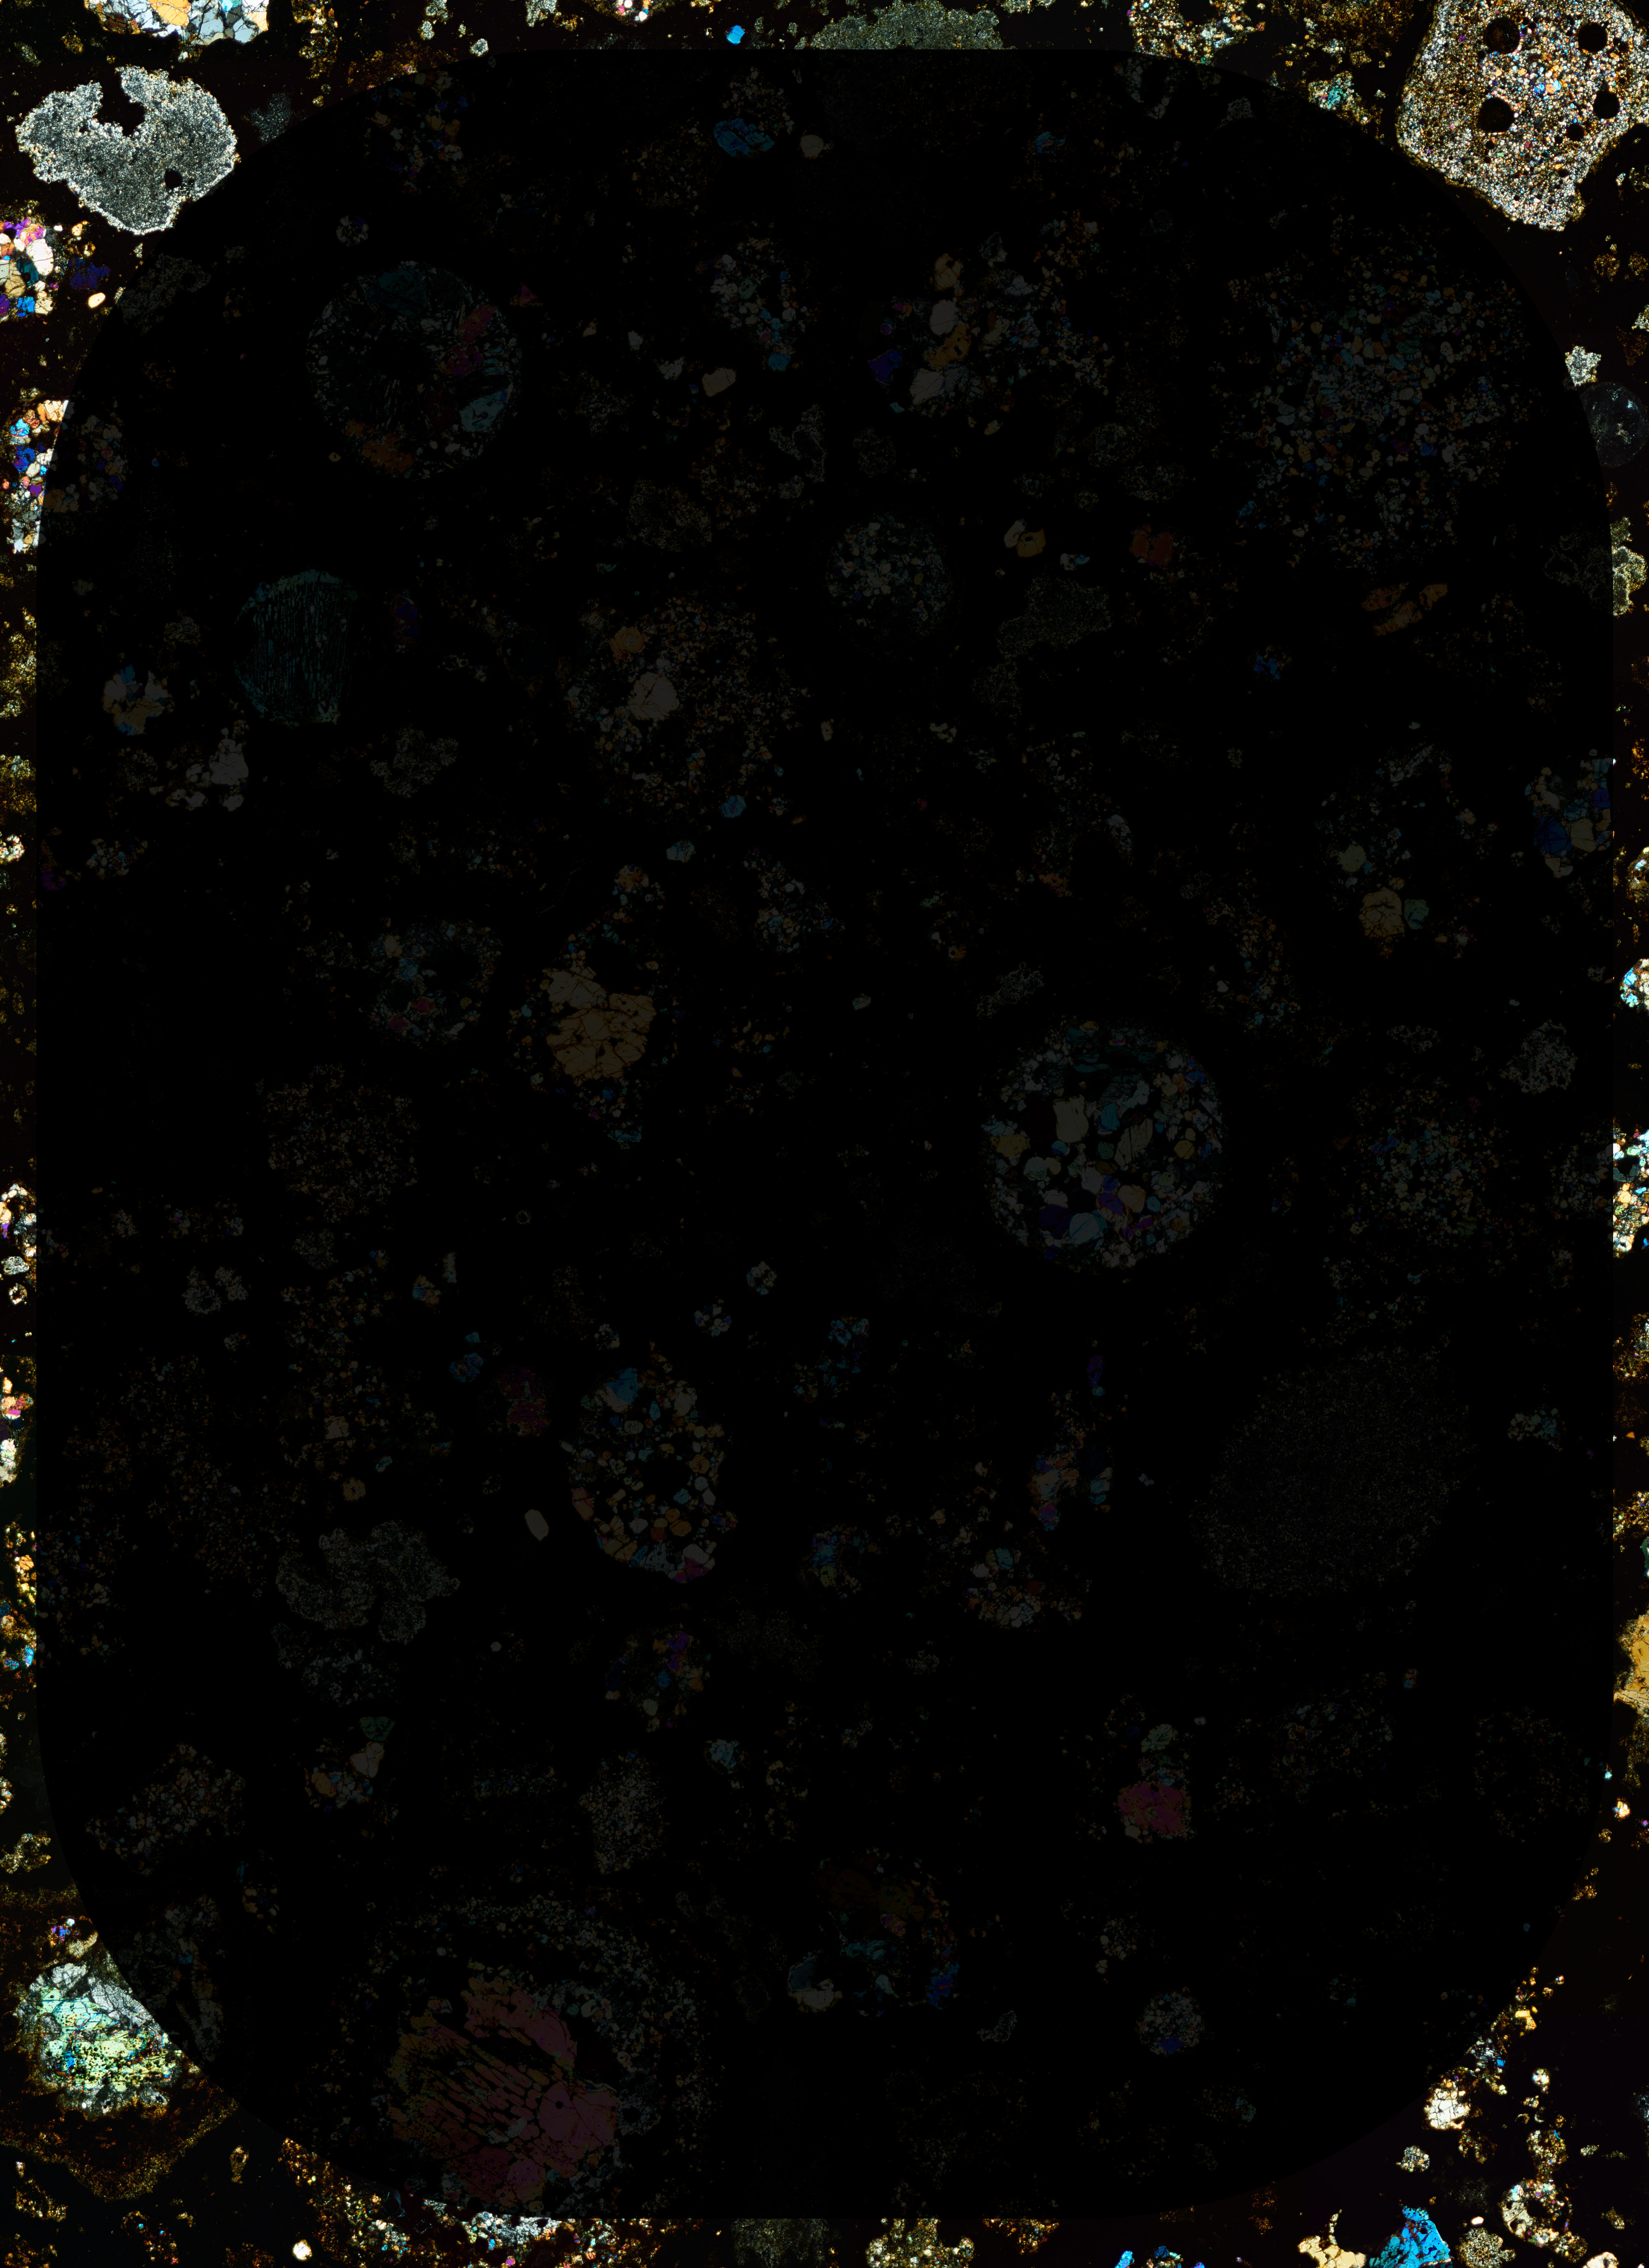
\includegraphics[width=\paperwidth,height=\paperheight]{Meteorite-Thin-Section-NWA2224-final-page-2.jpeg}}
\def\arraystretch{1.15}
\renewcommand{\thefigure}{{\arabic{figure}}}

\renewcommand\thefootnote{{\color{White}{\arabic{footnote}}}}
\let\oldfootnote\footnote
    \renewcommand{\footnote}[1]{\oldfootnote{{\color{White}#1}}}
\begin{titlepage} % Suppresses headers and footers on the title page
	\centering % Centre everything on the title page
	\tcshape % Use small caps for all text on the title page

	%------------------------------------------------
	%	Title
	%------------------------------------------------
	
	\rule{\textwidth}{1.6pt}\vspace*{-\baselineskip}\vspace*{2pt} % Thick horizontal rule
	\rule{\textwidth}{0.4pt} % Thin horizontal rule
	
	\vspace{0.75\baselineskip} % Whitespace above the title
	
	{\LARGE The Historical Debate\\[0.5cm] on the Chondrites} % Title
	
	\vspace{0.75\baselineskip} % Whitespace below the title
	
	\rule{\textwidth}{0.4pt}\vspace*{-\baselineskip}\vspace{3.2pt} % Thin horizontal rule
	\rule{\textwidth}{1.6pt} % Thick horizontal rule
	
	\vspace{1\baselineskip} % Whitespace after the title block
	
	%------------------------------------------------
	%	Subtitle
	%------------------------------------------------
	
	{Solar Anamnesis, Editor\\} % Subtitle or further description
	
	\vspace*{1\baselineskip} % Whitespace under the subtitle
	

	%------------------------------------------------
	%	Publisher
	%------------------------------------------------
		
	\vspace*{\fill}% Whitespace under the publisher logo
	
	\vspace{1\baselineskip} % Whitespace under the publisher logo

    Internet Archive Online Edition  % Publication year
	
	{\small Attribution NonCommercial ShareAlike 4.0 International } % Publisher
\end{titlepage}
\setlength{\parskip}{1mm plus1mm minus1mm}
\setcounter{tocdepth}{3}
\setcounter{secnumdepth}{4}
\tableofcontents
\clearpage
\listoffigures
\clearpage
\section{Foreword}
\subsection{``Fossil Organisms in Meteorites,'' by George W. Rachel}
\paragraph*{}
Dr. Hahn's work, of which \emph{Science} gave a short notice in its last issue, promises to revolutionize many views which have heretofore been believed to be firmly and irrevocably established. It is not at all necessary to accept all the conclusions and agree with all the various lines of reasoning, into which the author has been led by his results, but nobody will fail to perceive the portentous meaning of the results with which his untiring efforts in this important matter have been rewarded.

There has been formerly a manifest tendency to belittle small things and apparently insignificant phenomena, and bestow the greatest attention on those matters which impress the observer by their magnitude. Modern science has done away considerably with this erroneous method and has taught us that it is the little things which achieve great results in nature, as a rule. To this class of phenomena, which has been habitually underrated until a comparatively recent time, belong the meteorites, shooting stars and meteoric dust generally. [Ernst] Chladni's view that they fall from the skies, pronounced in 1795, was ridiculed by the learned men of the times. One member of a committee sent by the French Academy to investigate the fall of a meteorite in the neighborhood of L'Aigle\index{meteorite!L'Aigle}, [Jean-André] de Luc, declared that he would really be forced to believe what the people who witnessed the fall said, if he did not know that such a thing was \emph{utterly impossible}.

It was not long, however, until the celestial origin of these bodies was universally recognized, several other falls of large meteorites occurring during the first decade of the present century, which could no longer be explained away. After this various stones that were known to have fallen upon the Earth\index{Earth} were examined and described, and a good many more which were recognized to be of celestial origin. The number of all the various specimens thus investigated has gradually become very large. [Paul August] Kesselmeyer, in his great work on the subject, describes 647 distinct falls.

It is not now necessary to recall the several results of these investigations, nor to describe the peculiar properties of meteorites on which the resemblances and differences between those celestial minerals and our terrestrial rocks are based. Suffice it to state that between the two types which have been recognized, \emph{viz.}: those consisting exclusively of iron, and those which are composed of certain siliceous minerals, such as augite\index{augite}, bronzite\index{bronzite}, olivine\index{olivine}, anorthite and other feldspars, there are all the possible combinations of both; the ferrous meteorites predominate, however, those with a considerable percentage of siliceous constituents being comparatively rare, and the purely siliceous still more so.

It is the latter, the siliceous material, which has been examined with such remarkable results by Dr. Hahn. This occurs usually in light-colored spherical or pear-shaped masses (χονδροι [chondroi]) similar to the nests of crystals (druses) which are a well-known occurrence in crystalline rocks. These peculiar forms consist principally of bronzite and enstatite\index{enstatite}, which to the naked eye show an appearance graphically described by Kesselmeyer twenty years ago.

Professor [Carl Wilhelm von] Gümbel\index{Gümbel}, of Munich, in a report made to the Royal Bavarian Academy of Sciences has described them, on the basis of Kesselmeyer's book and his own researches, as follows:

``Longitudinal sections show columns and fibres, composed of small polyhedra, which in cross sections look like irregular polygons. These polygons often show a sort of radiating arrangement in their interior, issuing from what appears to be an ill-defined nucleus; this nucleus seems to have been changing its place gradually, for the radii show an irregularity such as would be produced by such change of site. The fibres, for that is what these structures look like, are not of equal size throughout, but taper off into points and occasionally even send off branches. This is especially visible in cross-sections where one set is apparently replaced by others, these in turn by others, and so on. All the fibres consist, as has been stated, of a light centre, and a dark enclosing substance.''

This description was given in 1878, and it certainly reads like what Hahn has proved it to be: \emph{fossil organisms!}\index{fossil}

This successful amateur, for such he was before he succeeded in gaining his present reputation by his participation in the debate on the ``\emph{Eozoön canadense}\index{Eozoön},'' and then resigned his government position to pursue this peculiar line of research at his leisure --- this ``Gerichts-Referendarius, a D.'' has by an ingenious application of the comparatively new method of making transparent sections of these meteorites accomplished results of which many a specialist might be proud. In order to exclude the error to which human vision and draughtsmanship might be liable, he has prepared photographic reproductions of his specimens, and on 32 excellent plates he presents the scientific world with 142 of these highly interesting preparations. Most of the fossil structures thus revealed belong to the animal world, indeed, Hahn himself professes that he is unable to find evidences of vegetable organisms; these, however, since the appearance of his work in February, have been recognized by Professor [Hermann] Karsten\index{Karsten}, of Schaffhausen, Switzerland, in sections prepared by him from a portion of the very meteorite in his possession which has furnished a considerable number of Hahn's specimens. Two of these Professor Karsten has drawn, and the cuts are published in an exhaustive paper on Hahn's book, together with his own observations and those of others on this very subject in the German Journal \emph{Die Natur}, edited by Mr. Carl Mueller, of Halle, Prussia.

As to the genuineness of Dr. Hahn's discovery there can be no possible doubt, and it has been generally admitted --- reluctantly by some, it is true --- that these ``chondrites'' consist almost exclusively of fossil\index{fossil} organisms. Dr. David F. Weinland, a member of the Academy of Sciences, of Philadelphia, where he formerly resided, has also published a review of Hahn's book in \emph{Das Ausland}, edited by Friedrich von Hellwald, of Tübingen\index{Tübingen}, Wurtemberg, in which he states that by the kindness of the author he has had the opportunity of examining these specimens, and although this examination has not given exactly the same results in regard to the determination of the particular kind of organism, he cheerfully admits that they are organisms, and this fact will not be doubted by any one who scans the plates published by Dr. Hahn.

In a postscript to this review, Dr. Weinland informs the reader that the author has entrusted to him the difficult task of classifying all the fossil organisms in more than three hundred of his specimens --- of which Hahn has prepared over six hundred --- and Dr. Weinland who is a competent naturalist, gives a few of his preliminary results. He compares the material which these sections display to the detritus of which the youngest coral\index{coral} lime and sandstone (coralline crag) consist such as is found on the shores of the Mexican Gulf. He furthermore states that complete forms are rarely found, but that the material is sufficiently abundant to construct many complete species, in the manner usually applied to fossil remains. 

The number of the various species of polypi, crinoids, sponges; and algae which are united by a siliceous material, Dr. Weinland estimates after a cursory examination at about fifty.

One of the corals is set down by various observers a resembling to the \emph{Favosites goldfussi} from the Silurian\index{Silurian} \emph{Grauwacke},\footnote{A drawing of this fossil\index{fossil} coral\index{coral} is given by Dana in his \emph{Textbook on Geology}, Ed. 1868, p. 111.} another is compared to the \emph{Calamopora naumanni} from the same strata.

The structure of these corals is excellently preserved; the columnar structure, the stomata, the rays in the cells, indicating the partitions between the columns in cross-sections, in short, all the various parts can be perfectly well demonstrated.

Of sponges Dr. Weinland has already determined three different genera. Of a peculiar bluish-colored sponge\index{sponge} he says he could draw a perfect picture, so numerous are the various longitudinal and cross-sections in which it occurs, it would be as easy as it would be to draw it from a living sponge\index{sponge}.

Algae have also been recognized as forming part of this intricate network of fossils. Dr. Weinland has determined several as belonging to the \emph{Cocconeis}, while Professor Karsten\index{Karsten} describes others belonging to the genera, \emph{Leptothrix}, \emph{Leptomitus} and \emph{Hysterophyma}. (The latter gentleman reminds the reader of the fact, that [Paul F.] Reinsch has lately demonstrated the existence of these and other algae in coal, some of his specimens containing as much as twenty per cent of such organisms.)

But what is the most interesting feature of all the organisms thus ingeniously and unexpectedly brought to light in meteorites is their Lilliputian size. The coral\index{coral}-tree, above referred to as a \emph{Favosites}\index{Favosites}, presents itself to the naked eye as a white spot on the section, not larger than a pin's head. Its greatest diameter measures nine-tenths of a millimeter, and the single cells not more than about five one-hundredths of a millimeter. All the other organisms detected show the same pygmean proportions, the spicules of sponges, for instance, being absolutely indefinable to the naked eye.

The origin and formation of these celestial fossils could not possibly have been different from what we know it to be with our terrestrial specimens. They tell us of a planet, on which aquatic life was sufficiently developed to produce them and to preserve them after death by a process of infiltration with siliceous material, which dissolved the lime of which these structures must have consisted as far as their inorganic constituents are concerned, and supplanted it by the various kinds of siliceous minerals, filling up also the interstices and openings which had formerly contained organic substance. This planet, therefore, must have had a comparatively long period of existence; it must have had an atmosphere and its surface must in whole, or in part, have been covered by water. What the cause has been of its destruction and its utter disintegration we are, certainly, unable to tell; but the meteoric stones which formed part of it have happily crossed the orbit of our planet and thus enabled us to divine its history, at least in part.

In connection with this subject, it may not be amiss to give a short synopsis of the history of our knowledge of organic constituents in meteoric stones.

The first to detect the existence of organic substance in meteorites was the great [Friedrich] Woehler. In the meteorite which fell on April 17\textsuperscript{th}, 1857, near Kaba\index{meteorite!Kaba} in Hungary, he found unmistakable traces --- while analyzing it --- of a combination of carbon and hydrogen. Then the fact was remembered that on Oct. 13\textsuperscript{th}, 1835, a fire ball had exploded in the neighborhood of Bokkeveld\index{meteorite!Cold Bokkeveld}, Cape Colony, scattering a great number of soft, black stones over the fields, weighing, as far as could be judged, several hundred pounds. These stones emitted a strong ammoniacal smell and were found to be impregnated with water and bitumen. Woehler obtained one of these meteoric stones and found that it contained, besides one and two-thirds per cent of carbon, a quarter of one per cent of organic matter proper.

Referring to this discovery, Friedrich Mohr wrote,\footnote{\emph{Geschichte der Erde}, 1866, p. 500.} sixteen years ago:

``This is sufficient proof that there was present in this meteorite a carbohydrate similar to our ozocerite, idrialite, seberrerite, mineral wax, \emph{etc}. According to our terrestrial experience we must therefore conclude that on the planet of which they formed part, there must have existed organisms, at least plants, which are the real cause of the many deoxidized combinations which we find in meteorites. The existence of plants would evidently condition the presence of free oxygen, which does not speak against the presence of these products of deoxidation, since the plants themselves require oxygen for completing their cycle, in so far as they are ultimately (by decomposition), retransformed into carbonic acid, without which condition a long, unbroken chain of vegetable life would be inconceivable. But the water must be liquid in order to act, and this implies that this planet must have had a certain size to enable it to be sufficiently warmed by the sun. The small meteorites, as they come to us, must in spite of their being exposed to the sun's rays, have the temperature of cosmic space, since they are, just as are high mountain peaks, too insignificant to become heated by insolation alone. Only an enlargement of size enables a celestial body to develop heat enough to produce a warm atmosphere. This circumstance supports strongly the view, that meteorites have not been formed independently, but that they have formed part of a larger body, on which processes, similar to those obtained on our planet, have been going on.''

This is certainly interesting reading today, knowing as we do that the planet in question has also been an abode of animal life.

Other meteorites containing organic substances have been recorded since then. Thus at Orgueil\index{meteorite!Orgueil}, France, 1864; at Knyahinya\index{meteorite!Knyahinya}, Hungary, June 9, 1866. This phenomenon is the most important since very many of the most convincing specimens, prepared by Dr. Hahn, have been obtained from a stone weighing 27 lbs., which formed part of the 600 lbs. that fell in that particular locality on that day.

The most curious meteoric shower, however, was observed in 1870 in Sweden. Black pieces, consisting almost exclusively of mold, descended on a snow-field, and could thus be easily collected. Mold is always the result of some organic process, and living particles play the efficient part in its production.

Since bacteria are known to be able to withstand a temperature of -100° C, without losing vitality, the Thompson-Richter hypothesis of the propagation of life through the universe in this manner becomes almost a tangible reality. But, we forbear! The perspective opened by Dr. Hahn's discovery is too grand to be discussed in the brief space, allowed this notice. It is only to be regretted that the favored discoverer seems inclined to tamper with his good fortune in so far as he draws conclusions from his newly established facts which few will be willing to admit. He thinks it possible that the formation of living matter may have begun in cosmic space, that cells were developed from chaos and a certain vegetative process could have gone on in the gaseous and liquid masses supposed to have been the formative matter of our solar system, \emph{etc}. Professor Karsten\index{Karsten} is even of the opinion that meteorites might form in the upper strata of our atmosphere. As proof he adduces the few recorded showers of polygonal hail-stones and especially the two cases of ice-meteorites. On May 28\textsuperscript{th}, 1802, there fell near Puztemischel, Hungary, a block of ice weighing 1200 lbs. and [Benjamin] Heyne in his \emph{Tracts Historical and Statistical on India} reports the fact that near Seringapatam a mass of ice fell from heaven, as large as an elephant, which took, in spite of the tremendous heat, over two days to melt.

If we should be asked our opinion as to what the origin of these ice-meteorites may have been, we should be inclined to answer that they are very probably a small part of the collections of water (oceans?) which, we know, must have existed on the disintegrated planet to which our stone and iron meteorites once belonged.

The various theories which have been held to explain certain well-known facts about meteoric bodies, notably [Giovanni] Schiaparelli's ingenious hypothesis connecting comets with meteorites, the fact that most comets give a spectrum, closely resembling that of carbon, and many others will have to be revised in the light of this discovery, and it may be safely claimed that Dr. Hahn's book will prove to be one of the most important contributions to natural science of the present time.
\clearpage
\subsection{``Mr. Darwin on Dr. Hahn's Discovery of Fossil Organisms in Meteorites,'' by G. W. Rachel}
\paragraph*{}
Dr. Hahn's discovery, of which an elaborate account was given in No. 50 of \emph{Science}, has stirred up a lively discussion of this highly interesting subject. Dr. Hahn has taken steps to enable Professor [Friedrich August] von Quenstedt\index{Quenstedt}, the renowned Tübingen\index{Tübingen} geologist, and all others who expressed the desire to examine his microscopic preparations. It is understood that all those who have availed themselves of the opportunity thus offered have become convinced of the genuineness of Dr. Hahn's discovery.

It is very interesting to note the position taken by the greatest of living evolutionists in this controversy, if it can still be called such. Charles Darwin, on receipt of Dr. Hahn's work, wrote to him:

``... It seems to be very difficult to doubt that your photographs exhibit organic structure ...,'' and furthermore:

``... your discovery is certainly one of the most important.''

Not content with the mere presentation of his work, Dr. Hahn visited the veteran zoologist and brought his preparations to him for inspection.

No sooner had Mr. Darwin peered through the microscope on one of the finest specimens when he started up from his seat and exclaimed:

``Almighty God! What a wonderful discovery! Wonderful!''

And after a pause of silent reflection he added: ``Now reaches life down!''

The latter remark no doubt refers to the proof furnished by Dr. Hahn's discovery that organisms can reach our planet from celestial space. It is an acknowledgment of the relief Mr. Darwin must have felt in not being forced to a belief in a primeval ``\emph{generatio equivoca}.''

As was suggested in the paper referred to, ``the Richter-Thomson hypothesis of the origin of life on the Earth has become a tangible reality!''
\clearpage
\section{\emph{The Meteorite (Chondrite) and its Organisms}, by Otto Hahn}
\subsection{Introduction}
\paragraph*{}
It was not the inconsequential attacks on my \emph{Primordial Cell}\index{Primordial Cell} that gave me stamina to establish certain new geological facts, but rather it was the untenability of all previous views regarding that undisputedly most important part of the geological sciences, the part through which it relates to the cosmos --- that is, in the doctrine of the so-called plutonic rocks.

If, in the first part of \emph{Primordial Cell}\index{Primordial Cell} I had tolerated the doctrine and with resignation accepted that the core of our Earth\index{Earth}, and with it the knowledge pertaining to its real genesis, will always remain hidden from us, then, at the end of this book there is yet a possibility: the meteorite\index{meteorite} indicates a passage from far away, although not yet actively pursued by researchers.

With this as a guide, I would like to continue.

I did it, accompanied on the one hand by sharply pronounced ridicule from the specialists, and on the other with joy from my earlier results and the now daily support and counsel from the few friends whom I have succeeded in convincing.

The results yielded from this strenuous endeavor of almost super-human effort over the previous year are laid down in the following pages.

It is a world of animals in a rock that arrived on Earth\index{Earth} to bring us tidings from the smallest beings of a most distant place --- a life-world which a mortal eye could hardly hope to behold: a world of beings showing us the creative power that made our Earth\index{Earth} out of a nebula and has worked universally and evenly in the universe.

Admittedly, the meteorites, namely the chondrites\index{chondrite}, for these are the ones which are preferentially subject to my investigations, contain no life of higher construction; rather, all are lower life forms --- the same ones which prevail in the Silurian\index{Silurian} strata --- sponges, corals, and crinoids --- it is with these species that similar characteristics are found.

The chondrites that I have studied are olivine\index{olivine} enstatite\index{enstatite} rock. They have undergone alterations, although not considerable, since the time of their formation as the remains of life up until landing on Earth\index{Earth}. They have been permeated with a silicate solution, in a similar manner to how the Jura\index{Jura} deposits are with a solution of lime. While it was part of the parent body it probably underwent planetary cycles, just as new layers follow old ones down to the lowest strata on Earth\index{Earth}, under the influence of which the former have undergone a certain, though not as considerable as one assumes, transformation.

Only the surface of the meteorites\index{meteorite} has changed considerably, indeed, only at the last moment of their planetesimal existence and mostly due to the influence of frictional heating created, in this case, by the Earth's atmosphere\index{Earth!atmosphere}. But the original meteorite\index{meteorite} itself essentially remains. We now see that before us is a piece of a planet as it was in the process of becoming, and thus the history of our Earth's\index{Earth} body is now open to us, provided that we are correct that the meteorites\index{meteorite}, in their formation, are homogeneous in their chemical composition with the world matter that formed the Earth\index{Earth} and vice versa. At the same time, by sending me the ``Meteorite of Ovifak\index{Ovifak}''\index{meteorite} (I owe it to the kindness of Professor Dr. von Nordenskjöld) I was offered the opportunity of bringing this rock into the investigation.

I consider it to be terrestrial --- as part of the deepest layer of Earth\index{Earth}, \emph{i.e.} the olivine\index{olivine} layer, which belongs under the granite. I call this original layer the Olivine\index{olivine} Formation. Since the rock is very similar to a meteorite\index{meteorite}, it is natural to declare it to be the same. The reasons why I do not consider it to be meteoritic but true to the Earth's core\index{Earth!core} are laid down in this book.

Thus, we have gained two solid points by which a lever can be set.

The chondrites\index{chondrite}, an olivine\index{olivine} feldspar (enstatite)\index{enstatite} rock, consist of an animal world; they are not part of a sedimentary rock layer nor a conglomerate, but a felt of animals, a fabric whose meshes were all once living beings and life of the lowest kind, the beginnings of creation.

However, I could not make a systematic enumeration of the life which is preserved in the meteorites\index{meteorite}: I just wanted to prove that it is so --- that is all. I therefore only depicted the organic beings that I was able to assure myself as determining undoubtedly: on the one hand the genera which coincide with terrestrial forms and, on the other, separating out the specifically meteoritic forms, while leaving both to future investigation.

It is to be expected that my enumeration will be, through further research and with the help of richer material than I have available, multiplied and supplemented. Subdivisions had to be avoided: since every newly discovered being would overturn any divisions and make the effort arduous with any work in vain.

This is the reason why I only made large divisions, and these only to the extent that this contributed to the understanding of the forms. I repeat, the work in this direction should not be considered exhaustive and complete.

In other ways I have also made an indulgence, such as in the demarcation of the main divisions themselves.

Anyone who even superficially surveys the forms will soon find that they provide an actual historical development. All the transitions from the sponge\index{sponge} to the coral\index{coral}, from the coral to the crinoid\index{crinoid} are present, so that it becomes doubtful if one should assign new species to these transitions.

In such beginnings mistakes are inevitable, so it is only a small demand in asking to forgive them. Nor did I want to delay the publication of this work too long and therefore have it just as it is now.
\clearpage
\subsection{History and Overview}
Δός μοι χέντρον%Δός μοι χέντρον
\paragraph*{}
Last year, when I wrote-down in my diary certain new observations about the composition of the rocks of our Earth\index{Earth}, and also of the meteorites\index{meteorite}, the importance of the latter to geology was not fully clear to me.

It was only when I was forced by the attacks of opponents to take the investigation again into my own hands that I clearly realized the importance that a careful study of the meteorites\index{meteorite} could be to the history of our Earth\index{Earth}. Lastly, I came to the conclusion that in the present state of geology the meteorites\index{meteorite} --- and only the meteorites\index{meteorite} --- give the point from which the history of Earth\index{Earth} could at last be explored with near certainty.

If in \emph{Primordial Cell}\index{Primordial Cell} I thought that I had reached the limit of research with granite, I soon learned better. I contemplated that by virtue of its specific gravity, the Earth's core\index{Earth!core} must also consist of at least solid iron, especially considering the very probable order of the meteorites\index{meteorite}, which go from the pure iron to the feldspar rocks of Earth\index{Earth}. I further believed that a conclusion for Earth\index{Earth} based upon the meteorites\index{meteorite} could be ventured, the conclusion that in the other planets and in those, or the one, whose \emph{débris} we have in the hundreds of thousands of orbiting meteorites before us we have a sequence of stratification from heavy to light, a stratigraphy which we probably pass through in the series from the pure-irons through the half-irons (Pallasite\index{meteorite!Pallasite}, Hainwood\index{meteorite!Hainwood}) to the chondrites\index{chondrite} and the eucrites\index{eucrite}, then to the coal meteorites\index{meteorite!coal} (Cold Bokkeveld)\index{meteorite!Cold Bokkeveld}.

Once this likelihood had been understood, it was obvious that the meteorites\index{meteorite} should be subjected to a thorough examination of their morphological characteristics. This was also highly necessary because so far almost nothing has happened in this direction: one can convince oneself of this by comparing my photomicrographs with the roughly twenty meager illustrations, which taken together form the material of the science today. The academic writings of Berlin\index{Berlin}, Vienna\index{Vienna}, and Munich have only a few panels each, the drawings are small, and it immediately shows, are taken from the least suitable meteorites\index{meteorite} for this direction of investigation and, moreover, probably not from the best part, the interior.

So if, I thought, my earlier assertion that the Knyahinya Meteorite\index{meteorite!Knyahinya} consisted entirely of life was not confirmed by my new investigations, then science would still have been served if I were to show the true nature of this meteorite\index{meteorite}. Fortunately, however, I was spared this retreat: on the contrary, the results of my new research were far beyond expectations --- a new world emerged.

But, of course --- science is skeptical --- it rightly demands more stringent evidence than I offered in \emph{Primordial Cell}\index{Primordial Cell}; a book written more at the stage of, I would say, intuition. Today I present the evidence.

As one examines the tables of this work, it immediately becomes clear that these are not mineral forms, but organic ones; that we have before us the images of life, images of life of the lowest order, a creation which in greater part finds some of its closest relatives here on Earth\index{Earth} --- regarding the corals\index{coral} and crinoids\index{crinoid}, this is determined with absolute certainty; however, the sponges\index{sponge} have only some similarity with those forms of the terrestrial genera.

Thus, the genesis is determined in terms of the parts. However, in my study of twenty chondrites\index{chondrite} (and 360 thin sections of them) the assertion made in \emph{Primordial Cell}\index{Primordial Cell} was confirmed --- that the rock of the chondrites\index{chondrite} is not a type of sedimentary rock as on Earth\index{Earth}, in which fossils\index{fossil} are embedded, that it is not a conglomerate formation; but rather, its whole mass is entirely formed of organic beings, like our coral\index{coral} rocks. So not a plant, as I had assumed earlier, but plant-animals! The whole stone is life: --- I think science will forgive me the first mistake.

Needless to say, the iron meteorites\index{meteorite!iron} were now subject to additional testing. Here it rests as only a first observation.

However, time and circumstances, especially the lack of available materials, prevented me from concluding the investigation prior to this publication. But if I repeat today the first assertion, that meteoritic iron is nothing but a mat of plants, then I may now regard myself as more legitimate than at the time when I wrote \emph{Primordial Cell}\index{Primordial Cell} and asserted the prior statement. I have to add that I also found life-forms in the irons. The researchers who avoid the forms of the chondrites that I depict may overlook the fact that the so-called Widmanstätten's\index{Widmanstätten} figures are, for the most part, plant cells and not crystals.

The investigations up till now, in the whole field, with the exception of [Carl Wilhelm von] Gümbel's\index{Gümbel} work in the Munich Academy, are of little use, both regarding the accuracy of their observations and even more their interpretations based upon those observations, \emph{i.e.} on unproven hypotheses and weak assumptions --- not suitable for scientific findings as such. And due to this the field was still wide open to me, although my only regret is that I cannot make a draft in time regarding the irons.

I now come to the conclusions for geology. If the chondrites, an olivine and enstatite\index{enstatite} rock, are really what I assert: that is, only pieces of sponge\index{sponge}-coral-crinoid rock, then a fact of immeasurable consequence has been discovered for the science of Earth\index{Earth}.

The feldspar minerals are a purely water production --- they are the petrifying matter of millions of organisms! Thus, all hypotheses about the metamorphic and plutonic rocks of Earth\index{Earth} fall, and with them the theory of the fire-liquid Earth\index{Earth} interior --- or at least no conclusion can be drawn from the rocks any more.

I now have to justify this. A comparison of terrestrial rocks with the meteorites shows that the chondrites, at least according to their chemical nature, have their closest relatives on Earth\index{Earth}.

The olivine\index{olivine} rock of Earth\index{Earth} is, as a lherzolite, a bedrock layer such as we see with basalt breaking through granite; I arrive at the results that [Gabriel Auguste] Daubrée has shown.

The deeper granite is definitely younger than the olivine\index{olivine}. But if the olivine\index{olivine} of the meteorites\index{meteorite}, by virtue of its composition, is a water-rock, it will probably be likewise for the granite of Earth\index{Earth}; if the olivine of the meteorites\index{meteorite} is the remains of life, then the same will be the case with the olivine\index{olivine} of the Earth\index{Earth}: it could probably be concluded then, that the rock of our Earth\index{Earth} is also composed in its original deposits of the same life as that of the chondrites. And for the same reason the granite, as younger rock, will probably have a similar origin. We only have to look at our Swabian basalts leaching through the original olivine\index{olivine} to see that the lherzolite bedrock is found under the granite. And even if this rock appeared as a liquid deposit without distinguishable forms, the iron of Ovifak\index{Ovifak} has such; but this is highly connected with the basalt, so intimately, and not only mechanically, that both must be regarded as one rock. So, this is the original olivine\index{olivine} bedrock. But because of this, scientific reasoning thus removes the presumption of the origin of the Earth\index{Earth} by way of fire.

If the surface of the planet, or of the planets, consists of layers of olivine\index{olivine} from life, then the same layers of our Earth\index{Earth} were probably not formed by fire, or at least there is not the slightest reason for this supposition; on the contrary, it should be assumed that the same layer of the Earth\index{Earth} was a water formation. Here I encounter the Kant-Laplace theory.

I imagine that the planetary materials (including water, which is usually overlooked) during the first mass formation were not, as [Immanuel] Kant and [Pierre-Simon] Laplace say, a glowing haze, but rather a vapor and mass as cold as space. Here, however, one has overlooked a great logical error in the above mentioned theory.

That the attraction of mass should form mass! That the effect should simultaneously be the cause! The mass is to be formed by mass attraction, that is, by the fact that it was already there! It is to be regretted that this error of thought has not been discovered earlier. A mass, when it is present, can increase through attraction, but not from it: it is as if someone should be his own father!

So another force had to have formed the mass; but this could only be either the crystallization force or the organic formative force.

The former does not suffice to explain the formation of the planets, and no crystals are found: consequently only the second force remains --- the organic one. Here I recall my observations on the structure of the meteorite\index{meteorite} and so today, for me at least, it is clear that the first beginnings of Earth\index{Earth}, and the rest of the planets, had an organic cause.

If the sentence appears a bit deafening, one need only resort to the familiar.

First, the mass of building materials available at the beginning of planetary formation is completely sufficient to explain the formation of the planetary mass in an organic way.

Secondly, the experience of today shows how, in short time, the lowest plants and animals multiply their number, including their mass, in a way that is conditioned only by the mass of the building materials, while their organization itself makes it possible to expand into infinity as long as building materials are present.

What seems to contradict this explanation is only the geothermal heat and the associated appearance of the volcanoes still active today. With regard to these two facts, one has long been led back to a different explanation, that of a liquid-fire Earth\index{Earth} interior. Water has a dissolving effect on feldspar. In this dissolving process, heat is released. The volcanoes follow the sea because water helps form the gases, which are ignited from above to melt the forthcoming rock.

How could a fiery Earth core\index{Earth!core} ultimately survive without oxygen! And does not the very existence of combustible gases (for these are the cause of volcanic phenomena), especially that of sulphur, indicate the presence of organic substances in the Earth's\index{Earth} interior? There really is no need for new evidence here, but only the abandonment of certain ideas, which have taken possession of the imagination excited by some obvious phenomena.

These are the conclusions from the study of the meteorites\index{meteorite} for our Earth's\index{Earth} formation. But the facts that astronomy can derive from them are no less significant.

The twenty meteorite\index{meteorite} (chondrite)\index{chondrite} thin sections that I have studied, some from falls which are more than a century apart, show the same forms, much as fossil\index{fossil} shells occur everywhere in the same formation; Gümbel\index{Gümbel}, if he did not correctly interpret the forms of the chondrites\index{chondrite}, has excellently expressed this.

So these chondrites\index{chondrite} are probably from one and the same world body, a planet. Or else how could evolution coincide on different planets?

This planet carries water life, so life has arisen in water and lives by water; this planet has not passed through fire, because the traces of fire do not show in these rocks. The meteorite\index{meteorite}, having been shattered, only receives a 1 mm. thick enamel fusion crust in its short path through our atmosphere as a result frictional heating.

The life of the chondrite\index{chondrite} is almost entirely a microscopic one, it ranges from 0.20 to a maximum of 3 mm. in diameter; often it takes a magnification of 1000x to clearly see the delicate structures, while at such magnification our terrestrial fossils\index{fossil} dissolve into a shapeless surface.

Thus, through the observations first laid down in \emph{Primordial Cell}\index{Primordial Cell}, the path was wide open for me to cover the distances that science must cross.

But it really doesn't take a titanium effort to destroy an old building. It has already been much worn, only ignored: it requires only one striking proof and the work will have been done. Traditions, based on insufficient observations, dissolve into what they are, allowing science to once again proceed freely on its course.
\clearpage
\subsection{Previous Views on the Meteorites\index{meteorite}}
\paragraph*{}
The following is a brief presentation on the previous views regarding the origin and nature of the meteorites\index{meteorite}.

Only the morphological work on individual meteorites\index{meteorite}, from the time when the microscope began to be used in geology, should be enumerated. What the microscope has so far provided for the interpretation of the meteorites\index{meteorite} is, apart from the enlarged olivine\index{olivine} crystals in [Nikolai Ivanovich] Koksharov's\index{Koksharov} \emph{Minerals of Russia}, Vol. 6, contained in the following writings:
\begin{enumerate}
    \item Gustav Tschermak\index{Tschermak} von Seysenegg: ``The Fragmentary Structure of the Orvinio\index{meteorite!Orvinio} and Chantonnay\index{meteorite!Chantonnay} Meteorites,'' presented at the meeting of The Royal Academy of Sciences (Vienna\index{Vienna}) on November 12, 1874. (20\textsuperscript{th} Volume of \emph{The Proceedings of the Royal Academy of Sciences}, Section 1, November Issue 1874, with 2 tables.)
    \item Alexander Makowsky\index{Makowsky} and Gustav Tschermak\index{Tschermak} von Seysenegg: ``Report on the Fall of a Meteorite near Tieschitz in Moravia.'' With 5 plates and 2 woodcuts, presented at the meeting of the Mathematics and Natural Science Class (The Royal Academy of Sciences in Vienna\index{Vienna}) on November 21, 1878. Volume 29 of memoranda of the mentioned class.
    \item Johann Gottfried Galle\index{Galle} and Arnold Constantin Peter Franz von Lasaulx\index{Lasaulx}, submitted by Christian Friedrich Martin Websky: ``Report on the Meteorite Fall at Gnadenfrei\index{meteorite!Gnadenfrei} on May 17, 1879.'' Session of July 31, 1879. Monthly Reports of The Royal Prussian Academy of Berlin\index{Berlin}.
\end{enumerate}
\paragraph*{}
The previous descriptions are limited to examinations with the naked eye and magnifying glass, as well as chemical analysis.

They all agree that the chondrites\index{chondrite!composition} consist of a matrix of spheres of enstatite\index{enstatite} (bronzite\index{bronzite}), olivine\index{olivine}, iron, nickel and chromite.

Gümbel\index{Gümbel}: ``On the Stone Meteorites Found in Bavaria,'' \emph{Proceedings of the Mathematical Physical Science Class of the Royal Academy of Sciences in Munich}, 1878, Issue 1, p. 14, \emph{et seq}. In the description of the meteorites of Eichstädt\index{meteorite!Eichstädt} and Schöneberg\index{meteorite!Schöneberg}, he mentions ``mesh-structure'' (p. 27 and 46). However, he also speaks of ``descendants of larger broken chondrules'' (p. 28). The important section of his observation is on page 58, which follows here:

``If one examines the results of the investigation of this, albeit limited, group of stone meteorites\index{meteorite}, then the perception that comes to the fore is that, in spite of some differences in the nature of their conglomeration, they are nevertheless governed by completely identical structural relations. All are undoubtedly \emph{débris}, composed of small and large mineral grains, from the well-known roundish chondrules: which are usually completely preserved, but often appear as broken pieces, to the globs of metallic meteoritic substances, sulfur-iron, and chromite. All these fragments are glued together, not cemented by an intermediate substance or a binder, as there are no amorphous, glassy, or lava admixtures at all. Only the fusion crust and black constrictions, which often appear on clefts and are similar to the crust, consist of amorphous glass, which, however, originated after falling within our atmosphere. In this melted crust, the denser meltable and larger mineral grains are usually still embedded unmelted. The mineral splinters do not bear any traces of rounding or tumbling, they are sharp-edged and pointed. As for the chondrules, their surface is not smooth, as it would have been if they were the product of tumbling, rather it is always uneven, mulberry-like and warty, or multifaceted with a projection of crystalline surfaces. Many of them are elongated with a distinct tapering or sharpening in one direction, as is the case with hailstones. Often you encounter pieces which apparently must be regarded as parts of shattered chondrules. As an exception are twin-like connected beads, most common in those which meteoritic iron beads have grown. In numerous thin sections they are composed differently. Most often there is an eccentric, radiating fibrous structure which spreads from a point far from the center after tapering or slightly tattered lines spread like rays toward the outside. Since cuts made at various angles always reveal a columnar or needle-shaped arrangement, never leaves or lamellas in the substance forming these tufts, it seems to be columnar fibers from which such chondrules are built. With certain cuts, according to this assumption, in the cross-sections of the fibers that are perpendicular to the length direction, only irregularly angular minute fields are observed, as if the whole was composed of small polyhedral granules. Sometimes they appear as if there were several systems radiating in different directions in a sphere, as if the point of radiation were altered during its formation, so that a constant and seemingly confused elongated structure emerges. Towards the outside, against which the junction point of the radiating bundle is shifted unilaterally, the fiber structure normally becomes indistinct or replaced by a more granular aggregate formation. In none of the numerous ground-up chondrules could I observe that the tufts ran directly to the edge, as if the point of emission were outside the sphere, provided that it was completely preserved and not a mere shattered piece. The delicate transversely dividing fibers usually do not run along the entire length of the tuft, but rather they gradually sharpen, branch or end to allow others to take their place, so that in the cross-sections, a manifold, mesh-like or netted image is created. These fibrils consist, as has often been described above, of a mostly lighter core with a darker envelope that is dissolved by acids, while the latter resists. Highly curious are the bowl-shaped constructions, which seem to be meteoritic iron, that are generally only spread over a small part of the globules. The same unilateral striations, visible on the average as crescent bowed streaks, also appear inside the chondrules and provide strong evidence contrary to their being formed by a tumbling of some material, the entire arrangement of the tufted structure speaks to a resolution against their origin by tumbling. However, not all chondrules are the eccentric fibrous type; many, especially the smaller ones, have a fine-grained composition, as if they are composed of a mass of aggregated dust. Here too, the one-sided formation of the spheres is sometimes noticeable by an intensely greater compression of the dust pieces.''

And further, p. 61:

``The most common type of stony meteorite\index{meteorite} is predominately that of the so-called chondrites\index{chondrite}, the composition and structure of which coincide so much that we do not see how a common origin and the initial cohesion of these chondrites\index{chondrite} --- if not all meteorites\index{meteorite} --- could be in doubt.''

``The fact is that they enter our atmosphere as highly irregular pieces --- apart from the shattering within into several fragments, which is common, but cannot be assumed in all cases, especially if, by direct observation the falling of only a single piece is confirmed; it can be further concluded that they make their orbits in the heavenly space as demolished pieces of a single larger celestial body and in their absent-mindedness occasionally fall to Earth\index{Earth} when they enter into the region of Earth's\index{Earth} attraction. The lack of original lava-like amorphous constituents in connection with the external irregular form is likely to exclude from the geo- or cosmological points of view the assumption that these meteorites\index{meteorite} are ejections of lunar volcanoes, as is often claimed.''

Gümbel\index{Gümbel}, having placed the meteorites\index{meteorite} as related to the olivine\index{olivine} rocks of Earth\index{Earth}, summarizes his view on their origin (p. 64) in the sentence: ``Therefore, the meteorites\index{meteorite} appear to be a kind of first process of encasing the celestial bodies, but since they contain metallic iron --- to have been produced in the absence of oxygen and water.''

``So ingenious,'' he continues (p. 68), ``...are these hypotheses of Daubrée's and Tschermak's\index{Tschermak} (origins from shattered volcanic rock), however, I cannot agree with their view on the formation of the globules (chondrules)\index{chondrite!chondrule} on the basis of my latest research. Contrary to Tschermak's assumption, I sought to prove that the internal structure of the chondrules is not out of context with their spherical shape and that these globules cannot be regarded as pieces of a mineral crystal or solid rock. Their unsmooth, unpolished surface stands out, which, if they were formed by abrasion or tumbling, should be mirror-smooth due to the similar hardness of the material, while instead it appears rough, bumpy, often facially striated, against the theory of friction, and there is no reason at all by which to understand why the other mineral fragments are rounded like grains of sand, and why, in particular, the meteorite\index{meteorite}, the iron, and the very hard chromite, as I have been convinced in the meteorite\index{meteorite} of L'Aigle\index{meteorite!L'Aigle}, are always not rounded, with often extremely finely sliced forms. How is it conceivable that, as if often observed, there would be a concentric accumulation of meteoritic iron within the globules? Also, the eccentric fibrous structures of most globules in their one-sided radiating do not appear to be random in relation to the surface, but rather like the nature of the structure of hailstones. This inner structure is closely related to the act of its formation, which can only be explained as a growth of mineral forming substances with simultaneous rotation in gaseous vapors that provided the material for further support, whereby more material began in the direction of movement.''

Gümbel\index{Gümbel} goes on to say that the material constituting the chondrites\index{chondrite} was formed by a disturbed crystallization and fragmentation resulting from explosive processes within a space filled with vapor and hydrogen gases supplying the minerals. He closes p. 72 with a discussion of the Kaba meteorite\index{meteorite!Kaba}:

``Perhaps, however, it is still possible to prove the presence of organic beings on extraterrestrial bodies.'' I hope this is successful. From his illustrations one can see that the investigation was based on bad material. After all, more thin sections should have been made and the magnification is far from enough. What I refer to is the upcoming description of my tables.

What I value so highly in Gümbel's\index{Gümbel} report is the scrupulous prejudice-free, let's say impartial, observations. I have allowed myself to quote the work of Gümbel\index{Gümbel} literally because it is indeed difficult for me to summarize such representations and to separate fact from interpretation.

Proper observations and incorrect explanations are so closely intertwined that it is impossible to do both. I thought while I read Gümbel's\index{Gümbel} paper (after completing my own investigations and manuscript) that I was coming to step on my conclusions at every moment. But, just as the surge of the surf seizes and throws back the man who wants to reach the shore, while with each attempt he thinks he has made it, so also here: the old dogma always pulls the honored researcher from the saving cliff into the sea and into the bottomless whirlpool of traditions.

Daubrée's commendable work \emph{Experimental Geology} was obtained only in translation and after completion of my work. No one will find that it refutes my conclusions. Daubrée himself depicted Knyahinya\index{meteorite!Knyahinya}: pressed, melted, dissolved, calculated, only not --- seen.
\clearpage
\subsection{Meteorites\index{meteorite} and their Mineralogical Properties}
\paragraph*{}
The literature on meteorites\index{meteorite} is very extensive. However, it is so well known in terms of the type and number of chemical compositions, that I do not need to dwell on this part of it, in particular the earlier works.

The meteorites\index{meteorite!classification} are divided into iron and stone, but there is still a class between the two: ``half-iron,'' \emph{i.e.} a combination of solid iron and stone --- the pallasites. While the irons show many similarities, both in their chemical composition and in the form of their structure, the pallasites are very different (depending on the predominance of iron). But there are other differences among them. Hainholz\index{meteorite!Hainholz} [mesosiderite]\index{meteorite!mesosiderite}, for example, has a blue mineral (enstatite)\index{enstatite} in addition to iron and olivine\index{olivine}, and in this a great richness of life-forms. The stones are divided into chondrites\index{chondrite}, stannerites [Stannern meteorite\index{meteorite!Stannern} --- eucrites], luotolaxers [Luotolax meteorite\index{meteorite!Luotolax} --- howardites], bokkefelders [Cold Bokkeveld meteorite\index{meteorite!Cold Bokkeveld} --- carbonaceous chondrites]\index{chondrite!carbonaceous}, bishopvilles [Bishopville meteorite\index{meteorite!Bishopville} --- aubrites], (Quenstedt, \emph{Klar and Wahr}, p. 280 following).

I prefer to study the chondrites\index{chondrite}, and where I speak of meteorites\index{meteorite}, I am referring to this class of stone meteorites\index{meteorite!stone}, which is also the most abundant.
\paragraph*{}
I have examined:
\begin{center}
\begin{tabular}{ l r }
 Tabor, Böhmen [Czech Republic] & July 3, 1753\index{meteorite!Tabor} \\
 Siena, Toskana [Italy] & June 16, 1794\index{meteorite!Siena} \\
 L'Aigle, Normandy [France] & April 26, 1803\index{meteorite!L'Aigle} \\
 Weston, Connecticut [USA] & December 14, 1807\index{meteorite!Weston} \\
 Tipperary, Ireland & November 23, 1810\index{meteorite!Tipperary} \\
 Blansko, Brünn [Czech Republic] & November 25, 1833\index{meteorite!Blansko} \\
 Château-Renard, Loiret [France] & July 12, 1841\index{meteorite!Château-Renard} \\
 Linn [Marion] County, Iowa [USA] & February 25, 1847\index{meteorite!Marion County}\index{meteorite!Linn} \\
 Cabarras [Monroe] County, North Carolina [USA] & October 31, 1849\index{meteorite!Monroe County}\index{meteorite!Cabarras} \\
 Mezö-Madaras [Romania] & September 4, 1852\index{meteorite!Mezö-Madaras} \\
 Borkut, Hungary & October 13, 1852\index{meteorite!Borkut} \\
 Bremervörde, Hanover [Germany] & May 13, 1855\index{meteorite!Bremervörde} \\
 Parnallee, East India [Tamil Nadu] & February 28, 1857\index{meteorite!Parnallee} \\
 Heredia, Costa Rica & April 1, 1857\index{meteorite!Heredia} \\
 New Concord, Ohio [USA] & May 1, 1860\index{meteorite!New Concord} \\
 Knyahinya, Hungary & June 9, 1866\index{meteorite!Knyahinya} \\
 Pultusk, Warsaw [Poland] & January 30, 1868\index{meteorite!Pultusk} \\
 Orvinio [Italy] & August 31, 1872\index{meteorite!Orvinio} \\
 Simbirsk [Russia] & [1838]\index{meteorite!Simbirsk} \\
\end{tabular}
\end{center}
\clearpage
\paragraph*{}
All rocks are thoroughly certified. Above all, I have the kindness of my revered teacher, Professor Dr. [Friedrich August] von Quenstedt\index{Quenstedt}, who thanked me with the excellent Tübingen\index{Tübingen} University Collection (which, as is well known, originates for the most part from [Carl Ludwig] Baron von Reichenbach\index{Reichenbach} in Vienna\index{Vienna}).

Of Knyahinya\index{meteorite!Knyahinya} I own 360 thin sections, of L'Aigle\index{meteorite!L'Aigle} 6, of Pultusk\index{meteorite!Pultusk} 6, of the remaining 1-3 each. I will name all stones after their place of fall. While making the thin sections, I made cuts in two directions. After several attempts on Knyahinya\index{meteorite!Knyahinya}, it turned out that it breaks in certain directions.

This was deduced from the inclusions that, once their positions had been found, regularly resulted in certain forms, to which these forms corresponded in sections made perpendicular to this position.

The forms of the stone were situated in such a way that the same position in the remaining stones would have been obtained, provided, of course, that the material had been available. For some, this happened by chance, while not in others; but for the reasons stated above further determination is required in this direction.

Also, I deliberately made the thin sections in three different thicknesses: thickly translucent, in order to see whole inclusions as completely as possible; very thin, in order to clarify the structural relationships; and for the majority, in such a way that both are still visible.

I would like to make a comment here, which will be confirmed by anyone who has dealt with thin sections of fossiliferous\index{fossil} material.

Only in rare cases of total transparency, \emph{i.e.} cut very thin, is the structure visible. Anyone who looks at a thin section, if cut in this manner, with the microscope will be delighted at the beautiful shapes and lines. At the joy of this, one will want to make things even better and one expects with continued grinding a perfect picture. But when one puts the thin section under the microscope after this second try --- there is nothing left but an almost structureless surface, with hardly hinted, even blurred shapes, and those which you previously perceived with the magnifying glass can no longer be seen, not even with the microscope. However, this phenomenon is related to the type of metamorphosis of the rock and the forms within it. The matter is well-known and therefore does not require further explanation. I only mentioned this matter so that those who want to make such observations will not be surprised and will improve their own manner of observation.

The fact that the chondrites\index{chondrite} consist for the most part of bronzite\index{bronzite}, enstatite\index{enstatite} (augite\index{augite}), and olivine\index{olivine}, as well as being magnetic throughout, is an accepted fact in the science. Quenstedt\index{Quenstedt}, \emph{Handbook of Mineralogy}, p. 722.

However, the inclusions that I claim are coral\index{coral} have been addressed as enstatite\index{enstatite}. This was believed to be able to explain their structures. Others went further and explained the inclusions as a type of glass (Tschermak)\index{Tschermak}.

So, before getting to the justification of my view, the microscopic appearance of the primary mineral, enstatite\index{enstatite}, must be clearly identified.

Allow me to give a brief outline of what [Carl Heinrich Ferdinand] Rosenbusch\index{Rosenbusch} says in his book: \emph{Microscopic Physiography of Petrographically Important Minerals}, Stuttgart 1873, p. 252, about enstatite\index{enstatite} (and bronzite):

``As is known, since the optical investigations of [Alfred] Des Cloizeaux\index{Des Cloizeaux}, enstatite\index{enstatite}, bronzite, and hypersthene\index{hypersthene} have been treated as rhombically crystallizing separated from pyroxene and compiled into their own group. In addition to the cleavage above the prism of 87°, the same shows further divisions above the vertical pinacoid, the relative perfection of which the data of various researchers do not exactly match. Chemically, these three minerals form an uninterrupted series, at the beginning of which stands the almost iron-free enstatite\index{enstatite}, and at the end of which stands the very iron-rich hypersthene\index{hypersthene}. Additionally, enstatite\index{enstatite} and bronzite are so similar in all physical properties that it is difficult to separate them into two species. Hypersthene, on the other hand, shows a different optical orientation and therefore forms its own species. It is interesting to note that Tschermak's\index{Tschermak} arrangement of the negative angles of the optical axes and the iron content of the three minerals mentioned makes it clear that the angle of the optical axes decreases steadily as the [iron oxide] FeO content increases. The microstructure of all the minerals of the enstatite\index{enstatite} group is generally so similar that, in special cases, a safe decision can only be made by chemical and precise optical analysis.''

``Enstatite\index{enstatite} and bronzite\index{bronzite} are not found in the rocks as crystals, but almost always in irregularly limited crystalline grains, which usually show a very dense striation, which is more straightforward in the case of enstatite\index{enstatite}, more gently winding and wave-like in the latter. But this difference is not a pervasive one. The same striation is also shown by the monoclinic diopside and rhombic bastite, which cannot easily be separated from bronzite by other, later to be discussed, visual phenomena. If the cut meets the enstatite\index{enstatite} or bronzite at a strong incline to the main cleavage surface, then the surface will not be equally fine-grained, but rather like a rough stairway. Transverse surfaces and fractures are not uncommon.''

``Both are relatively poor in extraneous deposits; they are missing, for example, in the enstatite\index{enstatite} from pseudophites of the Aloysthals in Mähren and in some enstatites\index{enstatite} or bronzites of the lherzolites and olivines\index{olivine}. The former is traversed only by frequent veins of pseudophite, from which fine-grained decomposition products penetrate the enstatite\index{enstatite} in a vertical direction. Other occurrences and even other individuals of the same hand specimen often contain mass inclusions of green or brown lamallae, splints, and grains (depending on the position of the grinding plane) which, without exception, are invariably parallel to the most perfect cleavage direction. This suggests the idea that various indications about the relative perfection of the pinacoid ($\infty$ P $\infty$) cleavage compared to the prismatic one may be due to the more or less mass presence of these interpositions, which undoubtedly also determine the metallic shimmer on the brachypinakoid. Then, however, the ease of separation in this direction would be more a separation than true fissility.''

``The enstatite\index{enstatite} without, and the bronzite with metallic shimmer on the brachypinacoid cleavage surface, can be found in the serpentines of Aloysthal in Mähren (enstatite)\index{enstatite} and Mont Bresouars in the Vosges, in the lherzolites and olivine\index{olivine} rocks, in some olivine\index{olivine} gabbros, in Streng's Enstatitfels from Radauthal near Harzburg\index{Harzburg} and in the olivinite bombs of the Dreiser Weiher [Daun area of Germany], as well as in some meteorites\index{meteorite}; so always in the company of olivines\index{olivine} and altered olivines\index{olivine}.''

For those who have command of the book, I provide two illustrations, one of bronzite\index{bronzite} from Kupferberg\index{Kupferberg} (Table 1: Figure 1), the other of enstatite\index{enstatite} from Texas\index{Texas} (Table 1: Figure 2), which are quite similar to Rosenbuschite.

As far as olivine\index{olivine} is concerned, there is no need for a picture, since the forms of this mineral are completely encompassed with circles. Suffice it to say that pure olivine\index{olivine} does not show any structure. Olivine\index{olivine} only shows structure if one wants to call its inclusions, or growth sites of the crystal, or decomposition phenomena (serpentine formation), structures. However, there is certainly no crystal that looks similar to my forms. As for the claim that the spheres are glass, it is not even made clear what chemical composition these glass spheres should have, compared with enstatite\index{enstatite}, bronzite, and olivine\index{olivine}. Apparently, all forms are thrown together and declared as glass, although enstatite\index{enstatite}, according to Quenstedt\index{Quenstedt} (\emph{Mineralogy}, p. 318), is infusible, and according to Naumann-Zirkel, p. 585, it is, at least, difficult to melt. It is even claimed that these glass spheres were first created while falling. But the effects of fire are found only in the fusion crust. The fusion crust of most meteorites\index{meteorite!fusion crust} is barely 2 mm. thick.

To the assertion that the chondrules\index{chondrite!chondrule} are glass, which is countered by the message sent by my thin sections, comes the reply that there are similarities of the meteoritic form with glass in the rocks of Earth\index{Earth}. Thus, I was referred by [Ferdinand] Zirkel to a spherulite\index{spherulite} liparite of which I give in Table 1: Figure 3. This form should show that my \emph{Urania}\index{Urania} is a deception. I think the form in the liparite is a crystallite\index{crystallite} formation (probably zeolite). Now look at the structures on Table 1: Figure 4, 5, 6!

Our researchers, apart from Gümbel\index{Gümbel}, speak of the meteorites\index{meteorite} as volcanic bombs, declaring the rock as identical to the volcanic rocks of Earth\index{Earth} and so counting the meteorite\index{meteorite} without hesitation with the volcanic rocks. The evidence to the contrary is the subject of this book.

Rightly, Quenstedt\index{Quenstedt} alone has declared the question an open one when he said: ``...it is reserved for the microscope to solve the riddle of the composition of the meteorites!\index{meteorite}'' \emph{Handbook of Mineralogy}, p. 722.
\clearpage
\subsection{The Organic Nature of the Chondrite\index{chondrite!organic}}
\subsubsection{Organic or Inorganic?}
\paragraph*{}
In order to prove that a plant or animal organism is present, I consider it necessary to prove:
\begin{enumerate}
    \item a closed form,
    \item a recurring form,
    \item recurring in developmental stages,
    \item structure, either cells or vessels,
    \item similarity to known forms.
\end{enumerate}
\paragraph*{}
If these requirements are valid, it remains only to decide whether plant or animal? Now ask yourself, do my forms fulfill these requirements?

I believe, before I go to the positive proof, that the negative proof ought to lead.

You see, the proof that I claim for the existence of organic beings is twofold: a negative one, by showing that the meteoritic forms do not belong to the mineral kingdom, and a positive one, by showing the similarity of the meteoritic forms with those of Earth\index{Earth}, whether living or extinct. The first thing to prove, therefore, is the following sentence:

The inclusions in the meteorites\index{meteorite} are not mineral formations.
\begin{enumerate}
    \item Our mineralogists explain the inclusions of chondrites\index{chondrite} as enstatite\index{enstatite}, bronzite, and olivine\index{olivine}. 
    
    Olivine\index{olivine} has no visible sheet breakage, but in enstatite\index{enstatite} and bronzite it is obvious. I depict a bronzite from Kupferberg\index{Kupferberg}, Table 1: Figure 1, an enstatite\index{enstatite} from Texas\index{Texas}, Table 1: Figure 2 (thin section at 75 times magnification). Figure 2 shows a good sheet fracture. Now compare this with Table 1: Figure 4, one of my favorites from the Knyahinya Meteorite\index{meteorite!Knyahinya} (about 250 times enlarged) and you will probably no longer speak about the fact that sheet breakage is the cause of the structural phenomena of the chondrites\index{chondrite}. Now look at all the tables and this explanation will be put aside once and for all.
    \item The inclusions of the chondrites\index{chondrite} consist of enstatite\index{enstatite} or olivine\index{olivine}; or they are glass: if this is the case, I ask, how is it possible that the same mineral, or glass, as a whole occur in such different forms (outlines and structures), and different minerals occur in such acutely coinciding forms? Look at hypersthene\index{hypersthene}, hornblende\index{hornblende}, augite\index{augite}! Apart from some visible, easy-to-explain inclusions --- (and this is not the case here) it is always the same picture! Here we have at most three minerals with a hundred different images!
    
    A mineral is simple, it must be simple in its expression and therefore always gives the picture of a homogeneous mass (field), with some inclusions at most. How could the same mineral be present in such different structures, in such coherent forms that differ from crystal forms?
    \item Minerals are either crystallized or not crystallized. In the first order they have a certain regular and recurrent form: they move along surfaces which, on average, project themselves as straight lines. These forms (lines and angles) are recurring, varying only in size, not ratio. Such forms are not found among the forms I have addressed as organic. In the organic forms there is no form with a surface or an angle; all are spheres or ellipses with deviations from a mathematical form, deviations that are nevertheless constant. It is these other forms which give rise to the need to foresee just what these matching structures are, showing themselves with constant outlines, these forms which are different from the crystal form of the enstatites\index{enstatite} and olivines\index{olivine}.
    
    Though they are rare, small sections are true crystals, but in a way, they are probative values that do not impinge on the facts. See below and Table 32: Figure 2.
    \item If the minerals were originally crystallized but happened to lose their crystalline form due to some mechanical force, the only form that could be repeated is the sphere or one approaching it, such as an ellipse. Here a repetition would be possible without a conclusion being drawn about the form. In these spheres, surface cuts of the body would immediately show the influence of such mechanical forces as the inclusions would be hit arbitrarily.
    
    However, the structure in the meteorite\index{meteorite} inclusions is always, I would like to say: symmetric, in harmony with its outlines.
    \item When crystals are weathered the layers change from the outside to the inside --- concentrically --- but there is no trace of weathering in the inclusions of the chondrites\index{chondrite} and their structures are always eccentric.
    \item Regarding the mineral inclusions, they provide different sights depending on their nature. The deposits have quite arbitrary forms, such as glass-liquid-inclusions and crystallites\index{crystallite}.
    
    But where crystal laws appear in the inclusions, they always depend on the crystalline form. This is not the case with meteoritic forms. No trace of inclusions in accordance with crystalline forms!
    \item A sheet breakage is only visible if a mechanical force creates a surface for light refraction phenomena. Without this, it is imperceptible. If cleavage surfaces are not present, light refraction phenomena do not reveal the meteorite\index{meteorite} inclusions, just ``dust material.''
    
    One finds in terrestrial minerals that there are interpositions parallel to the sheet cleavage: these do not show in the meteorites\index{meteorite}.
    
    I believe that the sight of my forms will make further discussion about the diversity of mineral and crystal images unnecessary.
    \item But so much has been said of crystallites\index{crystallite}, of crystallization.
    
    It has been previously held that such crystallization will turn into the enstatite-bronzite-olivine\index{olivine}\index{enstatite} spheres. Gümbel\index{Gümbel} pointed out that all spheres have eccentric centers!
    
    Here the idea about the basic difference between meteoritic forms and crystallites\index{crystallite} is made quite clear.
    
    Crystallites always grow around one point (concentric). The forms in the meteorites\index{meteorite} are all elliptical and pear-shaped: if the outer form is also spherical, the alleged inclusions are eccentrically arranged and the center lies on the periphery (even beyond it, namely, it is ground away, which Gümbel\index{Gümbel} overlooked) --- a phenomenon that never occurs in the mineral kingdom. It is precisely the condition of crystallites, \emph{i.e.} sphere formation, that crystals unite with a crystal of equal mass, which then create the concentric forms.
    
    Therefore, if the spheres in the meteorites\index{meteorite} were crystallites\index{crystallite}, then, at least according to the laws of Earth\index{Earth}, concentric formations should show.
    \item Finally, I must point out a contradiction that science came up with in order to explain the structure of the chondrites\index{chondrite} as being a mineral property. This is the optical behavior of these inclusions.
    
    If they are crystals and have broken sheets (of course olivine\index{olivine} has none, yet there are structures in the alleged olivine\index{olivine} sphere structures, \emph{i.e.} sheet fractures!) as the source of their structure, the mineral should by necessity refract light. In most of the inclusions, however, there is no refraction of light, not even aggregate-polarization\index{polarization}! So, they can neither be simple minerals nor crystals, nor, least of all, be sheet fracture structures. This matter, that of the optical behavior, should have already led to the correct interpretation.
\end{enumerate}
\paragraph*{}
All this evidence is of course unknown to the botanist and zoologist, while every mineralogist knows it. Therefore, I must ask the botanist and zoologist colleagues to confirm what my photographs show. These forms are not mineral forms. With this the mineralogist has done his part, and now it passes into the hands of the paleontologist, or rather the zoologist, and now begins the positive proof.
\clearpage
\subsection{The Individual Forms: Sponges --- \emph{Urania}\index{Urania}}
\paragraph*{}
Rounded, lobed bodies with an obvious place of growth. Table 2 gives a larger image of an \emph{Urania}\index{Urania} (compared with Table 5: Figure 1, the same picture). One sees here: the acute general form, the outermost lobed edge (white, on the left), the folds, which developed while contracting, the place of growth. Even more clearly is the latter as a chalice, Table 4: Figure 3.

Consolidated spiral-form \emph{Urania}\index{Urania} Table 3: Figure 5 and 6.

In comprehending the threads of Table 4: Figure 1 the structure consists of an outer membrane enclosing lamellar layers, Table 3: Figure 4. Table 4: Figure 6 (the latter can be seen with a magnifying glass). Median diameter of \emph{Urania}\index{Urania} 1 mm., color slate gray.

This structure was maintained to be a breakage of the bronzite\index{bronzite} sheet! Whether Table 4: Figure 4 belongs to the \emph{Urania}\index{Urania} is doubtful. The form and color suggest as much. The trim cuts on both sides show clear structure.

Table 5: Figure 5 shows entirely winding lobes. Either it is a hoisted spiral-form body, or it is several lobes, of which the outer one surrounds the inner.

Table 4: Figure 6 is a cross section, which does not show much. In the object itself you can see an average uncolored outer thin shell.

Table 5: Figure 2 shows such clear stratification, that if the outer form did not exist, one might attempt to place the form as coral\index{coral}.

Table 4: Figure 5 shows cross sections through both vanes of the lobes.

Table 6: Figure 3 lamellar structure. Figure 5 and 6 may also contain the simplest crinoids\index{crinoid}, whose arms have been laid out, on each other. Regarding the transitions of forms, I must refer to the chapter on that question.

The most incredible is Table 6: Figure 1 and 2. In Figure 1, the dull spot in the specimen is yellow, the striped blue. I have situated Figure 2 next, which clearly shows two lobes, connected like two shells in one place and at first sight also makes the impression of a double shell. (It is not a mere cut.) If you think a shell, the dull spot of Figure 1 would be the stone piece. But the structure is \emph{Urania}-like\index{Urania}.

Table 5: Figure 3: Two individuals show the structure most clearly, as well as the growth points. In Figure 4 (which is a bad photo), several individuals lie together in a fan-like manner.

In Table 3: Figure 3 and Table 4: Figures 1 and 2, it is believed to be seen the round mouth opening as implied from above.

After all this, I think \emph{Urania}\index{Urania} is a sessile sponge\index{sponge} that contracts in a spiral form, absorbing and expelling water like our living sponges.

\emph{Urania} composes three twentieths of the rock mass.
\clearpage
\subsection{The Individual Forms: Sponges --- Needle Sponges\index{sponge}}
\paragraph*{}
In Table 7 the forms of Figures 1, 2, 3, 5, and 6 show a spicule framework. Figure 1 points to \emph{Astrospongia}\index{Astrospongia}. The needles are regularly crossed. Figure 6 is an irregularly massive spicule framework with a cavity, which from the picture suggests is very delicate. These two forms seem unquestionable to me.

Almost certain are Figures 2 and 5 (in Figure 2, the white line is a rock crack).

The shape of Figure 4 I kept in the arrangement of tables as a sponge\index{sponge}. After changing the arrangement was no longer possible, I realized this form was the skewed average of a crinoid\index{crinoid} and what I initially considered to be needles --- are fine crinoid arms. I note that the determination is very difficult because of the exceptionally plain meteoritic crinoid forms, which means a decision must be avoided pending further investigation. The cavity of the needle sponge\index{sponge} can be confused for the food channel of the crinoid\index{crinoid} arms, when the latter are stretched straight and the limbs are no longer clearly preserved. This fact of the matter, however unpleasant for the investigator of individual forms, is more rewarding for the one who pursues the development of the forms --- for proving the development of one form to another. It is always enough one to the other. This puts us in a more favorable position.
\clearpage
\subsection{The Individual Forms: Corals\index{coral}}
\paragraph*{}
Here we have such well-preserved terrestrial forms that not a doubt is left remaining.

Table 8 shows a sample image, Table 9 its channel structure: obvious bud channels that are tubular connections (for there are such). In addition, there is the curvature of the channels, which absolutely cannot be mistaken for a sheet breakage, plus there is the very clear tube openings and finally an equally clear growth site. (Table 1: Figure 4 shows an even sharper picture of the same object.) Regrettably, staining of the specimen gives the structure pictured in Table 9, such appalling shadows. The bud channels are 0.003 mm. apart. Of course, everything you can ask for from a \emph{Favosites}\index{Favosites} structure.

Table 10: Figures 3 and 4 shows the image of \emph{Favosites multiformis}\index{Favosites} from the Silurian\index{Silurian}, in this one cannot even separate the species.

In Table 11: Figures 1, 2, and 3 (where 2 also shows growth points), any researcher will easily recognize the image of living coral\index{coral} forms, the more so as the cup shape (cavity) is indicated in Figure 1 above. The same object also shows the cross partitions of the tubes, which clearly emerge. Unfortunately, part of the picture is obscured by black in the photograph due to the yellow coloring of the specimen.

Table 10: Figures 1 and 2 show less well-preserved cross-wise and longitudinal sections, though the exact same repetition of both in several sections raises doubts that they are organic forms, and if they are such, then they can only be corals\index{coral}. Figure 3 seems to be a cup coral, Figure 4 has grown the same. The fact that Figure 6 has a coral\index{coral} structure does not require proof. This form recurs several times.

Table 11: Figure 4: This form also recurs several times. Peculiar coral\index{coral} forms are shown in Figures 5 and 6. Figure 5 is formed of tubular rings and most likely also Figure 6. I note that this shape appears hundreds of times.

At high magnification, partitions show: Table 11: Figures 1, 2, 3, and 6.

Table 12: Figures 1, 2, and 3 show clear lamellar structure. The transverse groove in Figure 4 is reminiscent of \emph{Fungia}\index{Fungia}. Table 30: Figures 1 and 2 and Table 20 probably also belong here.

The coincidence of the structure in Table 20 with that in Table 30: Figure 1 (in two different cut preparations) would alone suffice to exclude any possible thought of inorganic formation. Moreover, the form occurs about twenty times in 350 cuts.

Table 12: Figure 5 I found only once. In the original there are clear lamellae, which in the picture appear only in the lower part. Figure 6 is a milky white object, hence indistinct. I believe I recognize the star shape and have therefore placed the form here as a star coral\index{coral}.

Table 13: Figures 1, 2, 3, and 4 are corals which undoubtedly belong with the tubular corals. In the original, one can clearly distinguish: glassy like intermediate masses, black tube walls, yellow tubular filling material, occasionally the latter is also black. This form occurs a hundredfold in all the chondrites\index{chondrite}. Figure 5 is composed of lamellas showing clear cavities and Figure 6 has tubes with partitions. These forms belong with the largest of forms: they have diameters of up to 3 mm.

In Table 25: Figures 1 and 2 the form is here so well-preserved that the existence of an organism cannot be doubted, the more so because it occurs in two cuts and otherwise recurs frequently. See Table 2, lower left, Table 5: Figure 6 has the form, Table 1: Figure 6 and Table 25: Figures 1 and 2 are posed in sequence with the crinoids; the channels are unquestionable, the cross lines can also be interpreted as crinoid links. You can see incisions, furthermore the arms are broken, which can only be associated with crinoids\index{crinoid}.

Broken or kinked arms also appear in Table 25: Figure 4, with this form there are multiple examples which give precisely the same image.

All coral\index{coral} forms throughout make up about a twentieth the total volume of the chondrite\index{chondrite} rock, but constituting the remaining sixteen twentieths, that which is by far the greatest part of the whole mass, is the:
\clearpage
\subsection{The Individual Forms: Crinoids\index{crinoid}}
\paragraph*{}
They are found in the simplest form, from their articulately divided arms to the developed crinoid\index{crinoid} with stem, crown, main and auxiliary arms. Their preservation is good for the most part. The difficulty lies only in the thousands of possible directions of cutting, which always give different perspectives of the same object. The pear-shaped bodies, which are regarded as glass are crinoids --- their crowns.

I present four crinoids\index{crinoid} in an upright position and in high quality in Tables 16, 17, 18, and 19 and in profile in Table 20.

Table 21: Figures 1, 2, 3, 4, and 5 show average vertical sections of more developed crinoids. These are the main arms with auxiliary arms and distinct joint surfaces.

Table 21: Figure 3 shows stem and crown. (Figures 2 and 4 have double the magnification of 1 and 3.) Figure 5, from another thin section, is shown to display the conformity of the forms. In Figure 6 I believe one can perceive the mouth opening in the cusp between the arms.

Table 22: Figures 1, 3, 4, and 5, and Table 23: Figures 1 and 2, show five as the number of arms, as well as with the auxiliary arms.

In Table 23: Figures 2 and 3 shows the kinking of arms due to pressure from above.

Table 22: Figures 2 and 4 call to mind Comatulida\index{Comatulida}.

There are particular species of crinoids, which consist only of a number of arms. These are seen in Table 23: Figures 4 and 5, Table 24: Figures 4, 5, and 6 and Table 26 (The picture on Table 24: Figure 6 is a smaller scale of the coral\index{coral} from Cabarras\index{meteorite!Cabarras}, Table 13: Figure 6.)

Table 29: Figures 1, 2, 3, 4, 5, and 6 and Table 27: Figure 3 show pictures of crinoids\index{crinoid} as seen from above.

Table 27: Figure 2 and Table 29: Figure 4 show crinoids\index{crinoid} from below: here the base of the stem emerges as a bright spot. The cross-sectional cuts give dozens of cases showing a consistent form. (See also Table 3: Figure 2, top left. Finer results could probably not have been asked for: the muscle layers are clearly visible here.)

Peculiar entanglements are shown in Table 26: Figures 1, 2, 3, and 4.

The clearest profiles are given in Table 25: Figures 5 and 6. Table 27: Figure 3 is a longitudinal profile with broken arms.

Table 24: Figures 1 and 2 are forms which I first viewed as coral\index{coral}.

Table 28: Figure 1 could, nevertheless, be added to the latter. (The structure should be more clearly preserved for a final decision to be made).

A little clearer is Table 27: Figure 1: an apparent outer casing, which is nothing but regular closed main arms.

An exceptionally nice picture is given in Table 30: Figure 3; whether crinoid?\index{crinoid} this is doubtful. I only take notice, the two parts are symmetrical, and the arms are not placed beside each other, rather they cross.

Table 30: Figure 5 with a cut, I had at first placed as \emph{Urania}\index{Urania}. It shall be added to the crinoids.

Table 31: Figures 1, 2, and 3 appear to be similar forms. In Figures 1 and 3 one can perceive a distinct furrow, perhaps this is the place where two crinoid arms lie against one another. With the polarization\index{polarization} device, the furrow appears even more clearly. In Figure 4 two individuals are merged, leaving it open to interpretation as either sponge\index{sponge} or coral\index{coral}. Figure 5 has a structure in the middle part, some structural tissue, showing the upper arms as distinct structures. Do these belong together? Since the form only occurs once, I dare not make a final decision. The resemblance of the central image with the structure of the schreibersite\index{schreibersite} in meteorites\index{meteorite} is striking. Figure 6 is found twice, so that I consider both parts as related.

The same mesh structure is shown in Table 30: Figure 6 at increased magnification. The structure of both agrees, as suggested before, with the structure of the schreibersite\index{schreibersite} in the meteorites\index{meteorite} and makes an appearance several times.

As I already noted at the beginning, I do not consider my task here to enumerate species. My task is only to establish the existence of organisms by proving unified recurring forms with undoubtedly organic structures. I think that I have done this, and I think that no one should have even the slightest doubt (especially after viewing the originals in thin section) that these do not act as minerals. Even if only five organic forms were verified without a doubt, the other less well-preserved forms would also be organic.

The final determination of the genera and even the species requires more material and years of investigation. (I will be grateful for the former.) Above all, I should have more time than the current night hours and more strength than my current strenuous profession leaves me to finish my work. I think I have given the required points asked for, on which one can stand. In conclusion, I refer to the table commentary.

Thus, the forms are presented. I have been pursuing a plan, of making a statistical study on the occurrence of the forms, to count out something such as the occurrence of same forms that one finds in 500 thin sections. I bring this up, because I felt I had to say, that I did not think such would have great value. Each multiplication of my collection by twelve new ones would change the ratio. I therefore preferred to give an approximate numerical ratio for the individual forms.
\clearpage
\subsection{All Life}
\paragraph*{}
The individual forms were brought to view in the previous sections. All these forms are not buried upon death, but one grows upon another and, in truth, they are buried alive by life. Here of course only our vision can provide conviction. To this purpose one should look at all the pictures with the individual forms within their surroundings!

What at first glance appears as a bright spot, upon closer examination shows on the average a sponge\index{sponge}, a coral\index{coral}, or a crinoid\index{crinoid} part. Nowhere are there, as Gümbel\index{Gümbel} has quite rightly observed, disassembled tumbled forms and fragments --- also there is not a binder between them. Only soft tissues are missing, everything else is preserved, just as it was when the life was in water. The crinoid forms show this clearly. For these are, at most, curved on a side, winding, and seldom broken; one sees also that there was only a weak mechanical resistance against neighboring heads. But everything together, grown apart --- nothing laid down, nothing buried. There is also no mass available that could have constituted a grave.

The fact, that there is nothing inorganic in the chondrite\index{chondrite} rocks and not a single place without life in them, I consider to be as important as the existence of the organisms themselves. First, this fact casts full light on the emergence of planets. If one adds to this, that the rock that includes these formations consists of minerals belonging to the purported primary mountains [Urgestein]\index{Urgestein}, yes ``volcanism'' associated with the mountains: then our geology must take a different path in the explanation of the facts. My belief is by no means that the sponges, corals, and crinoids are from minerals we have here, that constitute forms today. The original organisms must have been composed differently; they must have endured a transformation.

It is so much, I think, beyond all doubt that what is nowadays hornblende\index{hornblende}, augite, and olivine\index{olivine} are what filled the referred-to forms, formerly these minerals must have been in a different condition, namely a liquid water one, a water solution.

Now we find these minerals in our primary mountains as forms, which are not crystals, but are like the meteoritic ones. We find mountain masses composed of such forms. So here too it is highly probable that organic forms, subsequently transformed, are what we now call rocks. These rocks, however, point to a layer that is undoubtedly close to the meteoritic (chondritic)\index{chondrite}, indeed they are closely related. Under this must lie the iron. This testifies to the specific weight of the Earth\index{Earth}. Again, the identical situation appears in the fallen iron meteorites\index{meteorite!iron}: here, as in the Ovifak\index{Ovifak} rock, we find transitions, compositions of iron and olivine\index{olivine}.

This gives us the greatest baseline for geology --- we have the chronological development of the body of the Earth\index{Earth}. The development of form --- the reason for the growth of the forms themselves is at the same time open. If the organism in the lowest layer, that we know of, was the source of mass creation then it could also have been the initial cause for the beginning of the planet itself. The assumption of mere mass-attraction, the mechanical formation of the Earth\index{Earth} and the heavenly bodies would in general be thereby refuted.

Admittedly organisms in iron, in the Earth's core\index{Earth!core}, and in the meteoritic iron must also be detected. It is this task which I set for myself in what follows next. The previous results allow for a hopeful solution.
\clearpage
\subsection{Stone in the Stone}
\paragraph*{}
When I said that the chondrite\index{chondrite} is nothing but an animal-fabric, an animal-felt, a qualification must be sustained.

There are, however, very small, sharply outlined places in this animal-bone stone which could probably (but not necessarily) be from the first rocks. These are slate-blue, uncommon inclusions with 3-5 mm. diameters lacking definite recurring forms which include distinct crystals in their grayish mass, these are on average either squares or rhombuses while in other places it includes hexagons. This mineral can be either augite or olivine\index{olivine}. Here the crystalline form is pronounced in favor of a mineral. The sole existence of this speaks for my views. Why have the crystals not grown themselves identically everywhere? And why should there not be hollow cavities remaining in the organisms? It is known that fillers in organic forms later crystallize. And in the final-filled organic forms, cavities are found in which their outlines look like surfaces recessing at an angle.

The reason why I acknowledge that these inclusions are inorganic parts of the chondrites\index{chondrite}, as distinct from actual meteoritic stone (stone in the stone), is because the outlines do not give the indication, that is, their form does not address itself as being organic. These inclusions may be deposits of an already developed rocky mass or they may have only developed in the cavities.

This situation is possible, even probable, that it was a falling-in of pieces of already deposited rock that were fully developed and does not need to be denied: it does not knock on the fact that in the olivine\index{olivine} strata formations exist and that these are the cause of the construction of the planet bodies, their self-constructed development and complex composition.

In all cases, however, the ratio in the chondritic rock is the opposite as that in the sedimentary layers of Earth\index{Earth}. In the latter the organisms are interred and the rock strata enclose them; in the first there are only organisms and the rock strata are masses of such. I put an image of an actual rock-piece from Borkut\index{meteorite!Borkut} [Ukraine], Table 32: Figure 2, next to that (Figure 1) I have depicted a form, slate-blue like \emph{Urania}\index{Urania}, however, without a set structure its outlines are inconsistent which could be from the lack of filler. If it were an organic form, it would be of the lowest nature. For comparison I show in Table 32: Figure 4 a thin section of Lias $\gamma\delta$\index{Lias} [Early Jurassic] (Zwischenkalk), here shells are located in limestone but most parts are merely pieces of shells; the parts are crushed into all sizes and, regarding their origin, they are tumbled beyond any recognition. In the chondrite\index{chondrite} there is no place remaining that can leave a doubt as to their composition.
\clearpage
\subsection{Reproduction}
\paragraph*{}
In the stone there are found a multitude of round and pear-shaped forms with 0.10-0.50 mm. diameters, which barely indicate structure. I hold these forms to be the first developmental forms. Among the many forms, the most outstanding are the transparent spherical forms of rock in the center of which are channel openings. Here one finds these channels within spheres, with two further below and a larger above, and so forth on up to the forms of Table 13: Figures 1, 2, 3, and 4. The case is here, I believe, secure. Not only is this form evident in all the chondrites\index{chondrite}, but in each of them one also finds full developmental stages with up to twenty or more channels: they are common and at the same time certain because of their self-evident channel structure. They have been preserved in those chondrites\index{chondrite} which hardly show the forms on the left. The development suggested here is that the channels reproduce.

Of course, there are many faint spherical and pear-shapes which indicate structure. They appear to have been made of sarcode when they were suddenly interred. I would not dare to bring these forms up if they did not indicate a definite structure. They consist of two, three, four, and five lobed-form branches and are probably the beginnings of crinoids. That the observation of developmental forms is difficult is well-known. Hence, I do not allow myself to act prematurely here. What I say here should only be considered as a pointer towards future research.

Good preservation is an impossibility. This is because meteoritic forms face the same destiny as living animals: it is always the ultimate labor to find that first beginning of development, the embryo.

I will refer to a single fact here, which is a considerable point of proof for the organic nature of the forms: the ever occurring association of the individual forms. Many forms that one finds collectively resemble each other: a few stand individually and at the same time as a unit. I hold this as highly significant. If several individuals of the same species come together, it goes to follow from this that there exists mother or sibling relationships. The same phenomenon is known to occur in the terrestrial types. This would seem to signify, as minerals often do, to which form it belongs, as undoubtedly the same applies to other species' mineral fillings, so that a mineralogical ground from which the different derivatives of structure could be inferred.
\clearpage
\subsection{Development}
\paragraph*{}
After having depicted the individual forms, I must now discuss their relations to each other, the development of the unfolding of forms.

That \emph{Urania}\index{Urania} is the simplest form, this is certain. However, it establishes the inception of what follows.

These layers in the hemispherical lobes, these tubular layers, they part themselves crosswise --- that which today would constitute an arm connects a channel. It develops a crown between the arms and the growth point and the simplest crinoid\index{crinoid} is there. If this seems like a twisted chain of events, the forms involuntarily demand it. But just as we always find somewhere in living forms a line of development so should we also not find that the same changes have taken place here? Certainly. Only, I believe, they are found with more quantity and with much greater visibility of transitions in the meteoritic forms. One can find the ancestor of the \emph{Pentacrinus briareus} nowhere else on Earth\index{Earth} except with the corals, and one can see the origin of the coral\index{coral} in the sponge\index{sponge} form: it is decidedly a lower form than that of the coral\index{coral}.

What this meteorite-creation\index{meteorite} gives of such great importance to the evolutionary theory is not only the occurrence of animal forms in the deepest strata, but also consistent types for all meteoritic organisms. This becomes clear after viewing hundreds of thin sections one after the other.

The scale of the organisms is uniform, at least one thousand times smaller than the ones of Earth\index{Earth}: the development of the individual forms attains an approximately equal high level. The construction of the forms corresponds perfectly with the circumstances under which they grew, namely an extremely shortened lifespan, which was an experience it had: it is a hasty, relatively incomplete creation. The crinoid is the highest representative of this animal world. I hold that the most advanced is the form in Table 22: Figures 1, 3, 5, and 6, because it really embodies the number five.

One will not want to go so far, however, as to derive the crinoids through the corals, thus the form of \emph{Urania}\index{Urania} must offer some clue. I show some forms which have the loose branches. They are indicated in their descriptions. I find at high magnification overlying arms.

Even here an adequate observation of a single is not enough for a complete conclusion.
\clearpage
\subsection{The Iron Meteorites\index{meteorite!iron}}
\paragraph*{}
As I have already indicated in \emph{Primordial Cell}\index{Primordial Cell}, the structure of the iron meteorites\index{meteorite} is nothing other than a single mat of unicellular plants. The so-called Widmanstätten\index{Widmanstätten} figures are, for the most part nothing other than these unicellular plants.

A piece of the Toluca iron meteorite\index{meteorite!Toluca}\index{meteorite!iron} lies in front of me in which the cylindrical cells alternately emerge from each other, the two are often copulated. The individual cells show a double cell wall (iron band), show cross partitioning, show clear round root points; in some there is a marrow substance (which it is really called), indeed, in the inside of the cell there is yet more structure. All of the cells lie in a mat of filler (iron-filler).

Compare these figures with the forms of the Lias\index{Lias} slate, especially \emph{Algacites} [\emph{Fucoides}] \emph{granulatus} and ask yourself, of the two, which one shows a plant structure clearest, the Toluca iron or the \emph{Algacites} from Lias-Epsilon?

These forms are cylindrical, from time to time one sees (on average) approximately polyhedral surfaces: they have walls. What especially distinguishes them from crystals (which can be foreseen from the round forms) are the growth sites.

Crystals, which grow together, set themselves against one crystal surface as well along surfaces, (dendrites of silver, copper); they place themselves along the surfaces of another, without entering them, but in the meteoritic iron one finds penetration instead. The cross section is not a straight line (crystal surface), but a curve.

Here end all similarities with crystals, unless one assumes that there could be cylindrical crystals, which grow out of each other. The claim, that these figures have fixed mathematical positions, may be correct here and there by chance; all researchers accept this fact, that nowhere are the angles constant, which with dendrites is always the case. If one finds a place, out of which an octahedron, a cube, or a different regular crystal form derive their location, even a rhombohedron: immediately the order compared with another is quite different. And how can one speak of crystal laws, when from identical minerals not once has this fixed crystal system been repeated? Because one finds, as I have said, rhombohedral slices next to regular ones.

I find just two objections that seem to be justified:
\begin{enumerate}
    \item The objection, that the figures are occasional sheets:
    
    Against this I want to object that, once a cylindrical form is verified, the forms are just not crystalline and now the conclusion is not that they are cylindrical crystals, but on the contrary, that the plates, which bear the same structure, are not crystals.
    \item The second objection is this: How is it supposed to be that plants transform themselves into iron? This objection is not difficult to refute. One has only to think of our many petrifacts, especially the fossilized stems in the Lias\index{Lias}; one recalls the so-called Mansfeld [buds] ears in the Zechstein (\emph{Cupressites ulmanni}), where cypresses are transformed thru silver-bearing copper. One should think that such an objection could be made.
\end{enumerate}
\paragraph*{}
But now I am well by uniting with a revered friend, Professor Dr. H. [Gustav Carl Wilhelm Hermann] Karsten\index{Karsten} in Schaffhausen, who presently is in a position to furnish evidence for the transformation of plants into iron. Karsten has already proven in the year 1869 that our lowest plants absorb iron through entirely outstanding means; I owe the iron plants of today to his kindness. With his permission I include an excerpt from his excellent work, \emph{The Chemistry of Plant Cells}, Vienna\index{Vienna} 1869, p. 53, which here follows:

``Bring \emph{Oidium lactis} or yeast in heavy moist air (not under liquid) that has for some time been in contact with lactose together with metallic iron by scattering iron filings on the vegetated milk yeast via a glass objective, at first some of the iron touches the cells, later many are vaguely situated then more or less a rapid intense red color soon comes to a surprising size.''

``One would be constrained to suppose that the cause of this strange and exceptional, often very accelerated enlargement, which alone should cause one to search for a mechanical swell up of the cell membranes if one did not also witness simultaneously, within the layered part of the thickened mother cell under the above indicated cultivation ratios, that the available daughter cells multiply at a modest rate and fill up the mother cell completely.''

``The membranes of the daughter cells also produce an acid, as seen in the iron reaction; their shape is according to the connection of their skin with that of the iron, which is very similar to the previously described protein-crystalloid; such as those located on the surface, 3-4-5-sided, though with fewer sharp edges and angular plates; irregularly juxtaposed, they completely fill the size of the cell cavity, but decrease when the skin of the mother cell breaks, as they fall out more or less together.''

``Similar metamorphoses are experienced by the \emph{Oidium} mycelia, especially the dissecting branches rising in the air, which will, when they are brought under similar conditions and indeed this type often expand unequally from the dissimilar member cells, for the most part primarily the upper more than the lower, and usually a round stem remains, with some stretched, whereby these branches with their head-shaped swollen end-cells Mucor- then fruit- or flower-like will, when the top ones enlarge at the well-defined parting top, or from above to below starts to tear open. The membrane of the primary and secondary cells tears apart, each in its own peculiar manner.''

``Even in regard to the organization of plant cells in general, these vegetations of are of great interest.''

``Those namely, which the above described crystalloid cells contain, are also on the inner surface of each of both the nested cell membranes, which the wall forms, with one minor layer occupied that is either laid and flattened closely together or vaguely with some of each other, and gives to the entire cell system the view and small reticular structure, of a tubercular or porous thickened parenchym cell. (\emph{De Cella Vitali}, 1843, supplement page 37 and 437.) These cells, equivalent morphologically to the secretion cells of the composite plant, grow simultaneously with their mother cell close by, they lie between the primary and secondary and form an epidermis. The whole cell system is highly similar to the envelope of many Pollen- and Diatomaceae- (\emph{Gallionella}, \emph{Biddulphia}, \emph{Coscinodiscus}, \emph{Triceratium}, \emph{Amphitetras} \emph{etc.}) cells.''

``If one records such a cell system colored red by iron and places it into a new mixture made from the above-mentioned nutrient solution without iron, it will quickly decompose into its elements. The cells, which are similarly assembled, with both the crystalloid cell content and also with the epidermis start to round themselves and enlarge; new generations are originated in them and, finally becoming free as their special mother cell liquefies, one sees through months of continued observation the way that the bottom yeast microsporum, through the development of suitor daughter cells, multiplies.''

``The warty thickened \emph{Oidium} cells permeated with lactic acid iron were the ones which grew forth highly long-shaped contents, from or next to the cells which display a reticular warty epidermis, which one would notice, is in the manner of \emph{Micrococcus}, the \emph{Vibrio} spores.''

``Hyphomycetes, particularly \emph{Penicillium} and \emph{Botrytis}, as well as \emph{Rhizopus}, also give, once they have been vegetated and nourished with lactose for some time and brought into contact with metallic iron, a very interesting preparation, partly like those of \emph{Oidium} with swollen gonidium chains or hyphaloid cells. The gonidia chains of \emph{Penicillium} have a rule in which the gonidium original ancestors at first swell up followed in succession by others down to the youngest. The \emph{Penicillium} gonidia, saturated with nutrient salts in a lactose solution after contact with iron soon slowly swell and develop numerous cells on the inner surface of their progressively enlarged and thickened outer skin, giving it a reticulated or porous appearance, so that forms are similar to those described above with \emph{Oidium}, porous and thick-walled. In other cases, the daughter cells fill the cavity more and become like a mucor-head filled with gonidia.''

``Very often are found, as in the case of \emph{Oidium} when it is poorly cultivated, empty cells with very smooth walls. Quite often the inner cell, impregnated with lactic acid iron, breaks through the outer cellular-warty-\emph{etc.} thickened membrane, which peels or splits as it grows out.''

``The culture used for this purpose should not be kept moist, because undertaken in humid air these vegetations, which are permeated with acidic iron salts, are very susceptible to decay. Even without such a precaution for the culture, I have seen the member cells and gonidia of mold, as well as \emph{Micrococcus} cells and vibrion germs contained in dust, swell as described when brought into contact with polished metallic iron, no doubt because these cells contain acids or acidic salts.''

``It becomes apparent from the phenomena of the growth of these fungal cells that the cause of their abnormal enlargement is to be found in the subsequent association of this acid with the neutral lactic acid iron to an acidic salt, so that the whole phenomenon of peculiar malformation is based on a purely chemical process that changes those cells vegetating under normal conditions in such a way that normal development becomes pathological and causes the ultimate destruction of the organism.''

``Against the idea that the acid here in the fungi as well as the resin, wax, \emph{etc.} is produced by the assimilation activity of the cell membrane, could be raised the concern that it may be the secretion cells (microgonidia, vibrion germs) alone that are between these membranes of the cellular system (the cells nested in each other in the 1\textsuperscript{st}, 2\textsuperscript{nd}, 3\textsuperscript{rd}, \emph{etc.} degrees), as noted above these organic acids produce by their vegetative activity, especially since, without doubt, the vibrions that develop from them, even in the total absence of more developed cell forms, are very energetic producers of acids, \emph{e.g.} milk, butter, and acetic acid. However, those cells enlarged by the absorption of iron in the same way, whose walls are quite structure-less, \emph{i.e.} without recognizable cellular organizations between the two composing membranes of the cells nested in each other and without enclosed free cells in their cavity; furthermore, the fact that \emph{Oidium} mycelium and its yeast cells, if they are submerged, first have their membranes blackened followed by the liquid contents of the nucleus and are blackened by iron and sulfur ammonium. Against other metals, like aluminum, magnesium, zinc, cobalt, nickel, even against copper, these lactic acid cells behave similarly as with the iron, but with the same colorless or only slightly colored, partly (especially with copper) fragile organizations. Therefore, these metals are less favorable to experiments with this acid yeast.''

I think that if iron plants can be produced before our eyes, then we should not raise concerns against the assumption of the same process at work in an earlier time, at a time when all the materials of organic formation were available. We have mass formations before us here in the atolls of the calm seas, we have in the chondrites\index{chondrite} a composition of similar animals: what stands in the way of assuming such previous plant-mass formations?

At last, through yeast production, we have a process that is completely analogous, once the fiery heat idea goes away.

Here I come back to the Kant-Laplace hypothesis about mass formation. I have already proven their logical error. How do you seek to bring forth a glowing ball from a vapor mass that also surely included water? Or shall the Earth\index{Earth} only come to embers after it has been formed? By what? Experience speaks only for mass formation through organic means. Apparently, only the sight of the volcanoes has led to the assumption of a liquid fire interior of the Earth\index{Earth}, and this notion led to the assumption that the whole Earth\index{Earth} had once been in this state and that the plutonic rocks were the products of this period. Also, it is by no means certain that the thermal radiation of the Sun comes from a liquid fire body. However, the fact of free water on our Earth\index{Earth}, and also the fact of the Moon (without atmosphere!), indicates that from the beginning mass could not have been in a liquid fire state.

In any case, it is certain that meteoritic iron is not a smelting product, for what should have put the meteorite\index{meteorite} into blaze? I also found crinoid\index{crinoid} and sponge\index{sponge} forms in the meteoritic iron. There is no doubt that Hainholz\index{meteorite!Hainholz} shows such.

As already the Pallasites\index{meteorite!Pallasite} show organic and even animal forms, rocks that form the transition from the pure iron to the chondrite\index{chondrite}, there is thus no reason to assume the pure iron is an inorganic formation and much less as being formerly liquid.

Once the iron is assumed to be the nucleus of planets, I believe it then becomes most probable that the first beginnings of our planet, and therefore of all planets, was an organic formation.
\clearpage
\subsection{The Iron of Ovifak\index{Ovifak}}
\paragraph*{}
Through the kindness of Professor Dr. von Nordenskjöld, I was given six pieces of the iron of Ovifak\index{Ovifak} and a basalt, in which the same was found, for examination.

[Friedrich] Wöhler (\emph{New Yearbook for Mineralogy}, 1869, p. 32) does not consider it to be meteoritic because of its chemical composition. The occurrence of an item in a cleft in one of my pieces does not speak for a meteoritic origin either. Iron parts with Widmannstätten's figures are also found in the basalt and olivine\index{olivine}, and yet both are not addressed as meteoritic. Finally, there are transitions from stone to iron, indicating that the iron did not fall into the basalt by chance. It would be a great miracle if this iron had fallen into it just at the time when the basalt was liquid, quite apart from the fact that this iron would hardly be preserved for more than a few years. And yet this iron is said to be meteoritic because of its structure.

We know, however, that Earth's core\index{Earth!core} is at least the density of this metal, and it probably consists of iron of the same nature, thus the likelihood of us seeing the iron core of the Earth\index{Earth} in Ovifak's\index{Ovifak} iron would be obvious.

That would have won us infinitely more than a new meteorite\index{meteorite}.

On the surface of this iron, which, of course, I do not yet have the permission to assail, I find structures very similar to those of the crinoids\index{crinoid} in the chondrites\index{chondrite}.

However, I must save a thin section investigation until the time when the material is made available to me.
\clearpage
\subsection{Conclusions}
\subsection{The Origin of Meteorites\index{meteorite!origin}}
\paragraph*{}
It is quite certain that small planets, weighing half of the Earth's\index{Earth} kilograms, fall and therefore revolve. One can now think of the following options:
\begin{enumerate}
    \item The meteorites\index{meteorite} revolve outside the solar system (one such might have been observed by [Frédéric] Petit in Toulouse)
    \item The meteorites\index{meteorite} revolve within the solar system: by themselves around the sun --- around the Sun with the planets (perhaps even individuals with the Earth\index{Earth}) --- around the sun, the planets, and their satellites.
    \item The meteorites\index{meteorite} revolve in all these paths.
\end{enumerate}
\paragraph*{}
It is known, from many years of observation, that at certain periods (August 10\textsuperscript{th}, November 13\textsuperscript{th}) swarms of meteorites\index{meteorite} approach our planet and intersect with its orbit; it is known that these swarms are more numerous in certain years than others and that also single meteorites\index{meteorite} fall upon the Earth\index{Earth}, both facts have their cause in the attraction of the Earth\index{Earth}. The orbits of the meteorites\index{meteorite}, however, are not known, neither those of the swarms nor of the individuals; neither those which have fallen nor of those which have merely passed the Earth\index{Earth}. Thus, nothing for the formation of the meteorites can be derived from their orbits.

We now come to wonder what follows from the composition of the meteorites\index{meteorite}. Their chemical elements are the same as those of our Earth\index{Earth}. This fact points to a common origin, that is, the mass of the Earth\index{Earth} formed together with the meteorites\index{meteorite} and the formation and development of all planets was the same. The mere fact of chemical equality leads to various conclusions. I have demonstrated, however, earthly organisms in the meteorites\index{meteorite} and it cannot be assumed as certain that the dissimilar ones do not occur on Earth\index{Earth}. To my regret, I must admit that the number of doubts has been increased by my discovery.

These questions now arise: did the meteorites\index{meteorite} arise with the Earth\index{Earth}? Are they from the Earth\index{Earth}? Thus, from the beginning, were they a mass along with the Earth\index{Earth} and then separated from it, so that they might be or still are a kind of invisible satellite of the Earth\index{Earth}?

First, I only raise these questions because they are the most important for geology. The specific gravity of the Earth\index{Earth} and the rock of Ovifak\index{Ovifak} make it likely that the Earth\index{Earth} is entirely composed of the same rocks as the meteorites\index{meteorite}, provided that the iron and the stone meteorites\index{meteorite} belong together. It could be concluded that the meteorites\index{meteorite} had originally been part of the Earth\index{Earth} at the time that its formation had progressed to the olivine\index{olivine} layers, and that they had then become detached from it. The latter would have happened as a result of an impact between a world body with the Earth\index{Earth}, for without such, a separation could not be explained unless the gravity of the Earth\index{Earth} suddenly stopped or diminished to such a degree that part of its mass could have been thrown out from its circle of attraction. It is difficult to believe in a shattering from the inside, from gas power or the like, although this too cannot be completely ruled out.

So, for chemical and morphological reasons, it is not possible to draw conclusions from the rock as to whether the meteorites\index{meteorite} are children or brothers of the Earth\index{Earth}, and one must rely on the pronouncement of the astronomer.

But if the latter confirms, by virtue of their orbits, that the meteorites\index{meteorite} could not have been part of the Earth's\index{Earth} mass, then a second question arises: how do the individual cases relate to one another? Are the stones and the irons originally related, or do the stones and the irons have different origins? And a third question: do the chemically and morphologically identical stones belong to a planet which was destroyed by some cause?

The latter, at first sight, could be deduced from the chemical and morphological similarities, and in fact, the matter seems quite simple and clear. But there is another possibility, the possibility that under the same conditions a myriad of small planets could form and perhaps still form today. The pieces would then not be rubble but their own world bodies.

The irons and the stones would now be their own world bodies --- size alone would not stand in the way of the hypothesis. But if the small masses consist of water creatures and they being a mere microscopic creation, then it is natural to wonder: did they live in water or water vapor? Provided they had a continuous source of water, which we can easily imagine since today we have areas on Earth\index{Earth} where rain is always falling and others where there is none. The question must be countered by the fact that the necessary building materials for the microscopic creation must be sought not under but above the creatures, because only aqueous solutions could have built up this microscopic animal world.

This animal world is already at least partially organized. A unicellular plant, a yeast fungus, may have been the beginning of a planet: it could not have been crinoids that organized it because we have to think of the long periods of time, and therefore the much greater mass that this stage of development must have required.

These facts, in connection with the likelihood that the irons were the core of the chondrite\index{chondrite!origin} planet, lead us to regard the chondrites\index{chondrite} as the \emph{débris} of one and the same world body, \emph{débris} that has been orbiting, following the destruction of this planet, until it fortunately falls into the path of our Earth\index{Earth}. The forms of the meteorites\index{meteorite} suggest themselves as being rubble.

So, we have only one hypothetical certainty: the likelihood of the original unity of the \emph{débris} that reaches us.

But if they came from Earth\index{Earth}, then they have been parts of it: the composition of organisms is still a fact that is important for our geological history. However, if they do not come from Earth\index{Earth} they illustrate two facts: the origin of a planet and the probability of the way in which our Earth\index{Earth} was born. But if they were each a planet they testify to a creative power that leaves our concepts about the origin of organic forms and their development far behind.
\clearpage
\subsection{The Formation of the Earth\index{Earth}}
\paragraph*{}
Going off the results so far, some conclusions could also be drawn regarding the formation of the Earth\index{Earth}. It is most likely, on average, that the Earth\index{Earth} shows the same sequence of rocks as the meteorites\index{meteorite}, which pass from the iron to the pallasite (olivine\index{olivine} with iron) and from there to the olivine\index{olivine}, enstatite\index{enstatite}, and (feldspar) rocks.

On the Earth\index{Earth}, olivine\index{olivine} is followed by granite, a feldspar rock: this order also corresponds with the specific gravity of the mineral.

The specific gravity of hornblende\index{hornblende} is 3-3.40, olivine\index{olivine} 3.35, enstatite\index{enstatite} 3.10-3.29, orthoclase 2.53-3.10, and quartz 2-2.80. The high specific gravity of hornblende seems to stem from its iron content. This sequence of specific gravity, just as in their stratification, strongly suggests mineral formation in water, \emph{i.e.} in an aqueous solution. Here I must repeat what I have already said in \emph{Primordial Cell}\index{Primordial Cell}: that creation, \emph{i.e.} organic formation, could not have started with crabs (Trilobites)\index{Trilobite}. We find a constant series of forms everywhere in the later strata, so why should this law not continue all the way down to the very beginning?

This alone should lead one to the assumption that the immediate precursors to the Silurian\index{Silurian}, gneiss, and granite have an organic origin.

With the evidence for the organic composition of the chondrites\index{chondrite} no argument stands in the way for considering the granite as a water structure: both rocks contain mainly feldspar. As concerns the granite, I have found forms in it which are like those of the chondrites\index{chondrite}.

I would like to add some points here to prove that the origin of the granite was not only from water, but from organisms. Feldspar and quartz crystallize, I would say, fervently. In the granite, however, both minerals are regularly not crystallized; feldspar merely shows sheet fractures. This is also seen in lime petrification\index{petrifact}, \emph{e.g.} a crinoid\index{crinoid} stalk. Why does feldspar in granite not appear crystallized? Because it is bound by a stronger formative force. The feldspar in granite (where the latter is truly preserved) always shows definite recurring forms, not conglomerated or tumbled, nor, as I have noticed, crystal forms. Here also one form always grows out of an another. These forms are sponge\index{sponge} shapes. The quartz fills the cavities.

I would also like to point out the formation of the mountains. Dr. [Friedrich Moritz] Stapff\index{Stapff}, who has sufficiently observed mountain structure from the Gotthard Tunnel\index{Gotthard Tunnel}, explains (\emph{New Yearbook of Mineralogy}, 1869, p. 792) that there is no sign of mass uplift or fragmentation in the Gotthard Tunnel\index{Gotthard Tunnel}, the greatest insight into the Earth's interior\index{Earth!interior} that is known. This ``primordial mountain'' is, according to the findings, a sedimentary mountain. Yes! It is even conceivable that it was formed when our atmosphere still held most of the water, an atmosphere that was not heated by fire in the Earth's interior\index{Earth!interior}, but rather by chemical heat, as it is today. But if this is the case then there remains no reason against explaining the origin of the primitive rocks, and the primordial mountains, by organic life.

Even today lower animals and plants can endure a degree of heat which is fatal for other beings, so there is nothing standing in the way of accepting organic life with an increased degree of heat. Apatite and graphite can also be considered a witness of organic activity. With the precipitation of silica the Earth's\index{Earth} body was finished: it consisted of the bones of dead animals; clay, lime, and salt together with gases and water formed the building materials for further activity on the Earth's\index{Earth} surface. Because this (not solidification, but precipitation) process was mostly completed, the organism obtained space and time for higher development, which was until then impossible, for every new formation buried the barely formed one. Only after a sparingly soluble compound was laid as a coat around the Earth\index{Earth} could the development of forms enter their own right. The Earth's\index{Earth} periods grew longer; with the supply of finer building materials the law of symmetry came into effect. But another cause helped: the lowest organisms are children of the night; a fungus dies in the light of the Sun. The whole of the previous creation, up until the precipitation of the denser building materials, was a nighttime creation: the continuous chemical coupling had to have produced a heat that prevented water from becoming the ocean that it is today. Finally, the chemical coupling was essentially completed, creating a surface, a kind of shell. But now, the light and heat rays of the Sun came into effect, which, until then, had been hitherto blocked by the tall and dense atmosphere. The light creation begins; the kingdom of the Sun overcame the kingdom of the night on our planet, capturing the night into the depths of the Earth\index{Earth}.

Thus, through light, the higher life that suddenly and powerfully emerges with the Silurian\index{Silurian} is explained: it was the first resting place of creation. Under the influence of light, we now see a development begin, which is so far removed from the earlier forms as life today at the pole differs from that at the equator. This explains the sudden change. If it had merely been a matter of cooling, creation would show a much slower transition. What remained dissolved in the water after the precipitation of magnesium, silicon, potassium, and sodium was relatively little; light could now begin to work. This assumption explains how life arose on the whole Earth\index{Earth}, that there was water on its entire surface, and that aquatic animals could build mountains that would extend far above the current level of the sea. These mountains have not been lifted, nor driven upwards through mechanical force (by momentum), nor squeezed out by the cooling of the surface; because as the latter cooled (more correctly ``dried up''), at most only cracks and clefts could have arisen, for under the surface there was no slurry, but solid mass. According to my current findings, what is the surface, now that the boundary of the ``primordial mountains'' and the succeeding strata has been abolished?\footnote{It has been forgotten in the theory of uplifting that a force which would be necessary to lift mountains would at the same time have crushed them: in the theory of pressing one is unable to say where the mountain has actually remained, through which the semi-solid would have been pressed! The whole surface could not have been squeezed out.} What separates this layer from the ``primordial mountains'' is only the effect of light, which became stronger as the water vapors condensed and filled the fissures of the globe.

But the days of the Earth\index{Earth} would have been numbered if the light had not ended the process of precipitation quickly enough, because the dwindling chemical coupling would have not have taken place quickly enough and life on Earth\index{Earth} and the Earth\index{Earth} itself would have been brought to a standstill forever. These creations of light were new, higher organisms. These organisms were built from the waste materials of the previous creation, which had not yet ceased their organic coupling, and thus halting death. This would have occurred and the Earth\index{Earth} become a desert had it not been for the very reason that the organisms created by the light, with their nourishment and through their respiration, entered into a coupling and once again dissolved the waste, thus creating a cycle called life. So it is light that protects our Earth\index{Earth} from a death that had already occurred on its satellite. But the light works through the water. The water connects the stone and the air and this opens for us a glimpse into the future of our planet.
\clearpage
\subsection{The Future of Our Planet}
\paragraph*{}
The fall of planetary fragments upon our Earth\index{Earth} (for this is what the existence of meteorites\index{meteorite} suggests) could cause a physical destruction, a violent death for Earth\index{Earth!destruction} to fear. If it happened to this planet or that planet from which the meteorites\index{meteorite!origin} originate, that it was pulverized, and probably not due to a force from the inside but by an impetus from the outside: so we should be prepared for this fate on Earth\index{Earth}, at least it does threaten us. I will leave it to the astronomers to comfort themselves and their contemporaries.

But we should also be prepared for the previously mentioned cessation of life on the surface, a less bloody but no less comforting end, namely the fate of gradual death, the termination of the coupling of insoluble compounds with the life force and the building materials: we have to worry that our atmosphere will continue to form insoluble compounds from the remaining building materials and thus the cycle will become weaker and slower, and finally --- stopping.

The only thing saving us from this almost certain fate is water; the water that our Earth\index{Earth} was able to acquire and retain in its formation.

The fact that these created beings release the compounds that formed their bodies and that the plant in particular decomposes what it absorbs, while the animal absorbs these excretions within itself and then excretes them immediately again and again, then returning them to the plant (not the soil): through all this, a cycle is created whose end cannot be foreseen.

This process, not the cooling of the Earth's crust\index{Earth!crust}, of which so much has been spoken, constitutes the true story of the Earth's\index{Earth} surface. However, we seem to have a frightening example in the Moon: there, I think, life is extinct. There are neither seas, as it was believed, nor volcanoes; the lack or loss of water was what caused this planet's premature death, which made life extinct soon after its birth.

The heat on our surface seems to depend mostly on the preservation of the atmosphere, which defends against the cold of space. The greater height of the Earth's atmosphere\index{Earth!atmosphere} at the equator, due to the rotation of the Earth\index{Earth} and not just the angle of the Sun's rays, causes a higher and more constant heat: or else, 500 meters above sea level at the equator would experience a cooling of several degrees from the average heat; and otherwise the glacial mass of Chimborazo would melt immediately.

Although heat, as a result of the chemical processes mediated by water, may decrease with time, it is certain that without the protective coat of the atmosphere the Earth's\index{Earth} surface, although it absorbs new solar heat each day, will succumb to such low temperatures at night that it could not sustain life, as has recently been claimed as the cause for the extinction of all life on the Moon.

Heat flows to us from the Sun and is trapped by the atmosphere so that it cannot immediately emanate back into space. Thus, we are surrounded by a double protective mantle: the crust which absorbs heat and the air that holds it back (it is the jacket of the Earth\index{Earth}), and between the two we live, the whole of creation lives in a constant exchange of substances. Here man lives, here the same beings arose which once laid the first foundation stone for the great construction of the Earth\index{Earth!formation}. These lower beings even today testify, by their enormous multiplication and preservation in a temperature in which higher beings would immediately die, to their being the first sculptors of the Earth\index{Earth} itself.

Thus, only if the source of light and heat itself were destroyed would life on Earth\index{Earth} freeze; we have nothing to fear from the extinction of the fiery core of the Earth\index{Earth!core}. For the preservation and metabolism of life, the Sun provides radiating light and heat. Light and heat are therefore mother and father to all living things; from before time they have prevented the organic from becoming inorganic, constantly forming new compounds. But even if so much light and heat should flow to the Earth\index{Earth}, without the continuous activity and transformation of the organic cell life on our planet would be numbered in years.\footnote{The loss of geothermal heat or heat radiated by the Sun would not be the next threatening nightmare, but the disappearance of our atmosphere.}

The origin of the planets is the cell, it is maintained so long as light rays hit the Earth\index{Earth}.

It is possible that over time changes in the chemical composition of the Earth's\index{Earth} surface and atmosphere will occur due to the precipitation of solid compounds, whereby building materials are removed from the cycle. Certainly, under such modified living conditions, other similar, and (according to previous experience) higher organized beings will emerge. Indeed, it can be imagined that there will be a refinement of organisms here on Earth\index{Earth}, in the same proportion as occurred after the olivine-granite\index{olivine} period, and that creatures will arise that consume high amounts of water and gas for their preservation, as is almost the case with many plants.
\clearpage
\subsection{Explanation of the Tables}
\subsection{Preliminary Note}
\paragraph*{}
The stones from which I made my thin sections were thoroughly certified.

The thin sections themselves were made by me with the untiring support of my sister-in-law, Miss Pauline Schloz\index{Schloz}. My collection numbers at 560 (including 360 of Knyahinya\index{meteorite!Knyahinya}), probably the largest collection that is available.

Regarding the manufacture of thin sections, I must mention the circumstances which influenced their appearance.

Anyone who has polished petrifacts\index{petrifact} knows that very few allow a thin slice. Not only because of the often opaque or difficult material (lime, clay), but because structures disappear when ground to (presumed) transparency.

It depends on the way in which the process of petrification occurs in each.

Thus, one is faced with the choice of either having a rather dim cut, in which one sees little, or, driven by the desire for sharper outlines, getting a cut that no longer shows anything, resorting to higher objectives in vain.

Both obstacles can be avoided in the meteorite\index{meteorite} material (which, incidentally, because of the iron, is difficult to grind) only by alternately making thinner and thicker cuts.

Regarding the choice of forms, future researchers will excuse me if I overlooked this or that form. My intention, of course, was to depict all the forms contained in my material. The figures should not only give pictures but also an overall view: I placed the greatest weight on concluding the matter of the nature of the rock.

As far as the order of the tables is concerned, it is related to the order of the material. Since I was aware that I had not yet exhausted the entire material, I did not bother to determine individual forms or to express views on their genetic links to justify them and their order: it was sufficient only to make a preliminary orientation in this direction. And for the present time, it is only a proof of organic rock, not about what everything is.

I avoided giving names not for fear of falling into the hands of critics, but because I came to the realization that by naming, nothing, or not much, is gained.

For a long time, I was faced with the choice of whether I should really take the path of photographic representation. However, I arrived at the decision in question more so out of thoughtfulness for the outsider.

There was a lot of talk regarding imagination in the criticism of \emph{Primordial Cell}\index{Primordial Cell}. I realize that the illustrations were not exact, that might be, but they are correct. For example, see the photographic depiction of the objects in \emph{Primordial Cell}\index{Primordial Cell} on Table 32: Figure 5 compared to Tables 4 and 5 in \emph{Primordial Cell}\index{Primordial Cell}.

I would like to ask Dr. Kuntze\index{Kuntze} in Leipzig\index{Leipzig} whether he teaches of such synthetic algae\index{algae} --- if so, I would be very grateful for the provisioning of such a preparation to convince me of an error.\footnote{A similar treatment of Dr. Kuntze\index{Kuntze} with Dr. H. Karsten's\index{Karsten} \emph{Flora Columbiae}. Until he cleanses himself of the accusation Dr. W. Joos raised against him on these criticisms, he has no right to be heard in science.} As far as I know, the dendrites and ``synthetic algae,'' which were thus held against me without any examination or knowledge, are merely stripes not structures and secretions. In accordance with its formation it is usually a uniformly distributed continuously stained bulk, which lies between two stone slabs, \emph{i.e.} as a perfect surface and so resembles plant shadows.

I admit that ``synthetic algae'' can be made from algae, as some researchers have said. But I must also point out that all structures that are thread or band-like have been explained as algae without much thought. To know that you have an alga in front of you, something more is needed. Things have been explained as plants that certainly do not show half as much form or structure as my pictures in \emph{Primordial Cell}\index{Primordial Cell}. Not all thread or sheaf shapes in rocks or other masses would I explain, using only these features, as algae.

My illustrations in \emph{Primordial Cell}\index{Primordial Cell} clearly show cell walls and cells; if these things were artificial algae or dendrites, they would not have any transverse walls.

With this I return to my subject.

Photography has significant drawbacks for scientific representation, as every researcher knows. For the present subject I had to follow this path simply because I would otherwise have been accused of ``imagination'' again. The Sun and collodion\index{collodion} together do not fool and must ward off any such accusation from the start. But the photographic image incorporates the object to a lesser extent. This was especially felt with my best subjects. In addition, especially at the higher magnifications, only a part of the thin section could be displayed and it was not sharp because of higher and lower rocks blurring the focus of the image. Too high of a magnification (I note this matter for any colleagues) is therefore not suitable in rock thin sections. Another obstacle is that the rocks consist of highly refractive material and the light of mineral fractures must be overcome; this creates light reflections of the most unpleasant kind that an untrained person could easily mistake for forms. To avoid this, I always work with the weakest magnifications to put aside the imperfect structural images.

The photographic focus is more likely to be below the object. The credibility of representation, as I have said, was the only reason for taking this path.

One particularly sensitive cause of additional shortcoming in the photographic representation is the effect of colors on the image. Of all the bad ones, yellow is the worst.

Where yellow is present in the preparation a black stain appears instead of structure. There was no means to rectify this evil. And it is the yellow of the olivine\index{olivine} that does not allow any ray of light through. This is most pronounced in the coral\index{coral} in Table 1: Figure 6, the black ring in the picture is a light yellow (iron). Brown follows yellow, which is also very dark. Blue has the opposite shortcoming, it becomes too light, but it still shows structures.

It goes without saying that the high price of the material imposes a certain economy in the preparations. This limits the selection. It is precisely for this reason why the thin sections must be made by the researcher himself. It is his duty. Admittedly this complicates things by the great amount of time required but it is the only possible way to thoroughly study the subjects.

For magnification and photographic representation, I have the intermediate microphotographic apparatus of Seibert\index{Seibert} \& Krafft\index{Krafft} from Wetzlar\index{Wetzlar} and can commend it as praiseworthy. The pictures were produced under my direction here in the photographic studio of Messrs. Otto Lauer\index{Lauer} \& Carl Bossler\index{Bossler}. Since we all had no practice in this sort of shooting, the contribution of Dr. Schreiner\index{Schreiner}, assistant at the chemical laboratory in Tübingen\index{Tübingen}, was highly welcomed. I did not have additional help, but I think it should not go without mentioning the complete lack of participation from all those scholars to whom this matter most concerns.

In the ordering of the material, I put the sponges\index{sponge} first, followed by the corals\index{coral} and then the crinoids\index{crinoid}.

I have also represented the individual genera numerically in accordance with their frequency of occurrence. Unfortunately, I had to put aside some of the better objects because of their yellow coloring. If Gümbel\index{Gümbel}, as he says in his excellent essay on the Bavarian meteorites\index{meteorite}, proves correct in removing the yellow color by acids, much would be gained.

As for the magnifications, or more correctly the exact size of the magnifications, it came into consideration that the camera imposes a certain observance size. This leads to the bad state of affairs in which all the forms seem equally large.

The magnification specification, \emph{i.e.} the ratio of the true size to the diameter of the displayed image is thus of very little significance.

I therefore preferred to denote the real size of the object by directly stating the diameter of each shape.
\clearpage
\subsection{Table Index}
\begin{enumerate}
    \item Pictures are numbered from top left to bottom right.
    \item Abbreviations: M. indicates magnification, D. indicates real diameter, mm. indicates millimeter.
\end{enumerate}
\clearpage
\pagestyle{fancy}
\fancyhf{}
\rhead{Table 1: Mineral structures along with organic ones from the chondrites\index{chondrite}}
\cfoot{\thepage}
\begin{figure}[b]
\includegraphics[width=\textwidth,height=\textheight,keepaspectratio]{figures/meteorite_1-1_edit-b2.jpg}
\caption{Table 1: Figure 1 --- Enstatite\index{enstatite} (Bronzite)\index{bronzite} from Kupferberg\index{Kupferberg} M.}
\centering
\end{figure}
\clearpage
\begin{figure}[t]
\includegraphics[width=\textwidth,height=\textheight,keepaspectratio]{figures/meteorite_1-2_edit-b.jpg}
\caption{Table 1: Figure 2 --- Enstatite\index{enstatite} from Texas\index{Texas} M.}
\centering
\end{figure}
\clearpage
\begin{figure}[t]
\includegraphics[width=\textwidth,height=\textheight,keepaspectratio]{figures/meteorite_1-3_edit-b2.jpg}
\caption{Table 1: Figure 3 --- Spherulite-Liparite\index{spherulite} from Lipari M.}
\centering
\end{figure}
\clearpage
\begin{figure}[t]
\includegraphics[width=\textwidth,height=\textheight,keepaspectratio]{figures/meteorite_1-4_edit-b.jpg}
\caption{Table 1: Figure 4 --- A part of the coral\index{coral} from Table 8, 9, and 10}
\centering
\end{figure}
\clearpage
\begin{figure}[t]
\includegraphics[width=\textwidth,height=\textheight,keepaspectratio]{figures/meteorite_1-5_edit-b2.jpg}
\caption{Table 1: Figure 5 --- Chain coral\index{coral} D. 0.90 mm.}
\centering
\end{figure}
\clearpage
\begin{figure}[t]
\includegraphics[width=\textwidth,height=\textheight,keepaspectratio]{figures/meteorite_1-6_edit-b2.jpg}
\caption{Table 1: Figure 6 --- Crinoid\index{crinoid} D. 1.20 mm.}
\centering
\end{figure}
\clearpage
\rhead{Table 2: \emph{Urania}\index{Urania}}
\begin{figure}[t]
\includegraphics[width=\textwidth,height=\textheight,keepaspectratio]{figures/meteorite_2-1_edit-b2.jpg}
\caption{Table 2: Figure 1 --- Knyahinya\index{meteorite!Knyahinya}, same as Table 5: Figure 1.}
\centering
\end{figure}
\clearpage
\rhead{Table 3: \emph{Urania}\index{Urania}}
\begin{figure}[t]
\includegraphics[width=\textwidth,height=\textheight,keepaspectratio]{figures/meteorite_3-1_edit-b.jpg}
\caption{Table 3: Figure 1 --- Knyahinya\index{meteorite!Knyahinya} D. 0.60 mm.}
\centering
\end{figure}
\clearpage
\begin{figure}[t]
\includegraphics[width=\textwidth,height=\textheight,keepaspectratio]{figures/meteorite_3-2_edit-b.jpg}
\caption{Table 3: Figure 2 --- Knyahinya\index{meteorite!Knyahinya} D. 1.30 mm. (do not overlook the magnificent crinoid\index{crinoid} limbs on the top left!)}
\centering
\end{figure}
\clearpage
\begin{figure}[t]
\includegraphics[width=\textwidth,height=\textheight,keepaspectratio]{figures/meteorite_3-3_edit-b.jpg}
\caption{Table 3: Figure 3 --- Knyahinya\index{meteorite!Knyahinya} D. 1 mm.}
\centering
\end{figure}
\clearpage
\begin{figure}[t]
\includegraphics[width=\textwidth,height=\textheight,keepaspectratio]{figures/meteorite_3-4_edit-b.jpg}
\caption{Table 3: Figure 4 --- Knyahinya\index{meteorite!Knyahinya} D. 1 mm.}
\centering
\end{figure}
\clearpage
\begin{figure}[t]
\includegraphics[width=\textwidth,height=\textheight,keepaspectratio]{figures/meteorite_3-5_edit-b2.jpg}
\caption{Table 3: Figure 5 --- Knyahinya\index{meteorite!Knyahinya} D. 1 mm. (notice the stratification at the top)}
\centering
\end{figure}
\clearpage
\begin{figure}[t]
\includegraphics[width=\textwidth,height=\textheight,keepaspectratio]{figures/meteorite_3-6_edit-b2.jpg}
\caption{Table 3: Figure 6 --- Knyahinya\index{meteorite!Knyahinya} D. 1 mm. (Stratification like 5, but not reproduced in the image, 5 and 6 of a thin section)}
\centering
\end{figure}
\clearpage
\rhead{Table 4: \emph{Urania}\index{Urania}}
\begin{figure}[t]
\includegraphics[width=\textwidth,height=\textheight,keepaspectratio]{figures/meteorite_4-1_edit-b.jpg}
\caption{Table 4: Figure 1 --- Knyahinya\index{meteorite!Knyahinya} D. 0.90 mm.}
\centering
\end{figure}
\clearpage
\begin{figure}[t]
\includegraphics[width=\textwidth,height=\textheight,keepaspectratio]{figures/meteorite_4-2_edit-b.jpg}
\caption{Table 4: Figure 2 --- Siena\index{meteorite!Siena} D. 3 mm. (the dark line is due to the yellow color of the preparation)}
\centering
\end{figure}
\clearpage
\begin{figure}[t]
\includegraphics[width=\textwidth,height=\textheight,keepaspectratio]{figures/meteorite_4-3_edit-b.jpg}
\caption{Table 4: Figure 3 --- Knyahinya\index{meteorite!Knyahinya} D. 0.60 mm.}
\centering
\end{figure}
\clearpage
\begin{figure}[t]
\includegraphics[width=\textwidth,height=\textheight,keepaspectratio]{figures/meteorite_4-4_edit-b.jpg}
\caption{Table 4: Figure 4 --- Knyahinya\index{meteorite!Knyahinya} D. 0.90 mm. (air bubble)}
\centering
\end{figure}
\clearpage
\begin{figure}[t]
\includegraphics[width=\textwidth,height=\textheight,keepaspectratio]{figures/meteorite_4-5_edit-b.jpg}
\caption{Table 4: Figure 5 --- Knyahinya\index{meteorite!Knyahinya} D. 1.60 mm.}
\centering
\end{figure}
\clearpage
\begin{figure}[t]
\includegraphics[width=\textwidth,height=\textheight,keepaspectratio]{figures/meteorite_4-6_edit-b.jpg}
\caption{Table 4: Figure 6 --- Knyahinya\index{meteorite!Knyahinya} D. 1.00 mm. (air bubble)}
\centering
\end{figure}
\clearpage
\rhead{Table 5: \emph{Urania}\index{Urania}}
\begin{figure}[t]
\includegraphics[width=\textwidth,height=\textheight,keepaspectratio]{figures/meteorite_5-1_edit-b.jpg}
\caption{Table 5: Figure 1 --- Knyahinya\index{meteorite!Knyahinya} D. 1.40 mm. (see Table 2. All around average crinoid\index{crinoid}. Form bottom left, magnification. Table 1: Figure 6 and Table 25: Figures 1 and 2)}
\centering
\end{figure}
\clearpage
\begin{figure}[t]
\includegraphics[width=\textwidth,height=\textheight,keepaspectratio]{figures/meteorite_5-2_edit-b2.jpg}
\caption{Table 5: Figure 2 --- Knyahinya\index{meteorite!Knyahinya} D. 1.80 mm.}
\centering
\end{figure}
\clearpage
\begin{figure}[t]
\includegraphics[width=\textwidth,height=\textheight,keepaspectratio]{figures/meteorite_5-3_edit-b.jpg}
\caption{Table 5: Figure 3 --- Knyahinya\index{meteorite!Knyahinya} D. 1.80 mm.}
\centering
\end{figure}
\clearpage
\begin{figure}[t]
\includegraphics[width=\textwidth,height=\textheight,keepaspectratio]{figures/meteorite_5-4_edit-b.jpg}
\caption{Table 5: Figure 4 --- Knyahinya\index{meteorite!Knyahinya} D. 1.30 mm. (blurred picture)}
\centering
\end{figure}
\clearpage
\begin{figure}[t]
\includegraphics[width=\textwidth,height=\textheight,keepaspectratio]{figures/meteorite_5-5_edit-b2.jpg}
\caption{Table 5: Figure 5 --- Knyahinya\index{meteorite!Knyahinya} D. 1.40 mm. (air bubble)}
\centering
\end{figure}
\clearpage
\begin{figure}[t]
\includegraphics[width=\textwidth,height=\textheight,keepaspectratio]{figures/meteorite_5-6_edit-b2.jpg}
\caption{Table 5: Figure 6 --- Knyahinya\index{meteorite!Knyahinya} D. 0.60 mm. (poor picture. The white circle is the average)}
\centering
\end{figure}
\clearpage
\rhead{Table 6: \emph{Urania}\index{Urania}}
\begin{figure}[t]
\includegraphics[width=\textwidth,height=\textheight,keepaspectratio]{figures/meteorite_6-1_edit-b2.jpg}
\caption{Table 6: Figure 1 --- Siena\index{meteorite!Siena} D. 4.00 mm.}
\centering
\end{figure}
\clearpage
\begin{figure}[t]
\includegraphics[width=\textwidth,height=\textheight,keepaspectratio]{figures/meteorite_6-2_edit-b.jpg}
\caption{Table 6: Figure 2 --- Knyahinya\index{meteorite!Knyahinya} D. 0.80 mm.}
\centering
\end{figure}
\clearpage
\begin{figure}[t]
\includegraphics[width=\textwidth,height=\textheight,keepaspectratio]{figures/meteorite_6-3_edit-b.jpg}
\caption{Table 6: Figure 3 --- Siena\index{meteorite!Siena} D. 1.20 mm.}
\centering
\end{figure}
\clearpage
\begin{figure}[t]
\includegraphics[width=\textwidth,height=\textheight,keepaspectratio]{figures/meteorite_6-4_edit-b.jpg}
\caption{Table 6: Figure 4 --- Knyahinya\index{meteorite!Knyahinya} D. 0.70 mm. (the center is heavily illuminated)}
\centering
\end{figure}
\clearpage
\begin{figure}[t]
\includegraphics[width=\textwidth,height=\textheight,keepaspectratio]{figures/meteorite_6-5_edit-b.jpg}
\caption{Table 6: Figure 5 --- Knyahinya\index{meteorite!Knyahinya} D. 0.30 mm.}
\centering
\end{figure}
\clearpage
\begin{figure}[t]
\includegraphics[width=\textwidth,height=\textheight,keepaspectratio]{figures/meteorite_6-6_edit-b2.jpg}
\caption{Table 6: Figure 6 --- Knyahinya\index{meteorite!Knyahinya} D. 0.90 mm. (air bubble)}
\centering
\end{figure}
\clearpage
\rhead{Table 7: Sponges}
\begin{figure}[t]
\includegraphics[width=\textwidth,height=\textheight,keepaspectratio]{figures/meteorite_7-1_edit-b.jpg}
\caption{Table 7: Figure 1 --- Knyahinya\index{meteorite!Knyahinya} D. 2.30 mm.}
\centering
\end{figure}
\clearpage
\begin{figure}[t]
\includegraphics[width=\textwidth,height=\textheight,keepaspectratio]{figures/meteorite_7-2_edit-b.jpg}
\caption{Table 7: Figure 2 --- Knyahinya\index{meteorite!Knyahinya} D. 1.80 mm. (a crack in the preparation. Needle)}
\centering
\end{figure}
\clearpage
\begin{figure}[t]
\includegraphics[width=\textwidth,height=\textheight,keepaspectratio]{figures/meteorite_7-3_edit-b.jpg}
\caption{Table 7: Figure 3 --- Knyahinya\index{meteorite!Knyahinya} D. 2.10 mm.}
\centering
\end{figure}
\clearpage
\begin{figure}[t]
\includegraphics[width=\textwidth,height=\textheight,keepaspectratio]{figures/meteorite_7-4_edit-b.jpg}
\caption{Table 7: Figure 4 --- (Crinoid\index{crinoid} cross section?) of Knyahinya\index{meteorite!Knyahinya} D. 3.00 mm.}
\centering
\end{figure}
\clearpage
\begin{figure}[t]
\includegraphics[width=\textwidth,height=\textheight,keepaspectratio]{figures/meteorite_7-5_edit-b.jpg}
\caption{Table 7: Figure 5 --- Sponge? D. 1.00 mm.\index{sponge}}
\centering
\end{figure}
\clearpage
\begin{figure}[t]
\includegraphics[width=\textwidth,height=\textheight,keepaspectratio]{figures/meteorite_7-6_edit-b.jpg}
\caption{Table 7: Figure 6 --- Sponge? D. 2.40 mm.\index{sponge}}
\centering
\end{figure}
\clearpage
\rhead{Table 8: Corals}
\begin{figure}[t]
\includegraphics[width=\textwidth,height=\textheight,keepaspectratio]{figures/meteorite_8-1_edit-b2.jpg}
\caption{Table 8: Figure 1 --- (\emph{Favosites}\index{Favosites}) of Knyahinya\index{meteorite!Knyahinya} (see Table 1: Figure 4)}
\centering
\end{figure}
\clearpage
\rhead{Table 9: Corals}
\begin{figure}[t]
\includegraphics[width=\textwidth,height=\textheight,keepaspectratio]{figures/meteorite_9-1_edit-b3.jpg}
\caption{Table 9: Figure 1 --- Structure picture from top left of Table 8.}
\centering
\end{figure}
\clearpage
\rhead{Table 10: Corals}
\begin{figure}[t]
\includegraphics[width=\textwidth,height=\textheight,keepaspectratio]{figures/meteorite_10-1_edit-b.jpg}
\caption{Table 10: Figure 1 --- Knyahinya\index{meteorite!Knyahinya} cross section D. 0.40 mm.}
\centering
\end{figure}
\clearpage
\begin{figure}[t]
\includegraphics[width=\textwidth,height=\textheight,keepaspectratio]{figures/meteorite_10-2_edit-b.jpg}
\caption{Table 10: Figure 2 --- Longitudinal section 0.50 mm.}
\centering
\end{figure}
\clearpage
\begin{figure}[t]
\includegraphics[width=\textwidth,height=\textheight,keepaspectratio]{figures/meteorite_10-3_edit-b2.jpg}
\caption{Table 10: Figure 3 --- Knyahinya\index{meteorite!Knyahinya} D. 1.80 mm.}
\centering
\end{figure}
\clearpage
\begin{figure}[t]
%this figure has the same figure as Table 1: Figure 5, which has better quality
\includegraphics[width=\textwidth,height=\textheight,keepaspectratio]{figures/meteorite_1-5_edit-b2.jpg}
\caption{Table 10: Figure 4 --- Knyahinya\index{meteorite!Knyahinya} D. 0.90 mm. (see Table 8 and 9.)}
\centering
\end{figure}
\clearpage
\begin{figure}[t]
\includegraphics[width=\textwidth,height=\textheight,keepaspectratio]{figures/meteorite_10-5_edit-b.jpg}
\caption{Table 10: Figure 5 --- Knyahinya\index{meteorite!Knyahinya} D. 0.30 mm.}
\centering
\end{figure}
\clearpage
\begin{figure}[t]
\includegraphics[width=\textwidth,height=\textheight,keepaspectratio]{figures/meteorite_10-6_edit-b.jpg}
\caption{Table 10: Figure 6 --- Knyahinya\index{meteorite!Knyahinya} D. 0.80 mm.}
\centering
\end{figure}
\clearpage
\rhead{Table 11: Corals}
\begin{figure}[t]
\includegraphics[width=\textwidth,height=\textheight,keepaspectratio]{figures/meteorite_11-1_edit-b.jpg}
\caption{Table 11: Figure 1 --- Knyahinya\index{meteorite!Knyahinya} D. 1.20 mm.}
\centering
\end{figure}
\clearpage
\begin{figure}[t]
\includegraphics[width=\textwidth,height=\textheight,keepaspectratio]{figures/meteorite_11-2_edit-b.jpg}
\caption{Table 11: Figure 2 --- Knyahinya\index{meteorite!Knyahinya} D. 1.00 mm.}
\centering
\end{figure}
\clearpage
\begin{figure}[t]
\includegraphics[width=\textwidth,height=\textheight,keepaspectratio]{figures/meteorite_11-3_edit-b.jpg}
\caption{Table 11: Figure 3 --- Knyahinya\index{meteorite!Knyahinya} D. 1.80 mm.}
\centering
\end{figure}
\clearpage
\begin{figure}[t]
\includegraphics[width=\textwidth,height=\textheight,keepaspectratio]{figures/meteorite_11-4_edit-b.jpg}
\caption{Table 11: Figure 4 --- Knyahinya\index{meteorite!Knyahinya} D. 1.20 mm.}
\centering
\end{figure}
\clearpage
\begin{figure}[t]
\includegraphics[width=\textwidth,height=\textheight,keepaspectratio]{figures/meteorite_11-5_edit-b.jpg}
\caption{Table 11: Figure 5 --- Parnallee\index{meteorite!Parnallee} D. 0.80 mm.}
\centering
\end{figure}
\clearpage
\begin{figure}[t]
\includegraphics[width=\textwidth,height=\textheight,keepaspectratio]{figures/meteorite_11-6_edit.jpg}
\caption{Table 11: Figure 6 --- Moung County\index{meteorite!Moung County} D. 0.60 mm.}
\centering
\end{figure}
\clearpage
\rhead{Table 12: Corals}
\begin{figure}[t]
\includegraphics[width=\textwidth,height=\textheight,keepaspectratio]{figures/meteorite_12-1_edit-b.jpg}
\caption{Table 12: Figure 1 --- Knyahinya\index{meteorite!Knyahinya} D. 0.80 mm.}
\centering
\end{figure}
\clearpage
\begin{figure}[t]
\includegraphics[width=\textwidth,height=\textheight,keepaspectratio]{figures/meteorite_12-2_edit-b.jpg}
\caption{Table 12: Figure 2 --- Knyahinya\index{meteorite!Knyahinya} D. 1.20 mm.}
\centering
\end{figure}
\clearpage
\begin{figure}[t]
\includegraphics[width=\textwidth,height=\textheight,keepaspectratio]{figures/meteorite_12-3_edit-b.jpg}
\caption{Table 12: Figure 3 --- Knyahinya\index{meteorite!Knyahinya} D. 1.30 mm.}
\centering
\end{figure}
\clearpage
\begin{figure}[t]
\includegraphics[width=\textwidth,height=\textheight,keepaspectratio]{figures/meteorite_12-4_edit-b.jpg}
\caption{Table 12: Figure 4 --- Knyahinya\index{meteorite!Knyahinya} D. 1.40 mm.}
\centering
\end{figure}
\clearpage
\begin{figure}[t]
\includegraphics[width=\textwidth,height=\textheight,keepaspectratio]{figures/meteorite_12-5_edit-b.jpg}
\caption{Table 12: Figure 5 --- Knyahinya\index{meteorite!Knyahinya} D. 2.00 mm.}
\centering
\end{figure}
\clearpage
\begin{figure}[t]
\includegraphics[width=\textwidth,height=\textheight,keepaspectratio]{figures/meteorite_12-6_edit-b.jpg}
\caption{Table 12: Figure 6 --- Knyahinya\index{meteorite!Knyahinya} D. 3.20 mm.}
\centering
\end{figure}
\clearpage
\rhead{Table 13: Corals}
\begin{figure}[t]
\includegraphics[width=\textwidth,height=\textheight,keepaspectratio]{figures/meteorite_13-1_edit-b.jpg}
\caption{Table 13: Figure 1 --- Parnallee\index{meteorite!Parnallee} D. 0.20 mm.}
\centering
\end{figure}
\clearpage
\begin{figure}[t]
\includegraphics[width=\textwidth,height=\textheight,keepaspectratio]{figures/meteorite_13-2_edit-b.jpg}
\caption{Table 13: Figure 2 --- Knyahinya\index{meteorite!Knyahinya} D. 0.80 mm.}
\centering
\end{figure}
\clearpage
\begin{figure}[t]
\includegraphics[width=\textwidth,height=\textheight,keepaspectratio]{figures/meteorite_13-3_edit-b.jpg}
\caption{Table 13: Figure 3 --- Siena\index{meteorite!Siena} D. 0.20 mm.}
\centering
\end{figure}
\clearpage
\begin{figure}[t]
\includegraphics[width=\textwidth,height=\textheight,keepaspectratio]{figures/meteorite_13-4_edit-b.jpg}
\caption{Table 13: Figure 4 --- Knyahinya\index{meteorite!Knyahinya} D. 1.80 mm.}
\centering
\end{figure}
\clearpage
\begin{figure}[t]
\includegraphics[width=\textwidth,height=\textheight,keepaspectratio]{figures/meteorite_13-5_edit-b.jpg}
\caption{Table 13: Figure 5 --- Knyahinya\index{meteorite!Knyahinya} D. 1.70 mm.}
\centering
\end{figure}
\clearpage
\begin{figure}[t]
\includegraphics[width=\textwidth,height=\textheight,keepaspectratio]{figures/meteorite_13-6_edit-b.jpg}
\caption{Table 13: Figure 6 --- Cabarras\index{meteorite!Cabarras} D. 0.30 mm.}
\centering
\end{figure}
\clearpage
\rhead{Table 14: Corals}
\begin{figure}[t]
\includegraphics[width=\textwidth,height=\textheight,keepaspectratio]{figures/meteorite_14-1_edit-b2.jpg}
\caption{Table 14: Figure 1 --- Coral\index{coral} D. 0.90 mm.}
\centering
\end{figure}
\clearpage
\rhead{Table 15: Corals}
\begin{figure}[t]
\includegraphics[width=\textwidth,height=\textheight,keepaspectratio]{figures/meteorite_15-1_edit-b3.jpg}
\caption{Table 15: Figure 1 --- Coral\index{coral}. Structure picture from 14. The upper left part of the preparation, magnification 300, shows the bud canals.}
\centering
\end{figure}
\clearpage
\rhead{Table 16: Crinoids}
\begin{figure}[t]
\includegraphics[width=\textwidth,height=\textheight,keepaspectratio]{figures/meteorite_16-1_edit-b2.jpg}
\caption{Table 16: Figure 1 --- Knyahinya\index{meteorite!Knyahinya} D. 0.40 mm.}
\centering
\end{figure}
\clearpage
\rhead{Table 17: Crinoids}
\begin{figure}[t]
\includegraphics[width=\textwidth,height=\textheight,keepaspectratio]{figures/meteorite_17-1_edit-b2.jpg}
\caption{Table 17: Figure 1 --- Knyahinya\index{meteorite!Knyahinya} D. 2.00 mm.}
\centering
\end{figure}
\clearpage
\rhead{Table 18: Crinoids}
\begin{figure}[t]
\includegraphics[width=\textwidth,height=\textheight,keepaspectratio]{figures/meteorite_18-1_edit-b2.jpg}
\caption{Table 18: Figure 1 --- Knyahinya\index{meteorite!Knyahinya}, cut through four main arms, D. 2.20 mm.}
\centering
\end{figure}
\clearpage
\rhead{Table 19: Crinoids}
\begin{figure}[t]
\includegraphics[width=\textwidth,height=\textheight,keepaspectratio]{figures/meteorite_19-1_edit-b2.jpg}
\caption{Table 19: Figure 1 --- Crinoid\index{crinoid}, see Table 25: Figures 1 and 2.}
\centering
\end{figure}
\clearpage
\rhead{Table 20: Crinoids}
\begin{figure}[t]
\includegraphics[width=\textwidth,height=\textheight,keepaspectratio]{figures/meteorite_20-1_edit-b2.jpg}
\caption{Table 20: Figure 1 --- Cut through crinoid\index{crinoid} and coral\index{coral} in Knyahinya\index{meteorite!Knyahinya} D. 1.20 mm.}
\centering
\end{figure}
\clearpage
\rhead{Table 21: Crinoids}
\begin{figure}[t]
\includegraphics[width=\textwidth,height=\textheight,keepaspectratio]{figures/meteorite_21-1_edit-b.jpg}
\caption{Table 21: Figure 1 --- Knyahinya\index{meteorite!Knyahinya} D. 0.80 mm.}
\centering
\end{figure}
\clearpage
\begin{figure}[t]
\includegraphics[width=\textwidth,height=\textheight,keepaspectratio]{figures/meteorite_21-2_edit-b.jpg}
\caption{Table 21: Figure 2 --- magnified image from Figure 1}
\centering
\end{figure}
\clearpage
\begin{figure}[t]
\includegraphics[width=\textwidth,height=\textheight,keepaspectratio]{figures/meteorite_21-3_edit-b.jpg}
\caption{Table 21: Figure 3 --- Knyahinya\index{meteorite!Knyahinya} D. 1.20 mm.}
\centering
\end{figure}
\clearpage
\begin{figure}[t]
\includegraphics[width=\textwidth,height=\textheight,keepaspectratio]{figures/meteorite_21-4_edit-b.jpg}
\caption{Table 21: Figure 4 --- magnified image from Figure 3}
\centering
\end{figure}
\clearpage
\begin{figure}[t]
\includegraphics[width=\textwidth,height=\textheight,keepaspectratio]{figures/meteorite_21-5_edit-b.jpg}
\caption{Table 21: Figure 5 --- Knyahinya\index{meteorite!Knyahinya} D. 1.80 mm. (I notice resemblance with Figure 1)}
\centering
\end{figure}
\clearpage
\begin{figure}[t]
\includegraphics[width=\textwidth,height=\textheight,keepaspectratio]{figures/meteorite_21-6_edit-b.jpg}
\caption{Table 21: Figure 6 --- Knyahinya\index{meteorite!Knyahinya} D. 0.30 mm. (the mouth opening between the arms is visible)}
\centering
\end{figure}
\clearpage
\rhead{Table 22: Crinoids}
\begin{figure}[t]
\includegraphics[width=\textwidth,height=\textheight,keepaspectratio]{figures/meteorite_22-1_edit-b.jpg}
\caption{Table 22: Figure 1 --- Knyahinya\index{meteorite!Knyahinya} D. 0.50 mm.}
\centering
\end{figure}
\clearpage
\begin{figure}[t]
\includegraphics[width=\textwidth,height=\textheight,keepaspectratio]{figures/meteorite_22-2_edit-b.jpg}
\caption{Table 22: Figure 2 --- Knyahinya\index{meteorite!Knyahinya} D. 0.60 mm.}
\centering
\end{figure}
\clearpage
\begin{figure}[t]
\includegraphics[width=\textwidth,height=\textheight,keepaspectratio]{figures/meteorite_22-3_edit-b.jpg}
\caption{Table 22: Figure 3 --- Knyahinya\index{meteorite!Knyahinya} (Cover picture) D. 1.50 mm.}
\centering
\end{figure}
\clearpage
\begin{figure}[t]
\includegraphics[width=\textwidth,height=\textheight,keepaspectratio]{figures/meteorite_22-4_edit-b.jpg}
\caption{Table 22: Figure 4 --- Knyahinya\index{meteorite!Knyahinya} D. 0.70 mm.}
\centering
\end{figure}
\clearpage
\begin{figure}[t]
\includegraphics[width=\textwidth,height=\textheight,keepaspectratio]{figures/meteorite_22-5_edit-b.jpg}
\caption{Table 22: Figure 5 --- Knyahinya\index{meteorite!Knyahinya} D. 0.60 mm.}
\centering
\end{figure}
\clearpage
\begin{figure}[t]
\includegraphics[width=\textwidth,height=\textheight,keepaspectratio]{figures/meteorite_22-6_edit-b.jpg}
\caption{Table 22: Figure 6 --- Knyahinya\index{meteorite!Knyahinya} D. 1.20 mm.}
\centering
\end{figure}
\clearpage
\rhead{Table 23: Crinoids}
\begin{figure}[t]
\includegraphics[width=\textwidth,height=\textheight,keepaspectratio]{figures/meteorite_23-1_edit-b.jpg}
\caption{Table 23: Figure 1 --- Knyahinya\index{meteorite!Knyahinya} D. 0.90 mm.}
\centering
\end{figure}
\clearpage
\begin{figure}[t]
\includegraphics[width=\textwidth,height=\textheight,keepaspectratio]{figures/meteorite_23-2_edit-b.jpg}
\caption{Table 23: Figure 2 --- Knyahinya\index{meteorite!Knyahinya} D. 1.60 mm.}
\centering
\end{figure}
\clearpage
\begin{figure}[t]
\includegraphics[width=\textwidth,height=\textheight,keepaspectratio]{figures/meteorite_23-3_edit-b.jpg}
\caption{Table 23: Figure 3 --- Knyahinya\index{meteorite!Knyahinya} D. 1.00 mm.}
\centering
\end{figure}
\clearpage
\begin{figure}[t]
\includegraphics[width=\textwidth,height=\textheight,keepaspectratio]{figures/meteorite_23-4_edit-b.jpg}
\caption{Table 23: Figure 4 --- Knyahinya\index{meteorite!Knyahinya} D. 1.40 mm.}
\centering
\end{figure}
\clearpage
\begin{figure}[t]
\includegraphics[width=\textwidth,height=\textheight,keepaspectratio]{figures/meteorite_23-5_edit-b.jpg}
\caption{Table 23: Figure 5 --- Knyahinya\index{meteorite!Knyahinya} D. 1.30 mm.}
\centering
\end{figure}
\clearpage
\begin{figure}[t]
\includegraphics[width=\textwidth,height=\textheight,keepaspectratio]{figures/meteorite_23-6_edit-b.jpg}
\caption{Table 23: Figure 6 --- Knyahinya\index{meteorite!Knyahinya} D. 0.60 mm.}
\centering
\end{figure}
\clearpage
\rhead{Table 24: Crinoids}
\begin{figure}[t]
\includegraphics[width=\textwidth,height=\textheight,keepaspectratio]{figures/meteorite_24-1_edit-b.jpg}
\caption{Table 24: Figure 1 --- Siena\index{meteorite!Siena} D. 0.80 mm.}
\centering
\end{figure}
\clearpage
\begin{figure}[t]
\includegraphics[width=\textwidth,height=\textheight,keepaspectratio]{figures/meteorite_24-2_edit-b.jpg}
\caption{Table 24: Figure 2 --- Knyahinya\index{meteorite!Knyahinya} D. 2.80 mm.}
\centering
\end{figure}
\clearpage
\begin{figure}[t]
\includegraphics[width=\textwidth,height=\textheight,keepaspectratio]{figures/meteorite_24-3_edit-b.jpg}
\caption{Table 24: Figure 3 --- Knyahinya\index{meteorite!Knyahinya} D. 1.00 mm.}
\centering
\end{figure}
\clearpage
\begin{figure}[t]
\includegraphics[width=\textwidth,height=\textheight,keepaspectratio]{figures/meteorite_24-4_edit-b.jpg}
\caption{Table 24: Figure 4 --- Knyahinya\index{meteorite!Knyahinya} D. 2.00 mm.}
\centering
\end{figure}
\clearpage
\begin{figure}[t]
\includegraphics[width=\textwidth,height=\textheight,keepaspectratio]{figures/meteorite_24-5_edit-b.jpg}
\caption{Table 24: Figure 5 --- Knyahinya\index{meteorite!Knyahinya} D. 1.50 mm.}
\centering
\end{figure}
\clearpage
\begin{figure}[t]
\includegraphics[width=\textwidth,height=\textheight,keepaspectratio]{figures/meteorite_24-6_edit-b.jpg}
\caption{Table 24: Figure 6 --- Cabarras\index{meteorite!Cabarras} D. 0.80 mm.}
\centering
\end{figure}
\clearpage
\rhead{Table 25: Crinoids}
\begin{figure}[t]
\includegraphics[width=\textwidth,height=\textheight,keepaspectratio]{figures/meteorite_25-1_edit-b.jpg}
\caption{Table 25: Figure 1 --- Knyahinya\index{meteorite!Knyahinya} D. 1.20 mm.}
\centering
\end{figure}
\clearpage
\begin{figure}[t]
\includegraphics[width=\textwidth,height=\textheight,keepaspectratio]{figures/meteorite_25-2_edit-b.jpg}
\caption{Table 25: Figure 2 --- Knyahinya\index{meteorite!Knyahinya} D. 1.20 mm.}
\centering
\end{figure}
\clearpage
\begin{figure}[t]
\includegraphics[width=\textwidth,height=\textheight,keepaspectratio]{figures/meteorite_25-3_edit-b.jpg}
\caption{Table 25: Figure 3 --- Knyahinya\index{meteorite!Knyahinya} D. 1.80 mm.}
\centering
\end{figure}
\clearpage
\begin{figure}[t]
\includegraphics[width=\textwidth,height=\textheight,keepaspectratio]{figures/meteorite_25-4_edit-b.jpg}
\caption{Table 25: Figure 4 --- Knyahinya\index{meteorite!Knyahinya} D. 0.60 mm.}
\centering
\end{figure}
\clearpage
\begin{figure}[t]
\includegraphics[width=\textwidth,height=\textheight,keepaspectratio]{figures/meteorite_25-5_edit-b.jpg}
\caption{Table 25: Figure 5 --- Siena\index{meteorite!Siena} D. 1.80 mm.}
\centering
\end{figure}
\clearpage
\begin{figure}[t]
\includegraphics[width=\textwidth,height=\textheight,keepaspectratio]{figures/meteorite_25-6_edit-b.jpg}
\caption{Table 25: Figure 6 --- Knyahinya\index{meteorite!Knyahinya} D. 1.40 mm. (Both latter are cross sections of crinoids)}
\centering
\end{figure}
\clearpage
\rhead{Table 26: Crinoids}
\begin{figure}[t]
\includegraphics[width=\textwidth,height=\textheight,keepaspectratio]{figures/meteorite_26-1_edit-b.jpg}
\caption{Table 26: Figure 1 --- Knyahinya\index{meteorite!Knyahinya} D. 0.20 mm.}
\centering
\end{figure}
\clearpage
\begin{figure}[t]
\includegraphics[width=\textwidth,height=\textheight,keepaspectratio]{figures/meteorite_26-2_edit-b.jpg}
\caption{Table 26: Figure 2 --- Knyahinya\index{meteorite!Knyahinya} D. 2.00 mm.}
\centering
\end{figure}
\clearpage
\begin{figure}[t]
\includegraphics[width=\textwidth,height=\textheight,keepaspectratio]{figures/meteorite_26-3_edit-b.jpg}
\caption{Table 26: Figure 3 --- Knyahinya\index{meteorite!Knyahinya} D. 1.20 mm.}
\centering
\end{figure}
\clearpage
\begin{figure}[t]
\includegraphics[width=\textwidth,height=\textheight,keepaspectratio]{figures/meteorite_26-4_edit-b.jpg}
\caption{Table 26: Figure 4 --- Knyahinya\index{meteorite!Knyahinya} D. 1.20 mm. (here twisted crinoids)}
\centering
\end{figure}
\clearpage
\begin{figure}[t]
\includegraphics[width=\textwidth,height=\textheight,keepaspectratio]{figures/meteorite_26-5_edit-b.jpg}
\caption{Table 26: Figure 5 --- Knyahinya\index{meteorite!Knyahinya} D. 2.00 mm.}
\centering
\end{figure}
\clearpage
\begin{figure}[t]
\includegraphics[width=\textwidth,height=\textheight,keepaspectratio]{figures/meteorite_26-6_edit-b.jpg}
\caption{Table 26: Figure 6 --- Knyahinya\index{meteorite!Knyahinya} D. 2.20 mm. (the dark line in 5 and 6 is the food channel)}
\centering
\end{figure}
\clearpage
\rhead{Table 27: Crinoids}
\begin{figure}[t]
\includegraphics[width=\textwidth,height=\textheight,keepaspectratio]{figures/meteorite_27-1_edit-b.jpg}
\caption{Table 27: Figure 1 --- Knyahinya\index{meteorite!Knyahinya} D. 0.80 mm.}
\centering
\end{figure}
\clearpage
\begin{figure}[t]
\includegraphics[width=\textwidth,height=\textheight,keepaspectratio]{figures/meteorite_27-2_edit-b.jpg}
\caption{Table 27: Figure 2 --- Knyahinya\index{meteorite!Knyahinya} D. 1.50 mm.}
\centering
\end{figure}
\clearpage
\begin{figure}[t]
\includegraphics[width=\textwidth,height=\textheight,keepaspectratio]{figures/meteorite_27-3_edit-b.jpg}
\caption{Table 27: Figure 3 --- Knyahinya\index{meteorite!Knyahinya} D. 1.40 mm.}
\centering
\end{figure}
\clearpage
\begin{figure}[t]
\includegraphics[width=\textwidth,height=\textheight,keepaspectratio]{figures/meteorite_27-4_edit-b.jpg}
\caption{Table 27: Figure 4 --- Knyahinya\index{meteorite!Knyahinya} D. 1.40 mm.}
\centering
\end{figure}
\clearpage
\begin{figure}[t]
\includegraphics[width=\textwidth,height=\textheight,keepaspectratio]{figures/meteorite_27-5_edit-b.jpg}
\caption{Table 27: Figure 5 --- Knyahinya\index{meteorite!Knyahinya} D. 1.20 mm.}
\centering
\end{figure}
\clearpage
\begin{figure}[t]
\includegraphics[width=\textwidth,height=\textheight,keepaspectratio]{figures/meteorite_27-6_edit-b.jpg}
\caption{Table 27: Figure 6 --- Knyahinya\index{meteorite!Knyahinya} D. 1.00 mm.}
\centering
\end{figure}
\clearpage
\rhead{Table 28: Crinoids}
\begin{figure}[t]
\includegraphics[width=\textwidth,height=\textheight,keepaspectratio]{figures/meteorite_28-1_edit-b.jpg}
\caption{Table 28: Figure 1 --- Knyahinya\index{meteorite!Knyahinya} (Coral?) D. 3.00 mm. from the same thin section as Table 18.}
\centering
\end{figure}
\clearpage
\begin{figure}[t]
\includegraphics[width=\textwidth,height=\textheight,keepaspectratio]{figures/meteorite_28-2_edit-b.jpg}
\caption{Table 28: Figure 2 --- Knyahinya\index{meteorite!Knyahinya} D. 1.20 mm.}
\centering
\end{figure}
\clearpage
\begin{figure}[t]
\includegraphics[width=\textwidth,height=\textheight,keepaspectratio]{figures/meteorite_28-3_edit-b.jpg}
\caption{Table 28: Figure 3 --- Knyahinya\index{meteorite!Knyahinya} D. 2.30 mm.}
\centering
\end{figure}
\clearpage
\begin{figure}[t]
\includegraphics[width=\textwidth,height=\textheight,keepaspectratio]{figures/meteorite_28-4_edit-b.jpg}
\caption{Table 28: Figure 4 --- Knyahinya\index{meteorite!Knyahinya} D. 0.90 mm.}
\centering
\end{figure}
\clearpage
\begin{figure}[t]
\includegraphics[width=\textwidth,height=\textheight,keepaspectratio]{figures/meteorite_28-5_edit-b.jpg}
\caption{Table 28: Figure 5 --- Knyahinya\index{meteorite!Knyahinya} D. 1.50 mm.}
\centering
\end{figure}
\clearpage
\begin{figure}[t]
\includegraphics[width=\textwidth,height=\textheight,keepaspectratio]{figures/meteorite_28-6_edit-b.jpg}
\caption{Table 28: Figure 6 --- Knyahinya\index{meteorite!Knyahinya} D. 1.40 mm.}
\centering
\end{figure}
\clearpage
\rhead{Table 29: Crinoids (1-3 viewed from above, 4 from below)}
\begin{figure}[t]
\includegraphics[width=\textwidth,height=\textheight,keepaspectratio]{figures/meteorite_29-1_edit-b.jpg}
\caption{Table 29: Figure 1 --- Knyahinya\index{meteorite!Knyahinya} D. 0.20 mm.}
\centering
\end{figure}
\clearpage
\begin{figure}[t]
\includegraphics[width=\textwidth,height=\textheight,keepaspectratio]{figures/meteorite_29-2_edit-b.jpg}
\caption{Table 29: Figure 2 --- Knyahinya\index{meteorite!Knyahinya} D. 0.90 mm.}
\centering
\end{figure}
\clearpage
\begin{figure}[t]
\includegraphics[width=\textwidth,height=\textheight,keepaspectratio]{figures/meteorite_29-3_edit-b.jpg}
\caption{Table 29: Figure 3 --- Tabor\index{meteorite!Tabor} D. 2.10 mm.}
\centering
\end{figure}
\clearpage
\begin{figure}[t]
\includegraphics[width=\textwidth,height=\textheight,keepaspectratio]{figures/meteorite_29-4_edit-b.jpg}
\caption{Table 29: Figure 4 --- Knyahinya\index{meteorite!Knyahinya} D. 1.10 mm.}
\centering
\end{figure}
\clearpage
\begin{figure}[t]
\includegraphics[width=\textwidth,height=\textheight,keepaspectratio]{figures/meteorite_29-5_edit-b.jpg}
\caption{Table 29: Figure 5 --- Borkut\index{meteorite!Borkut} D. 1.50 mm.}
\centering
\end{figure}
\clearpage
\begin{figure}[t]
\includegraphics[width=\textwidth,height=\textheight,keepaspectratio]{figures/meteorite_29-6_edit-b.jpg}
\caption{Table 29: Figure 6 --- Knyahinya\index{meteorite!Knyahinya} D. 1.30 mm. (questionable)}
\centering
\end{figure}
\clearpage
\rhead{Table 30: Crinoids}
\begin{figure}[t]
\includegraphics[width=\textwidth,height=\textheight,keepaspectratio]{figures/meteorite_30-1_edit-b.jpg}
\caption{Table 30: Figure 1 --- Knyahinya\index{meteorite!Knyahinya} D. 1.10 mm. (Coral?)}
\centering
\end{figure}
\clearpage
\begin{figure}[t]
\includegraphics[width=\textwidth,height=\textheight,keepaspectratio]{figures/meteorite_30-2_edit-b.jpg}
\caption{Table 30: Figure 2 --- Knyahinya\index{meteorite!Knyahinya} D. 1.40 mm. (Coral and Crinoid, see Table 20)}
\centering
\end{figure}
\clearpage
\begin{figure}[t]
\includegraphics[width=\textwidth,height=\textheight,keepaspectratio]{figures/meteorite_30-3_edit-b.jpg}
\caption{Table 30: Figure 3 --- Knyahinya\index{meteorite!Knyahinya} D. 0.30 mm. (the arms entwined like a mesh)}
\centering
\end{figure}
\clearpage
\begin{figure}[t]
\includegraphics[width=\textwidth,height=\textheight,keepaspectratio]{figures/meteorite_30-4_edit-b.jpg}
\caption{Table 30: Figure 4 --- Knyahinya\index{meteorite!Knyahinya} D. 1.85 mm. (first slice)}
\centering
\end{figure}
\clearpage
\begin{figure}[t]
\includegraphics[width=\textwidth,height=\textheight,keepaspectratio]{figures/meteorite_30-5_edit-b.jpg}
\caption{Table 30: Figure 5 --- Knyahinya\index{meteorite!Knyahinya} D. 0.70 mm. (first slice)}
\centering
\end{figure}
\clearpage
\begin{figure}[t]
\includegraphics[width=\textwidth,height=\textheight,keepaspectratio]{figures/meteorite_30-6_edit-b.jpg}
\caption{Table 30: Figure 6 --- Knyahinya\index{meteorite!Knyahinya} D. 0.40 mm. (Structure like the Schreibersite in the iron meteorites)}
\centering
\end{figure}
\clearpage
\rhead{Table 31: Problematic}
\begin{figure}[t]
\includegraphics[width=\textwidth,height=\textheight,keepaspectratio]{figures/meteorite_31-1_edit-b.jpg}
\caption{Table 31: Figure 1 --- Knyahinya\index{meteorite!Knyahinya} D. 1.20 mm. (not quite complete picture)}
\centering
\end{figure}
\clearpage
\begin{figure}[t]
\includegraphics[width=\textwidth,height=\textheight,keepaspectratio]{figures/meteorite_31-2_edit-b.jpg}
\caption{Table 31: Figure 2 --- Knyahinya\index{meteorite!Knyahinya} D. 0.50 mm.}
\centering
\end{figure}
\clearpage
\begin{figure}[t]
\includegraphics[width=\textwidth,height=\textheight,keepaspectratio]{figures/meteorite_31-3_edit-b.jpg}
\caption{Table 31: Figure 3 --- Knyahinya\index{meteorite!Knyahinya} D. 1.20 mm. (Three corresponding forms of three thin sections, in both 1 and 2 horizontal cuts)}
\centering
\end{figure}
\clearpage
\begin{figure}[t]
\includegraphics[width=\textwidth,height=\textheight,keepaspectratio]{figures/meteorite_31-4_edit-b.jpg}
\caption{Table 31: Figure 4 --- Knyahinya\index{meteorite!Knyahinya} (whether sponge or coral?) D. 0.90 mm.}
\centering
\end{figure}
\clearpage
\begin{figure}[t]
\includegraphics[width=\textwidth,height=\textheight,keepaspectratio]{figures/meteorite_31-5_edit-b.jpg}
\caption{Table 31: Figure 5 --- Knyahinya\index{meteorite!Knyahinya} D. 1.50 mm.}
\centering
\end{figure}
\clearpage
\begin{figure}[t]
\includegraphics[width=\textwidth,height=\textheight,keepaspectratio]{figures/meteorite_31-6_edit-b.jpg}
\caption{Table 31: Figure 6 --- Knyahinya\index{meteorite!Knyahinya} D. 1.40 mm.}
\centering
\end{figure}
\clearpage
\rhead{Table 32: Miscellaneous}
\begin{figure}[t]
\includegraphics[width=\textwidth,height=\textheight,keepaspectratio]{figures/meteorite_32-1_edit-b.jpg}
\caption{Table 32: Figure 1 --- Knyahinya\index{meteorite!Knyahinya} (inclusion) D. 1.50 mm.}
\centering
\end{figure}
\clearpage
\begin{figure}[t]
\includegraphics[width=\textwidth,height=\textheight,keepaspectratio]{figures/meteorite_32-2_edit-b.jpg}
\caption{Table 32: Figure 2 --- Borkut\index{meteorite!Borkut} sphere D. 1.00 mm.}
\centering
\end{figure}
\clearpage
\begin{figure}[t]
\includegraphics[width=\textwidth,height=\textheight,keepaspectratio]{figures/meteorite_32-3_edit-b.jpg}
\caption{Table 32: Figure 3 --- Nummulite\index{nummulite} from Kempten\index{Kempten}. The channel is clearly visible (with the magnifying glass).}
\centering
\end{figure}
\clearpage
\begin{figure}[t]
\includegraphics[width=\textwidth,height=\textheight,keepaspectratio]{figures/meteorite_32-4_edit-b.jpg}
\caption{Table 32: Figure 4 --- Thin section from Lias\index{Lias} $\gamma\delta$. This thin section is taken from the assembled collection of 30 thin sections of sedimentary rocks, manufactured by geologist Hildebrand\index{Hildebrand} in Ohmenhausen\index{Ohmenhausen} near Reutlingen\index{Reutlingen}, which I strongly recommend for studying the microscopic nature of sedimentary rocks and inclusions.}
\centering
\end{figure}
\clearpage
\begin{figure}[t]
\includegraphics[width=\textwidth,height=\textheight,keepaspectratio]{figures/meteorite_32-5_edit-b.jpg}
\caption{Table 32: Figure 5 --- \emph{Eozoön canadense}\index{Eozoön}, so-called channel system of \emph{Eozoön}\index{Eozoön}.}
\centering
\end{figure}
\clearpage
\begin{figure}[t]
\includegraphics[width=\textwidth,height=\textheight,keepaspectratio]{figures/meteorite_32-6_edit-b.jpg}
\caption{Table 32: Figure 6 --- ditto. Both cuts taken from rocks collected by me in Little Nation. Compare the channel system of the numulites\index{nummulite} in Figure 3 with this alleged channel system! Picture 3 and 5 should be the same object. Compare to Figure 5 from \emph{Primordial Cell}\index{Primordial Cell} Table 4 and 5.}
\centering
\end{figure}
\clearpage
\pagestyle{plain}
\section{``Corals in the Meteorites,'' by David Friedrich Weinland}
\paragraph*{}
The question of whether or not celestial bodies besides our Earth\index{Earth} are inhabited or were inhabited by living beings is certainly one of the most interesting that exists for the thinking human being and could be, in all probability, already confirmed. The quite analogous physical conditions, as demonstrated by some of the other planets in our Solar System, and, as they probably represent the countless planets of other star systems, suggests with some certainty that not on Earth alone has higher organic processes of development taken place. But this has always been only a speculation, a hypothesis, however well supported.

But it seems that we have now received a very direct answer to this question and that we can see the real remnants of living beings from another celestial body with our own eyes.

It will hardly be doubted at present that the meteorites, which from time to time enter the Earth's sphere of influence and fall upon it, do not originate from the Earth\index{Earth}. The assumption that they are the remnants of another, shattered planet, seems almost universally accepted.

In the meteorites, especially in that class called the chondrites, because of their peculiar round inclusions, our compatriot Dr. Hahn believes to have detected a whole series of organic forms --- in thin sections that he has made from these meteorites. Dr. Hahn has recently published a work in which he gives, in thirty-two tables, photographic representations of over a hundred thin sections of meteorites produced mechanically, without the consent of a draftsman, all of which contain various forms that Dr. Hahn decidedly declares as not mineral but organic, and indeed animal, and which he would like to see partly as sponges, partly as corals, and partly as crinoids.

The author did not allow a detailed zoological interpretation of the forms and their comparison with terrestrial ones.

A large number of these pictures will certainly surprise every zoologist and paleontologist. An eye trained for coral\index{coral} structures will immediately be reminded of well-known coral structures in the pictures of Table 1: Figures 5 and 6, Table 8, and Table 15. Even if only a single one of these forms were safely proven to be organic, the spell would be broken, and one would then be confident in approaching the organic interpretation of the remaining.

Regarding the most striking of the above-mentioned forms, most of which are from the famous colossal meteorite of Knyahinya\index{meteorite!Knyahinya} in Hungary (June 9, 1866), let us say a few words.

At our request Dr. Hahn provided the original material itself, including an extremely valuable unique piece, for further investigation and we had full leisure to study these strange pieces with the help of our own rather rich coral\index{coral} collection. The result of this study is the full conviction that, at least in these structures, we are really dealing with the remnants of corals, most of which belong to the Favositidae, a family that has so far only been found as fossils in the Paleozoic, the ancient layers of Earth\index{Earth}.

The terrestrial polyp colonies of the \emph{Favosites} are composed of parallel adjacent polyp tubes. From above, where the calyx leads and the living polyps sit, the coral colonies of the \emph{Favosites} show a more or less regular network consisting of the walls of the individual polyps. Moreover, especially characteristic of the \emph{Favosites}\index{Favosites}, there are found transverse dividing walls in the polyp tubes and fairly regular strings of holes in the walls that serve to establish the vascular connections of the polyp tubes with each other.

Such polyparies, \emph{i.e.} tube bundles quite \emph{Favosites}-like, occur in a large number of Dr. Hahn's meteorite cuts, which come from various meteorite falls. With full clarity one sees in many of these precisely the same transverse dividing walls with little strings of holes at certain distances from each other, and so often that it is absolutely impossible to think of coincidence here, as if any mineralogist could interpret these little pattern relations, transverse dividing walls, and holes, which are seen at a magnification of two hundred times and could be easily traced up to four hundred eighty times, mineralogically. We are certainly dealing with organic structures, specifically with \emph{Favosites}-like corals.

Unfortunately, most of the cuts go parallel to the tube position of the polyparies, which is due to the fact that Hahn, in order to obtain his cuts, broke up the meteorite masses where the splitting was easiest in accordance with the length of the polyp colony.

Only a single, wonderfully nice cut, the aforementioned unique one from Knyahinya\index{meteorite!Knyahinya}, grants a full view from above through the cup of the polypary and at their stringing together. This preparation alone is certainly conclusive for every coral\index{coral} connoisseur. Unfortunately, the photographic image given by Hahn in his work, Table 10: Figures 3 and 4, does not give the clearest picture, as the object is clearly revealed under a good microscope, since the yellowish coloring of the preparation negatively affected the photography.

This object appears to be a complete, small, rounded coral colony, with its base spread on another coral-like structure. The whole network of calyxes is very clear. The calyxes themselves are dark in the middle, filled with a black mass, while a whitish filling mass surrounds the dark core, and lastly, the walls of each tube always have a sharp line visible at low magnification which at greater magnification divides into two parallel lines so that each polyp tube has its own walls. This network of polyp cups divides linearly and shows further calyxes of different sizes and forms. The latter are found, just as we observe in a lot of corals, especially in the Devonian \emph{Favosites polymorhpus}, to be very irregular and sometimes more defined by curved lines, sometimes by straight restricting lines, large or small, with small calyxes between the larger ones forming a transversal cutting.

All the coral\index{coral} formations in the meteorites are silicified. Magnesium silicates are found, which is why they were interpreted as olivine.

However, there remains a very strange fact about these extraterrestrial coral formations. That is their extraordinary smallness. It is truly a Lilliputian animal world with respect to the terrestrial. The coral colony we have just mentioned, which we will describe and depict in more detail at another time (in honour of the discoverer under the name \emph{Hahnia meteoritica}), is a white dot in the meteorite cut that that is just visible to a good eye. Its largest diameter measures only 0.90 mm., the individual calyxes on average only 0.05 mm. This is the state of affairs: we know of no such terrestrial polyp colony as even calyxes of 1 mm. diameter are called very small. But we must be prepared for quite different things in these extraterrestrial organisms. There can easily be forms that we cannot place into our system of zoology, indeed, we are astonished that we can, in these coral formations before us, make such close comparisons with terrestrial ones. This testifies to an extraordinarily similar organic evolution in general or on that planet from which these meteorites originate.

One might still ask how is it possible, that with such a large number of meteorites lying in mineralogical collections and the not insignificant number of researchers dealing with them, that these strange organic formations have only now been discovered. Different circumstances may explain the matter. One: all the meteorites are rare finds and dear pieces, which one does not like to sacrifice, therefore in general only a small number of thin sections are made so that the probability of getting more than just a worthless object is not great. Hahn has produced no less than six hundred cuts with truly extraordinary sacrifices in time and money. Also, the above-mentioned meteorites are usually only examined with a magnifying glass, rarely with strong microscopes, and always with only a few cuts.

Nevertheless, individual observers, especially Director Gümbel\index{Gümbel} in his description of the meteorites of Eichstädt\index{meteorite!Eichstädt} and Schöneberg, probably had such organic forms before them. He describes very well and in detail the columnar fibers, yes, he even speaks of irregularly angular, tiny heaps that arise in cross-sections through these fibers. Here he probably had small \emph{Favosites}\index{Favosites}-like corals in front of him, but he was not thinking of any organism. But Gümbel does say, as if anticipating the discussion, about the meteorite of Kaba\index{meteorite!Kaba}: ``Perhaps it will still be possible to prove the presence of organic beings on extraterrestrial bodies.''

We believe, in accordance with the above, that our tireless compatriot Dr. Hahn has succeeded. If Gümbel\index{Gümbel} had been hit by a chance piece like the above-mentioned unique one, of which there may still be many more in the center of the Knyahinya meteorite mass, he would surely have become the discoverer of this extraordinary fact.

About the sponges and crinoids of Hahn's, perhaps another time!

\extrule{h}{\linewidth/2}{\spearleft}{}{\horizspearext}%
\textbigcircle%
\extrule{h}{\linewidth/2}{}{\spearright}{\horizspearext}%

\paragraph*{}
Since we wrote the above, Dr. Hahn has given us all the underlying cuts of his meteorite work and additional new ones, all in all over three hundred, for closer zoological examination and investigation. There is a huge abundance of material here, for the majority of the cuts, \emph{e.g.} those made from Knyahinya\index{meteorite!Knyahinya}, seem to be mostly agglomerated organic \emph{débris}. Well-preserved forms are, of course, quite rare; it is mostly \emph{débris}, \emph{e.g.} quite similar to that observed in young ocean limestone of the Mexican Gulf. After acquiring some practice and comparing many cuts, certain recurring forms can be restored quite easily. Especially developed are the sponges of which I have already determined three specific genera. Of a very characteristic bluish sponge\index{sponge}, which often occurs as both young and old specimens, I was able, after some very favorable transverse and longitudinal attacks, to draw the inner structure as clearly as that of a living one. Traces of plants also seem to occur; at least a very striking, arched shield-shaped structure with diameter 0.8 mm., divided by a longitudinal hinge, is most reminiscent of the shield algae\index{algae}, \emph{Cocconeis}. Whether the forms generally addressed by Hahn in his book as crinoids really belong to this class still seems to us to be questionable. Some of them are certainly sponges. --- We have not found any trace of higher animal forms, of mollusks, arthropods, \emph{etc.}; so far, all forms clearly indicate a very young formation of the world body concerned. The entire animal world presented, which certainly belongs to at least fifty different species and which originate from various meteorite cases, even those of the previous century, gives the impression of a coherent creation which undoubtedly stems from a single extraterrestrial world. However, the latest meteorite theory, which derives from the famous Schiaparelli and associates the meteorites with comets and their tails, does not seem to be sustainable according to the above. All these organisms have lived in water, never completely frozen, which we are not able to find in comets. This, too, shows the significance of Hahn's discovery, which will create a zoological foundation that brings us great joy.
\clearpage
\section{``About the `Organisms of the Meteorite,''' by Anton Rzehak}
\paragraph*{}
When Dr. Otto Hahn's work \emph{The Meteorite (Chondrite) and its Organisms} came into my hands last year I was well aware of the importance that the detection of unquestionable organisms in meteorites would have for cosmology. After reading the above work, however, I had to confess to myself that the proof had not yet been provided with the desired certainty; I believe I aroused the same opinion in my auditorium when, at the March meeting of the Proceedings of the Natural History Society of Brünn, I spoke about Dr. Hahn's work.

I did not originally intend to announce in this way the view that I had formed about the ``organisms'' of the meteorites; I thought to myself that professional circles would, regardless, form their independent judgement and lay people would rarely get their hands on Hahn's book because of its high price, due to its furnishings. I am prompted by the article published in No. 16 of this journal by Dr. David F. Weinland under the title ``Corals in the Meteorites.''

The only criticism of Hahn's work that has come to my attention thus far is the one by the French Academy at the meeting of January 3, 1881. A French weekly (\emph{L'Illustration}) has communicated this criticism to its readers under the title ``A German Savant's Error.'' Dumas, who had presented and discussed Hahn's book, first pointed out that according to Stanislas Meunier quite similar forms to that which Hahn considers to be organisms can be obtained through artificial means. Mr. Dumas seems to have succeeded in convincing the Academy of the incorrectness of Hahn's view because \emph{L'Illustration} speaks of a ``success of unanimous laughter.''

I mention here that I had the opportunity and still have the opportunity at every moment to examine several splendid specimens of organisms (3) in thin sections of the Tieschitz meteorite of Moravia (July 15, 1878), so that I am not accused of incompletely representing the ``too little'' photographic figures of Hahn's work.

Dr. Otto Hahn describes the chondrites as a ``felt of animals, a fabric whose meshes were all living beings''; Dr. Weinland recognizes in the inclusions in question, which can be referred to as ``chondrules'' with Gümbel\index{Gümbel}, likewise ``undoubted animal remains.'' In order to give all those who have not read Hahn's work a small idea of the ambiguity of these ``animal remains'' right from the outset, I note here that most of the ``animals'' were thought to be plants not long ago by Dr. Hahn!

On page twenty of his work, Dr. Hahn establishes the conditions in whose fulfillment shows, in his opinion, the proof of the organic nature of the chondrules. These conditions are:
\begin{enumerate}
    \item A closed form.
    \item A recurring form.
    \item Recurrence of form in stages of development.
    \item Structure (cells or vessels).
    \item Similarity with known forms.
\end{enumerate}
\paragraph*{}
As far as the ``closed'' form is concerned, the word ``closed'' is supposed to indicate a specific outline consistent with the structure. For the ``organisms'' of the Tieschitz meteorite I must deny a closed form in this sense.

The ``recurring'' of the same form cannot provide an argument in assessing the organic or inorganic nature of the chondrules. Many microscopic mineral inclusions show ``closed'' and ``recurring'' forms without supposing the odds and ends of organisms in them.

Regarding the ``recurrence of form in stages of development,'' I strongly say that there are no ``stages of development'' in the sense that Dr. Hahn takes, they do not exist and cannot serve as proof. It cannot be denied that a transitional series can be created between the structureless and the more complex forms of the chondrules; however, the resulting developmental series cannot be called a phylogenetic one (in the sense of organic science), and if Dr. Hahn lets crinoids emerge from corals and sponges ``through multiplication of the channels,'' then this is a process which is completely incompatible with what we know about the phylogeny and ontogeny of protozoa, coelenterata, and echinoderms. It is precisely the ``uniform'' type of meteoritic organisms, highlighted on page thirty-three of Hahn's work, and the fact that all the forms can be placed in a transitional series that seem to me to constitute important arguments against the organic nature of the chondrules. Which zoologist or paleontologist would see a uniform type in sponges, corals, and crinoids?

The ``structure'' of the chondrules, on the whole, reminds one of certain tube corals and, if one wants to be lenient, one could forgive a layman for the confusion with terrestrial \emph{Favosites}\index{Favosites}. Some chondrules show no structure; these are considered the most primitive and Dr. Hahn, as well as Dr. Weinland, takes them for sponges. If a structure with more or less radial columns is noticed, especially if there are also transverse partitions (which is not always the case), then there arises an ``undoubted'' tube coral\index{coral}. If a central longitudinal channel passes through the transversely dividing columns, the ``undoubted'' crinoid\index{crinoid} is good-to-go. The development is sometimes so rapid that a sponge\index{sponge} directly turns into a crinoid. Such an advancement was made, for example, in the specimen depicted by Dr. Hahn in Table 30: Figure 5; it is an ``undoubted'' crinoid who, with all the pride of a parvenu, can look back to the dark days when he lived as a ``sponge\index{sponge}'' in the collection of Dr. Hahn. Gümbel\index{Gümbel} compared the structure of the chondrules, which I want to describe as ``favositoid,'' with the structure of hailstones, a comparison that can be called apt in every respect. The eccentricity of the radiation point of the fibers is probably the rule, but I found an inclusion in the Tieschitz meteorite in which the fibers meet within the sphere. I was also able to confirm several times the observation of Gümbel that in some pellets (chondrules) ``there are several radiating systems with different directions'' and thus a ``seemingly confused, channel structure'' comes to light. The favositoid structure of the chondrules is only one of the formations with the ``columnar'' structure, which also occurs in other inclusions of the chondrites; the latter I could observe in a feldspar (?), whose rectilinear outlines are quite clearly recognizable; the slats, respectively columns, are probably not radially arranged, but are particularly interesting because in the middle of several are found noticeable round glass inclusions arranged in a longitudinal row. Such small inclusions seem to be thought of as perforations analogous to those found in the tube walls of the \emph{Favosites}. Sometimes the individual roundish droplets blur into an apparent channel passing through the center of the column. The supposed wall openings can also be found where no transverse partitions divide the ``coral tube.'' The transverse partitions can be seen very often and, where they are developed, reveal themselves by the irregularity and indeterminacy of their appearance as simple transverse fissures, as I could observe them in macroscopic formations of the enstatite\index{enstatite} of Zdjar and in the tourmaline columns of Rozna in Moravia. It is impossible to consider the ``transverse partitions'' of the chondrules as real transverse walls formed by organic activity and analogous to the dissepiments of terrestrial corals. Gümbel, who is familiar with micropaleontological investigations, would certainly have recognized the organic structure of the ``fine transversely segmenting fibers,'' if one were dealing with such phenomenon at all.

As far as the similarity of the chondrules with known forms is concerned, at most it is an external one. Can an object, which if first declared to be a plant, then a sea sponge\index{sponge}, and finally a crinoid\index{crinoid} resemble a ``known form''? I am confident that nobody, not even Proteus, could form a clear presentation.

It is clear from what has been said that the five conditions issued by Dr. Hahn do not at all imply proof of an animal nature of the chondrules. If (p. 33) the ``correspondence of similar forms'' is regarded as an ``important point of evidence'' for an organic nature, then with the same degree of probability the augite\index{augite} crystals of a lava or the houses of a city should be regarded as organisms. How is it, by the way, that Dr. Hahn denies the organic nature of the \emph{Eozoön canadense}, even though it fulfills all the conditions he has issued? Dr. Hahn takes the most primitive forms of the chondrites, as already noted, for sponges and summarizes them under the name ``\emph{Urania}\index{Urania}''; he finds great affinity between them and terrestrial forms and even recognizes the genus \emph{Astrospongia}\index{Astrospongia} (!). He can clearly distinguish the growth sites and mouth openings at the thin throats of his sponges. Dr. Hahn considers indistinct tangles of small crystal bands to be needle spicules of sponges; in the case of a possible ``advancement'' of such a needle sponge\index{sponge} to a crinoid\index{crinoid}, the needles cannot of course remain as impossible needles but must become crinoid arms. Dr. Hahn's zoological escamotage, causing the blood in the enraged Darwinists' veins to solidify, which he has indeed accomplished, can be seen on page twenty-five of his work. In any case, this places the ``undoubted'' animal nature of the chondrules in quite a strange light.

As far as the ``corals'' are concerned, a comparison or even identification of them with terrestrial forms is not permissible; since most of the ``colonies'' are only fractions of a millimeter in diameter, the dimensions of the individual ``polyp tubes'' one finds are so small that there is no justification in assuming that these microscopic colonies were once inhabited by animals with a close relationship to terrestrial anthozoa. For this reason, Dr. Weinland raised the ``\emph{Favosites}\index{Favosites}'' of the chondrites to a new genus, which he calls ``\emph{Hahnia}.''

The differentiation between cup, tube, and star corals indicated to me that Dr. Hahn, apart from everything else, had gone too far.

According to Dr. Hahn, the crinoids are found to be ``from the simplest form with an articulated arm, to the developed crinoids with stem, crown, main and auxiliary arms.'' Addressed as crinoids, \emph{e.g.} Figures 1 and 2 of Table 25; but they do not look like it at all, for the alleged crinoid\index{crinoid} arms are everywhere the same width and quite simple, while, as is well known, they actually taper away from the crown and usually branch. The structure of the ``arms'' is so irregular and imperfect that, of all the known crinoids, no one is reminded of one. The ``kinking'' of the arms can only explained, according to Dr. Hahn's view, by crinoids; if this kinking is not there, Dr. Hahn declares the undoubted crinoids as an equally undoubted coral\index{coral}! After finding one of the above-mentioned, cross-sectioned enstatite\index{enstatite} crystals also kinked, must I also consider it as a ``crinoid arm''?

Some ``crinoids'' consist, according to Dr. Hahn, ``merely as any number of arms''; the stems and crowns seem to be missing from these crinoids, and Dr. Hahn therefore finds it completely justifiable to declare them as a ``special type.'' Declaring them as ``special'' crinoids would be like claiming a fish consisting only of fins was special.

It may be of interest to many to learn that Dr. Hahn has observed in many of his crinoids not only the stem and crown, but also the ``mouth opening between the bulge,'' and --- hear and be amazed --- even clearly observed muscle layers!!

If one compares the alleged organisms of the chondrites with terrestrial forms, one must presuppose similar conditions of existence; from this requirement one must consistently conclude that the chondrites are to be regarded as an analogue of terrestrial clastic rocks. Against this logically necessary result, Dr. Hahn decidedly pronounces a mode of formation for the chondrites which substantially alters our previous views on cosmology. However, if one goes by the premises set out by Dr. Hahn and draws conclusions in a strictly logical manner, one soon finds oneself in a chaos of contradictions which are absolutely impossible to solve.

From the chemist's point of view one could also make many objections to Hahn's work; however, I do not want to go into it any further and only mention that such views as developed by Dr. Hahn, \emph{e.g.} on the origin of the mountains and volcanoes, cannot be forgiven even by a layman nowadays.

Brünn, April 25, 1881.
\clearpage
\section{``More About the Animal Remains in the Meteorites,'' by D. F. Weinland}
\paragraph*{}
The critical remarks by Mr. Anton Rzehak from Brünn, published in No. 20 of this journal, about the organisms of the meteorites prompts me to say more on this matter, since Mr. Rzehak explicitly refers to my article about the corals in the meteorites in No. 16 of this body.

It is highly understandable that, as soon as a ``stone'' is concerned, the mineralogist initially upholds his right to it and claims the interpretation of its origin as well as its form, to a larger or lesser extent, as his task. No one will deny him this, and as long as he comes to a clear, scientifically understandable explanation, everyone will gladly like to believe the same. But as soon as the mineralogical interpretation of a ``stone'' becomes very difficult, as is admitted of the chondrules in the meteorites by all sides, the danger of an artificial, forced interpretation is very near, while perhaps another scientific discipline could give a very natural, and the only correct, explanation. Let's think about the history of petrifact\index{petrifact} studies. After all, it was not so long ago that people tried to explain the fossilized remains of animals, precisely because they were stones, in all possible ways, even as ``natural spectacles,'' but never in the most natural and correct way --- until zoology took the matter into its own hands and created paleontology and, as we know, not without violent initial contradictions. Just think of the ``unanimous laughter'' of the French Academy, appealed to by Mr. Rzehak, when at the beginning of this century Cuvier established fossilized elephants. It will be the same with the chondritic meteorites and their inclusions. Not ten years will pass before we will have a small universally recognized fauna of the meteorites. This may still seem like a venturesome statement today, but my peers, who have known me for twenty-five years, will probably know that I do not easily pronounce my conviction. --- But to the point.

Dr. Hahn's meteorite work, based on hundreds of meteorite cuts, stemming from eighteen different meteorites, declared by one of the foremost German authorities, Professor R. [?], as ``regardless of the interpretation one wants, an excellent work of great scientific value,'' Mr. Rzehak from Brünn tries to briefly dismiss, referring to a French mineralogist who once also wrote about meteorites and, of course, Dr. Hahn the ``German savant'' who, although a universally recognized capable mineralogist and excellent microscopist, is not actually a professional expert in his profession, but could neither readily prove the insufficiency of Hahn's observations nor, especially, of his illustrations. Then Mr. Rzehak points to his own observations on a few meteorite cuts from the fall of Tieschitz in Moravia, in which he believes he has found all the material needed to declare the entire work of Dr. Hahn as \emph{ad absurdum}. ---

Certainly every expert first approached this work with great doubts. The matter came quite suddenly. Some of the forms depicted by Hahn had to have been immediately recognized by every connoisseur of the microscopic as typically organic animal structures, but their origin triggered a reminder to be cautious. Thus, as far as we know, no German researcher has dared to pronounce an unconditional positive or negative judgement, especially in public, merely their opinions of the work, and without viewing the objects themselves. ---

The above-mentioned notice in \emph{Das Ausland} about the corals in the meteorites was written by me when I had only studied a few, especially desirable, cuts. Since then, I have had at my disposal for months the rich meteorite collection of Dr. Hahn and I have not only had the opportunity to study the pieces pictured by him, but also a large number of new pieces, which are especially far-reaching for the zoologist. The fact that in the chondritic meteorites, some less, others more, we are dealing with a multitude of organic inclusions, and indeed from very different families and classes, of related animal detritus is beyond reproach. A brief compilation of the results from my previous studies, in which I characterize a number of genera and species and which will include some illustrations, is to be published in the \emph{Leopoldina} during the summer and is already in this academy. A larger work for the \emph{Acta} of the same academy, with detailed structural descriptions and drawings, is in preparation. I could refer to these two, but in our fast-paced times we do not like to be consoled with the future, so I allow myself to mention a few things here, but I expressly indicate that my position in the matter is completely impartial and that in my interpretation of the forms and results I do not feel in any way bound by the earlier interpretations of Dr. Hahn in his meteorite work or his conclusions, about which I have talked to Dr. Hahn and completely communicated the zoological treatment of his discovery. For me, from the outset, it was only a question of: are the structures in question organic forms, what kind are they in comparison with terrestrial ones, and what direct conclusions do their presence in the meteorites indicate about their origin?

Now several points:
\begin{enumerate}
\item The various chondritic meteorites are not equally rich in their organic structures, some consist of two-thirds or more of them. As a rule, there are smaller or larger fragments and usually only after working through a large number of cuts does one find a whole one amongst the different structures, just as it is known even with rare terrestrial petrifacts. ``Magnificent specimens of organisms,'' as Mr. Rzehak looks for them in his first and only Moravian cuts, are unfortunately quite rare. We only have a dozen of them in six hundred cuts. By such, I mean, above all, those forms in which a large part of the external contours of the animal organism come into view simultaneously with the internal structure. For example, I have found a sponge\index{sponge} shape, and precisely this one, in a number of pieces where not only the outer shape, which is flat-bottomed, rounded-off and lobe-like, but also, by accidental fortunate cuts, ones where from above the porous covering layer of the sponge\index{sponge} and generally the mesh skeleton of the gastrovascular system filling the sponge is perfectly preserved, as well as in any terrestrial petrifact\index{petrifact}. I intend to call these forms --- with the permission of Mr. Rzehak, who does not seem to particularly like my genus name \emph{Hahnia} --- \emph{Pectiscus}. Other sponge forms, likewise in large numbers but with different, finer covering layers and other very strange star-shaped mesh gastrovascular systems, I propose to leave the name \emph{Urania}\index{Urania} that Dr. Hahn originally created for this form, of course when he used to think that all these structures were plants, for which Mr. Rzehak takes so much offense, but perhaps my dear friend Dr. Hahn would rather send his apologies when he remembers that at the beginning of this century the sponges were declared as plants by many proficient researchers. I would like to add here that for Dr. Hahn, as he expressly explains in his book, the zoological classification of his forms was not the main concern and could not be, because he is not an expert in zoology. His only concern was to prove that there are organic formations in the meteorites and this is, and will remain, his great and meaningful merit, though with his zoological interpretations, especially that of the crinoids, \emph{etc.}, I cannot follow everywhere he wants to go.
\item It is by no means a single-handed bargain, as Mr. Rzehak seems to assume, that the explanation of these fibrous or columnar structures, so well described by Director Gümbel\index{Gümbel}, and which Mr. Rzehak also finds in his Moravian meteorites and even observed in a questionable feldspar, whose transverse partitions he declares to be ``transverse fissures'' (but our instruments do not show fissures, but distinct, bodily partition walls), and besides a large number of additional quite different structures which have not the least to do with fibers (\emph{i.e.}, in reality tubes arranged in parallel), \emph{e.g.} besides the previously mentioned sponge forms \emph{Pectiscus} and \emph{Urania}\index{Urania} there is another hahnia-pectinate structure that will probably belong to the Foraminifera and reminds us of the \emph{Carpenteria rhaphidodendron} of Möbius; there are also faceted spheres that are regularly stacked upon each other's silicic joists and they themselves are hollow, have little holes, and that I can only compare with those delicate radiolarian skeletons depicted by Haeckel in his beautiful works. (Dr. Hahn had placed them as crinoids up till now; regarding the other so-called crinoids of Hahn, which are especially troublesome for our Mr. Rzehak, I will give a more detailed presentation in the relevant place). Further, there are other forms, also probably belonging to the radiolarians, whose silicic joists on the periphery merge into a network of meshes, and again other shield shaped ones whose description without illustrations would not give a clear conception, \emph{etc.}
\item The first impression obtained in the measurement of these meteorite forms is one of an extraordinary smallness, as Hahn has pointed out and I noted in my first article in \emph{Das Ausland}. But now that a greater number of forms are recognized as foraminifera and radiolarians, whose size agrees quite well with that of terrestrial forms, only the corals of the meteorites remain as unusually small structures. But even with these, the relationship is not so extraordinary. Terrestrial corals are known with calyxes of 1 mm. diameters, yes even 0.5 mm., while those of the meteorites measure up to 0.1 mm. Likewise, there are also microscopic species of terrestrial sponges. If we also consider that we mostly work with thin sections of these meteorites, it is then understandable that larger shapes are not likely to be observed, even as fragments, in the countless structures we observe in the cuts.
\item A big misconception would be the hypothesis that I have recently encountered in a letter from an eminent writer, and that may also be held by others who are not familiar with the composition of the chondritic meteorites, saying that these organic forms might be the remains of lower animals that arose on the surface during their course through space. Naturally this is not the case. Rather, these structures are inclusions in the meteorites. They are petrifacts, nothing else, and the chondritic meteorites themselves seem to us to be merely the primary petrifact\index{petrifact} rock \emph{débris} of a foreign heavenly body, though certainly interesting enough as such. ---
\end{enumerate}
\paragraph*{}
We kindly ask Mr. Rzehak from Brünn, before he can continue to be heard on the matter, either for a gracious inspection of our cuts themselves or for further cuts and then more microscopy, as Hahn and I have been doing for months. Then who knows, maybe in one way or another he will become an advocate of Hahn's discovery, as has recently become of a well-known South German mineralogist and paleontologist at my microscope.

\extrule{h}{\linewidth/2}{\spearleft}{}{\horizspearext}%
\textbigcircle%
\extrule{h}{\linewidth/2}{}{\spearright}{\horizspearext}%

\paragraph*{}
Because the issue discussed above is of tremendous importance to modern science, and because of the lively discussion it arouses in the participating circles, the editorial board believes that Dr. Weinland's preceding explanations should be immediately followed by Dr. Otto Hahn's comments. Dr. Otto Hahn writes:

In No. 20 of \emph{Das Ausland} Mr. Anton Rzehak from Brünn goes against the ``Organisms of the Meteorite.''

His evidence is essentially the following:
\begin{enumerate}
\item The Paris Academy has not accepted the case.
\item Hahn's conditions for organic nature are not correctly stated, because two of the five characteristics given are not themselves evidence of an organism.
\item There are --- and here Mr. Rzehak refers to a mineral with a question mark (feldspar (?)) that has quite clear columnar constructions but are admittedly not radially arranged --- also tubular formations in the mineral kingdom, thus he concludes that the tubes in the chondrites are not necessarily of organic origin.
\item Enstatite and tourmaline have transverse fissures that can easily be confused with the transverse partition walls of organisms.
\item In the ``feldspar (?)'' mineral Mr. Rzehak sees several inclusions with longitudinally arranged rows: he therefore concludes that ``obviously'' such inclusions in the chondrite\index{chondrite} minerals have been mistaken for ``perforations.''
\item Hailstones also occur that possess structures similar to that of the chondrites. (Gümbel\index{Gümbel}.)
\end{enumerate}
\paragraph*{}
What is further argued is only criticism of conclusions, which will I leave aside because if my facts are correct then this criticism falls by itself.

As far as the authority of the Paris Academy is concerned, I only note that it is the same academy which, for nine years after the publication of Chladni's book on the cosmic origin of meteorites, declared the proposition of falling meteorites as madness but then, after all, it was only after nine years that a post office worker convinced himself of the incorrectness of their previous opinion. Their consolation at the time was the following phrases: ``the fool believes,'' ``the half-educated concludes,'' ``the educated verifies,'' certainly light consolation for such errors (Quenstedt, \emph{Klar und Wahr}, p. 287).

When Mr. Rzehak summons the judgement of the \emph{Comptes Rendus}, I must add that the member of the Paris Academy, Mr. Daubrée (not Dumas), who accepted my work replied to me that he had obtained similar forms by melting the forms found in the chondrites; however, at my request for information on such a melt product I received neither an answer nor such a product: proceedings that do not suggest the correctness of a claim.

In his book \emph{Experimental Geology}, p. 386, Mr. Daubrée depicts the Knyahynia meteorite, though not very accurately. That the inclusions have structures, he has overlooked, for the simple reason that all his investigations begin with powders and the melting of stone.

Even the Academy of 1800 still had hundreds of ``physical and moral arguments'' against the cosmic origin of meteorites, a view which if repeated today would have no success other than that of laughter.

However, Mr. Rzehak has ``physical and moral arguments'' against my work, which I will now discuss in more detail.

Above all, he contests my definition of the organic by not allowing two features of my notion, namely ``closed form'' and ``recurring form,'' to be sufficient in themselves to prove the existence of an organism. But since I called for five related traits as proof of an organic being, I myself declare these two characteristics as insufficient proof by themselves: as an argument against me, this is not truthful.

With only statements three, four, and five the author of the criticism wants to explain the structure of the chondrites from minerals, provided that he apologizes to Gümbel\index{Gümbel}.

Mr. Rzehak does not think it necessary to address the negative proof, that they are not mineral formations, only the positive that deals with real organisms: nor do my thirty-two photographic tables exist for him. That they possess significance in themselves, I appeal to the judgement of the foremost authority in the field of mineral structure, which is as follows: ``regardless of the interpretation one wants, your book must, in any case, be regarded as an excellent work on the structure of the meteorites and whose tables are of the greatest scientific value.''

And what is the evidence of Mr. Rzehak? One (!) mineral, which he cannot even determine --- evidence that either the mineral is uncertain, and therefore not evidence, or that Mr. Rzehak is not a mineralogist. This suggests that his mineral appears unique, although a hollow form in feldspar (in the process of corrosion) is a very common phenomenon. It is not necessary to have this shadowy crystal brought up at all, as Mr. Rzehak could have directly and briefly referred to this fact, but of course I would have then pointed out to him the difference between mineral and organism. About this (?) mineral Mr. Rzehak gives no picture for readers to see and judge for themselves.

On the whole, this is not addressed. He concludes \emph{a priori} where facts exist, apologizing for minerals that no one can see and compare, and making light of things that are obviously unknown.

If I were to concede any verdicts to Mr. Rzehak, he would first have to assure me that he knew my material or at least saw as much material as I have. But to the point!

My proof, first of all, is a negative one, \emph{i.e.} proof that the mineral structures are not possible: and a positive one, that the forms of the meteorites are in accordance with recognized organic forms.

The first argument, the negative one, is (as I said) completely ignored in the critique. Above all, I would have expected a refutation of this part, since it is accessible to anyone. I refer here to my book of meteorites (chondrites) p. 20, please read it.

I would like to hear only one question answered by Mr. Rzehak, if he is a mineralogist: how is it possible that one or two minerals, as is commonly assumed that the chondrites are composed of, that are in the same stone (of some five hundredweights), that is, born and formed under the same conditions, display all the hundreds of structural forms that I have depicted in my work? And now multiply these structures by twenty-five.

Mr. Rzehak does not give an answer to this question, which I had already raised in my book: he is content to quote Gümbel\index{Gümbel}, who believed that he had found structures similar to those of the chondrites in ice (hailstones). --- It would indeed cause a great stir if ice and enstatite\index{enstatite} crystallites were similar. That there are seemingly columnar structures in ice and many mineral aggregates is certain, except the difference is that in the chondrites there are not only fracture (optical) lines, but truly substantial walls formed by a second mineral; these ``columns'' are not all in a mess like in the (?) mineral of Mr. Rzehak, but quite regularly arranged, and indeed eccentrically and not concentrically, and furthermore the parts do not form a sphere, but rather a flat sheet of tubes. The crux of my demonstration, the key to my position, is the frequent large and small structures, the regularity of which absolutely excludes the supposition of natural inclusions.

Therefore, I have given a number of such under high magnification, like Table 9 and 15; I have also supplemented the text with what I could not show, at least through the photographs, at such high magnification.

Against these photographic images of the structure of the chondrites, the author cites and describes his observation, as stated above, of a mineral with a question mark; he thinks it is feldspar. In the mineral (which the author does not know himself) he has observed a ``columnar construction.'' But first of all, you will probably remember, he did not find curved columns, as found in my forms, but rectilinear outlines. Just as well, and far easier, he could have summoned basalt columns as a counter proof.

The fact that my structures are curved tubes is either overlooked or concealed by Mr. Rzehak, but both are necessary to mention, with the latter doubly so, because my book, as the author himself says, is only in a few hands, while his criticism reaches many hands. Now, tubes!

To refute my notion would require that he demonstrate tubular structure in his (?) mineral. That there are crystal aggregates with rectilinear outlines requires no need for a mineral with a question mark: everyone knows this, even the layman. But that there are minerals (and not aggregates) that consist entirely of curved tubes, I have neither read nor seen.

A mere mineral has no structure at all, it can only reproduce a kind of mechanical outgrowth or chemical dissociation pattern structure, to which it recursively unites with the original mineral. So the observation about the feldspar in question does not apply here at all.

That which distinguishes the crystal columns from the curved tubes of the chondrites, I mentioned in my book: there are substances that form the walls of the tube, and a filler, two minerals that constitute the tubes while crystal columns consist of only one mineral, and visible only as cracks (optical lines) that become noticable. Further, as Mr. Rzehak admits, these ``columns'' are not radially arranged like those in the chondrites but chaotic, and it only takes one glance into a polarization\index{polarization} microscope to demonstrate the difference between the two formations in full light. Moreover, as I stated above, there are fan-like tubes: and formed purely as a series of tubes adjacent to each other, deposited strictly (ec-)centrically. Of course, it is easy to ``demonstrate'' with such objects and facts as Mr. Rzehak, being certain that the reader will see neither the object of attacked nor that of the attacker; even an expert reads such things in good faith, easily overlooking the differences because he does not even have the book of the rival in front of him. Such argument is either unforgivably superficial --- or --- (if knowingly) dishonest.

Thirdly, in order to explain the finer structures, the ``favositoid'' channels mineralogically, or more correctly, to establish me in this direction as delusional, he summons the glass inclusions in the (?) mineral that gives an impression of a transverse channel and, where they line together, that of a hollow space.

As I presented and said in my book, the channels of the meteorite (\emph{Favosites}\index{Favosites}) are in totally equal sections, the glass inclusions are not, and here I want to add that they are in cross-sections not as points, but are present as clear transverse channels, hence not a not disseminated mineral (spot), but truly are quite undoubted tubes (germination channels of \emph{Favosites}). Here and after one can no longer speak of round glass inclusions as counter evidence to the fact. Not yet a researcher who has seen my objects has made the objection that what I declare as germination channels (perforations) are mere inclusions.

Here I must go even further and point out the biggest mistake of all criticism dealing with external perceptions: it exists therein, that one criticizes observations of third parties before one has seen the observation-material of the objected.

And to return to the present case, I at the least insist that, from hereon, controlled cuts should be performed on Knyahinya.\index{meteorite!Knyahinya}

I can assure the author that I have already seen hundreds and thousands of glass inclusions, but no rock has remotely demonstrated what I have observed in the chondrites. Here, at a magnification of 1000x, there are not found magnetite grains as often occur in meteorite rocks, nor arbitrarily shaped glass inclusions, but circular, sometimes elliptical shaped surfaces with a wall and at least a darker colored mass between the circle and its surroundings; moreover, this circle often lies in a depression (which one can really see in Table 15): the ``perforations'' are found only in tubes, and finally, the entrance-wall is pierced laterally by the channels, which are symmetric and equidistant to those which are seen as points in the cross-section. These lateral intersections are quite clear in form, Table 8 at 300x magnification. This is something other than an infilling or inclusion.

In the fourth place, the gentleman author concludes with an explanation of the transverse partition walls. Here too his criticism is incorrect.

It is well-known to me. In my book, however, I discuss this objection, both as it regards the explanation of the tubes and lamellas from sheet breakage and as it concerns the transverse partition walls from transverse fissures, and point out that both the sheet breakage and the transverse fissures are merely optical phenomena, while the cell partition walls of the organisms and especially the transverse partition walls in my forms are built of special substances. Therefore, to show an image of simple breakage and partitioning, I have depicted a terrestrial enstatite\index{enstatite} (Texas\index{Texas}) that is a mere mineral whose fractures appear as black lines.

However, the enstatite of the Bishopsville meteorite is a pure enstatite mineral and coincides with that of Texas in Table 1: Figure 2 (\emph{i.e.} a meteoritic enstatite with a terrestrial enstatite) so perfectly that the images cannot be distinguished. If meteoritic enstatite, where it exists only as a mineral, has the same structure as the terrestrial one, it follows that if the meteoritic minerals have completely different structures, then the latter must have a special cause (not located in the mineral).

Here I must lead with a fact that has long been known.

When an organism is ``petrified,'' a mineral takes the place of organic material. It may leave some of the original substance behind, \emph{e.g.} the silicic scaffolding of sponges. Yet this does not come into consideration here. Usually all of the substance is recast, or at least the cavities are filled afresh. The transforming mineral is a mineral and remains so, and as such it has its properties: it is only capable of crowding the place of the original organism, whose outermost contours remain preserved, while the entire form is filled by the mineral. Such a form is demonstrated, \emph{e.g.} calcite with its three sheet breakages, at the site of the \emph{Cidaris} spikes, which Quenstedt\index{Quenstedt} indicates in \emph{Epochs of Nature}, p. 558. The \emph{Cidaris} spike is a pure calcite substance, though its contours are completely maintained, so that nobody would suspect it as merely calcite with sheet breakages. This is partly the type of petrification in the chondrite\index{chondrite} organisms. Externally enstatite\index{enstatite}, internally olivine. Also however, the structures, where they are preserved, are merely filled with the mineral and thus they have all its ordinary physical properties. Hence, by necessity the mineral properties (mineral structures) become the remnants of organic matter and structure and on account of this will always be so: if an opponent merely mentions just the former --- the mineralogical phenomena --- and claims it as merely a mineral, he is at least right for the moment. But as soon as one demands from him an explanation for the truly organic structures, his skill will forsake him. Of course, he likes to use common expressions like ``reminds one of,'' ``is analogous, though not identical,'' ``indicates relationship,'' and the like. Such expressions have legitimacy where an analogy genuinely exist. But even an analogy has its scientific limit, otherwise a pigeon could after all ``remind one'' of a roof tile. Here then is exactly where the most exact observation and comparison of the characteristics must occur. Regarding the meteorite forms, however, only terrestrial enstatite and olivine can be permitted as an analogy, but by no means ice or any feldspar, \emph{etc.}: strictly speaking, once enstatite and olivine structures are found to be present in a meteorite, as in a terrestrial occurrence, a reference to other minerals ceases to apply: here the analogy proves itself immediately, that one is not dealing with mineral structure. Nor can we summon the diversity of the aggregate states of minerals where there is only a single mineral, especially if fifty different forms are found in one cubic centimeter, as external causes may not be the reason for the different structures, that is, ``aggregate states'' of one and the same mineral: for the simple reason that one and the same cause acts on one and the same substance and the forms present cannot be regarded as a hierarchy of crystallite\index{crystallite} formation because they are almost all equally developed. But what gives the final impact is the fact that no researcher is able to explain my forms as crystallites, everything here is curves, nowhere angular and straight lines. At any rate, no researcher will admit that with a single dubious mineral, which in all its manifestations is fundamentally different from my forms, that (I will summarize the differences here again) displays different outlines, namely rectilinear outlines instead of circular averages, and has fissures rather than cell walls and transverse partitions (see in particular Table 9 and Table 11: Figure 1 of my work) --- which contains columns that are not radially ordered instead of the strictly radial arrangement found in my tube forms --- which contains glass inclusions that lack a constant spacing (this is not perceived in the author's mineral, otherwise he would have said so), whereas my forms demonstrate such --- no researcher, I say, will admit that these observations and facts explain and hence refute such.

I hope for German science that it will not be deterred by such reasons from a truly thorough examination, which is surely needed after my previous work. Indeed, much lesser objects in microgeology and mineralogy have been done with much more honor and effort: one may even say, to the point of thoughtlessness or at least to the point where nothing is left to be thought about other than the observations themselves. In the meteorites, and specifically the chondrites, rock is preserved that provides the only certain information about planet formation and also the formation of the Earth\index{Earth}. That this investigation was a highly needed one is evident by comparing what was published previously with my tables.

The external reason probably lies in the rarity and preciousness of the material. But thrift in science has its limits; if the meteorites are left as they are in the collections today, they are a dead treasure. Nor should one fear that they will run out; they will always fall again.

However, if each case is unique, then its value is also relative, a value that is only known by what one has. One simply sacrifices, as I have done through private means, and the matter will soon be decided: who is right, I, who has seen, or Mr. Rzehak, who has seen nothing.

I leave the reply to the zoological objections to my friend Dr. Weinland.

I allow myself to extract but one sentence from Mr. Rzehak.

``Dr. Hahn considers indistinct tangles of small crystal bands to be needle spicules of sponges.''

By this, the author probably refers to the pictures of Table 8 of my work. It was precisely through these that a zoologist of the best name was convinced --- because what Mr. Rzehak sees in my pictures only as needles still has structure, and indeed one of high quality.

Each needle has a sharply cut cavity like the needle sponge\index{sponge}. I put this form among the figures in the rock with the justified stipulation that it would be visited by other researchers, particularly those who want to write a review (if they are unable to see the objects).

The deduction that the forms, if they are genuinely similar to our terrestrial organisms, must have been built up under identical conditions, which is obviously not the case, is a much too general hypothesis.

First, a line of facts decides and, provided it does, a law must then be limited. But the sentence of the gentleman author himself is incorrect. What does ``identical conditions'' mean in nature?

In the coal rock masses we have \emph{Calamites} living, here in geological terms, certainly not with the same conditions present, but the same object only in other norms. However, the forms in the meteorites are similar only in their general design to the terrestrial ones. In a large proportion, for instance, it is very different: and this might be interpreted as different conditions (causes). Then we have the cause of the agreement, as well as the distinction.

Such sentences, I say to the general public, as the author puts it, decide nothing. But if they are to be effective in this barrierless general public, then I can with the same right stand up to the author's following statement:

``If the chondrites, as generally admitted, consist of enstatite\index{enstatite} and olivine, and if they are nothing but minerals, then our terrestrial olivine and enstatite must show the same structures as the meteoritic ones, which is nowadays by no means true.''

Here there are two very different facts (effects) with the same cause, and since this is not possible, I conclude and believe, with the same or even better right than the author, in another cause of formation that is outside the mineral, which is the organic one.

Regarding the general propositions concerning the nature of creation, specifically meteorite creation, these should only be discussed once the preliminary question of whether there are questionable organisms has been decided. But this cannot be done with a (?) crystal, at least this (?) crystal, which no third party sees, cannot decide whether or not the author is really seeing what he says as something against my photographic facts. But if one subtracts this (?) crystal, and rightly so from the account of the gentleman author, nothing remains of his entire performance, only general propositions whose applicability are quite questionable, because we are very unclear about the ``conditions'' which we also describe.

Contrary to the remarks of the author, I can briefly point to the fine arrangements of crystallites of Vogelsang, published by Zirkel (Bonn 1875). This thorough researcher has depicted strange forms that could be compared to the meteoritic ones if, as he expressly points out, there was a single one that showed structure.

Here there is not such. As a result, crystallites are distinguishable from organisms.

For instance, what the author might cite for himself would be the depiction of Vogelsang in his \emph{Philosophy of Geology}, Table 5, microlith-concretions in ordinary green glass.

But the great and most significant differences emerge immediately --- no walls --- randomly stored inclusions. --- Include the polarizing microscope and no one will associate my corals of Table 8 and 9 and Table 11: Figure 1 with any columnar mineral aggregate.

Though it remains as the next objection, that the six to eight minerals which constitute all our terrestrial rocks not only show very different images themselves, of course only superficially, but also lead to the most diverse forms in their aggregate states. But whoever really wants to prove otherwise cannot be content with such general sentences: it would clearly justify too much; all petrifacts would be brought back into the fourth realm of natural spectacles. The decision is therefore only possible in individual cases. But it must first be considered and deduced that every petrification must simultaneously display the properties of the mineral into which it has been transformed, \emph{i.e.} its fine structural form, in addition to the original organic structure. Thus, mineral phenomena are not counter-evidence against an organic origin. Such evidence, as I said, would lead to the fact that there would be no petrifacts at all. The only question is whether a particular structural form of this same mineral can be explained by the known minerals? --- In this respect I claim of the meteoritic forms, if they are closely observed, that it is not possible unless one refrains from a scientifically accurate determination of the characteristics or one proves with what is to be proven first.

I am still watching the progress of the matter, the only question is whether our researchers truly and conscientiously desire to take the trouble to examine the matter, which I can hope for after this preparatory work.

Dr. Otto Hahn
\clearpage
\section{``Yet Again the `Organisms of the Meteorite,''' by A. Rzehak}
\paragraph*{}
I am at a loss as to whether or not it is an advantage for science if the representatives of it display a certain indifference towards literary works that can easily be misinterpreted. ``\emph{Qui tacet, consentire videtur}''; according to this tenet the vast public is swayed and empowers the most audacious hypothesis, and unless no objections are raised from an authoritative side it will turn into a dogma. While the academic is content to allow a degree of likelihood, the common person with justice and by right may request enquiries into genuine truth; the entire complicated apparatus of scientific research and activity, the many faceted merging and interaction of the different specialities is to him completely foreign. Such achievements, which grab the general curiosity, will become before long well-known and consequently to all the educated ``of this day and age'' it will become invaluable scientific research preserved in the pantry ``for household use.'' The contact between scholars and the public is in most cases mediated only through daily journalism; the mediator is in general unable to apply the standard of academic critique itself, he nevertheless must still aspire to factually satisfy the needs of the public. And so every now and then they pick from the tree of science a fruit and offer it up for enjoyment, without even considering whether or not this fruit is ripe and edible. It is in this way that different views happen to become disseminated, about which scholars have by no means become agreed, and accepted as \emph{bona fide} facts by the public. And so it was with the ``organisms of the meteorite''; the ``discovery'' of Dr. Hahn has been talked about in numerous publications without any critique and seems ready to become quite popular, even before it is confirmed or refuted by a qualified side. So far \emph{pro als contra} have been advanced by only a few voices, even though the issue is undeniably of profound significance for the entire monistic weltanschauung. The possibility of organized structures existing in the meteorites is by no means excluded from the start and this claim should be asserted not only with likelihood but with certainty, arrived at by a professional near to the matter whose duty is to undergo a neutral critique without bias. How has it come to be that in general one shies from openly expressing their judgement on such an interesting question? One is involuntarily reminded of the anxiousness with which scholars at the beginning of this century sought notions to evade Chladni's assertion about the origin of the meteorites. People alleged at the time that ``Chladni had merely thrown out a paradoxical notion, and with all imaginable pretexts they rigged up a way around and, once the physicists seriously followed suit, made fun of it.'' Perhaps there are similar anxieties regarding the Hahnian ``discovery''; however, do you believe that the spawn of amateurs can be rendered harmless by just completely ignoring it?

Years ago Dr. Jenzsch, a counsellor of mines and the forerunner of Dr. Hahn, believed that he had discovered the fossil\index{fossil} remains of organisms in melaphyritic and porphyritic rocks; although he did not whimsically arrive at corals and crinoids, he mentioned obtaining perfectly well-preserved algae\index{algae}, infusoria, and rotifers. J. G. Bornemann, at the Nature Research Assembly of Dresden (1868), reviewed and determined ``that amongst all the alleged animal and plant remains not the slightest could be found, the structures should have been interpreted in a natural way as inorganic apparitions and as having arisen in a clear physical manner.'' Can one blame Bornemann, lest he hold it beneath his dignity to verify the views of Jenzsch? Certainly Not!

Dr. Hahn is no longer isolated in his view; he has found in Dr. Weinland a defender, who has further convinced a German paleontologist, whose name regrettably was kept secret, of the zoomorphic nature of the chondrules. It is therefore advisable under these circumstances to engage in the impartial examination of the matter and with this I myself call for anyone who can to take the opportunity to scrutinize thin sections of chondrites. Dr. Hahn need not fret at this request; if his views are right, in spite of all attacks, then they will finally become accepted as so.

The essential question to debate is simply: ``Is the structure of the chondrules purely mineralogical or not?''

Most meteorite experts will no doubt answer in the affirmative without further thought; one must however strive to explain and prove in ``black and white,'' with as many arguments as possible demonstrating the inorganic structure of the chondrules, so as not to be accused of Dr. Hahn's ``superficiality'' and ``dishonesty.''

The idiosyncrasies of the chondrites have already been highlighted by [Gustav] Rose, and probably everyone who has had the opportunity to scrutinize them will reach the same conclusion, that their method of formation is unlike any known method of formation of a terrestrial rock. The analogy of the latter with the chondrites, despite some similarities, is but an imperfect one. Gümbel\index{Gümbel} explains the chondrites as clastic rock and Tschermak\index{Tschermak} finds in their peculiar structure certain links to terrestrial tuffs; having said this, he is reminded of the trituration of rigid masses and excludes the action of water during the formation of the chondrite\index{chondrite!origin} from the outset.

In the opinion of Dr. Hahn, the chondrites would have to be purely clastic rock, which became sedimentary deposition in very calm water, since ``nowhere are there tumbled forms or flakes.'' Having said this Dr. Hahn then says, ``that the rock of the chondrites is not quite similar to our sedimentary rock, a slurry in which the animals became embedded.'' The ``entire mass'' is said to be comprised of organisms; if this is the case, it remains quite puzzling as to what the crinoids, corals, and sponges, whose growth spot Dr. Hahn has quite clearly noted, were actually attached??

By no means do the chondrites demonstrate a significant agreement with the clastic rocks of the Earth's crust. According to Gümbel's point of view the meteorites are supposed to emerge from ``a kind of primal slagging process of the celestial bodies.'' As is generally known, Daubrée contrived a very interesting synthetic experiment on the method of formation of the meteorites and replicated the chondrites not only in their composition but also in their structure in an artificial manner fitting with nature. The characteristic balls of olivine and enstatite\index{enstatite} formed through a melting and cooling of magnesium silicates, hence an entirely different way from all the entirely analogous ``organisms'' of Dr. Hahn! Meunier also made artificial forms analogous to the chondrules. Based on the analogy of the chondrules with hailstones, Gümbel\index{Gümbel} reasons that the former were formed ``thru the agglomeration of mineral forming substances in vapor together with a simultaneous rotating movement''; the unusual manner of formation sufficiently explains the unusual features.

The chondrules display so much conformity in their occurrence and habitus that we are able to assume the same kind of formation for all of them. If individual chondrules are proven as zoomorphic, then all the remaining ones must also be granted as mineralized animal remains; conversely, if it is successfully proven that the structure of individual chondrules is purely inorganic, then this must hold true for all the chondrules in general. In accordance with this notion, I am inclined to regard them as inorganic structures, based on the chondrules in the Tieschitz meteorite from Moravia (July 15, 1878), contrary to the ``undoubtable'' organisms of Dr. Hahn, manifesting sometimes as plants, sometimes as sponges, then again as corals and crinoids, one may be permitted to express a few doubts. If Dr. Hahn reckons that I should have studied his slides beforehand, then he himself admits that his work, published with great expense, itself is not suitable to convince the readers; thus it certainly would have been more expedient to save all the money and send around the ``unquestionable'' organisms to the public ``for pleasing opinions.'' In this way Dr. Hahn could have gained favor for his ``discovery'' and its world overturning consequences which make fine propaganda!

The formation of the chondritic structure probably allows slight disparities, but only such; the type always remains the same. Indeed, Dr. Hahn himself pointed out the consistent type of his organisms, without knowing that he was thereby expressing a serious objection against his own interpretations. The sequence of transitions among the individual structural forms, as I have shown here (p. 396), cannot possibly be regarded as a genetic one (in the sense of the organic natural sciences).

Dr. Hahn puts extra significance on the eccentricity of the structure. But what is the reason for such chondrules, in which the so-called ``tube polyps'' do not intersect eccentrically, but rather come together at a spot located within the chondrule-periphery? Such chondrules are indeed rare, but they happen nevertheless; I observed one such specimen in a thin section of the Tieschitz meteorite, and even Gümbel\index{Gümbel} and Tschermak\index{Tschermak} noted such occurrences. Especially interesting is one globule, observed in the Orvinio meteorite\index{meteorite!Orvinio} by the latter scholar, in which the transversely structured small columns (``crinoid\index{crinoid} arms'') radiate towards each other from two points located within the outline! Gümbel says about the structure of the chondrules: ``Sometimes it seems, so to speak, as if a number of systems radiating towards distinct directions exist in one globule or as if, so to speak, the radiance point itself was altered during its formation, so that by intersecting in certain directions a seemingly tangled columnar structure emerges.'' Such a tangled state of the small columns is not unusual in the chondrules of the Tieschitz meteorite, Tschermak\index{Tschermak} even observed it in the chondrules of the Grosnaja meteorite (Caucasus) [Mekenskaya, Chechnya, Russia]. Even the photographs added by Dr. Hahn to his work display, to some extent, an entangled state of the small columns.

Chondrules of this type hardly allow themselves to be interpreted as organisms; however, once their structure is recognized as inorganic, it then becomes inadmissible to interpret the ordinary filamentous eccentric chondrules as organic.

Concerning the existence of channels, tubular penetration, and transverse-partition walls, these ``organisms'' of the meteorite will likely turn out to be recognized as inorganic formations just like the channels of the ``intermediate skeleton'' and chambering of the \emph{Eozoön canadense}.

The rectilinear channels existing in calcite crystals are familiar to all mineralogists, G. Rose has described them extensively. They are related to the molecular construction of the crystals. More significant, related to the channels of the chondrule fibers, are those hair-thin rectilinear channels that G. Rose first identified in the olivine of the pallasites and which were later (1870) described by N. v. Kokscharow. The olivines in question were richly-faceted crystals!!

One may consider a specific type which belongs to the same category, a form observed by R. v. Drasche in globules of the Lancé meteorite. The globules displayed a number of battens radiating from an eccentric recumbent point at angles of approximately 45° to the edges, to which again other, shorter ones with similar angles and in larger numbers appeared attached. The previous battens appear largely hollow under magnification and partially suffused with a dark green, flocculent substance. These channeled battens can hardly be considered as coral\index{coral} tubes or crinoids, given their geometrical arrangement. Perhaps the authority of Dr. Hahn made a novel genus out of it, which mediates the transition of the animals from the – minerals.

In cross sections the channels naturally give the impression of round openings; as even glass or gas inclusions are capable of being arranged in such a way that they could easily be considered by someone as perforations. I observed such inclusions in a crystal of the Tieschitz meteorite; because I was indifferent to the mineral substance itself, I did not talk in great detail about the mineralogical nature of these crystals in my critique of Hahn's work. Strangely enough, the question mark which I added to the word ``feldspar'' aroused the anger of Messrs. Hahn and Weinland, as if the only thing in consideration here was the substance alone. The identification of the minerals composing the meteorites is, as is well known, not so straightforward, and even luminaries in this field employ, as one can be convinced from the relevant literature, the word ``seems'' far more frequently than the word ``is.'' No one will see this as ignorance, if anything simple humility, as opposed to the unbounded arrogance so often used by Dr. Hahn with words like ``undoubted,'' certainly a very pleasant switch.

The cross structure of the fibrous chondrules is often quite irregular, displayed by many chondrules only in places, in some not at all. In the chondrules, which I have observed, the structure is produced by ordinary cross fissures, which, when they are suffused with foreign substances, can come across as transverse partitions. In the Lancé meteorite the cleavage openings of bronzite\index{bronzite} are frequently pervaded by foreign substances; these could naturally be mistaken as the illusive tubes with septa; if the deposit of the foreign substance is discontinuous such septa appear, as one might say, breached. Many chondrules display an outer layer presumably consisting of meteoritic iron (Gümbel\index{Gümbel}), other ones a brighter outer zone disappearing in the center portion, chondrules of this latter kind occur in the meteorite of Grosnja and in that of Tieschitz; most likely in other chondrites as well. At times the chondrules appear impressed from the outside, in a way that allows one to suppose that the chondrules were originally in a plastic state. Almost all the constituents of the Tieschitz meteorite, namely olivine, bronzite\index{bronzite}, enstatite\index{enstatite}, and augite\index{augite} contain a lot of glass inclusions; these are usually elongated and thus seem channel-like; sometimes they meander or are arranged like in a net. This incidence of glass inclusions indicates very high formation temperatures for the chondritic minerals.

What these ``circular, elliptically shaped areas with a wall'' look like, as mentioned by Dr. Hahn (\emph{Das Ausland}, No. 26), despite much hassle myself, I am entirely unable to distinctly envisage; even though I am unable to describe these, I nevertheless think that I have established that many of the chondrules have an inorganic structure; but then how could ``all the hundreds of structural forms'' that the chondrules display be related collectively through some countless descent, as the famous hyper-Darwinian ``sequence of development'' demonstrates and which Dr. Hahn has established more with audacity than with consideration, between the sponges, corals, and crinoids.

That the ``100 structural forms'' can be traced back to a single type is suggested by Dr. Hahn himself and hence answers the question he placed (\emph{Das Ausland}, No. 26, pg. 504) to me. For he has up till now continued to ignore my question: ``Why does Dr. Hahn deny the organic nature of the \emph{Eozoön canadense}, since this formation fulfills all the conditions attached to the organic nature of the chondrules?''

Dr. Hahn declares the meteoritic iron as a ``fine web of plants,'' the Widmanstätten\index{Widmanstätten} patterns as plant cells. I allow myself to draw Dr. Hahn's attention that someone, namely Daubrée, has demonstrated that in non-meteoritic iron a completely analogous structure to that of the Widmanstätten\index{Widmanstätten} patterns can be generated. Sömmering realized as early as 1816 that the lines of the Widmanstätten patterns intersect themselves at angles of 60$^{\circ}$, 90$^{\circ}$ and 120$^{\circ}$, angles which correspond to that of the octahedron and cube. Planes of a cube in the Braunau iron can be easily detected through etching; other irons clearly show octahedral and even tetrahedral sheet transits. If Dr. Hahn wishes to utilize the observations of Karsten about the assimilation of iron by plant cells to support his case, then he must also seek to try to elucidate the type and manner by which the reduction of iron not in a metallic state could be made to occur in the cells. Having said this, it will be necessary for him to study a little chemistry beforehand!

It is astonishing that Dr. Hahn did not exploit the existence of coal and carbon compounds in some of the meteorites for his slanting views. While making Dr. Hahn aware of these facts, I am at the same time sad to inform him that two men, would could be allowed to speak a few words on this matter, namely Daubrée and Bischof, about the carbon content of the meteorites, by no means expressed views in agreement with those of Dr. Hahn.

It would certainly make me very happy if one day it turns out that organisms in the meteorites can be proven with reliability, therefore imparting real support for our cosmogenetic theories. I am not a doubter of J. de Luc's sort, who proclaimed that he would never accede to Chladni's view on the cosmic origin of the meteorites, even if ``a stone fell down from the sky to his feet.'' The statements of Dr. Hahn up till now, along with my own observations, have not yet convinced me of the organic nature of the chondrules.

It was mentioned that Dr. Hahn is not an ``expert''; this fact in no way excuses the technical blunders and conclusions contained in his publication. How can a layman, \emph{i.e.} a non-expert, himself venturing from the start, establish with apodictic sureness and all number of throw-ins and ``unquestionable'' claims that reject the achievements of science that stand in contradiction? How can one attempt to discuss an issue that profoundly impinges upon the fields of paleontology, geology, mineralogy, and chemistry, and not be familiar with the relevant disciplines?

I eagerly await the counterproof that Dr. Weinland, who himself concedes that he is ``by no means able to follow everywhere'' his friend Hahn's explanations go, will produce in favor of the organic nature of the chondrules. Hopefully as an expert he will go to work with less hubris and more affirmative knowledge!

Brünn, July 1881.
\clearpage
\section{\emph{The Meteorite and its Organisms}, by Hermann Karsten}
\paragraph*{}
Of all natural phenomena, which has not only been more persistently admired and widespread but also dreaded, than the sporadically occurring meteors: storms accompanied by thunder and flashes and the most silent and mysterious drifting comets and fireballs? Of all unusual phenomena striking each and every one of us, which has remained inexplicable until this time other than these comets and meteorites, with rare cases of the latter approaching the Earth\index{Earth} as balls of fire, tumbling down with thunderous patter? These stones are then discovered as angular fragments, slightly smooth and covered with a thin dark crust; this crust appears to be produced by the melting of the inner, unaltered mass, brought about by the heating undergone by the stone from friction against the atmosphere, through which it pierces at high speed. The friction during their passage through the atmosphere makes the stones glowing and luminous. In their various sizes they fall to the Earth, from many cubic feet of material weighing over 1000 talents, to bean size and sometimes even observed in the form of sand.

Some time ago I reported in these pages about small glowing stones recently fallen on people or in their immediate vicinity which belonged to the stone class of meteorites: here near Schaffhausen a man was shot in an open field through the arm, under circumstances which pointed only to a meteorite projectile. The case observed in France last year, when a farmer saw a stone fall beside him in a field and sold it to a museum only to become involved in a lawsuit, can still be remembered. These items are relatively insignificant, although certainly interesting knowledge. Many other infinitely greater ones are enumerated in the annals of natural history. A rain of stones fell near Shahabad in Hindustan in 1810, killing people and inflaming buildings. On the night of September 4, 1511 hundreds of stones fell in northern Italy; heavy pieces were brought to Milan by peasants; a monk lost his life due to this rain of stones and animals were killed in great numbers. Even the annals of the Chinese have reported, for centuries before our era, many cases of luminous meteors that fell to Earth\index{Earth}. In 616 BCE, according to them, a fireball appeared in the sky from which stones fell to Earth\index{Earth} after an explosion, killing ten people and smashing a wagon. Similarly, Greek and Roman writers mention the stone rain. Even the Christian Middle Ages, which was only concerned with the Creator and his family, not with the Creation, did not leave these strange manifestations of heaven completely ignored. Numerous observations of meteorites descending to Earth were recorded in modern times; Kesselmeyer, in his treatise on the origin of meteorite cases given to the Senckenberg Society in 1860, lists 647 meteoritic iron and stone falls with greater or lesser reliability. Many stones whose falls were observed in the glowing state have been collected, examined, and preserved; rocks that were sometimes identified as metals, sometimes mixtures of metals, and even coal and other organic elements.

However, the actual nature and historical development of these bodies, their origin, and their relationship to the Earth and the other bodies of the universe has remained shrouded in a seemingly impenetrable darkness.

The French physicist [Jean-André] Deluc made the first attempt to find an explanation for the fact of the falling ``fireballs'' of Earth\index{Earth} ``sent by the Gods, [?] Drakel giving forth Batylien,'' aerolites, meteorological, or aerial stones. He tried to prove that they were ejections from the volcanoes of Earth because, as a matter of fact, some of the compositions of many meteorites coincide with that of numerous volcanic rocks and outflows, or is at least very similar to them. This attempt failed because of the lack of enough ejecting power in our volcanoes, which was soon proven by calculation, and as there are such enormous meteorite masses found on the Earth's surface. In the state of Oregon, North America, below 40$^{\circ}$35$^\prime$ on the Pacific Ocean, there is an iron meteorite block whose part projecting above ground was estimated by [John] Evans, who took a piece of it, at 10,000 kilos. The most famous block of meteoritic iron was brought by [Peter Simon] Pallas traveling from Siberia --- famous because it prompted [Ernst] Chladni to pronounce the current theory of the nature of the meteorites --- weighing 688 kilos --- [Carl Ludwig von] Reichenbach\index{Reichenbach} estimates the annual weight of falling rock masses to be 4,500 Zentner.

The idea expressed by [Heinrich Wilhelm Matthias] Olbers in 1795, that these meteorolites are not ejecta of Earth's volcanoes, but those of the Moon, an idea which [Pierre-Simon] Laplace considered acceptable and was confirmed by many mathematicians through calculation, since the possibility was not contradictory: nevertheless, it gave way after considering all the necessary and favorable combinations in the positions of the Earth\index{Earth} and Moon so that a single meteorite with incoming speed of about 2,300 meters per second would reach the Earth far too rarely to explain the numerous meteorites.

Likewise, the opinion expressed by other researchers that meteorites are products of the atmosphere or congregations of atmospheric origin derived from the Earth's surface could not be reconciled with the great distances, up to forty miles calculated for some fireballs, from which the meteorites fall to the Earth, and the extraordinary thinning of the atmosphere at an altitude of only ten miles, where solid bodies could not stay in place to accumulate up to masses as heavy as those which fall down to the Earth\index{Earth}.

It remained, therefore, as the most acceptable hypothesis of those remaining, when in 1819 Chladni denied these luminous meteors and glowing meteor stones falling to Earth\index{Earth} their meteorological nature and declared them to be cosmic bodies, with the stars, likely fragments of a shattered larger planet or independent planetary bodies whose orbits approach the Earth's orbit and in their relative smallness follow the attraction of the Earth itself. This idea probably lead to the discoveries, in that period from 1801 to 1807, of the four small planets orbiting in the middle point between Mars and Jupiter, by [Giuseppe] Piazzi, Olbers, and [Carl Ludwig] Harding, who also maintained that these were the shattered remains of a larger planet.

Yet Chladni suspected a connection between the meteorites and shooting stars and the comets; an idea that, like most new ideas, met with fierce opposition but after fifty years of strong support it seems to be confirmed, as found in the calculations of the orbits of some swarms of shooting stars by [Giovanni] Schiaparelli.

Throughout the year shooting stars are seen only as isolated, rapidly moving points of light, which cut through parallel paths of the fixed stars passing steadily and monotonously through the sky, however at certain times they appear to a surprised eye in great numbers, in whole swarms. The dense swarm appearing on November 12\textsuperscript{th}, according to H. A. [Hubert Anson] Newton's investigations, returns, at periods of 33 years, most brilliantly and numerous, appearing almost like a shower of light sparks to astonished terrestrial dwellers.

Less numerous, although more constant in its annual return and referred to in legend as the ``fiery tears of salvation (Laurentius),'' is the maelstrom developing on the 10\textsuperscript{th} of August in the constellation of Perseus. Compare this Perseid Swarm against the November Swarm, which pours forth from the leonine constellation and is called the Leonid Swarm by astronomers. The nights of April 18--20, June 26--30, and December 9--11 are also characterized by a high frequency of shooting stars.

Schiaparelli has recently made the brilliant discovery that the orbits of certain comets coincides with those of the designated shooting star swarms; a perception that was soon confirmed by other astronomers and which is highly unfavorable to Chladni's hypothesis about the cosmic nature of the meteorites. For it is arguably not possible that small luminous bodies, which appear to us as shooting stars on the designated days, belong to the tail of a comet passing through or coming near to the Earth's orbit, and it seems reasonably possible that the individual parts of this comet tail, diverted from their orbit and following the Earth's gravity, are able to reach the Earth\index{Earth} as meteorites passing through as balls of light, like Chladni suspected.

Before the invention of the telescope by [Galileo] Galilei only the largest comets entered the knowledge of man. Even today, most are not seen by people because of their distance from Earth\index{Earth} or unfavorable observing times for astronomers. More recently, there have been so many comets discovered with the high-powered telescopes that one can assume their number is many thousands and that Kepler was right in saying that the number of comets in space is greater than the number of fish in the sea. Perhaps every day one or more comets approach the Earth so close that parts of their often twenty-million-mile-long tail appear to us at night as the sporadic shooting stars. Even so, meteorites continously fall to Earth, although only very few are seen and noticed by civilized man and so do not become public knowledge.

Based on the results from the latest astronomical research, the meteorites are pieces of foreign celestial bodies, indeed parts of a comet, and a study of their nature would therefore provide us a most excellent means for discovering the composition of the mass of these celestial bodies. This study, carried out with all the available means of modern chemistry, has revealed, as indicated above, that these meteorolites are composed from the same substances as our Earth\index{Earth}.

Astronomical research on the physical properties of comets indicates that they are, so to speak, celestial bodies in the process of consolidation; that they consist of a glowing liquid or vaporous core and a frozen shell, a mantle, which is less hard, and corpuscles far from each other's vicinity which form a long luminous tail: corpuscles that are often seen as shooting star swarms on Earth\index{Earth} after the main body of the comet has long since passed. The distance between the corpuscles forming the tail would have to be very considerable, since even the smallest stars can be seen shimmering without loss of light through the mass forming the tail, a length of more than 20,000 miles. At their extraordinary distance from the core of the comet these laggards probably follow gravity and fall down to Earth as meteorites.

Microscopic research discovered in these stones a mixture of granular crystalline metal and mineral bodies, above all iron in conjunction and mixed with nickel, cobalt, titanium, copper, tin, silica, magnesium and other substances. Some aerolites consist almost entirely of metallic iron and its metal alloys, while others almost exclusively of non-metallic mineral bodies. Depending on whether the iron alloys form the main mass, more or less coherently, or are in grains consisting of a mixture of quartz and silica compounds (very often as bronzite\index{bronzite}, olivine, and augite\index{augite}), or with the latter appearing more or less uniformly mixed with meteoritic iron grains, they become pallasites or mesosiderites. A third class, the most frequent of the falling meteor stones, consists of a lighter or darker matrix that is formed from a mixture of meteoritic iron, pyrrhotite, chromium, titanite, olivine, augite\index{augite}, bronzite, anorthite, quartz, \emph{etc.}, in which mass is found numerous small or large light-colored spherical or pear-shaped globules, χονδροι [chondroi], apparently crystal druses of silica compounds stated as bronzite or enstatite\index{enstatite}. These mineralogically difficult-to-characterize, chemically very variable stones are called chondrites. Occasionally, these chondrites are completely black and in them are observed amorphous coal and bituminous substances that are probably decomposition products of organic compounds, about whose nature no conjecture could be made.

These chondrites, with their manifold undefinable inclusions, are now not merely conjectures; results from the most laborious research are contained in an epoch-making work: \emph{The Meteorite (Chondrite) and its Organisms} by Dr. Otto Hahn, which recently left the Laupp'sche press in Tübingen\index{Tübingen}, and places the view on the nature of the meteorites in a completely new and unexpected light.

Many of my readers will remember the notice about \emph{Primordial Cell} published by the same author in 1879, \emph{i.e.} about the simple organized bodies discovered in crystalline rocks. Who has read this book and not, regardless of his numerous depictions of the plants seen in the bedrock layers, entertained certain doubts! Even in meteorites, organisms and plant formations ought to be recognizable. Plants, one of which, akin to the algae\index{algae} and ferns, was described as \emph{Urania guilielmi} in honor of the German Emperor and depicted in the seventeenth table.

Notwithstanding some opposition against his discovery, the author of both these treatises, conscious of his good cause, has not been discouraged from further pursuing his discovery. Hundreds of thin sections had to be made, scrutinized and compared to each other in order to confirm the prior result and then to expand it: that some meteorites --- indeed, in the available work Hahn mentions eighteen distinct ones from the chondrite\index{chondrite} set of meteorites whose fall times are well-known --- consist almost entirely of a mixture of organisms. So, it is the microscope, which, as predicted by [Friedrich August von] Quenstedt\index{Quenstedt} (\emph{Handbook of Mineralogy}, p. 722), has solved the enigma of the composition of the meteorites.

Hahn makes out from his descriptions of the organisms, which he found in these eighteen meteorites originating from various regions of the Earth, such classes as sponges, needle sponges, corals, and crinoids; he arrives at the result that the supposed enstatite\index{enstatite} and bronzite\index{bronzite} globules are nothing other than organisms, and this tissue, equivalent to corals, crinoids, shell gastropods, mollusks, \emph{etc.} combined with inorganic substances to the utmost, so to speak, is microscopic silica and lime coral\index{coral} colonies, sponges, \emph{etc.}, whose globules form the main mass of the rock. Hahn claims that both individuals of one and the same organic type in these chondrites consist of various mineral substances, sometimes similar to the composition of enstatite, while in others that of bronzite: and vice versa, that one and the same mineral substance occurring in the organisms of different meteorites was assimilated and used to build up their bodies that served them.

Incidentally, the thirst of the vegetation center, the apparent ``crystallization center'' in these globules always lays eccentrically, a property that, as a distinguishing feature, does not give weight to their being crystal druses. For even in crystal druses the beginning of crystallization is often eccentric and quite on the edge, when the druses settle on a solid body very early, and a little less eccentric if this setting took place later; quite concentric if the beginning crystallization of the druses formed while buoyant in a liquid, as often occurs in organic substances, which is why oolite spheres are considered to be formed in a spring, a mineral water. However, the discovery of organisms in the chondrites, since held as glasses (!!) or crystallization processes, is correct and remains undoubtedly true for any who, with the requisite knowledge, engage in the investigation of these aerolites.

An excellent, highly accurate physical description of these chondrites is given by [Carl Wilhelm von] Gümbel\index{Gümbel} in his instructive essay: ``About the Stone Meteorites Found in Bavaria'' (\emph{Proceedings of the Mathematical and Physical Science Class of the Royal Bavarian Academy of Sciences in Munich}, 1878), from which some sentences may be quoted here to mark the position that science has currently taken on this issue.

``If one examines the results of the investigation of this, albeit limited, group of stone meteorites, then the perception that comes to the fore is that, in spite of some differences in the nature of their conglomeration, they are nevertheless governed by completely identical structural relations. All are undoubtedly \emph{débris}, composed of small and large mineral grains, from the well-known roundish chondrules: which are usually completely preserved, but often appear as broken pieces, to the globs of metallic meteoritic substances, sulfur-iron, and chromite. All these fragments are glued together, not cemented by an intermediate substance or a binder, as there are no amorphous, glassy, or lava admixtures at all. Only the fusion crust and black constrictions, which often appear on clefts and are similar to the crust, consist of amorphous glass, which, however, originated after falling within our atmosphere. In this melted crust, the denser melt-able and larger mineral grains are usually still embedded un-melted. The mineral splinters do not bear any traces of rounding or tumbling, they are sharp-edged and pointed. As for the chondrules, their surface is not smooth, as it would have been if they were the product of tumbling, rather it is always uneven, mulberry-like and warty, or multifaceted with a projection of crystalline surfaces. Many of them are elongated with a distinct tapering or sharpening in one direction, as is the case with hailstones. Often you encounter pieces which apparently must be regarded as parts of shattered chondrules. As an exception are twin-like connected beads, most common in those which meteoritic iron beads have grown. In numerous thin sections they are composed differently. Most often there is an eccentric, radiating fibrous structure which spreads from a point far from the center after tapering or slightly tattered lines spread like rays toward the outside. Since cuts made at various angles always reveal a columnar or needle-shaped arrangement, never leaves or lamellas in the substance forming these tufts, it seems to be columnar fibers from which such chondrules are built. With certain cuts, according to this assumption, in the cross-sections of the fibers that are perpendicular to the length direction, only irregularly angular minute fields are observed, as if the whole was composed of small polyhedral granules. Sometimes they appear as if there were several systems radiating in different directions in a sphere, as if the point of radiation were altered during its formation, so that a constant and seemingly confused elongated structure emerges. Towards the outside, against which the junction point of the radiating bundle is shifted unilaterally, the fiber structure normally becomes indistinct or replaced by a more granular aggregate formation. In none of the numerous ground-up chondrules could I observe that the tufts ran directly to the edge, as if the point of emission were outside the sphere, provided that it was completely preserved and not a mere shattered piece. The delicate transversely dividing fibers usually do not run along the entire length of the tuft, but rather they gradually sharpen, branch or end to allow others to take their place, so that in the cross-sections, a manifold, mesh-like or netted image is created. These fibrils consist, as has often been described above, of a mostly lighter core with a darker envelope that is dissolved by acids, while the latter resists. Highly curious are the bowl-shaped constructions, which seem to be meteoritic iron, that are generally only spread over a small part of the globules. The same unilateral striations, visible on the average as crescent bowed streaks, also appear inside the chondrules and provide strong evidence contrary to their being formed by a tumbling of some material, the entire arrangement of the tufted structure speaks to a resolution against their origin by tumbling. However, not all chondrules are the eccentric fibrous type; many, especially the smaller ones, have a fine-grained composition, as if they are composed of a mass of aggregated dust. Here too, the one-sided formation of the spheres is sometimes noticeable by an intensely greater compression of the dust pieces. --- The most common type of stony meteorite is predominately that of the so-called chondrites, the composition and structure of which coincide so much that we do not see how a common origin and the initial cohesion of these chondrites --- if not all meteorites --- could be in doubt.''

``The fact is that they enter our atmosphere as highly irregular pieces --- apart from the shattering within into several fragments, which is common, but cannot be assumed in all cases, especially if, by direct observation the falling of only a single piece is confirmed; it can be further concluded that they make their orbits in the heavenly space as demolished pieces of a single larger celestial body and in their absent-mindedness occasionally fall to Earth\index{Earth} when they enter into the region of Earth's attraction. The lack of original lava-like amorphous constituents in connection with the external irregular form is likely to exclude from the geo- or cosmological points of view the assumption that these meteorites are ejections of lunar volcanoes, as is often claimed. --- Therefore, the meteorites appear to be a kind of first process of encasing the celestial bodies, but since they contain metallic iron --- to have been produced in the absence of oxygen and water.''

Our author fully agrees with this judgment on the aggregate form of the meteorites, but with the reservation that, as I have said, those small spherical pear-shaped bodies, which are the main constituents of the stone meteorolites, are not individual minerals, but exclusively organized ones, as well as almost the entire ripped and cracked silica matrix. In contrast to the meteorites described by Gümbel\index{Gümbel}, in Knyahinya\index{meteorite!Knyahinya} there is a slight shattered silica intermediate substance. ``All Life'' is a primeval forest, or rather, a small-scale polyp and sponge\index{sponge} forest, a chaos of forms grown on one another, almost oddly like present day, only everything infinitely smaller.

On thirty-two photographic plates, 142 figures depict a myriad of discovered organisms, amongst others of earthly creation, which were used for comparison. Unfortunately, our author has been tempted by a critical detractor to abandon his method of self-drawing as done in \emph{Primordial Cell} and to present only photographs for explanation and authentication, instead of his own drawings; both side by side would have satisfied the reader more! For as natural as photographic images depict a particular state, a certain area, which is precisely in the focus of the microscope, and if light and color conditions are favorable, they are insufficient at providing the observer an idea of why a particular examined object maintains a certain characteristic, for a perspective drawing in which he could recognize such could be made by varying the focus (the visual range).

The drawing of a longitudinally intersected, druse-like globule was made by me with the help of an artist experienced and skilled in the depiction of natural history, especially microscopic objects, the Professor [Friedrich Eduard (?)] Metzger himself. After the most careful consideration, we have that which is truly peculiar to random objects, \emph{i.e.} we sought the outwardly adherent ones from semblances caused by the refraction of light; it was initially obtained while proving that the object was organized. I believe that we have succeeded better and more fully than the photographer, so perfect are his pictures in accordance with the state of the photographic technique, in the various specimens of this organism in Table 1, 8, 9, 10, 11. Because of the delicacy in grinding, the partly foreign material covering the top of the object and the additional cracks which I thought to have originated by chance from the operation of sawing and grinding were not drawn in order to avoid overloading the complicated, greatly enlarged, yet meticulous picture with trivial things. Perhaps structural relations that could have served to provide counterevidence for the object being an organized body have been omitted out of too great a caution, for example, here and there a transverse partition in the branching fiber; but we considered them to be equivalent to the other concurrent lines that seemed to us to be random cracks. In a word, the picture gives what I want to show the reader as being observed by me as the organism, it is intended to replace a long, difficult-to-understand description.

This illustrated body comes from the meteorite fall of Knyahinya\index{meteorite!Knyahinya} in Hungary on June 9, 1866, which in some parts, that is, in a twenty-seven pound piece, was reported as still lukewarm by the observer of the event, and the same having a penetrating garlic (selenium?) smell lasting three days. The stone came with rolling thunder out of a cloud as a glowing ball with a long tail, from which smaller ones came out on all sides. A large block weighing five-and-a-half Zentner at the same time penetrated 11$^\prime$ deep into the ground of a meadow.

This organism has been designated by Hahn as a coral\index{coral}; it is very similar to the \emph{Favosites}\index{Favosites} found in the oldest Silurian\index{Silurian} strata of the Earth's crust, as [Georg August] Goldfuss depicts these corals in his Tables 26 and 27; as well as the Silurian \emph{Calamopora} drawn by [Georg Amadeus Carl Friedrich] Naumann in the first table of his handbook. I chose this body, among the countless fragments of tissues --- which in their large-cell structure are easily identifiable as plant tissue ---, to represent them because it forms one of the chondrite\index{chondrite} globules to which the mineralogists have given special attention; globules that chemical analysis proves to be a kind of bronzite\index{bronzite} (enstatite\index{enstatite}), and which, because of their crystal druse form and columnar structure, resemble a crystalline body more than all else. The drawn individual is an approximately medium length section of one of these pear-shaped bodies; the upper and lower parts have been ground away, the edges are partly permeated by the iron silicates of the matrix; moreover, the whole organism is thoroughly transformed by a silicification of enstatite and the mentioned silica compounds. It consists of nearly straight, slightly radial tubes, somewhat widened towards the peripheral end, which sometimes, as in Figure 2, reveal a branching, as it seems, without partitions, at least in its younger parts; perhaps in the lower, narrow end with partitions at right angles to the longitudinal walls. Individual parts of this tube system, approximately midway between the nearly parallel ones, are slightly bent and appear to end in a thinned and rounded tip. All the tubes are, as it seems to me and shown in Section \emph{b} of Figure 1, filled with a series of spherical cells with thick walls that lie directly adjacent to each other in the older parts, while in the younger parts the tube membrane seems to be proportionately thicker, probably elongated cavities, a bore of the tube, and can be seen as small dark edged vesicles which lie at regular intervals, as shown in Section \emph{a} of Figure 1. The transitional forms between these two parts of the tubes I was not able to exactly recognize. Between the tubes there is a cloudy dark yellowish-brown to brown mass, in which a series of light vesicles can be seen; perhaps they are the vesicles of the contents lying above, for the most part ground away. As I said, Hahn designated this body as \emph{Favosites} by maintaining these apparent vesicles as intersecting channels, the so-called bud channels. In fact, it has, apart from its extraordinary smallness, the greatest resemblance to the images of the above-mentioned corals; I hold the same view, based on one specimen, for a colorless thread alga, for a hysterophyme, that is, for \emph{Leptomitus} or \emph{Leptothrix}; without sufficient material, as only Hahn himself commands today and which has been used in the most diligent way, it would be too daring an enterprise to set up a position different from his own.

In any case, this body is not a druse of needle-shaped or columnar crystals, as the mineralogists think, but an organized entity; for real crystals that precipitate out of evaporating or cooling solutions are structureless and homogeneous.

Of great interest to elucidating the nature of these organism of the meteorites are the highly similar structures recently discovered by Paul F. Reinsch in coal; a discovery that the gentleman editor had the kindness to bring to my knowledge.

According to Reinsch's observations, individual layers of Saxon coal consist of 20\% of such organisms, just as the chondrites are mostly composed of them. The plants discovered by Reinsch are very small, microscopic structures, and they too occur in a few forms, but in the greatest number together forming the basis of the coal seams referred to; in some cases they consist, similar to the organism drawn in Figures 1 and 2, of branched out concentric fibers, more or less free cells. Reinsch considers them to be algae\index{algae} and fungi, such as slime molds, and that he too, based on valid reasons, expressly protests against their inorganic nature. Also, these coal organisms agree with those of the meteorite, in that their shared ancestors (in the pyrites) are mineralized or silicified. I also consider these organizations of hard coal to be hysterophyms of decaying and rotting plants composing the coal: hysterophyms whose nature and development I repeatedly highlight in my recent \emph{German Medical Flora} (1880); organizations that any impartial and careful observer can see, in the mentioned manner, as plant and animal tissue cells, as well as the metamorphoses that develop in them. In the case discovered by Reinsch the necrobiotic metamorphosis occurs underwater, and those discovered by Hahn in an atmosphere with varying degrees of moisture; in both cases they are the simple forms of cell reproduction as taught in the study of contagions and miasmas and how I present them in my \emph{Decay and Contagion} (1872).

Hahn further found that all the stone meteorites he examined, and only about these does he express himself in the available work, contain the same organized creatures. A result that had already been obtained from the mineralogical investigation, with respect to their chemical-physical properties; and this fact leads him on p. 44 to the conclusion that: ``all these chondrites are \emph{débris} that orbited after the destruction of the planet until, fortunately, they came into the attraction of the Earth\index{Earth}.''

The forms of the creatures so far recognized in the chondrites are all associated with water; the whole mass of these meteorites seems to have been built underwater, the countless microscopic organisms either petrified retroactively or, more likely based on the chemical analysis of these bodies, combined in their own way with the mineral substances dissolved in this water and assimilated the same, similar to how present-day mussels, corals, bacillaria, equiseten, and various Vibrionaceae skins silicify and calcify in a similar manner to the bones of vertebrates. Ultimately, they were cemented together by the dried-up reside of the silica rich nutrient liquid into a coherent silica rock mass. One also sees, therefore, countless small translucent and transparent organizations --- at least in the Knyahinya meteorite\index{meteorite!Knyahinya} --- heaped one upon another, and this makes it very difficult to recognize the actual form of most of them, since their presence, even to those who are familiar with microscopic organic forms, is difficult to perceive, especially being unfamiliar forms.

The individually organized globules and tissue fragments are interim-stored in the silica mass, as I said, and in it there are found large and small scattered splinters of metallic iron and nickel, and titanium or chrome-iron compounds, some of which seem to merge with the silica mass and also, in some cases, to partially saturate the organisms, however the metallic iron alloys are present as sharp-edged and irregularly angular forms. The manner of development of these metallic iron splinters, when considering the vegetative activity of the organisms, as Hahn naturally does, and based on experiments and observations I have made in this direction, may be twofold: either the metal may be the secretions from some kind of dissolution of siliceous, chloric, chrome, \emph{etc.} with reduced and metallic iron existing as precipitates, as happens with silver and mercury salts by fungal vegetation; or, like clay and the Alkalies, like natron, potash, lime, magnesia, \emph{etc.} is absorbed by the assimilating cell membrane and used in the actual development of its constitution,\footnote{A detailed account of the assimilating and organizing activity of the living cell membrane was given recently (1880) in my \emph{Botany}, pp. 17-22.} as this membrane continuously forms more and greater alkaline compounds until finally its original organic elements are altogether expelled, so that, like magnesia or lime salts, only metallic alloys are left remaining. The organisms of this last world only provide us with the first developmental stages of these metal compounds as evidence for this theory, as considered by Hahn and laid down in my treatise \emph{Chemistry of the Plant Cell}. The organisms of the meteorites, however, based on the extraordinary smallness in which they most often occur, may indicate physical conditions different from the various ones of today, perhaps considerably hotter or cooler temperatures, \emph{etc.} As to what happens under such unfamiliar conditions to inorganic elements assimilated by cell membranes, that remains completely unknown to us. The fact that organisms continue to grow and multiply at high temperatures, for instance at the boiling point of water, albeit in a much smaller form, I mention in the referred to treatise \emph{Chemistry of the Plant Cell}. Since then, I have convinced myself that even at higher temperatures, \emph{i.e.} at 150$^{\circ}$, the vitality of plant organization does not disappear completely, but rather the content of individual tissue cells can still develop, even if sparsely, but usually as tender and small forms. On the other hand, organisms also continue to multiply at low temperatures below freezing and also with significantly smaller sizes than at positive 30 to 35$^{\circ}$ C. That bacteria can be kept alive for one hour at a temperature of negative 100$^{\circ}$ C was repeatedly observed; if the experiment could be continued long enough, then one would perhaps find this scale-down law confirmed.

In any case the present book by Hahn, with the brilliant discovery of a new world of organisms brought to Earth in the meteorites, calls upon us to revise many tenets which had already appeared to be certain results of observation and calculation. If we realize that the supposition, that meteorites are parts of comets, is correct then comets cannot be incandescent molten bodies that are only cold on the exterior and then broken into individual fragments; for the stone meteors are not heated to significant degrees of temperature before they meet our atmosphere, as they would have melted into a glass! Instead there is only a slight influence of heat --- perhaps, as previously implied, from the frictional heat against the atmospheric air during its entry --- on the outer surface as a uniformly thick crust around each of the fallen stones. It seems this fusion crust is formed for the most part only after the commonly observed, and heard, bursting of the entire mass forming the luminous orb: for every single angular piece thus formed is wrapped all around with an, as it appears, equally thick fusion crust; it therefore only came into existence in the lower and denser regions of the atmosphere. But if these meteorites were originally part of a comet, then it is not in a molten, fiery-liquid state; its light is acquired, \emph{i.e.} reflected; and its mass is of such a nature that it was neither heated to melting nor rose to a level that would make the life of organisms impossible. It would correspond to the idea of Hahn's and the Neptunists about the origin of our Earth\index{Earth} as not being from a fiery-liquid, but an aqueous-liquid, and its little bit of fragmented crust as cooled by evaporation. For probably ``the first beginning of our planet, and therefore of all planets, was an organic formation (p. 40), --- the cell, it is maintained so long as light rays hit the Earth! (p. 50).''

But regarding the already touched upon idea of the terrestrial origin of the meteorites, I would like to again bring to mind the historically witnessed fireballs and meteorolites; would not these meteorolites be melted down to glass in their fall if these bodies first came into being in the atmosphere only as trade-wind dust?

According to Hahn's view, the whole solid mass of the known celestial bodies is the product of organized activity; according to Hahn, cells form from the chaos of elements, which in addition to the so-called organic elements (carbon, oxygen, hydrogen, nitrogen) also contain great amounts of inorganic elements, \emph{i.e.} clays and metals, by assimilating and incorporating them into their own mass. This energetic vegetation process of the organism, spread through the entire vaporous and liquid mass of the forming celestial bodies, might also be the emissary of light production, similar to what we know of some luminous animals, plants, and hysterophytes (fission fungi) of our Earth, and that these light generating organisms would therefore gleam stronger where they are found together in great numbers.

The fact that these meteorites, permeated with organized bodies, did not undergo any melting temperatures before encountering our atmosphere is undoubtedly demonstrated by their structure as revealed in the microscope. Therefore, they entered our atmosphere in an un-melted, cold condition; formed in an another unknown distant place, they are now available to us.

Perhaps even the cosmic origin idea, at least for this type of meteorite, must be abandoned in favor of their formation as conglomerates of meteor dust or trade-wind dust of similar material, as [Pieter van] Musschenbroek, Dominic Tata, [Eugène Louis Melchior] Patrin, [Ernst Friedrich] Wrede, Egen, von Hof, Kesselmeyer and others would maintain, although the development of such a conglomerate with today's physical knowledge and experience cannot be understood in detail.

These above-mentioned authors, Kesselmeyer quite superbly, consider the fireballs and falling meteorites as atmospheric sublimation structures of mineral fumes emitted by our volcanoes; and, admittedly, the chemist analyzing the volatility of all these mineral substances is at a great disadvantage in his quantitative analysis before this property of solid bodies is adequately discerned to exist, often only made perceptible in a regrettable way.

Furthermore, any visitor of an active volcano knows the interesting phenomena of the continuous steam of these volcanoes, often glowing at night-time. With water at the same time, which constitutes the greater part of this vapor welling up the steady crater, there is pulverized or vaporous elements of rocks that are pervaded by a blistering mineral water steam: pulverized masses, so-called volcanic ash, which during high activity add molten rock to the more or less comprehensive rock fragments. The latter soon fall back to Earth\index{Earth}, but the pulverized portion is carried along with the water vapor to astonishing heights, dispersing in the upper regions of the atmosphere. With great pleasure I viewed this fascinating spectacle, which was granted to me by Puracé in the Cordilleras, a 5000$^{\prime}$ high column of vapor, which in the calm atmosphere swelled vertically in height, at first tempestuously swirling out of the crater's summit, then rising more slowly, until, at a specific height, it spreads out horizontally and forms a cloud layer, this in turn again provokes the upper fringes of the atmospheric layers. All the while, dust particles from the surface of the ground swirl vertically upwards in height, also larger light bodies, dry foliage, butterfly wings, \emph{etc.}, themselves carried to altitudes where they vanish from sight, witnessed especially in the hot lowlands of the equatorial region at the time of the turn of the year, when light little clouds form here and there, whose shadows thrown on the heated dry soil of the burned Llanos cause a slight cooling in some places sufficient to cause the emergence of burgeoning air vortices, that with the clouds tread along and sweep off the lightweight dust particles and carry them skyward until they disappear from the eye. How large masses accumulate in the upper regions of the atmosphere in this way, frequently sinking in often very remote regions, is a lesson that the above-mentioned phenomena of meteor- and trade-wind- dust teaches, the microscope proving the mixture to be of organized and unorganized bodies. That the still-viable organized parts of this dust, when it mixes with humid layers of air in the atmosphere can awaken its life expressions, its assimilating activity is capable of continuing just as it can be observed in the development of bacteria and their relatives and how they live in the humid chamber of the microscopist, is probably not in doubt; but how far the organizing processes of these microscopic cells can continue to be sustained in these amusingly frigid heights, we still have no idea; yet perhaps if such can be drawn from Hahn's surprising report, then the act of condensation of clouds impregnated with derivatives of trade-wind dust would not be that puzzling to us, but we doubt whether these phenomena can be associated.

That tremendous masses, which certainly originate in Earth's atmosphere, are capable of coagulating in this realm is demonstrated by ice masses that from time-to-time fall down to Earth\index{Earth}. I myself observed a hailstorm one day in southern Bavaria whose grains were the size of hen's eggs, and these were not rounded like ordinary hailstones but sharp-edged pieces, which seemed to be fragments of larger masses; an occurrence also observed by [Captain] Delcross [Bibliothéque Universelle, Vol. 13, p. 154]. These sharp-edged chunks of ice strongly remind one of the bursting of the stone meteorites at perigee. In the year 1802, on May 28 at Puztemischel in Hungary, during a hailstorm a chunk of ice 3$^{\prime}$ in length, 3$^{\prime}$ in width, and 2$^{\prime}$ depth fell to the ground; its weight was estimated at 11 Zentner. [Christian Leopold von] Buch relates from [Benjamin] Heyne's \emph{Tracts Historical and Statistical on India} of an ice-mass that fell at Seringapatam in India that was the size of an elephant, so that despite the great heat of this country, it took a period of two days to melt. These ice-masses develop by the freezing of rain clouds that suddenly interact with cold and violent dry airflows. In such hailstones even metal cores were observed; as in Mayo, Ireland on June 21, 1821. Could the clashing of airflows impregnated with miscellaneous mineral gases and organisms in the highest regions of the atmosphere coagulate into the chondrite\index{chondrite!origin} masses? On July 14, 1860 at Dharamsala in the Lahore area stones fell with an explosion, and although melted on the surface, were said to have been so cold that people who wanted to excavate them could not hold them in their hands because their fingers blistered from the coldness. Did these stones bring down the coldness of outer-space or the temperature of the Earth's upper atmosphere to these people? Being aware of the meteorites of Dharamsala, Thomas Carnalley recently sustained an ice-cylinder flank that was heated in vacuum up to positive 180$^{\circ}$ C.

The friction between such pulverized masses, as occurs in the trade-wind dust, undoubtedly generates electrical voltage and could cause it to come together, a coming together that in the presence of enough quantities of water vapor occurs without any actual melting.

That the implied friction against the atmosphere, of bodies reaching the Earth's atmosphere, is not alone sufficient to explain the glow and heating up of the meteorites, as was pointed out as early as 1835 by von Hof who brought to attention that they do not start in the highest and thinnest air layers and become extinguished in the lowest and densest, instead they steadily attain an ever-increasing fall velocity until reaching the Earth's surface.

The diversity of the shooting stars and fireballs indicates an extraordinary diversity of fall velocities of both meteors. While shooting stars rush through the sky at speeds of 10--20 miles per second, the much larger fireballs move only at a speed of one or a few miles per second. The same falling occurs for the iron meteorites, which sometimes arrive at the Earth's surface in a red-hot semi-liquid, molten state so that little rocks penetrate into them, for instance as was observed in 1808 with Parma [Borgo San Donino] and with Belaya Zerkara [Bjelaja Zerkov] in Russia. The stone meteorites have also been found in a semi-malleable state after their fall to the Earth, for example, near Cold Bokkeveld\index{meteorite!Cold Bokkeveld} on the Cape of Good Hope where on October 13, 1838 a fireball, along with violent explosions, and many initially soft, black, carbonaceous, ammoniacal-fume-releasing stones permeated with water and bituminous substances fell with more than several hundred pounds weight still soft and only hardening later. A similar stone fell to Earth\index{Earth} in 1864 at Orgueil\index{meteorite!Orgueil}; it was soft and could be crushed between the fingers; only the fusion crust and a cement of soluble salts held it together. Should phenomena of such different natures: fireballs that sometimes send semi-liquid molten metal masses, while at other times water-soaked clay conglomerates, to the Earth\index{Earth} not perhaps owe their origin to entirely different processes? Fireballs and shooting stars possessing several origins?

There remains much to be observed; for the moment, in accordance with Hahn's procedures, all the meteorites should once again be thoroughly examined.

If this were the only result of Hahn's work, then the gratitude of science would be due for this suggestion; however, his merit, by discovering the organized nature of the greater part of the meteorites, is a positive one and I only wish that he actively proceeds down this path.
\clearpage
\pagestyle{fancy}
\fancyhf{}
\rhead{Figure 1}
\cfoot{\thepage}
\subsection{Figures}
\begin{figure}[H]
\includegraphics[height=0.9\textheight,keepaspectratio]{figures/karsten/fig1.jpeg}
\centering
\end{figure}
\clearpage
\rhead{Figure 2}
\begin{figure}[t]
\centering
\includegraphics[width=\textwidth,height=\textheight,keepaspectratio]{figures/karsten/fig2.jpeg}
\end{figure}
\clearpage
\pagestyle{plain}
\section{\emph{About the Animal Remains Discovered in the Meteorites}, by D. F. Weinland}
\subsection*{Introduction}
\paragraph*{}
Shortly before the New Year of 1881, Dr. Otto Hahn in Reutlingen\index{Reutlingen}, a lawyer by profession but also an excellent mineralogist and skilled microscopist, wrote a work entitled \emph{The Meteorite (Chondrite) and its Organisms} with thirty-two tables of photographic images (Tübingen\index{Tübingen}, H. Laupp) in which he proves that the meteorites, especially the so-called chondrites, contain organic structures that he, without attempting a thorough and systematic zoological investigation, generally refers to as sponges, corals, and crinoids.

The forms depicted in the above work are purely mechanical, that is, made without the assistance of a draftsman --- and probably every zoologist and paleontologist will obtain the following impression upon examining them: that in large part, if one observes them objectively, \emph{i.e.} without considering their origin, then one involuntarily thinks of organic structures --- because as little as one would like to be inclined to such a presumption at first, and, perhaps due to the highly enthusiastic language and bold conclusions of the text regarding these figures, they seem to demand caution.

Since some of Hahn's images were near to our own interests, because of prior studies of coral\index{coral} made while at sea, we came around to having the relevant cuts transferred for closer inspection. Thereafter, Dr. Hahn provided his entire considerable collection of meteorite cuts, made with great sacrifices of time and money. These cuts, more than six hundred in number, come from eighteen different meteorite falls, mostly duplicates of the Viennese and the extremely rich Tübingen\index{Tübingen} collection. All meteorites are reliably certified and belong to falls from Europe, Asia, and America, some of them from the previous century.

An in-depth study of them this past year has provided the following preliminary results:
\begin{enumerate}
\item The important discovery of Hahn's, great in its consequences, has essentially been confirmed. By far the majority of the forms photographically depicted by Hahn definitely deal with organic remains and have to do with organic structure, indeed, these remains occur in such quantities that some cuts are for the most part composed entirely of them. Well-preserved forms are rare; in the majority it is detritus, large or small, but usually very distinct fragments, the dimensional stability of which can be recognized quite well after one compares many cuts together with the bulk of the material, and as soon as one has familiarized oneself with this strange world of forms, all the more so since individual pieces have been completely preserved or even favorably polished by accident, and can soon provide the best possible way to orient oneself and serve as guiding pieces. However, we expressly state here that the photographic images of Hahn, meritorious as they are, and as much as his above-mentioned work will always remain a foundation, often fail to convey the clarity of the images that we have under the microscope itself.

\item The organic fragments in the chondritic meteorites are firmly caked and sintered together, much like the organic detritus of corals, sponges, mussels, echinoderms, \emph{etc.} in the youngest ocean limestone formations of our Earth\index{Earth}. The \emph{débris} in the meteorites is in fact nothing but petrifacts. The petrifying material is usually, but not always, a silicate often bluish or yellowish in color. Very frequently they contain black, charred, organic masses, that are punctiform or large in extent. In any case, these forms have not experienced a melting process. The melting produced by friction during the passage of the meteorite through the Earth's atmosphere extends, as already shown, only a few millimeters thick over its surface, thus forming the well-known black fusion crust or glaze. The whole interior of the meteorite, at least in the chondritic meteorites, remains untouched.

\item By far the majority of the structures contained in the available meteorites can be subordinated to the classes of polycistines, sponges, and foraminifera, although the types are different from the terrestrial ones.

\item Of coral\index{coral} forms three genera have so far been sufficiently identified, with one perfectly preserved and displaying a fine microscopic structure that one seldom observes in terrestrial fossils. With one exception these corals are among the oldest forms encountered on Earth, the \emph{Favosites}\index{Favosites}.

\item Of crinoids three forms, but all are still doubtful.

\item We have not been able to detect any trace of the remains of higher animals: mollusks, arthropods, or even vertebrates.

\item Also, plant-based remains have not presently been safely proven. But one often encounters scraps of tissue that could well be plant-based.

\item All the living beings whose remains are embedded in the meteorites we studied, and whose zoological interpretation we have succeeded with thus far, have lived in water and, in accord with their analogously corresponding terrestrial forms, in water that was never allowed to freeze completely.

This situation seems to us to exclude Schiaparelli's recent hypothesis that the meteorites originate from comets or their tails, at least for the chondritic meteorites, provided that stable liquid water on comets cannot be assumed. Or, might the comets themselves partially consist of the remnants of shattered planets? (See also 10 below.)

\item The entire world of forms examined by us in the hundreds of Hahn's cuts, which, based on our preliminary survey and estimation, may well belong to more than fifty different species of living beings, but of which, since they are usually only preserved as broken structural and fragmented pieces, only a minority can be described precisely, and seem to belong to an early evolution of the living world on the celestial body in question, perhaps even antecedent to the oldest fossils in the most senior layers of our Earth\index{Earth}.

\item The entire animal world of these meteorites at first gives one the impression of an extraordinary smallness of forms in relation to the terrestrial ones. This impression was already provided by Dr. Hahn and could not be avoided at first. In reality, polyp cups with 0.04 mm. diameters in terrestrial corals are not yet known (although there are those with 0.5 mm. diameters). But we must not draw any conclusions about the tiny nature of this animal world in comparison with the terrestrial one. The size of the polycistine forms, which we recognized as such (and Hahn was inclined to regard as very small crinoids), as well as the foraminifera, agrees quite well with the terrestrial ones. Moreover, it should be considered that the often difficult-to-interpret structural scraps and tissue meshes of all kinds that appear in the meteorites may very well be the remnants of larger (but probably not higher) life forms. So also in the youngest ocean limestone, as it forms in our tropical sea coasts, where there is found the detritus of crustaceans, echinoderms, corals, polythalamia, \emph{etc.}, with larger and better preserved carapaces \emph{etc.} being always relatively rare while, with the microscope, decipherable structural remains of such occur frequently. However, these are easier to interpret in this case since we can readily examine the associated living forms.

\item The entire world of forms in these meteorites, insofar as we could investigate them, gives the overall impression of a characteristic belonging-together. There are cuts of eighteen different meteorite falls, some from the previous century. The same characteristic forms always return, only more or less frequently. The assumption thus seems to us justified for the time being that all these chondritic meteorites come from a single extraterrestrial celestial body, perhaps a shattered planet, which, in accordance with the analogous construction of its living forms was probably in its physical, and especially in its atmospheric and thermal conditions, not too dissimilar from our Earth\index{Earth}.
\end{enumerate}
\paragraph*{}
We will now try to briefly characterize some of the most notable genera and species for which there already exists a great deal of material, reserving for later a more comprehensive description with illustrations, especially of the interior structural relations.
\clearpage
\subsection{``Little Grated Creatures,'' Polycystina}
\subsubsection{\emph{Phormiscus}. Nov. gen.}
\paragraph*{}
(φορμισκος = ``little reed basket'')%φορμισκος

Faceted spheres, consisting of glass-clear silica spicules that lay one on top of the other at regular angles like a rush-basket. The spicules are hollow, often furnished with clearly defined longitudinal cavities. Here:
\paragraph{\emph{Phormiscus vulgaris}. N. sp.}
\subparagraph{}
(Image: Hahn, \emph{Meteorite}, Table 29: Figure 2)

Diameter of the whole 0.18 mm. Diameter of the spicule joists 0.05 mm. From the meteorite fall of Knyahinya.\index{meteorite!Knyahinya}

These \emph{Phormiscus} forms are exceptionally common in fragments of the Knyahinya meteorite. There are several types, but the most common one is the one mentioned above, which is immediately recognizable by the thick, clear glass spicule bundles crossed on top of each other at acute angles.
\paragraph{\emph{Phormiscus grandis}. N. sp.}
\subparagraph{}
(Image: Hahn, \emph{Meteorite}, Table 29: Figure 6)

More finely woven than the previous type. The spicules cross at more extensive angles.

The best specimens, which were found later and include the inner structure, are not yet pictured. The diameter of one of such is 3.2 mm. So, it is a big creature that is rather noticeable to the naked eye.

That these \emph{Phormiscus} belong to the Polycistines seems to us certain. The hollow, partially perforated silica spicules, and particularly the spherical shapes, which is conceivable only in animals moving freely in water, points first to this, and not to sponges as one might otherwise think. In any case, however, they form their own family, which we will call Phormiscidae. --- They are certainly not crinoids, as Hahn formerly supposed.
\subsubsection{\emph{Thyriscus}. Nov. gen.}
\paragraph*{}
(θυρις = ``embrasure'')%θυρις

Similarly faceted spheres, consisting of little silica balls, arranged in such a way that they form quadrangular, inwardly tapering funnels like windows or even better, embrasure constructions. The balls are hollow and often furnished with noticeable perforations. Undoubtedly belongs to the family of Phormiscidae.
\paragraph{\emph{Thyriscus formosus}. N. sp.}
\subparagraph{}
(Image: Hahn, \emph{Meteorite}, Table 30: Figure 3)

The diameter of the whole piece shown here is 0.70 mm. Diameter of an entire funnel 0.35 mm. Diameter of the individual little balls 0.01 mm. Distance of the holes from each other 0.006 mm. Diameter of the holes 0.001 mm. From the meteorite fall of Knyahinya.\index{meteorite!Knyahinya}
\subsubsection{\emph{Goniobrochus}. Nov. gen.}
\paragraph*{}
(γωνια = ``cornered'' and βρὁχος = ``mesh'')%(γωνια = ``cornered,'' βρὁχος = ``mesh.'')

We establish this genus on very characteristic structural pieces, which occur frequently in our cuts and one of which has been depicted by Hahn in his meteorites on Table 13: Figure 6. It is a tightly assembled, net-like silica tissue intimately grown together, forming an interrelated pane resembling a small silica ball whose cross angles overlap to form almost equilateral, quadrilateral meshes. Where these slats cross, hunches arise like a web of knobs. --- We can also probably place these structures with the Polycistines, among similar skeletal forms depicted by Haeckel in his fine work, \emph{The Radiolarians}, on Table 29. The genera \emph{Stylodictya} and \emph{Stylospira}, which have very similar knob networks forming their inner skeleton, are particularly worthy of consideration. But one might also think of sponges, such as \emph{Scyphia}; or of Bryozoa?
\paragraph{\emph{Goniobrochus haeckelii}. N. sp.}
\subparagraph{}
This form, already depicted by Hahn (see above), comes from the meteorite fall of Cabarras\index{meteorite!Cabarras}. The available piece appears spread out and fan-shaped in the cut, measuring 0.5 mm. crosswise and 0.4 mm. in height. The thickness of the little balls is 0.01 mm., the diameter of a stitch is likewise 0.01 mm. The entirety seems to have formed a round pane or perhaps even forming a funnel. We name the species in honor of our former fellow student, the famous founder of the detailed accounts about the great world of these small organisms.
\clearpage
\subsection{Sponges and Foraminifera}
\subsubsection*{Family: Uranidae. \emph{Nobis}.}
\paragraph*{}
A highly characteristic meteorite type of a lower animal form that occurs very frequently in a wide variety of meteorite falls and, because within the excellent additional cuts we located the finest meteorite form of all --- hardly exempting \emph{Hahnia} (see below) --- can be studied. The same cannot be closely associated with any of the terrestrial animal forms known to us. Whether sponge\index{sponge}, whether foraminifera, this question will be difficult to decide, as is well known in some cases of terrestrial fossil\index{fossil} forms. Perhaps we are dealing here with an intermediate form.

They are sessile, cushion-shaped colonies with a fine porous lamellar cortex layer and crude, likewise lamellar, lacunae or chambers forming the internal skeleton.
\subsubsection{\emph{Urania}, Hahn (\emph{sensu stricto}).}
\paragraph*{}
We adopt in the strict sense the genus name from Hahn, which he had already established in his work \emph{Primordial Cell}, although as a genus of plants, for this very characteristic meteorite form. Since then, in a number of favorable cuts I have been able to study and draw these interesting forms, which in the Knyahinya meteorite are particularly common, so that any doubt about their animal nature, which Hahn later presumed in his meteorite work, can no longer exist. They are always smalt-blue and cushion-shaped; the very delicate, finely dashed, velvety looking porous cuticle is probably the peduncle of these sessile colonies. In the cross-section one immediately distinguishes a translucent porous cortex layer. The whole interior of the cushion consists of a rather irregular mesh tissue, which radiates from the cortex towards the center smoothing into lamellar lineaments, which have lacuna-like cavities or chambers between them.
\paragraph{\emph{Urania salve}. N. sp.}
\subparagraph{}
This is what we wish to call them, for they are the first greetings of organic forms from another world, the first beings that Hahn recognized as organic, albeit first described as a plant. This species appears as both large and small, as entire individuals and as lots of fragments, it is very common in the meteorites, especially those of Knyahinya\index{meteorite!Knyahinya}. Average size 1 mm. Thickness of the always smalt-blue cortex 0.04 mm. Hahn shows them many times. The large figure of Table 2, all the figures of Table 3: 1, 2, 3, 4, 5, and 6, then Figures 1, 4, and 6 of Table 4, and Figures 1 and 4 of Table 5 also belong here.
\subsubsection{\emph{Pectiscus}. Nov. gen.}
\paragraph*{}
(πηκτὁς = ``combed'')%πηκτὁς

Lobate, probably with wide sessile base colonies. They belong to the same family as \emph{Urania}\index{Urania}, to the Uranidae. But the cortex layer here is different, coarse, comb-like, \emph{i.e.} formed as stronger more or less radially emanating ribs (lamellae), often reminiscent of the septa of certain coral\index{coral} forms, such as \emph{Fungia}\index{Fungia}. But the inner structure, however, as we have in several quite excellent cuts before us (see Figure 1, magnified 80 times), consists, as in \emph{Urania}\index{Urania}, of a lamellar, chamber-forming tissue that has nothing to do with coral structure. There are a number of species, some of which are apparently quite large, however in the latter only the coarse, inner, chambered mesh-tissue is preserved.
\paragraph{\emph{Pectiscus zittelii}. N. sp.}
\subparagraph{}
The most common species. Based on its external appearance, its radial ribs, and frequently by its overall profile, one is often reminded of the familiar scallops (\emph{Pecten}). But the lobes of these colonies do not maintain a regular overall shape. They are always rounded at the edges; often the edge is divided into smaller lobes by shallow notches. Diameter of the colonies, about 1 to 3 mm. The fine little ribs towards the gray cortex are on average 0.04 mm. apart.

Very widespread in the meteorites, particularly those of Knyahinya\index{meteorite!Knyahinya} and of Siena.\index{meteorite!Siena} Also, the large structure to which our \emph{Hahnia} (see below) appears stuck to is such a \emph{Pectiscus}.
\begin{figure}[H]
\centering
\includegraphics[scale=1,keepaspectratio]{figures/weinland/fig1.png}
\caption{Figure 1: \emph{Pectiscus}. Magnified 80 times.}
\end{figure}
\paragraph*{}
In Figure 1 we have depicted a small specimen. It comes from the meteorite fall of Iowa [Marion] (February 1847)\index{meteorite!Marion} and indeed provides a clear picture of the internal structure. The outer cortex of the colony at the top and bottom, colored gray here, is preserved. The cut shaved the middle unequally on the two sides; thus, on the lower right one can see the lamellae protruding from the base being quite parallel. In the left half, on the other hand, the cut passed straight through the innermost, mostly irregular, lacuna-like middle layer of the lobe. The entire colony is 1.6 mm. long, 1.2 mm. wide. --- We have a similar, equally instructive cut from Knyahinya.

We permit ourselves to name this species after the gentleman Professor [Carl Alfred von] Zittel, the thorough researcher of fossil\index{fossil} sponges.
\paragraph{\emph{Pectiscus rudis}. N. sp.}
\subparagraph{}
A smaller form with even coarser slats.
\subsubsection{\emph{Callaion}. Nov. gen.}
\paragraph*{}
(κάλλαιον = ``cockscomb'')%κάλλαιον

One of the most remarkable and beautiful constructions in our meteorite fauna. A fine form, like some sinuate cockscombs, reminiscent of some corals (\emph{Fungia}\index{Fungia}, \emph{Herpetolithus}) in its striking habitus, but in accordance with the microscopic construction of its cortex layer it might belong with the Uranidae. The thin, outermost layer of the cortex is just as delicately blue-grey, velvety, and even finely striped, as in \emph{Urania}\index{Urania}. In most cuts the raised combs that separate the concavities of the colony from each other, as well as in a fine longitudinal cut in which one can recognize these slight depressions, lie beneath the grey cortex tissue composed of parallel or slightly radiating, very regular lamellae, passing through oblique straps connected to each other and located in the innermost structure that, as we know from \emph{Urania}\index{Urania} and \emph{Pectiscus}, unfortunately does not show in the best preserved unique specimens, since nowhere does the cut penetrate deep enough. --- In this form we are most vividly reminded of the cross-section of \emph{Carpenteria rhaphidodendron}, a foraminifera of Mauritius, provided by [Carl August] Möbius in his beautiful treatise on the \emph{Eozoön canadense}\index{Eozoön} (\emph{Palaeontology}, 25, Table 40: Figure 60).
\paragraph{\emph{Callaion paulinianum}. N. sp.}
\subparagraph{}
Not shown in Hahn's meteorite atlas.

Widest diameter of the little colonies 2.8 mm., the smallest 2 mm.

It presents itself to the naked eye as a grey, mottled speck. The parallel lamellae, appearing as delicate stripes on the bluish surface, are 0.002 mm. apart. The proximal, coarser lamellae 0.01 mm. The individual concavities within the colony sometimes appear as elongated troughs 0.06 mm. in diameter, sometimes as roundish, or angular, crater-like depressions from 0.05 to 0.3 mm. in diameter. Between these ridges, combs run quite like \emph{Manicina areolata} and many other corals, but of varying width, 0.05 to 0.2 mm. in diameter.

The cut comes from the meteorite fall of Iowa. Unfortunately, only one specimen is well preserved, but we also often encountered rudera of this species in meteorite of Knyahinya.\index{meteorite!Knyahinya}

We permit ourselves to name this species in honor of Miss Pauline Schloz\index{Schloz}, the meritorious sister-in-law of Dr. Hahn, who supported him in the challenging manufacture of the many meteorite cuts with the most self-sacrificing devotion.

\subsubsection{\emph{Glossiscus}. Nov. gen.}
\paragraph*{}
(γλῶσσα = ``tongue'')%γλῶσσα

Rounded, tongue-like lobe constructing colonies. The cuticle is composed of hexagonal panels. Pores in the recessed furrows and round, recessed holes; no trace of radial ribs as with the Uranidae. Without question belonging to the sponges.
\paragraph{\emph{Glossiscus schmidtii}. N. sp.}
\subparagraph{}
Not pictured by Hahn. On the one on hand, the pores and pore holes of the conspicuously milk-white colored colony appear tinged with black dots, organic matter which has settled in the pores, as is often found in these meteorite fossils. The total length of the lobe is 1.7 mm., the cross-diameter 0.8 mm., the diameter of the pore holes 0.03 to 0.05 mm., the pore furrow 0.02 to 0.04 mm., and the hexagonal panels 0.02 mm.

In a cut of Knyahinya.\index{meteorite!Knyahinya}

We would like to name the species in honor of the famous researcher of living sponges, Professor [Eduard] Oscar Schmidt in Strasbourg.
\subsubsection{\emph{Carydion}. Nov. gen.}
\paragraph*{}
(κάρυον = ``nut'')%κάρυον

Glass-clear transparent, like most of these organisms, petrified silica formations that, on average, resemble a nut with a thick carapace and chambers inside. The chambers are created by thick girder constructions, the thick carapace being very porous.

These forms, not depicted by Hahn, are quite common in the meteorites; they are probably sponge\index{sponge}-like entities. We just wanted to describe this single species, whose image we will provide later.
\paragraph{\emph{Carydion solidum}. N. sp.}
\subparagraph{}
Diameter of the whole 0.32 mm. The little openings, \emph{i.e.} tubules in the carapace, have a diameter of 0.01 to 0.005 mm. The thickness of the armature forming girders is 0.02 to 0.5 mm. The mesh created by the girders appears three- or four-sided. The thickness of the cortex or carapace is 0.09 mm; the outer contour has entirely rounded corners; the cavities are usually filled with black organic matter. The pores of the cortex are tinged black. The finer structure of the cortex indicates round cells at high magnification. --- From a cut of the Cabarras meteorite\index{meteorite!Cabarras} fall.
\subsubsection{\emph{Brochosphaera}. Nov. gen.}
\paragraph*{}
(βρόχος = ``mesh'' and σφαῖρα = ``sphere'')%(βρόχος = ``mesh,'' and σφαῖρα = ``sphere'')

Quite common in the meteorites, especially in those of Knyahinya,\index{meteorite!Knyahinya} are fairly extensive coarse-meshed nets, whose wide sutures are composed of more or less distinct, usually hexagonal, cells. Black carbonized particles, of an organic substance, are often attached to the sutures. As a rule, these nets are preserved only as shreds and it was for a long time impossible to obtain an idea of the whole, but finally, in a Knyahinya cut, I encountered an entity that seemed to provide some enlightenment. It is a large, partially cut hemisphere slightly visible to the naked eye, whose outer contours are essentially preserved, and whose interior contains a most beautiful meshwork, as described above. The complete edge of the hemisphere, where it has not been hit by the cut, consists of rather equal hexagonal cells or small panels. The inner space of the hemisphere, which has been exposed by the cut, is traversed by a multi-meshed net whose sutures consist of cells just like those of the exterior.

We can hardly accommodate this structure into any of the known animal groups other than the sponges, but even here it would establish a completely new type. --- None of these forms are pictured by Hahn.
\paragraph{\emph{Brochosphaera grandis}. N. sp.}
\subparagraph{}
Allow us to name this species, of which the best-preserved piece is an available large hemisphere. The diameter of the whole sphere is 3.20 mm. The diameter of the mesh inside is 0.2 to 0.4 mm. The diameter of the frequently elongated, although often quite equilateral, hexagonal cells or little panels that compose the whole is 0.03 to 0.05 mm. The rounded mesh chambers formed by the thick sutures are filled in this available petrifact\index{petrifact} with a transparent glassy silicate and are often interspersed with lines of fine cracks.

Comes from the meteorite fall of Knyahinya.\index{meteorite!Knyahinya}
\paragraph{\emph{Brochosphaera hexagonalis}. N. sp.}
\subparagraph{}
In this second species, the stated mesh chambers are constantly hexagonal, lying in the mesh as large crystals. A piece of this kind, of which the outer contours are very well preserved, measures 1.20 mm. in diameter. The hexagonal, rarely pentagonal, crystal-like meshes are filled with silicates and measure 0.2 mm. in diameter; the cells or small panels composing the network are 0.03 to 0.04 mm.

Comes from Knyahinya. There is also a very similar one in a specimen of Cabarras\index{meteorite!Cabarras}. In another specimen of Knyahinya\index{meteorite!Knyahinya}, the large hexagonal meshes appear regularly in two forms, the majority with 0.26 mm. diameter along with a smaller number of ones 0.4 to 0.3 mm. in diameter.
\subsubsection{\emph{Dicheliscus}. Nov. gen.}
\paragraph*{}
(διχηλος = ``split hoof'')%διχηλος

A striking and characteristic shape, consisting of an interrelated cluster or pane of round bladders. A heavily intruding cut into them allows for some clear insights into their hollow interior. You can see a perpendicular diaphragm going through the middle of the bladder. This separating wall is always thicker on one side than on the other; it arises from a broad base at the end of the cordiform bladder and goes through lamellar-like thinning up to the other end. Such a polished bladder with its diaphragm gives the image of a double split hoof, hence our name: \emph{Dicheliscus}. The fact that the bladders are interrelated with each other seems clear from several parts of the specimen, as we will later depict them.

Until further notice, we would like to initially place these structures with the foraminifera.
\paragraph{\emph{Dicheliscus uva}. N. sp.}
\subparagraph{}
Not shown by Hahn. The diameter of the whole colony is 1.2 mm. Length of the largest cut bladder 0.15 mm. Thickness of the separating wall 0.01 mm. The bladders in the available specimen are of different sizes and all shifts from the grinding are noticeable.

From the Knyahinya meteorite fall.\index{meteorite!Knyahinya}
\subsubsection{Other forms}
\paragraph*{}
Small fragments of regularly winding formations with Polythalamia-like chambers, perhaps belonging to the Rhizopods, have occasionally come to our notice during the inspection of the meteorite cuts. But their preservation is usually not favorable. A fairly pretty piece of this kind, like a small Nautilus, is in a meteorite cut of Cabarras\index{meteorite!Cabarras}. The total diameter of the little bowl is about 0.5 mm., the chambers 0.05 to 0.1 mm. But these forms require further examination before we dare to determine them.
\clearpage
\subsection{Corals}
\subsubsection{\emph{Hahnia}. Nov. gen.}
\paragraph*{}
This is the form that, after the strongest doubts, first led me to carry out a more precise zoological study of the entities discovered by Hahn. In fact, its presence alone is decisive. Admittedly, the photographic images of Hahn's, in his meteorite work's Tables 1, 5 and Table 10: Figures 3 and 4, are far from sufficient. A yellow iron staining on the specimen caused quite detrimental black shadows and, in general, microscopic photography has not yet reached the point of reproducing the images with the sharpness that they present to the eye. As valuable as the photographic picture is for larger forms, like the beautiful coral\index{coral} works of Dr. [Carl Benjamin] Klunzinger and [Carl Ludwig] Rominger prove, for the time being, regarding microscopic representation, the hand of the researcher himself, drawing with a full understanding, will not, perhaps ever, be replaced by the mechanical representation. Our \emph{Hahnia}, Figure 2, has unfortunately remained unique to this day. The cut in question belongs to the meteorite fall of Knyahinya.\index{meteorite!Knyahinya} It is one of the most fortunate and also contains very nice scraps of \emph{Urania}\index{Urania}, \emph{Pectiscus}, and \emph{Phormiscus}.

Characteristics of the genus \emph{Hahnia}: small microscopic polyp tubes, unequal, large mixed with small, polygonal with rounded corners. The walls of the tubes are thick with sharp linear boundaries towards the outside. At high magnification, a uniformly thick inter-tubular tissue (coenenchyme) becomes visible between the lines bordering the adjacent polyps, which represents a distinct network in the cross-section. Inner longitudinal strips (septa) are missing in the tubes, as well as the transverse dividing walls (tabulae), which are known to divide the individual tubes into floors on top of each other in many similar terrestrial corals. Colony probably encrusted, flat-bottomed, cake shaped.

The genus probably belongs to the Favositidae, a coral family that has long been extinct on Earth\index{Earth}, flourishing in the Silurian\index{Silurian} and Devonian formations, and of which a large number of quite different forms requiring further zoological checks are described in \emph{Paleontology} (Rominger, 1876).
\begin{figure}[H]
\centering
\includegraphics[scale=1,keepaspectratio]{figures/weinland/fig2.png}
\caption{Figure 2: \emph{Hahnia meteoritica}, N., attached to a \emph{Pectiscus}. Magnified 80 times.}
\end{figure}
\paragraph*{}
Diameter of the whole colony 0.90 mm., thus even with the naked eye it can be recognized as a small lentil. Diameter of the individual polyp calyxes 0.04 to 0.1 mm. Diameter of the yellow intermediate pathways, coenenchyme, 0.008 mm. At the corners this becomes swollen, as is often the case with \emph{Favosites}\index{Favosites}. The striking resemblance of this colony with \emph{Favosites polymorphus} from the Devonian has already been noticed by Professor Quenstedt\index{Quenstedt} when Dr. Hahn showed him the object. Even more, it can be compared with \emph{Favosites bimuratus} from the Devonian of Bensberg where the polyp walls and the coenenchyme are remarkably similar, albeit always with the exception of the size ratio. For \emph{Favosites bimuratus} have calyxes measuring from a half to 1 mm.

The individual polyp calyxes in our \emph{Hahnia} are filled with a blackish grey mass, the septa appear greyish white, the coenenchyme yellow. By a lucky coincidence, this coral\index{coral} colony was directly struck from above. In the middle of the picture, the calyxes appear nearly intact; around the edge, particularly on the left side, they are somewhat scuffed, so that one obtains for structural knowledge the very valuable semi-longitudinal cuts through the polyp tubes and can establish the lack of transverse partition walls, as well as of vascular holes (sprout channels).

Hahn's image Table 1: Figure 5 and Table 10: Figure 4 unfortunately is adversely affected by the yellow coloration of the specimen, which becomes black in the photograph.
\subsubsection{\emph{Calamiscus}. Nov. gen.}
\paragraph*{}
(καλαμίσκς = ``little tubes'')%καλαμίσκς

\emph{Favosites}\index{Favosites}-like polyp colonies, consisting of regularly side by side parallel or slightly radial trending, usually glass-clear transparent tubes without longitudinal rails (septa) in the interior, but more or less regularly divided into levels by transverse walls or floors (tabulae) and quite frequently furnished with fine little perforations that mediate the vascular communication between the neighboring tubes. This perfect correspondence of the structure with that of many fossil\index{fossil} \emph{Favosites} corals from the Devonian and Silurian\index{Silurian} formations of the Earth\index{Earth} does not make us think of anything other than coral\index{coral} polyps, despite the smallness of the available meteoritic forms. Unfortunately, almost only side cuts are obtained because in this direction the polyp colonies break most easily. In the absence of satisfactory cross-sections, it becomes fairly difficult to distinguish the species of \emph{Calamiscus}; it is left almost exclusively to this: the consistent width of the polyp tubes, the distance of the floors and vascular holes from each other, the horizontal or skewed direction of the floors, and so forth, are purely characteristics that vary quite a bit in one and the same species. --- These entities are exceptionally common in the meteorites, especially in those of Knyahinya.\index{meteorite!Knyahinya}
\paragraph{\emph{Calamiscus gümbelii}. N. sp.}
\subparagraph{}
(Image: Hahn, \emph{Meteorite}, Table 14 and 15)

We base this species on one of the best preserved little colonies in a meteorite cut from the Cabarras fall\index{meteorite!Cabarras}. It is an oblong, downward pointing colony, as \emph{Favosites}\index{Favosites} colonies usually are due to the way the species propagates through intermediate grafts shifted down, typical of new tubes. The available colony has a diameter of 0.46 mm. and a height of 1 mm., so it is still visible to the naked eye. The diameter of the tubes is 0.01 mm., the distance between the vascular holes, which are exceptionally visible in this polyp colony, from each other is 0.005 to 0.01 mm. The saw-like notch on the side of the tube in Hahn's picture was created by accidental abrasion, in such a way that the funnel-shaped indentation of the little holes comes to light. The floors lay slightly lopsided in the tube, very irregularly spaced from each other, and in general are less common in this colony than in some of the others.

We allow ourselves to name this species after Director Gümbel\index{Gümbel} in Munich, who first subjected the chondritic meteorites to a precise microscopic examination and, in his excellent description of the chondrules in his essay about the stone meteorites found in Bavaria (\emph{Proceedings of the Mathematical and Physical Science Class of the Royal Bavarian Academy of Sciences in Munich}, 1878, p. 14), probably had such \emph{Calamiscus} forms that were less well-preserved but he tried to interpret them mineralogically.
\subsubsection{\emph{Bosea}. Nov. gen.}
\paragraph*{}
One of the most beautiful meteorite structures, without doubt a little bit of a coral\index{coral} colony. A considerable part of the surface, with many distinct larger and smaller little stars, is uniquely preserved. The little stars make up, it would seem, raised flattened little cones; they have up to ten externally broadening septa, separated by dark furrows. The center of the little stars, from which the septa and the furrows emanate, consists of angular granules. The coenenchyme or intermediate area between the little stars appears tiled with angular little plates. Smaller, obviously younger little stars with fewer rays appear between the older ones, such as in an \emph{Astraea}.

I permit myself to designate the genus in honor of Mr. [Carl August] Carl Graf von Bose and Mrs. Louise [Wilhelmine Emilie] Countess von Bose \emph{née} von Reichenbach-Lessonitz,\index{Reichenbach} who are both excellent naturalists and took a most active part in these meteorite studies of the author. As is well known, Mrs. Countess von Bose not long ago, through a foundation in Frankfurt am Main, expressed her interest for the exploration of nature in a wonderful way.
\paragraph{\emph{Bosea cyanea}. Nov. sp.}
\subparagraph{}
The above-mentioned colony, everywhere broken off at the margins, has, if it can be obtained, a length of 1.44 mm., a width of 0.88 mm. The diameter of the little stars is 0.04 to 0.08 mm. The diameter of the recessed furrows radiating from the center is 0.003 to 0.006 mm. The petrification material displays the same smalt-blue color as in \emph{Urania salve}. --- This unique piece is in a cut from the fall of Knyahinya.\index{meteorite!Knyahinya}
\clearpage
\subsection{\emph{Crinoidea}}
\paragraph*{}
Our dear friend Dr. Hahn, in Tables 16 thru 30 of his meteorite work, believed that he had to place, for the time being, a large number of forms into this base class of echinoderms. After a more detailed study of their organization, as far as they can be deciphered, we found a number of them more related to the polycistines and sponges, or rather foraminifera. However, there remains a number of forms, which we want to provisionally place with the above animal class, since they cannot be assigned to any other animal type known to us without force and, at least, have certain structural characteristics in common with the crinoids.
\subsubsection{\emph{Eulophiscus}. Nov. gen.}
\paragraph*{}
(εὔλοφος = ``well-plumed'')%εὔλοφος

A fan-shaped bundle with a central radiating point, undoubtedly floating freely in life, forking at the bottom near the origin once or twice, but no more branches on top of this, rather equal thickness of arms.
\paragraph{\emph{Eulophiscus quenstedtii}. N. sp.}
\subparagraph{}
Here we primarily refer to the pretty picture which Hahn has chosen as the title cover of his meteorite work and displayed smaller in Table 22: Figure 3. However, this object grants a much clearer picture under the microscope than in the photograph. We see five thick arms emanating from the base; the outer left, most favorably situated, shows a cross-section of 0.04 mm. at the bottom. Just 0.08 mm. above its origin, it bifurcates nicely into two main arms 0.02 mm. thick. And they remain equal, as far as one can follow them, which is possible with the one on the left up to the end of the fan, and as far as it is preserved. The aforementioned fork has the form we are accustomed to in the crinoids. But neither here nor in the other arms is a clear crosswise outline visible. It is safe to assume that these arms floated freely in water during life, because you can see them in several places laying down and crossing over each other, hiding under each other, and so forth. The size of the entire tuft is, of course, very minuscule for a crinoid\index{crinoid}; the height of the whole tuft is only 0.7 mm., the width 1 mm. The whole appears greyish in color, the aforementioned main arms yellowish, semitransparent.

Comes from the fall of Knyahinya.\index{meteorite!Knyahinya}

Perhaps also here are the forms of Hahn, Meteorite, Table 22: Figures 5 and 6.
\subsubsection{\emph{Euplocamus}. Nov. gen.}
\paragraph*{}
(εὐπλοκαμος = ``with goodly locks'')%εὐπλοκαμος

Like one from the previous genus, but in which the arms are not bifurcated.
\paragraph{\emph{Euplocamus algoideus}. N. sp.}
\subparagraph{}
This genus and species are supported for the time being by Hahn's photographs, Table 1: Figure 6, Table 25: Figure 1, and Table 19, all of which represent the same object, and these pictures can be described as quite successful. This pretty piece gives the impression under the microscope of a little tuft of sea algae\index{algae} that has grown on an outcrop of rock. From a patch-shaped constructed central disk, tuft-shaped like the previous, a large number of equally thick arms radiate, which, as far as they are preserved, do not taper. The diameter of the arms is 0.04 mm. The arms are glass-clear transparent. Through the interior of each one runs a dark contour, inferring a fine cavity. Here, too, the arms are laid down and pushing on and over each other, so that one must necessarily think of it as formerly free floating. The whole little stick has a height of 0.8 mm. and a width of 1.1 mm., so like the previous one, it is still visible to the naked eye.

Comes from the meteorite fall of Knyahinya.\index{meteorite!Knyahinya}
\paragraph{\emph{Euplocamus articulatus}. N. sp.}
\subparagraph{}
(Image: Hahn, \emph{Meteorite}, Table 23: Figure 4)

A very pretty and distinct object, but less successful in the photographic image. From a base formed by many small, angular plates, a tassel emerges from initially seemingly un-articulated, round, rod-shaped arms, distinguished higher up by clear outline. The structure of this begins in the object with a very marked bend of the arms. These have, as the petrifact\index{petrifact} clearly indicates, been floating freely through and over each other. The individual arms are round, an inner cavity is not visible, therefore it will probably have to separated later from the genus \emph{Euplocamus}. The diameter of the whole is 1.60 mm. The diameter of the arms under the knee 0.08 mm. At the top, they taper slightly, but only a little. The diameter of the square plates of the base is 0.03 to 0.04 mm. The color of the whole is yellowish, beautiful metallic shiny. --- It is in a cut from the meteorite fall of Knyahinya.\index{meteorite!Knyahinya}
\subsubsection{\emph{Crobyliscus}. Nov. gen.}
\paragraph*{}
(κρὠβυλος = ``knot'')%κρὠβυλος

On a clear one, made of polygonal, mostly hexagonal little plates forming a closed cavity above a number of cylindrical, plait-shaped, tapering towards the end, more massive (not hollow), arm-shaped appendages formed of angular little panes. Is it a crinoid\index{crinoid} and is that cavity the calyx of it? The fragment upon which we establish this genus is so far a unique piece, whose image we will include in our larger treatise.
\paragraph{\emph{Crobyliscus fraasii}. N. sp.}
\subparagraph{}
Longitudinal diameter of the whole, if obtained, 0.74 mm. Crosswise diameter of the calyx 0.45 mm. Length of the arms, if available, 0.35 mm. Crosswise diameter of the arms 0.3 to 0.6 mm. Thickness of the whorls that comprise the arms, 0.01 to 0.02 mm. Diameter of the angular plates that comprise the calyx, 0.03 to 0.05 mm. The mineral that makes up the structure is undoubtedly silica.

From the meteorite fall of Knyahinya.\index{meteorite!Knyahinya}
\clearpage
\subsection{Conclusion}
\paragraph*{}
With this preliminary characterization of the above sixteen genera of meteorite forms, we believe, for now at least, that we have laid the foundation for a small meteorite fauna. Of all the ones not depicted and in addition to the many already photographically portrayed by Hahn, as far as they are to a lesser extent successful, we will be giving detailed self-drawn images in our larger treatise that is in preparation. These illustrations are already mostly finished.

Regarding the nomenclature of all the new genera established above --- with the exception of \emph{Hahnia} and \emph{Bosea} --- we request, as an authority, to add our name to the name of our dear friend Dr. Hahn, who, though he has taken no direct part in our work, will always remain the one who first asserted the organic origin of these forms and tried to justify them through his ever-valuable atlas and rich collection on which the above work is based.

As we intend to continue these investigations diligently, we would like to conclude with a friendly request to any owners of reliably certified meteorite pieces or cuts to impart them to us for microscopic examination. We will always return them as soon as possible, communicating the results and subsequent public acknowledgments. --- Our address is: Dr. D. F. Weinland, Esslingen, Württemberg.

Printed by E. Blochmann and Sohn in Dresden.
\clearpage
\section{\emph{The Alleged Organisms of the Meteorites}, by Carl Vogt}
\paragraph*{}
Toward the end of 1880 there appeared in Germany a work in \emph{quarto}, which could not fail to arouse one's attention. It was entitled: \emph{The Meteorite (Chondrite) and its Organisms}, presented and described by Dr. Otto Hahn. Thirty-two tables with a hundred and forty-two photographed pictures. Tübingen\index{Tübingen}, 1880. Laupp, publisher.

I summarize, by literally translating the author's words, the main results he lays out.

``The chondrites, an olivine-feldspar (enstatite\index{enstatite}) rock, consist of an animal world, they are not part of a sedimentary rock layer nor a conglomerate, but a felt of animals, a fabric whose meshes were all once living beings and life of the lowest kind, the beginnings of creation.'' (p. 3)

``As one examines the tables of this work, it immediately becomes clear that these are not mineral forms, but organic ones; that we have before us the images of life, images of life of the lowest order, a creation which in greater part finds some of its closest relatives here on Earth\index{Earth} --- regarding the corals and crinoids, this is determined with absolute certainty; however, the sponges have only a little similarity with those forms of the terrestrial genera.'' (p. 7)

``Anyone who even superficially surveys the forms will soon find that they provide an actual historical development. All the transitions from the sponge\index{sponge} to the coral\index{coral}, from the coral to the crinoid\index{crinoid} are present, so that it becomes doubtful if one should assign new species to these transitions.'' (p. 3)

``The investigations up till now, in the whole field, with the exception of [Carl Wilhelm von] Gümbel's\index{Gümbel} work in the Munich Academy, are of little use, both regarding the accuracy of their observations and even more the interpretations based upon those observations, \emph{i.e.} on unproven hypotheses and weak assumptions --- not suitable for scientific findings as such.'' (p. 7)

Hahn therefore believes that he has provided ``incontestable proof that the chondrites are the remains of animals that lived in water, that the entire meteorite is formed only of the remains of sponges, corals, and crinoids, metamorphosed by petrification into enstatite\index{enstatite}. It is true that there are small rare places where there are real crystals, but these crystals are so disposed that they cannot have any influence on the value of my actual proofs.'' (p. 21)

``When I said that the chondrite\index{chondrite} is nothing but an animal-fabric, an animal-felt, a qualification must be sustained.''

``There are, however, very small, sharply outlined places in this animal-bone stone, which could probably (but not necessarily) be from the beginning rocks. These are slate-blue, uncommon inclusions with 3-5 mm. diameters \emph{lacking definite recurring forms}, which include distinct crystals in their grayish mass, these are on average either squares or rhombuses, at other times it includes hexagons. This mineral can be either augite\index{augite} or olivine. It does not knock on the fact, \emph{that in the olivine strata formations exist and that these are the cause of the construction of the planet bodies, their self-constructed development and complex composition}.''

``In all cases, however, the ratio in the chondritic rock is the opposite as that in the sedimentary layers of Earth\index{Earth}. In the latter the organisms are stored and the rock strata enclose them; in the first there are only organisms and the rock strata are masses of such.'' (p. 35)

``These forms are not mineral forms,'' says Mr. Hahn with absolute certainty. But knowing very well that similar such assertions are rarely accepted by the scientific world, without palpable proofs, he seeks to give them by grouping them into two categories, stating positive proofs and negative proofs.

``In order to prove that a plant or animal organism is present, I consider it necessary to prove:
\begin{enumerate}
\item a \emph{determinate} form, (I do not know how to translate the term used several times by Mr. Hahn, ``geschlossene Form''; the literal translation, ``closed form'' has no meaning)
\item a form \emph{that repeats},
\item one which repeats itself in degrees of development,
\item structure, namely cells or vessels,
\item resemblance to known forms.''
\end{enumerate}
\paragraph*{}
``If these requirements are valid, it remains only to decide whether plant or animal? Now ask yourself, do my forms fulfill these requirements?'' (p. 20)

Needless to say, the response is affirmative.

Of all these conditions laid out by Mr. Hahn, there are obviously only two that can decide the question from certain points of view; the others are equally applicable to minerals. Crystals have determinate forms, which always repeat themselves and always better than organic forms, in the various phases of development. Until now we were quite convinced that it was a privilege of the great number of organic types to change form during the different phases of their development; apart from spawn, germs and seeds, and larval forms, for example, which are often very different from those of definitive animals, and the cotyledons of plants, which often do not resemble definitive leaves in any way, crystal forms are extremely stable. Mr. Hahn maintains that we are in error. Granted --- only, in this case, the first three conditions he poses do not say anything about the distinction between organic and inorganic forms.

The structure that Mr. Hahn invokes as the fourth condition is without a doubt preponderant, provided however that the animal or plant parts subject to the petrification persist. Hahn poses as a condition of this structure the presence of cells or vessels. That's very well --- but I'd like to know, what cells and vessels could remain when a sponge\index{sponge} undergoes fossilization? It is known that the tissues of these animals are composed of extremely delicate cells, which dissolve with great ease, and all that can be found in a petrified sponge\index{sponge} consists of calcareous or siliceous mineral spicules, in which neither cells nor vessels can be seen! And if the presence of cells or vessels is an indispensable feature, what is to become of fossil\index{fossil} corals, where one definitely sees only lacuna surrounded by crystals?

All that remains of the five conditions posed by Mr. Hahn is that last, the similarity with known forms. But here again the greatest uncertainties can take place. Are these the exterior forms? Are these the details of the structure of the forms? We mention, in another essay, a host of cases where prominent mineral conformations, produced artificially or by nature, mimic in a perfect manner organic forms and we have, on the other hand, in the corals, in the intracellular crystals of plants, in the otoliths of animals, a quantity of examples of mineral forms produced by organisms.

\emph{We must therefore address the forms and special comparative structures}. We must push the comparison to the most minor details in appearance when we want to prove that this object which we have before our eyes is a sponge\index{sponge}, a coral\index{coral}, or a crinoid\index{crinoid}. We leave aside, for the moment, the so-called negative proofs by which the author wants to demonstrate to us that the objects displayed by him cannot be mineral forms --- they are of about the same value as his positive proofs. We address the special forms, which by their resemblance to known forms and by their identical structure have to provide incontestable proof that the chondrites are formed by organisms related to those of the Earth\index{Earth}.

We sequentially give a review on these alleged organisms by enumerating, with the same terms of the work, the aspects that the author attributes to different organisms which he believes to have recognized.

``A. --- Sponges''

``1. \emph{Urania}.''

``Round, lobed bodies with an obvious place of growth.'' --- ``Folds caused by contraction.'' --- ``Circumvented spiral.'' --- ``The structure consists of an outer membrane enclosing lamellar layers.'' --- ``Blue color.'' --- ``Obvious stratification. One might attempt to place the form among the corals if the outer form did not exist.'' --- ``We believe to see the indication of a mouth opening.''

``After all this, I think \emph{Urania}\index{Urania} is a sessile sponge\index{sponge} that contracts in a spiral form, absorbing and expelling water like our living sponges.'' (pp. 23 and 24)

These are the structural details that must convert us to the opinion of Mr. Hahn. The \emph{Urania} fill, according to him, three twentieths of the total mass of the stony meteorites; they are displayed on six tables comprising thirty-one figures.

In a previous work by the same author, \emph{Primordial Cell}, \emph{Urania guilielmi}, dedicated to Emperor William [1], was represented as a plant with rounded leaves, wrapped up in its young age and equipped with capsules carrying spores. In passing through the present work, \emph{Urania} lost these capsules with their spores; it became a sponge\index{sponge}. It is true that we are not allowed to learn of the point causing this change of place, so considerable, to occur; the author does not say a word about the reasons which obliged him to change his opinion. What aspects of this supposed organism were lost or gained to be transported from one kingdom to another? An inopportune question that the author does not answer.

``2. Sponges with spicules.'' (Table 7)

``I place Figure 1 among the \emph{Astrospongia}\index{Astrospongia}. The spicules are regularly crossed. Figure 6 is an irregular spicule framework with a weakly indicated cavity.'' (p. 24)

The supposed spicules resemble, mistakenly, linear crystals dispersed in a homogeneous mass, such as seen in the initial coming of lava. In a few places we see a slightly marked tendency towards a stellar arrangement, very common in crystals, unusual in the spicules of sponges, whose forms are known to be quite different.

The author could not have compared his \emph{Urania}\index{Urania} and astro-sponges with living and fossil\index{fossil} sponges; he could not have studied the structure of the latter, for it would be impossible with this acquired knowledge to convince connoisseurs, as the notions and figures given by him have little rapport with the microscopic structure and nature of sponges. Mr. Hahn must be entirely ignorant of the fine research of Mr. Zittel on fossil sponges. (\emph{Memoirs of the Munich Academy}, Vol. 12 and 13; \emph{Handbook of Paleontology}, Vol. 1), because with this knowledge he could not have presented to us, as obvious sponges, cross sections with rounded contours surrounded by a membrane [sic!] possessing a structure or fine striations or lamella, equally unknown in living and fossil sponges. We know, it is true, of a quantity of fossil sponges where the layout of the channels displays a radiating arrangement, already visible to the naked eye or the magnifying glass (\emph{Aulocopium}, the Ventriculitides); but in all these sponges the spicules, being either loose or forming a very regular reticulated skeletal mesh, are always recognizable in the magnifications used by Mr. Hahn. In the alleged sponges of the meteorites there does not exist any trace whatsoever of this characteristic skeleton. We also know from Mr. Zittel's research the conditions under which, by the pseudomorphosis of siliceous sponges in limestone and that of calcareous sponges in silica, the inner structure may be entirely or partly lost; but in these cases the indication of the channels equally disappears and there remain only amorphous masses without apparent structure, formerly called ``petrosponges'' but which have been entirely removed from this classification ever since Mr. Zittel made known their true primitive structure.

Conclusions: The alleged sponges of the meteorites have neither the form nor the structure of known sponges.

``B. --- Corals''

``Here we have such well-preserved terrestrial forms that not a doubt is left remaining.''

``Table 8 shows a sample image, Table 9 its channel structure: obvious bud channels that are tubular connections (for there are such). In addition, there is the curvature of the channels, which absolutely cannot be mistaken for a sheet breakage, plus there is the very clear tube openings and finally an equally clear growth site. The bud channels are 0.003 mm. apart. Of course, everything you can ask for from a \emph{Favosites}\index{Favosites} structure.''

``In Table 11 any researcher will easily recognize the image of living coral\index{coral} forms, the more so as the cup shape (cavity) is indicated in Figure 1 above. The same object also shows the cross partitions of the tubes, which clearly emerge.'' (Unfortunately, I fail to see in this figure any indication of a cavity, tubes, or transverse partitions.)

In other figures: ``Obvious lamellar structure.''

In others: ``Tubular corals obvious. In the original, one can clearly distinguish: glassy like intermediate masses, black tube walls, yellow tubular filling material, occasionally the latter is also black. This form occurs a hundredfold in all the chondrites.'' (pp. 25 and 26)

Corals constitute, according to the author, one twentieth of the total mass.

By attentively studying the thirty figures of the so-called corals, distributed on nine tables, we can be convinced from the outset that all the figures representing entire specimens show absolutely the same general form as the \emph{Urania}\index{Urania} --- a rounded form with well-developed contours, similar to that of an entire round or oval leaf. The only difference that exists between the alleged sponges and the alleged corals is in the appearance of divergent ridges which eccentrically set themselves out from a narrow point of departure and which seem thicker and better marked in the corals. It is as one sees in the general form of the chondrules --- most of the figures give us absolutely nothing more than what we have known for a long time from the authors occupied by the meteorites. We come across, it is true, a few rare figures showing radiant streaks from several points of departure. Mr. Gümbel\index{Gümbel} has already mentioned this exceptional disposition that I have also noticed in many of my cuts; we see another, designated by the name ``chain coral\index{coral},'' where on a clear rounded space there are present some obscure spots with washed-out and irregularly arranged contours. This figure resembles, as much and perhaps more, the skin of a speckled cat over that of a coral. But the author wants it to be a coral; may your will be done, my lord!

The structure stands out above all in the two figures photographed under high magnification, Table 9 and Table 15. On the first, one sees columns with straight fixed contours, occasionally a little curved; a few of these columns show a series of dark dots aligned in the center. These dots can be seen on a few columns of the fifteenth table, but this magnified figure at once gives the explanation of the phenomenon, which, according to Mr. Hahn, provides proof for the existence of an axial channel in the center of the columns. In fact, we see a small column chipped at nearly regular intervals on one of the sides and cracked transversely into several pieces, thus resembling a gear shaft. Fractures in the breaks are filled with a black encrusting material. Imagine the figure of a battered and worn bevel gear shaft, on its surface erosion has carried to the bottom of hollows a substance and we will have the image of a small column marked with points aligned along the axis, such as the figure of Mr. Hahn.

If it is already now astonishing, that among these numerous figures, compared sometimes to the \emph{Favosites}\index{Favosites} of the Silurian\index{Silurian}, at other times to crateriform, star or even chain corals, \emph{there is not one to be found that displays a general form different from the alleged Urania}, our astonishment increases even more if we compare the structures (not described, because Mr. Hahn does not give descriptions, but depicted) to those which we know of living corals or well-characterized fossils. Very reckless indeed, one who would like to find in the figures of Mr. Hahn something analogous to the figure that we give of a piece of a section of a branch of \emph{Syringopora caliendrum} (Ehrenberg), which has been obligingly borrowed from our colleague Mr. Th. Studer, professor in Bern, and which gives the ideal section of star corals, stony corals [Scleractinia], maze corals, \emph{Fungia}\index{Fungia}, \emph{Tubipora} and \emph{Favosites} in our possession because it summarizes, essentially, the modifications of structure that can be found among other corals. This section (Figure 1) indeed shows a branch of coral\index{coral} cut longitudinally. The section traverses broad areas encompassed by a thicker skeleton and fine tips, faded down to the most complete transparency.

``The microscopic structure of stony coral [Scleractinia] skeletons,'' says Mr. Zittel (Palaeontology, p. 206), ``is very uniformly fibro-crystalline. The small fibers that outwardly radiate from the centers of crystallization form star-like patterns, similar to feathers.''

The skeleton of Anthozoan polyparies displays, as a matter of fact, a microscopic structure that, in the majority of cases, is plainly crystalline. A tube or a branch of coral is not simply a piece of solid limestone, pierced along its axis by a roundish central channel or divided by partitions, like Mr. Hahn presents; the branch is always composed of a multitude of tiny crystalline pieces, assembled in a specific order. In transverse cuttings of the channels or cells of the \emph{Favosites}\index{Favosites} and \emph{Tubipora}, we see the tops of these parts protruding inward; in longitudinal cuts, they seem arranged like the barbs of a feather. The bud of a channel (our figure displays one), even if it was one-tenth of a millimeter thick, will still show this composite structure for the simple reason that the skeleton is primarily comprised of crystalline spicules isolated from one another, which are brought together only later. These scattered spicules can be seen with ease in the cortical layer of the Gorgonacea and within the fleshy mass of Octocorallia. In the polypary's fan parts, in the feeding lamellae, in the septa frequently very fine, these crystalline pieces collect into stars, occasionally simulating through their forms osseous corpuscles or even exhibit a reticulated aspect, yet in which the small parts are just recognizable under a strong magnification. We provide a figure (Figure 1a) of this reticulated structure under a magnification of 500 diameters. This structure does not disappear at all, unless a petrifying crystallization has filled it entirely, even skeletal spaces; we may also observe about the thinnest sections, that they appear much better than the sections only a little bit thicker; it is seen, regarding the latter, in the ever so thin partitions of the \emph{Favosites}.

Yet, this structure so characteristic with its crystalline elements of multi-faceted form, but constant in every specie, is completely lacking in the alleged corals of Mr. Hahn, shots of chondrules. We posses before our eyes a thin section with chondrules, which represent this author's corals; the object is composed of rods or small solid columns, radiating from an eccentric center (attachment point for Mr. Hahn), occasionally dichotomized at very acute angles, separated from one another by an opaque encrusting mass, which has infiltrated the transverse fractures or superficial chips, thereby simulating a longitudinal series of pits and grooves.

There is therefore not a single similarity between the alleged corals of Mr. Hahn and genuine corals, such as we know them from the various formations in the most ancient strata of the Earth\index{Earth}. There is not even a similitude with the external forms, because the tubiform cells of \emph{Favosites}\index{Favosites} are distinctly polygonal and pierced by holes on their wall, and the entire polyp is either loosely branched or very organized in a thick mass.

We arrive at the final class, representing, according to Mr. Hahn, most of the chondrules of the meteorites and that themselves make up, according to the author, sixteen-twentieths of the total mass. It is the class or even, if you will, the phylum of Echinoderms, represented by the crinoids. Studied with preference by our author, this type did not provide fewer than sixty-six figures. Here, we will undoubtedly come across a more ample yield of facts and observations. The structure of the crinoids is complicated; their forms are quite varied; study offers plenty of difficulties, on which the sagacity of the observer can be applied. Given the multitude of specimens found within the meteorite of Knyahinya\index{meteorite!Knyahinya} alone, the bottom of the planetary sea, from which the aerolites originate, must have resembled a submarine crinoid\index{crinoid} forest, an occurrence known from the dredging of modern expeditions.

``C. --- Crinoids''

``They are found from the most simple form of an articulated arm to complete crinoids with stem (we have searched in vain for a stem in the figures), with calyx, main and auxiliary arms. The conservation is ordinarily good. The difficulty comes with the thousands of directions of the cut that always result in different images of the same object. The oviform remains, which were considered to be glass, are calyxes of crinoids.'' --- ``Arms broken by pressure from above.'' --- ``Crinoids with as many arms as one likes'' (Mit einer beliebigen Anzahl von Armen). --- ``Crinoid with five arms.'' --- ``Reticulated structure upon a few forms, which agrees with the structure of schreibersite\index{schreibersite} in the meteoritic irons.'' --- ``Different uncertain forms; we are not sure if they are sponges, \emph{Urania}\index{Urania} or corals.'' --- ``Reminds one of the genus \emph{Comatula}.''

I believe that I have omitted nothing in my report of the observations on the forms and structures. The rest must be guessed from the figures.

We admit that it is very meager. A few assertions without any proof.

As I already hinted in my talk about the facts of the sponges and corals, the author does not present any comparison, even superficial, with the structure of other living or fossil\index{fossil} organisms belonging to the same class. Mr. Hahn contents himself with the most crude resemblance. As a matter of fact, the objects in the figures resemble crinoids like a leaf of the \emph{Sabal} or \emph{Chamaerops} resembles a fan. That is all.

We could speak at length if we wanted to get into an itemized critique of the numerous figures photographed by the author. So, for all the figures of Table 29, this is how they will be taken by all observers who have been occupied by research on thin sections of rocks: as assemblages of more or less acicular crystals, assembled in the highly common form of asterisks grouped around different centers, such as we are used to seeing, for example, in the actinoliths. The majority of the figures in the following plate will not contradict this diagnosis. The other figures, such as those of Tables 17 and 28, do not display any resemblance, neither remote nor rough, with a part or section of a crinoid\index{crinoid}; as for the other figures, that is to say (Table 19), cuts of large poorly defined crystals with worn out corners and traversed by channeled breaks in all directions, they are boldly granted to us as the panels of the calyx of a crinoid, whose arms resolve themselves immediately, without transition, into a mass of secondary rays.

We may apply to all these alleged crinoids the same remarks we have already made about the corals. \emph{All of them, as they are a whole, possess precisely the same form in rounded sheets, like the corals, like the Urania}. We could copy exactly the contours of the \emph{Urania}\index{Urania} sponge\index{sponge} and apply them to a coral\index{coral}, to a crinoid, without having the need for the slightest alteration. We present a figure of a Hahnian crinoid (Figure 2), drawn from a distinct chamber in a thin section of the Vouillé meteorite, which Mr. Daubrée has permitted us to use with his habitual helpfulness. This figure is even more complete than any of the figures photographed in such large numbers by Mr. Hahn --- were we observe exactly the same rounded leaf form. However, admittedly, we are not in any way certain if our determination is right --- is it an \emph{Urania}\index{Urania}, a coral, a crinoid\index{crinoid}? We willingly leave the choice to the reader --- what we are certain of, in any event, is that this is a section of a complete chondrule, within which are embedded fragments of meteoritic iron in places.

Surely, none of the figures produced by Mr. Hahn correspond with the exterior likeness of crinoids, as we know them. Does the general order of the body correspond better? One is permitted to be in doubt. Except in a single case, none of these meteoritic crinoids obey the general law, which establishes the number of five branches for animals of this class. Just a few rare cystoids present exceptions to this rule in that they have a number of reduced arms always not very developed, simple, without branching, so barely apparent that their existence was denied for a long time. With the crinoids of Knyahinya\index{meteorite!Knyahinya}, on the contrary, what a plush growth of arms, branched to excess, in number as considerable as one wishes! The few genuine crinoid\index{crinoid} fossils with six arms (\emph{Hexacrinus}, \emph{Atocrinus}) are so rare, so similar to adjacent genera, that the majority of authors deem them as monstrosities. But they may not be compared in any way with those Briareus who fell to Earth\index{Earth} and who were likely premature, for they came into overt rebellion against the law established for the terrestrial creations.

The general form leaves us with shortcomings, the order of the parts of the body eludes us --- we are thus required to secure the inner, microscopic structure of these beings, devoid of stems and calyxes, and supplied with an infinite number of arms overly branched, which, above all, are not arms and would have been very awkward, according to all appearances, for accommodating the organs necessary for life, that is, if they had been alive.

The microscopic structure of the calcareous parts of echinoderm skeletons is easy to identify. It is a consistent fact that all of these parts, whatever they are, plates, pieces of stems, arms, cirri, or pinnules, always possess a reticulated structure, with tight lattices more or less perforated, structure which manifests itself as early as the formation of the skeleton in the juveniles and maintains itself up into adult age. All these parts of the skeleton are built upon the same fundamental type, for they are formed through the meeting of sharp-edged constituent elements, primitively isolated from each other, but which are bound through their prominences. The lattice may be looser or tighter, but it is never lacking, even in the more solid parts of the skeleton.

As an example of this structure, I provide a figure of the \emph{Pentacrinus europaeus} (Figure 3), the well-known larva of the comatulid, drawn according to nature and under low magnification. One observes this reticulated lattice structure on the stem, comprised of jointed cylinders, on the principal and axillary plates of the calyx, and even on barely developed arms. I need only to mention the descriptions and figures given by Mr. Carpenter (\emph{Embryogeny of the Antedon (Comatula)}) and those of the ever erstwhile Mr. Valentin (\emph{Monographies of the Echinoderms Living and Fossil} by Agassiz. Neuchâtel 1838-45. Echinus). Mr. Zittel outlines this structure very nicely in his \emph{Paleontology} (Vol. 1, pp. 311-315). This author mentions, while speaking about fossil\index{fossil} crinoids: ``They almost always show an essentially crystalline conformation, due to the infiltration of calcareous spar, but rarely does it destroy the microscopic reticulated structure in a complete way. In contrast, this is lost when the limestone is replaced by silica.''

Yet, nothing, absolutely nothing of this structure shows up in the figures of Mr. Hahn. What he likes to refer to under the title of ``reticulated structure'' (Table 30: Figure 6; Table 21: Figure 5) does not in any way look like the lattice structure of echinoderm parts, but instead like super small crystals, cut obliquely and arranged in tiers. Mr. Hahn thinks he has found a ``remarkable'' resemblance with the schreibersite\index{schreibersite} of meteoritic irons that might, with help from the imagination, morph into an organism. However, neither the arms of any of these alleged crinoids, nor, above all, the colossal plates making up the so-called calyx of one of these crinoids, figured in Table 19 and which are nothing else other than a crystal traversed by breaks filled in with an opaque substance, display any trace of the characteristic structure of crinoid\index{crinoid} skeletal parts.

I frankly confess that this absolute absence of comparative investigation regarding the identified animals, living or fossil\index{fossil}, and this complete absence of the known properties of microscopic structure, such as can be found in types of highly organized skeletal parts like the echinoderms, inspired in me the foremost doubt about the validity of the conclusions that Mr. Hahn drew from his laborious observations.

It appears that one of Mr. Hahn's defenders, his friend Mr. Weinland, a zoologist, has completely abandoned the ``so-called crinoids'' of his friend ``since he is not able to follow the zoological determinations everywhere.'' (\emph{Das Ausland}, No. 26, 1881)

I was talking of my doubts. They were compounded when I discovered, permit me to mention it, the flippancy with which Mr. Hahn moved his organisms, not only from one class, but even from one organic kingdom to another. An object, which appeared to him as a coral\index{coral} at the moment when he was arranging his plates, became, during the writing of the text, a crinoid\index{crinoid} or sponge\index{sponge}, as if there were not an abyss between those different types, as if their structure were not, as we have demonstrated, fundamentally different. The \emph{Urania}\index{Urania}, a plant close to the \emph{Florideae}, which possess reproductive organs drawn and described in a previous publication (\emph{Primordial Cell}), with all of a single stroke have lost their organs and suddenly become sponges. If, in his response to Mr. Rzehak's critiques (\emph{Das Ausland}, No. 20), Mr. Weinland excuses his friend by saying ``that at the beginning of our century most proficient pundits still took sponges for plants,'' then it seems to us that this excuse is worst than the error, because a contemporary author should not revert to the mistakes committed eighty years ago! Another author would have sensed the necessity, vis-à-vis a scientific audience, to lay out the reasons that led him to modify his assessment, whether these reasons consisted of newly discovered details of the structure, of comparative studies performed on algae\index{algae} and sponges, \emph{etc.} Here, nothing of the like, \emph{sic volo, sic jubeo, stat pro ratione voluntas}!

I am wrong. Mr. Hahn formulates these transpositions, in one of the most unusual chapters that has been written in our time, such that we do not know what to admire most: the complete ignorance of the author with the laws of evolution or the audacity with which he states his views --- in terms worthy of the oracle of Delphi. In effect, our author demonstrates ``the unitary type of all the meteoritic organisms.'' Sponges, corals, crinoids are of a unified type! The forms develop one from another. I quote verbatim: ``It is certain that \emph{Urania}\index{Urania} is the simplest form. But, this form is the starting point for the others.''

``The semicircular flap subdivides into layers, the layers into tubes, the tubes themselves are cross partitioned. The arms maintain their form, reuniting through a channel. A calyx forms between the arms and the stalk's attachment point and the simplest crinoid\index{crinoid} is there!'' Really, it is seriously as simple as that!

There is, however, an element of truth within that singular statement. All the organisms of Mr. Hahn proceed in effect from a similar type, however it is far from being organic. I will return to this subject, demonstrating that the term ``organic structure,'' which Mr. Hahn and his friends have truly abused through usage, is a term entirely meaningless when employed in general and applied to all the forms without exception and that it can only be employed by applying it to a determined and known object. One can say: such a structure is identical to this one from the sponges, from the corals, from the crinoids, consequently it is organic: one may not say: such an object has an organic or inorganic structure, because from one aspect the bodies created by the organisms, like the polypiers of the corals, are not composed of anything but crystals and from another aspect absolutely inorganic bodies may lead to forms impossible to distinguish from organic formations.

And, I as have come to show, the alleged organisms of Mr. Hahn are not in any way the structure of the animals to which he connects them; so we may say that the positive proof is not provided.

With a lack of positive proofs, Mr. Hahn sought to accumulate a certain number of so-called negative proofs, which may be summarized in the following manner: the forms that I have described and displayed cannot originate from inorganic bodies, thus they are organic.

We are not going to follow in pursuit of Mr. Hahn in these generalizations which, as we have just said, are in themselves meaningless; we will investigate the details, by studying the facts provided by observation, in order to arrive afterwards at general conclusions.

Mr. Hahn examined nineteen meteorites. It is that of Knyahinya (June 9, 1866) that supplied the greater part of his material. His collection of 360 thin sections must be, if we are to believe Mr. Weinland, the most magnificent collection in the world. We will gladly trust him. Save a few exceptions, which give no new type from the rest, all the figures of the publication in question represent alleged organisms of Knyahinya\index{meteorite!Knyahinya}. A sole fragment of that fall has provided this multitude of forms, which Mr. Hahn estimates at several hundred. It is with much delight, no doubt, that in a single stone so many forms can be found combined together. We otherwise terrestrial paleontologists are not so fortunate.

The analysis method, followed by Mr. Hahn and his friends, is still the same very well-known for a long time; thin sections are made and observed with a microscope.

``I deliberately made,'' says Mr. Hahn, ``the cuts in three thicknesses; not very translucent, in order to have the included bodies as complete as possible; very thin, in order to see the structure clearly; the majority of it in such a way that both views were obtained.''

``I add here a remark, which will be confirmed by everyone who has dealt with thin sections of petrifaction.''

``It is only in rare cases that the structure remains visible on sections perfectly transparent and consequently very thin. The observer with a microscope is in the supreme degree delighted by the beautiful forms and lines which one sees in the semi-transparent section. In joy, one will wish to do even better and expects, continuing to grind their section, to see a perfect image. But when one puts the section under the microscope for the second time, nothing is seen but an almost structureless area, with forms barely showing, uncertain in their contours, which no longer allow one to recognize under the microscope that which was seen a moment before under the magnifying glass. However, this phenomenon is in connection with the metamorphosis of rocks and the forms that are included in them. The matter is moreover well-known and does not need more special details.'' (pp. 16 and 17)

I confess that my experience comes to the contrary conclusion. On the semi-transparent sections I only see confusing things and it is on very thin and very transparent sections that I see the details of the structure. I will revisit this subject in the remaining part.

In my investigations, enterprises with the aim of convincing myself of the existence of organisms in the meteorites, I necessarily had to apply myself to the chondrites and especially the chondrules themselves, which form the greatest portion of them. For Mr. Hahn the chondrites are, as we have said, a ``felt of organisms'' and crystals constitute rare exceptions. Mr. Weinland does not go so far. ``The various chondrites,'' he said, ``are very unequal in their organic conformations; some of which are composed of two thirds or more of them.'' And the third third of the mass? I suspect that the two friends will agree on this third, organic for the one, obviously inorganic for the other. It is a detail of appreciation, no doubt; but since it applies to the very objects prepared by Mr. Hahn and that Mr. Weinland has at his disposition, it is important. What happens to Mr. Hahn's negative proofs in the face of this third, according to which the forms of this third are not allowed to be inorganic?

Consequently, it was necessary to address the chondrules. While going through the publications, I saw with astonishment, that despite the opinion of Mr. Hahn, mentioned above, the structure of these bodies had already been fully identified by Gustave Rose, who provided them their name (\emph{On the Constitution of the Meteorites}, 1862), by Mr. Daubrée (\emph{Comptes Rendus}, 1866), by Mr. Tschermak\index{Tschermak} (via his numerous communications with the Academy of Vienna\index{Vienna}), and by so many others; that Mr. Gümbel\index{Gümbel} had made a comprehensive summary of this knowledge base (\emph{Academy of Munich Bulletin}, 1878), incidentally cited with praise by Mr. Hahn, and that Messrs. Makowski and Tschermak\index{Tschermak} had finally completed these details by way of the meteorite of Tieschitz (\emph{Mémoires of the Academy of Vienna}, 1878). The figures by Mr. Gümbel, although very accurate, are in effect insufficient, being drawn under a magnification far too weak, while those provided by Messrs. Makowski and Tschermak\index{Tschermak} show the exterior forms and the radiating structure of the chondrules, as well as the details of the inclusions and encrustations. I give here the description made by Mr. Gümbel in order to avoid restating the results of matters which are well-known.

``All the chondrites are without doubt rock \emph{débris}, composed of small or large mineral splinters, from the well-known chondrules, almost always perfectly preserved, but often also as broken pieces and finally the metallic grains, meteoric iron, chrome or sulfur. All these fragments stay together, but are not bound by any intermediate substance --- one does not find amorphous, glassy, or lava substances.'' (Mr. Tschermak\index{Tschermak} has, however, found these glassy substances in the Orvinio meteorite\index{meteorite!Orvinio} (\emph{Mémoires of the Academy of Vienna\index{Vienna}}, Vol. 20, 1870), and the question can be raised, if the encrusted substance of the columns, of which we will talk about, is not found in a state of fusion or half-fusion, which appears all the more likely in that it often has a blistered aspect and that it forms inclusions between the crystals. This substance gets deeply into the thinnest interstices, so that it can be thought that it comes solely from the fusion crust.) ``It is only in the fusion crust and in the black encrustations similar to the fusion crust and which penetrate into the gaps where we encounter a glassy amorphous substance, but which was generated later during the fall of the meteorite through the atmosphere. The larger granules that are difficult to melt are still usually embedded in this fusion crust without being melted. The mineral splinters display no signs of wear or rolling; they are sharp and pointed angles. The surface of the chondrules is never smooth, as it should be, if these globules were the result of rolling wear; on the contrary, it is uneven, hilly, rough as the surface of a mulberry or cut into crystalloid facets. Many of these chondrules are elongated, with some tapering in a specific direction, as happens with hail. One often encounters pieces which apparently must be regarded as parts of chondrules that have been shattered or torn. Exceptionally, chondrules are seen joined together like twins; more often one sees some on which or in which there are pieces of meteoric iron. Judging from many thin sections, the chondrules are diversely composed. Most often one finds a fibrous structure radiating eccentrically, so that from a point situated in the thinner part and far from the center radiate beams towards the periphery. The cuts directed along the most diverse planes consistently allow one to identify in the radiant substance an arrangement in the columns, needles, leaves or lamellas; it can be concluded that the chondrules are in effect formed by fibrous columns. In correspondence with this point of view, one sees in certain cuts, directed at right angles to the longitudinal fibers, areas irregularly angular and excessively small, as if the whole were composed of small polyhedral granules. Sometimes the chondrules also present an appearance as if they were composed of several systems radiating in different directions. It seems that the center of radiation was changed during its formation, which in certain cuts produces a structure of confused appearance. The fibrous structure becomes obscure towards the place of the periphery where the junction point of the radiating beam is found; here it becomes replaced by a granular agglomeration structure. In none of the many cut chondrules, though they were whole, could I observe that the beams extended all the way to the edge as if their point of meeting was situated outside the globule. The elegantly articulated transverse columns do not, in most cases, extend in the same way throughout the length of the beam; they become more pointed, branch out and terminate to make room for others, so that the cross sections present various designs with reticulated meshes. The columns are composed, as has already been said, of a lighter core and a darker envelope; the first is more or less attackable by acids, while the envelope is more resistant.'' (Based on my observations, the columns resist the action of boiling aqua regia while a part of the substance serving as an envelope is dissolved by hydrochloric acid alone.) ``The enveloping encrustations that as a rule only extend over a small part of the globules and appear to be composed of meteoric iron are very remarkable. The same unilateral encrustations, visible as curved streaks in an arc are also found in the interior of the chondrules and provide strong evidence against the supposition of a genesis of the chondrules through wear of some material. The entire arrangement of the radiating structure of the chondrules speaks moreover in a decisive manner against this supposition. But not all chondrules are eccentrically radiating --- many, especially the smaller ones, show a finely granulated structure, as if they were composed of a powdery mass kneaded into a ball. But even in this case the unilateral conformation of the globules is indicated by a more considerable eccentric compression of the powdery particles.'' (Gümbel\index{Gümbel} l. c. p. [\emph{On the Stone Meteorites Found in Bavaria}], p. 58)

I wanted this description in its entirety because it corresponds reasonably, except for the points indicated, to my own observations and because it only imparts facts observed without any preconceived opinion and without any other more or less hypothetical explanation. Mr. Gümbel\index{Gümbel}, a consummate mineralogist and geologist, started out with the study of a few meteorites fallen in Bavaria in order to construct generalities which find easy application everywhere.

I should quote here a strange fact. Mr. Gümbel\index{Gümbel} also studied the carbonaceous meteorites of Bokkeveld\index{meteorite!Cold Bokkeveld} and Kaba\index{meteorite!Kaba}. ``I was hoping,'' he says (p. 71), ``that by means of thin sections I could perhaps discover within the carbonaceous mass a trace of organic structure. This mass displays, in the rare areas where it becomes rendered transparent, the membranous or finely granular structure that one encounters elsewhere on similar substances...'' ``I was not able to discover any indication of organic structure...'' He repeats, while talking of the Kaba meteorite: ``Also, this carbonaceous meteorite, treated with the method indicated (treatment with potassium chlorate and then with nitric acid), displays no trace of organic structure. Perhaps it will be accomplished eventually by employing the same procedure on larger masses or on other carbonaceous meteorites, the proof of the existence of ogranic beings on celestial bodies outside the Earth\index{Earth}.'' (L. c. p. [\emph{On the Stone Meteorites Found in Bavaria}] p. 72)

In his ardor to find partisans, Mr. Hahn cited this phrase in the following manner: ``Mr. Gümbel\index{Gümbel} ends with a description of the Kaba meteorite: ``Perhaps, however, it is still be possible to prove the existence of organic beings on celestial bodies outside of the Earth\index{Earth}.'' I hope,'' adds Mr. Hahn, ``that I have succeeded!''

Isn't it strange that Mr. Hahn mentions nothing about the restriction, profoundly wise besides, that Mr. Gümbel places by basing his hopes uniquely on the carbonaceous meteorites?

Now I come to my observations.

In addition to a collection of several hundred fine sections of various rocks formed over a long time, the material at my disposition was lent to me in the most obliging manner by Messrs. de Hochstetter and Brezina (a beautiful entire specimen of Knyahinya), by Mr. Daubrée (artificial peridot and enstatite\index{enstatite} formed by melting; meteorites from Vouillé and Knyahinya), by Mr. de Marignac (a dozen chondrites of diverse origins), and by Mr. Stanislas Meunier (artificial enstatite glazed). --- Not having the intention to provide descriptions of these different meteorites, I will limit myself to that of Knyahinya\index{meteorite!Knyahinya} and secondarily to that of Vouillé, which will furnish sufficient material for the purpose that I propose.

The first question that I have to raise is this: Is the method of research, followed exclusively by Mr. Hahn and his friends, exempt from possible errors?

Negative answer. In effect, the observable structures on living and fossil\index{fossil} organisms are preserved even in the thinnest cuts and become quite noticeable as the measure of the cut gets very sheer; --- in contrast, the structures observed by Mr. Hahn are only visible, regarding the majority of cases, as he says himself, on the semi-transparent cuts and disappear when further work is performed. It was therefore necessary to find out what is supporting this fundamental difference; it was necessary to search, furthermore, if it was not possible to control the results produced by microscopic observation of the thin sheets, by employing alternative methods of exploration.

Be sure to believe that I have not neglected the straightforward inspection of thin sections and that the premier instruments of Leitz, Seibert\index{Seibert} and Krafft\index{Krafft}, Verick, and Zeiss have served me in their entire capacity. I would not have mentioned this detail, absolutely insignificant, for everyone nowadays has a good microscope, if it had not been endorsed in a quite distinctive manner within a popular article the excellence of the instrument with which Mr. Hahn makes his observations.

It was not necessary to go far into the examination of the cuts made along the plane of radiation in order to realize that the chondrules were composed, as Gümbel\index{Gümbel} mentions, of small crystalloid columns, often simple as well as ramified, the branches departing, in the latter case, under very acute angles and then gradually diminishing in thickness from the departure point towards the periphery. In the majority of cases, these small columns are perfectly straight, in the others they are slightly curved, Mr. Hahn returns, on a number of occasions in his book, to his response to Mr. Rzehak (\emph{Das Ausland}, No. 26, 1881. p. 506) regarding the axiom that curved lines may not be found in the mineral kingdom, I provide, in another essay, the figures of a few groups and groups of curved crystals, similar to fronds of certain algae\index{algae} and which may be detected within lava and other crystalline rocks.

These small radiating columns, ramified or not, more or less dense, always display opaque encrustations, visible in the finest cuts and persisting to a large extent despite the action of acids. This encrusting and strongly adherent material fills in all the interstices of the small columns and penetrates the very frequent and often orderly transverse breaks of the small columns in a manner that mimics partition walls. These partition walls are often spaced in a manner so regular that one believes to see, upon considering a single small column, the filaments of algae. One also observes that the opaque encrusting substance is not everywhere of equal thickness; where it appears less opaque one sees roughness, small cavities, even deeper hollows that penetrate into the perfectly clear substance of the small columns, and which are filled by the opaque substance. The transparent substance of the small columns is nearly always rough, almost gnawed away, scarred by thousands of diverse smashes and yet always these cavities and guilloches of encrusted material.

Messrs. Weinland and Hahn are quite insistent, both on the occasional orderly arrangement of these apparent partition walls, and on their nature as partition walls. They are not breaks, they are partition walls; a break forms a simple line, it is ``an optical phenomenon''; here, they are ``bodily partition walls.'' I confess that I do not understand the difference between a break, whose two faces are slightly separated and whose gap is filled by an opaque material, and a bodily partition wall. In order to demonstrate that one comes across breaks more or less regularly distanced in crystals which simulate the filaments of algae, I give the figure of similar crystals detected in a thin section of diorite originating from the Leith River, near Edinburgh (Figure 4). In the majority of cases the edges of these breaks correspond so exactly that one sees only a single line; in the others, more uncommon, one observes two parallel lines; the space is then filled by a clear and limpid vitreous substance. When the infilling substance is slightly opaque, one sees a bodily partition wall with a measurable thickness. I will supply the evidence further on, made through the observation of disaggregated cuts and an analysis of the pieces resulting from the action of acids, that such an effect is the real explanation of the partition walls ``being bodily.''

A second particularity upon which the designers of the chondrites insist is to rely on the fact that the small columns are truly round tubes, formed by an opaque wall and surrounding a clear substance, a filling of olivine or enstatite\index{enstatite}. According to them, the opaque encrusting substance would thus be the original skeleton of the animal, whereas the clear substance of the small columns would form the mold for the cavities, previously filled by the soft and shredded substance of the animal.

We pose that in fact any transparent body, whether it is a dodecahedron or an elongated prism with rectilinear facets, \emph{will appear rounded under the microscope due to the transmitted light, where it is surrounded by a more opaque substance}. It is an elementary phenomenon and which is completely accounted for by the disposition of the enveloping substance, which permits a greater amount of light to pass through the middle than at the edges, where it shows more considerable thickness. Shadows gradually decreasing towards a center or line, and gradually increasing towards the edge, gives us the impression of a rounded bulge with curved surfaces. This occurs all the more readily when the facets of the edges come together under blunt angles. Yet, just as massive enstatites display angles so dull that they seem round, likewise the elongated prisms of the enstatites look rounded and completely circular when they are surrounded by a more opaque material like a sheath.

To these difficulties, inherent in the nature of these objects, is added another. Inside the majority of the chondrules, the little columns are so confined and thin that it becomes physically impossible to make a cut that has a depth of only a single small column. All the cuts, even the thinnest, consequently contain quite a few superimposed layers of small columns. One can easily imagine that these superimposed bodies, transparent, although encrusted by an opaque material, and whose edges do not correspond in their layering, will necessarily produce fallacious and most of the time indecipherable shadow effects. An opaque interstice between two subjacent small columns, located within the median axis of the small column identified in the focus of the microscope lens, will impart to this small column an appearance like it was pierced by a longitudinal channel; partitions situated a little obliquely with respect to the axis of the small column, in between which are located the shadows produced by the subjacent partitions, will give to the small column the demeanor of being arrayed in a string. Even with the greatest volition in the world and despite the employment of superior instruments, all these difficulties cannot be vanquished; I would even state that the more one is trained in microscopic observation, the more one is persuaded that certitudes may not be acquired.

I have assayed polarized light, whose application should never be omitted when dealing with the analysis of minerals or rocks; the results were not conclusive enough to eliminate all the doubts. I will disclose these results later in their entirety.

Mr. Hahn sees the entire mass of the chondrites composed of organisms; Mr. Weinland sees only two-thirds of it; Mr. Rzehak (\emph{Das Ausland}, No. 26, 1881) does not see any at all, and examining everything, I had to align myself with the view of the latter observer.

It was therefore necessary to search for alternative methods and other comparisons.

Mr. Gümbel\index{Gümbel} had already indicated the route. He always was concerned with verifying his observations on thin sections with microchemical operations. Referring to the Mauerkirchen meteorite (Nov. 20, 1768), he says (p. 19): ``After having treated the finely crushed (not pulverized) material with aqua regia and caustic potash, I saw that the metallic parts and the yellowish splinters (olivine) had disappeared and that the residue consisted of white or brownish morsels which were easily distinguished under the microscope. The brownish fragments are considerably cracked, at times filled with traces of opaque parallel striae; they are transparent and vividly colored with multicolored spots in polarized light. These are without doubt fragments from the augite\index{augite} mineral group. The white splinters, in contrast, are oftentimes entirely translucent, partially worn by the acids and show, in polarized light, matte colors disposed in patches which here or there indicate banded arrangements.'' And in talking about the Krahenberg meteorite (May 5, 1869) (p. 57): ``One views in a thin section treated with hydrochloric acid and still maintaining itself as an ensemble of numerous gaps, more or less wide, indicating the place of the dissolved material by the acid. By treating this section afterwards with a solution of caustic potash, it disaggregates into smaller pieces, granules and pulverized parts, among which the splinters stemming from the largest inclusions are distinguished by their greater consistency. It is most remarkable that in the pieces possessing a reticulated structure with striae, when they still hold together, the transparent striae are completely destroyed and just the opaque intermediary lamellae are conserved and present themselves like a skeleton. One may place this fact beyond doubt through the examination with polarized light.''

I followed this method. I treated cuts, I treated crushed chondrules, not pulverized, and as it was the Knyahinya meteorite\index{meteorite!Knyahinya} which alone provided all the forms described by Mr. Hahn, I chose this meteorite for my experiments.

After having crushed the fragments into small pieces of approximately a millimeter in diameter by diameter, I consumed with boiling hydrochloric acid this shot, within which a lot of chondrules were still able to be seen almost intact with their spiky surfaces of tiny crystalline points. There is a moderately tumultuous outburst of sulphurated hydrogen, proof of the presence of pyrites; the dissolved iron colors the acid greenish yellow. I obtained a lightweight cloudy, almost gelatinous, precipitate that deposed very slowly, while also small brilliant and colorless particulates rapidly settled to the bottom and formed a white powder which collected the remaining grains entirely at bottom of the test tube.

Examined under a microscope, the light cloudy precipitate presents itself as an amorphous substance with extremely fine powdery granules. A few rather rare trichites, very dark and very fine, are encountered arranged into tufts in the middle of this mass. --- I attribute them to scraps of the fusion crust, parts of which were still attached to the analyzed fragment. The white, heavy, and powdery precipitate, in contrast, is totally composed of tiny crystalloid pieces, the description of which I will give later.

In addition to the pyrites and dissolved metals, hydrochloric acid then disjoined some end particles from the small columns by dissolving and decomposing an encrusting silicate probably rich in iron.

I attack with boiling aqua regia. A tumultuous release of nitrous acid; the acid is again colored yellow from iron. The aqua regia thus dissolved another ferric silicate more resistant to the attack. More cloudy precipitate; yet the powdery precipitate increased. The remnant grains are a dirty gray, spiky with asperities.

I examine this powdery precipitate under the microscope after having prepared it with balm.

I immediately see that on the majority of the scraps the opaque encrusting material has not completely disappeared. There must therefore be a substance, probably a silicate, containing iron or a different metal, which is insoluble in the strongest acids. However, the encrusted material has widely diminished and I find a quantity of small pieces that are entirely cleansed and transparent like the aqua, while the others display a greater opacity.

The isolated and transparent little pieces are prismatic, elongated, with terminal planes severed vertically in some instances; although more often than not they displayed at their extremities facets upon which were undoubtedly even smaller articulated pieces (Figures 5 and 12-15). The sides of the prisms are rough; one can ordinarily see small impressions or quite deep cavities, within which still persists a little of the opaque material; in other cases, these planes are perfectly rectilinear, however, the angles under which they meet appear rounded. Facets similar to those of the ends are also displayed here and there on the sides of the prisms; they represent, without doubt, the articulation of the small lateral crystals located at bifurcations. Numerous transverse and longitudinal fissures are particularly remarkable upon the largest pieces (Figure 5); very frequently these transverse fissures display an opening at the edge, while those in the interior of the piece appear like they ``have bodily partition walls''; one distinctively sees that these fissures are once more replete with the encrusting substance which binds together the fragments separated by the fissure. There is not a single clear and transparent morsel that does not display evidence of crystalline structure. The clear constitutive mass does not always appear entirely homogeneous; one sees cloudy designs, sometimes dots without definite form. All these small clear pieces, sometimes faintly colored yellow, considerably refract light; their contours are noticeably defined. Via crossed polarized light they exhibit the most beautiful colors organized into tiny irregular patches.

I reserve the description of the more composite morsels with a reticulated and fibrous structure, similar to those of the chondrules, for later.

I divide the rest of the material, treated successively by the two acids indicated, into two portions and I treat one of these portions with caustic potash, while I attack the other with concentrated sulfuric acid.

Concentrated sulfuric acid has no more action; caustic potash, in contrast, decomposes a portion even more. It forms the same almost gelatinous substance, which deposits very slowly, and the same powdery precipitate, as in the action of the acids employed in the first step. Lastly, there remains a grayish deposit of an indecomposable substance, which perhaps would have been reduced as well, if I had continued the cooking process even longer. The powdery precipitate is entirely composed of very fine crystalloid splinters, strongly refracting the light and glowing, under the crossed polars, with a faintly bluish white light. The gray deposit displays remnants of chondrules still held together. With the encrusting material being significantly diluted, these pieces gleam, under the crossed polars, with the most beautiful colors of the rainbow. I have drawn one in this state (Figure 6). It is additional proof that the appearance of the colors of double refraction with the polariscope is impeded merely by the presence of the encrusting opaque material.

The small splinters and slender fragments, which can be reduced to a fine section by consuming them to the final limit, exhibit absolutely identical forms, as those produced by the action of acids, with the difference being, however, that the opaque parts of pyritic and magnetic iron are still encountered and that the encrusting material is conserved in its entirety. The greater part of these splinters are composed of evident, transparent crystals, frequently colored yellow, strongly refracting light and adorning themselves with beautiful colors through polarized light via crossed polars. These crystals are always fissured in all directions and often disaggregated, in such a manner that shows the fissures still filled with encrusting material. These can also be penetrated by small round holes more or less deep, which produce, according to the alignment or the distance of the focus, the impression of bubbles, holes or rings; one often sees attached to their extremities small prismatic or pointed crystals. I give a drawing of one of these crystals (Figure 6). In addition to these crystals, there are also fragments of the fibrous masses with small columns, such as in the pieces disintegrated by the acids and to which I will return.

A principal point to take note of here is that, contrary to Mr. Hahn's assertion, the greater part of the Knyahinya meteorite is manifestly composed of crystals, refracting light and breaking polarized light. ``If (the chondrites) are crystals,'' says Hahn (p. 23), ``and if the lamellar fissuring was the cause of the structure, the mineral would necessarily have to refract light. Yet, in most of these inclusions no refraction is seen, nor even aggregate polarization\index{polarization}! They can therefore neither be simple minerals nor crystals, even less can one explain the structure by lamellar fissures. This fact alone, the optical quality, should have led to the correct interpretation.''

I have already stated that Mr. Hahn considers the presence of crystals in meteorites as a very exceptional fact; in Knyahinya\index{meteorite!Knyahinya} they must be completely deficient according to him, because he attributes the totality of the twentieths to organisms. Now, I maintain that this same Knyahinya meteorite is decomposed by the action of acids, potash and mechanical wear into evident crystals, refracting and decomposing light and that these crystals and crystal fragments form the greater mass of the splinters obtained by the two methods described. These crystals, when they are a little larger, united and glued together into groups by the encrusting material, are moreover easily noticed in the fine cuts, and I provide a figure of a similar group taken from the Vouillé meteorite (Figure 8), where they are generally larger than those of Knyahinya. I have, however, encountered similar groups in several cuts of Mr. Hahn's preferred meteorite. In the sample from the Vienna Museum that I have detailed, I noticed, embedded in the middle of the mass, an oval chondrule, as big as a small pea, one centimeter long and seven millimeters wide, which was entirely composed of crystals traversed by slits slightly marked, but numerous, in which one could barely see the encrusting material. The chondrule was an almost white color, faintly greyish; its surface was rough and on part of this surface, which had been disengaged during the polishing of the surrounding gangue, one noticed small black dents, similar to chunks of slag. In polarized light, these crystals took on colors passing from a greenish, cadaverous, but very luminous tone, with brownish-yellow and reddish-brown tints.

These groups of cracked crystals, traversed by ``bodily partition walls,'' are incidentally present in meteorites with absolutely the same appearance as the artificial enstatites obtained by Mr. Daubrée through the fusion of peridot with 15\% soft iron and to which I am indebted for the helpfulness of my scholarly friend. In these artificial enstatites (Figures 9 and 10) the excess iron played the same role as the encrusting material of the meteorites; filling in the interstices and fissures. Around large, almost globular crystals, which have often popped out from the wear leaving behind an obtuse angular void, are found clusters of agglomerated crystals. Yet, it is on this substance, hard enough to scratch glass, that I have observed a fact which will give, I think, the justification for the so diametrically opposed assertions of Mr. Hahn and myself. A very fine cut of this substance (Figure 9), transparent and worn down to the final limit, displays under crossed polars the most beautiful yellow, blue and red colors, arranged in patches. One could not find a better substance to demonstrate the action of polarized light. From the same chunk I set about making the cuts a little thicker, translucent, or semi-transparent (Figure 10); under crossed polars they show that there are, alongside a few strongly colored crystals, here and there some pale colored patches scarcely perceptible. It is exactly the same situation as in meteorites; in the fine slices of Knyahinya\index{meteorite!Knyahinya} as well as Vouillé, which show images as presented by Mr. Hahn, and which are therefore worn just to the limit, I see but a few very small pale colored patches; on the cuts entirely worn down and on the detached fragments I see them widespread throughout and shining with all their brilliance. It is therefore evident that the superposition of the crystals equipped with their opaque encrustations impedes the perception of the colored rays generated by the polarized light.

Another example will confirm what I just said. A thin section of the Vouillé meteorite displays on one of its edges a chondrule measuring about two millimeters along its largest diameter and which I have represented in Figure 11. This cut would doubtless be the delight of an observer who believes in organisms. A central kernel, on which one sees nothing but a fine pointillage and a part rendered less clear by a thousand finely crossing lines, is surrounded by a more opaque border, from which depart radiating fine lines often presenting ramifications and which continue until at the edge, surrounded by a semi-circular belt of a completely black substance. The entirely transparent mass of this chondrule is furthermore traversed by a few radiating crevices equally filled with the black substance. On one place, the encrusting mass has completely detached itself and manifestly reveals the form of a cylindrical channel. I have designated this channel by the letter \emph{a} in Figure 11; by observing it under a very high magnification, the central edge (\emph{b} of the same figure) shows up well beneath the form of the orifice of a beveled channel. The fine radiating lines are so thin, that the strongest immersion lenses merely make them look like a line. It is thus a model \emph{Urania}\index{Urania}, according to the figures supplied by Mr. Hahn. Yet, all this fibrous part, in which one sees no trace of transverse partitions, shows under crossed polars a radiating series of almost square patches, infinitely small, of alternating red and blue colors. Here, in this object, the encrusting material is so thin that it does not exert any influence on the absorption of polarized rays. A detached bit \emph{c} gives, as we will see later, the explanation of the colored drawing furnished by the polariscope.

I return to the Knyahinya meteorite\index{meteorite!Knyahinya} treated with acids or worn until reduced to splinters. I said that in addition to the immediately recognizable crystals, which make up the major part of the fragments, one finds others which are less transparent and present this structure with ramified tubes, with transverse ``bodily'' partitions, that Mr. Hahn considers as decisive on behalf of the organic nature of chondrules. I give (Figures 12-15) some drawings of several fragments; one (Figure 12) represents a few pieces that are still quite large, on which are laid out a few small, nearly cylindrical or prismatic pieces with blunt angles; in two others (Figures 13 and 14), everyone will easily recognize the structure of crinoids with ramified arms, such as represented by Mr. Hahn. Yet, wherever these minor fans still hold together, one sees the articulated pieces, separated by ``bodily'' partitions as if rounded by the slight lateral shadows; but where the available extremities of the small columns are present, they have acute edges and angles and are noticeably terminated. Examined with a polariscope, these fragments with organic structure show no reaction whatsoever as far as they form a body; however, the available extremities present the colors of double refractive substances.

The crystal composition is more manifest in other fragments with a lamellar structure, as I have featured in Figure 15. The interstices are replete with the encrusting material which enters the longitudinal and transverse fissures, the cavities and the pores of the clear pieces which seem to possess a pronounced lamellar structure, as if thin and long little planks were spliced together, often presenting their narrow side. These fragments as a whole have the same grayish color as the preceding ones; they exhibit no changes under the crossed polars; but their beveled or tiered extremities, which protrude from the encrusting material, shine with the most vivid colors.

Lastly, through the action of the acids there remain undecomposed globular chondrules, bristling with asperities, the size pin heads, which I have prepared with balm in a cell with one millimeter thick lining. The body of these chondrules is, needless to say, absolutely opaque under the microscope, while in direct light they present a light gray color. But the asperities, with which they are bristling, are in general transparent, carved into sharp angles and which through crossed polars appear as colored patches.

I am required to report these details, tedious perhaps, because they illuminate, it seems to me, the question in a positive manner. Thanks to the analysis through acids and attrition, I can now say, without fear of serious contradiction, that the Knyahinya\index{meteorite!Knyahinya} pieces that I have examined and which are authentic samples, on which Mr. Hahn has identified ``hundreds of organic structures,'' \emph{only contain, besides the metallic splinters and the relatively pulverized parts, crystals, nothing but crystals}, variously developed in size, arranged, agglomerated, agglutinated in different ways. I then assert with certainty, that all the so-called organic structures are produced by crystals belonging to at least one specie, perhaps even several mineral species with single and double refraction.

One could raise the objection that the organisms were destroyed by the acids and that the crystals alone resisted. It is easy to rule out this objection for the following reasons: 1. The fragments with alleged organic structure and almost all the chondrules have resisted acids, only revealing their crystalline structure through the rarefaction of the encrusting substance; 2. The mechanical action of polishing down to the lowest limit has produced the same effects.

Arriving at this point in my research, I necessarily has to ask myself if analogous or identical forms to those of the chondrules could be demonstrated, either through artificial productions or within natural rocks. As for the former, I could only apply to Messrs. Daubrée and Stanislas Meunier, these two scholars being the only ones who have been occupied with experiments pertaining to the genesis of meteorites. I must thank these gentlemen who have placed at my disposal, with the greatest amiability, a considerable amount of material.

I have already given the description of the artificial enstatites produced by Mr. Daubrée through the fusion of peridots with soft iron. One can compare the drawings of a very fine cut of this product (Figure 9) and that of another less thin (Figure 10) with the reproduction (Figure 8) of part of the Vouillé meteorite; it is impossible to find more comparable samples of the same mineral. Mr. Daubrée was therefore perfectly well-founded in saying that through his fusion process, already described in 1866, he had produced forms and aggregations similar to those found in the meteorites. Everything, form, interstices replete with an encrusting material, optical qualities, everything corresponds exactly. There is only a difference in the color; the crystals of the Vouillé meteorite are slightly tinted yellowish, while those of the artificial product are colorless. The yellow color is almost always produced by the infiltration of iron; by considering these patches, one arrives almost infallibly at a black splinter of meteoric iron which it surrounds like a halo. Similar groups of crystals are bestowed to us by Mr. Hahn (Table 21: Figure 5; Table 22: Figures 1 and 2) as parts of crinoids.

The products of the fusion of lherzolite with soft iron, obtained by Mr. Daubrée, provide guidance concerning a fact invoked with great force by Messrs. Hahn and Karsten (\emph{Nature}, 1881, No. 16). I have already remarked on the peculiarity of the microscopic forms of these products, of which I have given drawings (Figures 16 to 18). Long clear rods, only ornamented in the most diverse fashion, circumscribed angular areas, occupied by a transparent substance, in which radiate brown fibers, extremely loose, which, under an immersion lens, pose as crossed lines or like rosaries. These fibers sometimes radiate from a center, sometimes they form feather figures; in most cases, they are straight, although we also remark that some show a slight curvature. Under the crossed polars, these areas with their fibers indicate no change, while the rods glow with the most vivid colors.

I give two figures of these rods, drawn under a magnification of 500 diameters (Figures 17 and 18). I could have given fifty figures and more, because, examined in detail, each of these rods shows a different structure and frequently even the appearance of this structure changes quite a few times along the length of the rod. Here, there are fine crosshatchings; there, asperities which imparts on the stick an appearance of being bristling with hairs; in another spot you see pieces in the form of anchors or spikes placed on these rods or little raised protuberances in the form of stomata or cell pores. Mr. Hahn and his adherents always mention the ``lack of structure'' in minerals; I don't know of any organic parts, which present a more complicated structure than these artificially produced rods. Pores, openings on the small columns of chondrules, are equally invoked as obvious proof that lateral channels divide these locations from the main channels, which Mr. Hahn attributes to the corals, whereas Mr. Karsten sees them instead as filaments of algae\index{algae} of a Hystérophyme (\emph{Leptomitus} or \emph{Leptothrix}) (\emph{Nature}, 1881, No. 16, p. 184). ``It is, in any case,'' says Mr. Karsten, ``an organized body, because true crystals, which form in solutions that evaporate or condense are homogeneous and without structure.'' One need only examine my two drawings to see that crystals formed out of a cooling molten mass can present a most complicated structure, which is also manifested through the polariscope. The rod with pores, which in some places resemble leaf scars such as they protrude from the trunks of ferns and \emph{Sigillaria}, exhibits under the crossed polars a series of marked protuberances, in the middle of which is shaped a clear space like a hole. All these rods present, under the crossed polars, the most vivid colors.

If the crystalline forms, similar to those produced by Mr. Daubrée by means of molten lherzolite, are relatively rare in meteorites, it should not however be concluded that they are completely absent. I count, as a matter of fact, among the crossovers of the ramified chondritic structure with that of the lherzolite the following forms, all observed in the Knyahinya meteorite\index{meteorite!Knyahinya}:
\begin{enumerate}
\item Chondrules with a combined structure, where in the middle of an almost pulverized mass very elongated articulated small columns are made out, are generally arranged like the spokes of a wheel. I observed one of the chondrules that presented on one of these halves six rays very regularly spaced, and on the other half there was a whole group of columnar crystals, partly branched, very tight and while all these rays departed from an eccentric center, although not too close to the edge, one saw near this center a crystalline rod of considerable length, which traversed the whole chondrule from one end to the other. On the side of the large chondrule there was a small one, formed of small columns extremely fine like lines, but interwoven with more considerable radiating small columns.
\item Forms, rather similar to feathers. From a central axis, on which is seen articulations, depart from one side completely transparent rays, like the axis itself, disposed at irregular intervals, yet all parallel and forming an angle of approximately 40 degrees with the axis. The intervals between these secondary axes are filled with crystalline fibers, arranged at right angles, like the barbs of a ramified feather. On the other side, these barbs depart from the axis itself and one sees some clearer spaces with no fixed direction. The barbs present themselves in the same manner as the fibrous forms of the artificial enstatite\index{enstatite}.
\item Finally, groups so exactly resembling the enstatites produced by the fusion of lherzolite, that they could be mistaken for each other (Figure 23). Elongated prisms, fissured ad infinitum, arranged along several rows and joining together at obtuse angles, which circumscribe an almost round space and could well correspond to the facets of a cut dodecahedron, encompass an area traversed by large long crystals about whose nature one cannot have any doubt. In the spaces left behind between these crystals have developed fine fibers arranged in rays, crossing under several angles forming clusters. One only has to compare Figures 16 with 23 in order to be struck by the resemblance of the grouping of these fibers between the large crystals. The reaction under the crossed polars is exactly the same. It is therefore a complete identification between the artificial product and the natural product of this same Knyahinya meteorite, including the crystals which were to be strictly excluded. I must honestly say that Mr. Hahn photographed (Table 29: Figure 2) an analogous grouping from Knyahinya\index{meteorite!Knyahinya}, where a star with six rays, two of which are only indicated, while the four others are formed into groups of parallel crystals, is also surrounded by series of elongated crystals --- however, the interstices between the rays are, in the figure of Mr. Hahn, also filled in by larger crystals, whereas in the specimen one sees the fine crystalline fibers of lherzolite. For Mr. Hahn, it is a crinoid\index{crinoid} viewed from above; I do not think that the idea of a comparison with a crinoid, viewed from whatever side it may be, can come into sight of my drawing.
\end{enumerate}
\paragraph*{}
Whatever the case may be, these facts clearly prove that even the strangest forms of enstatite\index{enstatite} engendered via the fusion of lherzolite are intimately connected with the constitution of certain meteorite chondrules; that there are gradual crossovers, between these different forms, under which the crystals have developed and grouped and that between the irregular assemblages of large crystals the columnar configuration and finally those dendritic or fibrillated, we cannot make a decision to adjudicate the differences.

However, the most complete resemblance with the articulated and ramified chondrules is offered by the artificial enstatite\index{enstatite} glaze, produced by Mr. Stanislas Meunier in the experiments which he set out in the records of proceedings (meeting of February 23, 1880) and on which he again called attention to in a recent communication with the Academy of Sciences (meeting of November 7, 1881).

Mr. Meunier insisted on the resemblance of this glaze to chondrules; Mr. Rzehak restated this resemblance; Mr. Hahn and his friends turned a deaf ear. Mr. Meunier was perhaps at fault for not supporting his assertions with figures; thanks to his helpfulness, I am able to make up for it. I give drawings made under a magnification of 500 diameters (Figures 19-21) and I think that no one will be able to contest, I am not saying the resemblance, but the identity with the figures of fragments of chondrules treated with acids. They are the same small columns, the same arrangement, the same radiation departing from larger pieces to form ever more loose branches, the same apparent transverse partitions in both. In one of these figures one notices round scars, originating from broken branches, which part in a slightly different direction (Figure 20, \emph{a}); on the others one sees a remarkable ramification, unilateral in some places (Figure 19); lastly, a third figure (Figure 21), shows the radiation from a central point, attachment point of the crinoid\index{crinoid} stalk for Mr. Hahn (Table 29: Figure 4). Most of the branches are straight, but a few of them are manifestly curved, which, according to Mr. Hahn, is an absolute characteristic of organic conformation. Mr. Meunier may boast of having produced organisms through the assistance of mineral substances in a tube, heated to dark red! The transverse partitions, rigorously drawn with the \emph{camera lucida}, are as equidistant as they can be in a filament of algae\index{algae} or in an arm of a crinoid. All the pieces constituting these radiating aigrettes are solid, transparent, without any trace of interior structure, like the little pieces that come out of the aigrettes produced by the dissociation of the chondrules.

The glazes at my disposal were preparations, covered with a thin glass slide. But their distribution over varying degrees already shows that the small columns have to radiate in all directions and form clumps of flakes. Mr. Meunier informs me that, in effect, the glazes emerge in this form from the tube in which they were constituted; but these flakes are so delicate that the pressure of the coverslip is sufficient to flatten them completely. I recently received a small tube filled with glaze, just as it came out of the experiment, and I was able to convince myself that it contains small globular flakes, composed of aigrettes radiating in all directions.

I think that the demonstration is as complete as possible. The chondrules of Knyahinya, considered as animals by Mr. Hahn, only freed from as much as possible of the encrusting material, ended up being, as Mr. Meunier said, composed of exactly the same elements as the glaze of artificial enstatite\index{enstatite}.

It is therefore achieved in the debate that the most significant groups of crystals, joined by an encrusting material, which fills in the interstices and breaks in such a manner that produces bodily partition walls and which are encountered in profusion within the Knyahinya meteorite\index{meteorite!Knyahinya} as in the other chondrites, were artificially reproduced by Mr. Daubrée, while the radiating, ramified, and articulated forms of the chondrites were procured by Mr. Meunier.

The second question that presented itself was this: Does one find forms within terrestrial rocks similar to those encountered in the meteorites?

If one thinks hard about the consequences of Mr. Meunier's experiments, one must say to oneself that the particular conditions under which the glaze of artificial enstatite\index{enstatite} was formed could scarcely be found except in the action of volcanoes. We have also compared the chondrules to globules which are found quite frequently in volcanic tuffs. However, the difference is great; the volcanic tuffs are generated by ash or lapilli cemented by water, and this ash itself results from the pulverization of lavas, that is to say of semi-molten rocks, composed of preexisting crystals and vitreous masses in varying proportions. Tuffs are therefore not formed directly in an atmosphere of superheated water vapor, but are the result of a reworking of substances that are melted and then pulverized. The formation conditions are therefore not the same.

Consequently, if there exist in the chondrules forms comparable to Mr. Meunier's glaze, and, if these forms have to be attributed to analogous causes, we cannot however doubt that there exist in the meteorites additional parts that appear to be own their origin to causes similar to those implemented by Mr. Daubrée, namely, the fusion or half-fusion in an effective reducing medium. The large Knyahinya\index{meteorite!Knyahinya} chondrule, of which I spoke above, looks to me like an unambiguous product of crystallizations from a molten medium. The crystals that it is composed of are much too close together for one to admit another formation and several pulverized masses forming a lower part, which are embedded in the middle of the chondrule, also appear to me to advocate in favor of this opinion. The oftentimes bullous, puffy structure of the encrusting material, the thousand imprints, scratches and erosions of the crystals coated by this material, which has penetrated into the most available fissures and breaks, also speaks in favor of crystallization from an igneous fluid. The surface of a quantity of crystals entirely resembles through these various accidents that of crystals existing in lavas, and it is probable that these accidents have an analogous origin. I am thus not far from admitting that the immediate transition from the gaseous state to the crystalline state on the one side and the more or less accomplished fusion on the other, both played their role in the formation of chondrites and that, depending on the case, the one or the other of these causes may have engendered more dominant effects.

For me, what confirms this opinion is the study of that transparent and almost whole chondrule from the Vouillé meteorite, which I cited above as a model type \emph{Urania}\index{Urania} of Mr. Hahn and of which I provided a drawing (Figure 11). I already said that this chondrule with extremely fine flexible lines displays, under the crossed polars, a columnar or serial arrangement of small alternating blue and red patches. Yet, on one of the ends of the preparation, a few bits of this chondrule have been detached by the polishing. These morsels (Figure 11, \emph{c}) have been shattered by mechanical action, their joints have become more apparent and they appear to be composed of a succession of fine articulated small columns, traversed by numerous partitions and running in parallel without ramifications. The structure indicated by the polarized light has consequently been made manifest through mechanical shock and weakening. In this piece too, the crossed polars produced a marvelous effect. I came across, on a section of the Knyahinya meteorite\index{meteorite!Knyahinya}, a fragment with absolutely the same appearance.

These chunks of \emph{Urania}\index{Urania} manifestly resemble, if I am not mistaken, a fragment of enstatite also detached by the action of polishing from a large mass that I encountered in a thin section from the famous ``Schillerfels'' of Baste in the Harz. The part from which this chunk has detached indicates no trace of a columnar structure; one sees thin bands of a greyish brown, with uncertain edges and a little flexing. The entire mass shows a striation just as fine as the chondrule of Vouillé. Neither the polariscope, nor the higher magnifications give anymore instruction about the structure of this mass. But the fragment detached by the shock of polishing (Figure 22) exhibits the most evident columnar structure, entirely comparable to that of the fragment of Vouillé's chondrule and, let us say this right now, also to that of a chondrule fragment from Knyahinya, drawn (Figure 15). They are the same straight, parallel small columns, divided by numerous fine transverse partitions, and one can only be surprised that this structure, so apparent on the fragment, is quite concealed on the mass, from which the chunk has been detached. Yet, what conclusion can be drawn from this? If the Knyahinya meteorite is composed, as Mr. Hahn desires it, of manifest organisms, the Vouillé chondrule must be an organism too and the Schillerfels of Baste enstatite\index{enstatite} cannot be anything other than an organism; but if the latter is an enstatite, in whose formation organic life took no part, the chondrules of Vouillé and Knyahinya\index{meteorite!Knyahinya} should also be excluded from the organic kingdom.

A quite animated discussion of this mineralogical resemblance of the chondrules with comparable conformations in terrestrial rocks has arisen between Mr. Rzehak, on the one side, and Messrs. Hahn and Weinland, on the other, in the journal \emph{Das Ausland} of 1881, Mr. Rzehak had criticized (No. 20) Mr. Hahn's work by leaning on the fact that chondrules had been observed having multiple centers of radiation and that the ``Favositoid'' structure was only an ulterior pre-formation of the small column structure of the other chondrules. --- ``I could observe,'' he said, ``this structure on a feldspar (?) whose rectilinear contours were quite recognizable; the lamellae or small columns are not radially arranged, but are particularly interesting in their globular vitreous inclusions, arranged along the longitudinal axis, in my opinion; the small inclusions were undoubtedly taken for perforations analogous to those which are encountered on the walls of the tubes of the supposed \emph{Favosites}\index{Favosites}. Every so often these isolated droplets mislead in a manner which simulates a channel in the axis of the small column. The apparent perforations of the walls are also found in places where the partitions dividing the coral\index{coral} tube are missing. Incidentally, the often missing partitions where they are developed are recognized quite simply as transverse breaks by their irregularity.''

Messrs. Weinland and Hahn retaliate in No. 26 of the same journal. The first affirms the animal nature of some of these organisms, which he will soon describe; the second to a large extent repeats what he said in his work by attesting that the structures observed by him are round tubes, consisting of ``substance forming the walls and a filling mass.'' We have demonstrated, I think, that transparent crystals, enveloped by an opaque encrusting substance, presents under the microscope absolutely this appearance of round tubes, formed by an opaque wall and a clear filling mass. Mr. Hahn strongly emphasizes the perforations and central channels of the tubes. What confuses us in turn is the manner in which Mr. Hahn destroys his own assertions. The so-called perforations, analogous or identical with the budding channels of the \emph{Favosites}\index{Favosites}, which he presents to us (Table 9 and Table 15) in his photographs, are black stains, aligned with the colorless part, upon the filling material of the alleged tubes. --- Yet, how a hole bored through the opaque sheath of the tube and penetrating into the interior of this tube replete with a transparent substance, how can such a hole appear like a dark opening? And, if the transparent mass is solely filling the tube, how can this mass present in its axis a central channel of darkened appearance? So there ought to be two tubes nested inside each other --- something absurd in itself, which does not need to be refuted.

We find in this reply from Mr. Hahn a very characteristic admission. ``The enstatite\index{enstatite} of the Bishopville meteorite\index{meteorite!Bishopville}, which is pure enstatite mineral, is quite consistent with the enstatite from Texas\index{Texas}, figured in Table 1: Figure 2 (thus a meteoritic enstatite alongside a terrestrial enstatite), that the two images cannot be distinguished. If the meteoritic enstatite has the same structure as the terrestrial enstatite where it occurs only as a mineral, it follows, when the meteoritic mineral exhibits entirely different structures, that these structures must have another cause, which is not inherent in the mineral.''

``All is life! A felt of organisms, nothing else,'' exclaimed Mr. Hahn in his work, and here, in his reply, we literally drop from the sky an enstatite mineral within the Bishopville meteorite!

We have demonstrated the transitions that lead to the ``hundreds of structures'' of Mr. Hahn's so-called organic enstatite\index{enstatite}. From the forms of enstatite and bronzite\index{bronzite}, as they are ordinarily found in rocks, gradual modifications lead to the simple columnar structure, ramified, radiating and divided into partitions. ``Enstatite and bronzite,'' said Rosenbusch\index{Rosenbusch} (\emph{Microscopic Physiography of Important Minerals in Petrography}, Stuttgardt, 1873. p. 253), ``are hardly ever seen in the state of crystals, but in the form of crystalline grains with irregular contours, which allow one to recognize a very tight striation... The surface of the cuts strongly inclined on the principal cleavage plane does not show itself in the same finely striated manner, but harsh in the form of steps. Transverse separation planes and breaks are not rare.''

It is in this situation that the groups of crystalline grains, formed artificially by Mr. Daubrée by means of the fusion of peridot with soft iron, and the groups of larger crystals in the meteorites of Knyahinya and Vouillé, show up; the accident at the Schillerfels of Baste thin plates showed us that the fine striation, of which Rosenbusch\index{Rosenbusch} speaks, is due to a columnar structure, exactly similar to those chondrules of Knyahinya\index{meteorite!Knyahinya} and Vouillé, of which also a part has been dissociated by the shock of polishing. The enstatite\index{enstatite} glaze, produced by Mr. Stanislas Meunier showed us that the ramified and articulated forms of the chondrules do not have anything organic, since these same forms can be produced by the formation of enstatites in a red-hot atmosphere; these glazes have shown us, moreover, that these radiated, branched, and articulated forms are only one more step in/from the tendency of these minerals, to subdivide ad infinitum, and this tendency is confirmed by the artificial enstatites produced by Mr. Daubrée by means of the fusion of lherzolite with soft iron. One may add, indeed, a few hundred more structures to those described or rather photographed by Mr. Hahn, by drawing and describing one by one the rods and the fine radiations visible in this singular artificial production.

In order to account for the quite diverse appearances under which the chondrules show up in thin sections, we have only to consider the grouping of the aigrettes composing these globules, around an eccentric point, from which they radiate towards the periphery of the ovoid. The section is just the surface, where the rearmost small pieces of the ramified small columns press against each other --- we will obtain the aspect of a finely reticulated body. Properly directed cuts, like those of the Vouillé meteorite, which I have figured, show for this reason a transparent, finely reticulated cortical zone. High magnifications allow one to see, in this peripheral zone, as Mr. Gümbel\index{Gümbel} has already said, the contours of these infinitely small crystals, which have still retained their obtuse angles and respond strongly under the polariscope. --- If, in contrast, the cut passes through the starting point of the columns, conforming to the plan of the radiating aigrettes, one will see a so-called coral\index{coral} or crinoid\index{crinoid} with ramified arms. --- Does the cut pass through an almost tangential plane at the departure point of the aigrettes? The image of a coral with budding branches and radiating in all directions will unfailingly present itself. --- Lastly, if the cut passes through the departure point itself, one will see a group of large crystals or crystalloid pieces, in an irregular arrangement, separated by interstices, which are replete with a more or less opaque encrusting material. More or less oblique cuts will present, pursuant to the different direction of the plane of the cut, every imaginable intermediate figure.

Permit me a trivial comparison, but nevertheless quite fair. Grab a broom formed of ramified birch branches, such as is used in many countries, and treat it in a manner analogous to that in which chondrules are treated by making thin tranches. By slicing this broom along different longitudinal, transverse, and oblique planes, near the extremity of the branches at the periphery or near the press-fitting, one will be able to obtain images, crude it is true, but imitating too well the \emph{Urania}\index{Urania}, corals, and crinoids, of which they want to gratify us with at the present time.

This approach to viewing is further confirmed by the aspect of the artificial enstatite\index{enstatite} glaze, as it comes out of the tube in which it was formed. Mr. Stanislas Meunier was kind enough to impart to me some of these globular flakes, preserved in a small test tube. They are small, very light, very brittle spheres, bristling with little spikes and with size of approximately one to two millimeters. They present under the magnifying glass a radiant structure. Examined under the microscope, after having mounted them in a cell with walls thick enough so that the coverslip does not touch or crush them, one sees the ramified aigrettes parting in all directions as in the chondrules and raising or lowering the focus, optical sections can be obtained which, except for the much larger interstices between the small columns, rather resemble real sections of chondrules.

I need not belabor any longer on these observations. They prove, I think, in a peremptory manner, that all the quite strange conclusions, which Mr. Hahn arrived at, rest on erroneous assessments, engendered by incomplete research, made without controls, without serious comparison with real organisms, alive or fossil\index{fossil} and without criticism relying on the employment of different methods of exploration. All this alleged animal creation contained in the chondrules of meteorites must therefore be relegated to the domain of involuntary errors, of which the history of science pullulates.

In a second dissertation we will prove, my colleague Mr. Denis Monnier and I, through experiments without replica, that one can freely produce the essential organic forms, such as tubes, tubes with partitions, cells with porous channels, \emph{etc.}, by employing, for this fabrication of determined forms, nothing but absolutely inorganic substances, such as metallic salts, silicates, \emph{etc}... We will prove that the form of these products is constant in this sense, that certain reagents produce cylindrical tubes, hollow inside, replete with granular deposits in the center of the tube, with membranous and transverse partitions, while other reagents produce cells with walls, with rounded porous channels, straight or flexible, radiating from the center and opening, on the periphery of the cell, with gaping orifices. We will demonstrate by these experiments that there does not exist a general character of form, which can be invoked as distinctive between organic and inorganic products, and we will expound in detail, with support by photographed figures, the results to which we have arrived at and which we gave notice to the Science Section of the Geneva National Institute in its meeting on December 13, 1881.

I believe, in summary, that the present dissertation justifies the following propositions:
\begin{enumerate}
\item The alleged organisms of the meteorites (chondrites) do not exist, and what has been described and figured as such is engendered through absolutely inorganic crystalline conformations;
\item None of these alleged organisms have the microscopic structure proper to the true organisms with which they have been associated; in particular, the alleged sponges do not show the structure of true living or fossil\index{fossil} sponges, nor the so-called corals that of polypiers of Anthozoa, nor the imaginary crinoids that of recognized crinoids;
\item The structures observed are either due to the presence of an opaque encrusting material or the result of optical illusions, caused by an incomplete method of microscopic research;
\item The microscopic observation of thin slides, obtained by polishing, pushed only to a certain limit, is insufficient to completely render the structure of chondrules. This research must be controlled by observations made on slides reduced to the final limit, as well as by the examination of chondrules dissociated by means of acids and caustic potash;
\item Controlled observations clearly demonstrate that all the chondrules are composed of transparent, crystalline pieces, grouped in different ways, but most often in small columns or in ramified aigrettes and radiating from a center. The interstices, breaks and separations of these grouped pieces are replete with an opaque encrusting material, largely resistant to the action of acids, simulating ``bodily'' partitions and other peculiarities attributed to an organic structure;
\item The aigrettes composing the chondrules are identical, as regards their form and the grouping of the crystalline pieces which compose them, with the artificial enstatite\index{enstatite} aigrettes obtained by Mr. Stanislas Meunier in his experiments; as also the pellets of glaze, formed in these same experiments, are analogous, regarding the whole grouping, to the ramified and articulated chondrules;
\item Certain chondrules with fine striations point to a rectilinear columnar grouping, identical with the structure of terrestrial enstatites (Schillerfels of Baste in the Harz);
\item The majority of chondrules contain a quantity of groups of larger crystals, identical, regarding their grouping, in their form and structure with the groups of enstatite crystals obtained by Mr. Daubrée by the fusion of peridot with soft iron;
\item Apart from the pulverized masses, metallic substances, and non-crystallized encrusting material, ordinary meteorites are composed only of crystalline elements, assembled in chondrules, as the disintegration through wear or acids demonstrates.
\end{enumerate}
\clearpage
\pagestyle{fancy}
\fancyhf{}
\rhead{Explanation of the Figures}
\cfoot{\thepage}
\begin{figure}[b]
\includegraphics[width=\textwidth,height=\textheight,keepaspectratio]{figures/vogt/Fig1.png}
\caption{Figure 1: Cross section of a real coral\index{coral} branch (\emph{Seriatopora caliendrum} Ehrenberg): \emph{a}, longitudinal channel of the main branch. --- \emph{b}, \emph{c}, \emph{d}, cells cut at different heights. --- \emph{e}, burgeoning channel. On the tips, we see two arrangements of crystals, in plumes and in meshes. Magnification 100 diameters. Figure 1a. --- Grouping of the crystals in meshes with edges. Magnification 500.}
\centering
\end{figure}
\clearpage
\begin{figure}[b]
\includegraphics[width=0.9\textwidth,height=0.9\textheight,keepaspectratio]{figures/vogt/Fig2.png}
\caption{Figure 2: Hahnian crinoid\index{crinoid} from the Vouillé meteorite. Magnification 50. One sees the point of departure of the branched, articulated, radiating columns, often slightly curved and the cortical zone, displaying a very fine and close mesh design. Grains and splinters of meteoritic iron are dispersed throughout the mass.}
\centering
\end{figure}
\clearpage
\begin{figure}[b]
\includegraphics[width=0.9\textwidth,height=0.9\textheight,keepaspectratio]{figures/vogt/Fig3.png}
\caption{Figure 3: \emph{Pentacrinus europaeus}. Magnification 50. In order to point out the reticular structure specific to all the pieces of the skeleton, composing the stem, the calyx, and the budding arms.}
\centering
\end{figure}
\clearpage
\begin{figure}[b]
\includegraphics[width=\textwidth,height=\textheight,keepaspectratio]{figures/vogt/Fig4.png}
\caption{Figure 4: Crystals imitating algae\index{algae} filaments in a diorite of the Leith River near Edinburgh. Magnification 180. These crystals are hexahedral prisms; the shadow of the ribbing produces in some of them longitudinal features simulating channels. In others, we see genuine medial channels with pockets of air or empty bubbles arranged along the axis.}
\centering
\end{figure}
\clearpage
\begin{figure}[b]
\centering
\includegraphics[keepaspectratio]{figures/vogt/Fig5.png}
\caption{Figure 5: A crystal obtained from the Knyahinya meteorite\index{meteorite!Knyahinya} by treatment with acids. Magnification 300. We see fractures filled by a rarified encrusting substance and on one of the ends articulated pieces affixed in a columnar arrangement.}
\end{figure}
\clearpage
\begin{figure}[b]
\centering
\includegraphics[keepaspectratio]{figures/vogt/Fig6.png}
\caption{Figure 6: Splinter from Knyahinya\index{meteorite!Knyahinya}, treated with potash, having a columnar and articulated disposition. Magnification 300. Crossed polars.}
\end{figure}
\clearpage
\begin{figure}[b]
\centering
\includegraphics[keepaspectratio]{figures/vogt/Fig7.png}
\caption{Figure 7: A crystal dislocated from Knyahinya\index{meteorite!Knyahinya}. Magnification 300. The encrusting material penetrates everywhere and fills the small cavities of the surface.}
\end{figure}
\clearpage
\begin{figure}[b]
\includegraphics[width=\textwidth,height=\textheight,keepaspectratio]{figures/vogt/Fig8.png}
\caption{Table 2: Figure 8 --- A group of large crystals in a thin section of the Vouillé meteorite. Magnification 180. There are some large clumps of meteoritic iron. The opaque encrusting material fills all the interstices.}
\centering
\end{figure}
\clearpage
\begin{figure}[b]
\includegraphics[width=\textwidth,height=\textheight,keepaspectratio]{figures/vogt/Fig9.png}
\caption{Table 2: Figure 9 --- Very thin section of the artificial enstatite\index{enstatite} produced by Mr. Daubrée through the fusion of peridot with iron. There is a large, almost circular, obtusely angled gap left by a removed crystal. Iron fills the interstices. Magnification 180.}
\centering
\end{figure}
\clearpage
\begin{figure}[b]
\includegraphics[width=\textwidth,height=\textheight,keepaspectratio]{figures/vogt/Fig10.png}
\caption{Table 2: Figure 10 --- Thicker cut of the same artificial enstatite\index{enstatite}. Magnification 180.}
\centering
\end{figure}
\clearpage
\begin{figure}[b]
\includegraphics[width=0.95\textwidth,height=0.95\textheight,keepaspectratio]{figures/vogt/Fig11.png}
\caption{Table 3: Figure 11 --- Transparent chondrule from the Vouillé meteorite showing a finely striated structure. A dislocated piece \emph{c} displays a columnar structure. --- \emph{a}, A tubiform filling of a fracture, isolated. Magnification 100. --- \emph{b}, The extremity of a tube formed by the encrusting material, bringing to light the channel. Magnification 500.}
\centering
\end{figure}
\clearpage
\rhead{Fragments of chondrules from Knyahinya\index{meteorite!Knyahinya}, treated with acids. Magnification 300.}
\begin{figure}[b]
\centering
\includegraphics[keepaspectratio]{figures/vogt/Fig12.png}
\caption{Figure 12: Larger crystals, on which smaller crystals are laid out.}
\end{figure}
\clearpage
\begin{figure}[b]
\centering
\includegraphics[keepaspectratio]{figures/vogt/Fig13.png}
\caption{Figure 13: Portion of an Hahnian coral\index{coral}; articulated columnar layout.}
\end{figure}
\clearpage
\begin{figure}[b]
\centering
\includegraphics[keepaspectratio]{figures/vogt/Fig14.png}
\caption{Figure 14: Arms of an Hahnian crinoid\index{crinoid}; articulated and branched layout.}
\end{figure}
\clearpage
\begin{figure}[b]
\centering
\includegraphics[keepaspectratio]{figures/vogt/Fig15.png}
\caption{Table 2: Figure 15 --- Columnar and parallel disposition of crystals eroded and marked by encrusting opaque material.}
\end{figure}
\clearpage
\rhead{Explanation of the Figures}
\begin{figure}[b]
\includegraphics[width=\textwidth,height=\textheight,keepaspectratio]{figures/vogt/Fig16.png}
\caption{Figure 16: Thin section of enstatite\index{enstatite} produced by Mr. Daubrée by melting lherzolite with iron. Radiant fibers in fields circumscribed by crystalline rods. Magnification 50.}
\centering
\end{figure}
\clearpage
\begin{figure}[b]
\centering
\includegraphics[keepaspectratio]{figures/vogt/Fig17.png}
\caption{Figures 17 and 18 --- Two of these rods. Magnification 500. On one of these rods one sees figures resembling pore protuberances or lamina scars; on the other, pieces resembling crampons.}
\end{figure}
\begin{figure}[b]
\centering
\includegraphics[keepaspectratio]{figures/vogt/Fig18.png}
\caption{Figures 17 and 18 --- Two of these rods. Magnification 500. On one of these rods one sees figures resembling pore protuberances or lamina scars; on the other, pieces resembling crampons.}
\end{figure}
\clearpage
\begin{figure}[b]
\centering
\includegraphics[keepaspectratio]{figures/vogt/Fig19.png}
\caption{Figures 19, 20, and 21, Table 3 --- Groups of artificial enstatite\index{enstatite} as glaze, produced by Mr. [Stanislas-Étienne] Meunier. Magnification 500. Figure 19, Lateral articulation of the columns. Hahnian crinoid\index{crinoid} arm. Figure 20, Hahnian coral\index{coral}; scar of a budding channel. Figure 21, Stellar grouping.}
\end{figure}
\clearpage
\begin{figure}[b]
\centering
\includegraphics[keepaspectratio]{figures/vogt/Fig20.png}
\caption{Figures 19, 20, and 21, Table 3 --- Groups of artificial enstatite\index{enstatite} as glaze, produced by Mr. [Stanislas-Étienne] Meunier. Magnification 500. Figure 19, Lateral articulation of the columns. Hahnian crinoid\index{crinoid} arm. Figure 20, Hahnian coral\index{coral}; scar of a budding channel. Figure 21, Stellar grouping.}
\end{figure}
\clearpage
\begin{figure}[b]
\centering
\includegraphics[keepaspectratio]{figures/vogt/Fig21.png}
\caption{Figures 19, 20, and 21, Table 3 --- Groups of artificial enstatite\index{enstatite} as glaze, produced by Mr. [Stanislas-Étienne] Meunier. Magnification 500. Figure 19, Lateral articulation of the columns. Hahnian crinoid\index{crinoid} arm. Figure 20, Hahnian coral\index{coral}; scar of a budding channel. Figure 21, Stellar grouping.}
\end{figure}
\clearpage
\begin{figure}[b]
\centering
\includegraphics[keepaspectratio]{figures/vogt/Fig22.png}
\caption{Figure 22: A fragment of enstatite\index{enstatite} drawn from a thin section of the ``Schillerfels'' of Baste in the Harz. Magnification 300. Columnar and articulated disposition rendered visible by the of shock of polishing, as in the fragment of the transparent chondrule from Vouillé, Figure 11.}
\end{figure}
\clearpage
\begin{figure}[b]
\includegraphics[width=\textwidth,height=\textheight,keepaspectratio]{figures/vogt/Fig23.png}
\caption{Figure 23: Group of crystals in a section of the Knyahinya meteorite\index{meteorite!Knyahinya} resembling an artificial product from the melting of lherzolite with soft iron. Magnification 50.}
\centering
\end{figure}
\clearpage
\pagestyle{plain}
\section{Appendix}
\subsection{``On the Nature of the Stone Meteorites from the Fall of February 12, 1875 in Iowa County North America,'' by Carl Wilhelm von Gümbel}
\subsubsection*{Introduction}
\paragraph*{}
There took place, according to information from John Lawrence Smith,\footnote{\emph{Proceedings of the Academy of Sciences in Paris}, Vol. 80, No. 23, 1875, p. 1451.} on February 12\textsuperscript{th} of this year, in Iowa County of North America, in the evening around ten-thirty under a slightly cloudy sky, a powerful bang\footnote{\emph{The American Journal of Science and Arts}, Dana and Silliman, May 1875, Vol. 9, No. 53, p. 407.} from a meteor fall visible for miles around, which delivered a large number of stones. Smith reported that by then approximately 150 kilograms of stones had been collected, of which 25 kilograms belonged to Professor [Gustavus Detlef] Hinrichs. The academy is in debt to his charitableness, for he donated a splendid part weighing approximately 1,500 grams, which gave rise to the following description on the nature of this highly peculiar meteorite.

The Iowa [Homestead] meteorite belongs to that most commonly occurring class of stones, which one refers to by the name of chondrites, or according to [Gabriel Auguste] Daubrée, in the domain of the sporadosiderite and in the group of the oligosiderite, as Professor Hinrichs had correctly noted\footnote{\emph{Proceedings of the Academy of Sciences}, 1875, p. 1175.} in his accompanying letter to the Paris Academy, which included a portion of all these meteorites, and corroborated by Daubrée himself.

The considerably sharp-edged, acute-angled, unevenly tetrahedral stone is coated all over with a black fusion crust, and inside light grayish white, furnished with abundant small black nodules and granules of meteoritic and sulphuric iron and seemingly scattered small rust stains. The stone is rather hard and cannot be crushed with the hand. Its overall character is not much different from the stone meteorite of Pultusk\index{meteorite!Pultusk}, in that, apart from the meteoritic and sulphuric iron, its main mass is whitish and yellowish, in which the individual shiny glass olivine granules contrast with the partly dark, partly light, sometimes opaque globules (chondrule spheres). Daubrée\footnote{\emph{Ibid}.} compares it with the stone meteorites of Vouillé (May 13, 1831) and of Aumale in Algiers (August 25, 1865). Through this fall the tally of this type of most prevalent meteoritic stone, the chondrite\index{chondrite}, already above all others, is again increased by one and the impression of a unitary source of all these fragments from a once connected whole, which [Stanislas Etienne] Meunier\footnote{Course on Comparative Geology. Compare with: [Gustav] Tschermak\index{Tschermak}, \emph{The Formation of the Meteorites, Proceedings of the Academy of Sciences in Vienna\index{Vienna}}, Vol. 71, Sec. 2, 1875.} also recently so strongly stressed, is significantly reinforced.

The exterior, fairly sharp-edged and angular form of the stones in these falls, which is only slightly obscured by the thin, superficial fusion crust, undoubtedly indicates \emph{débris} of a larger, fragmented stone mass, which was formed from the destruction of an already completely finished solid substance. That this dismemberment partly took place during the fall through the Earth's atmosphere is implied by Smith's\footnote{\emph{Ibid}., p. 1453.} observation that stated that a number of the stones looked as if they were freshly broken and that melting had only started to appear on these fractured surfaces. Incidentally, however, one detects neither rounding, nor filamentous expanding or cord-like twisting, striped formations, such as a soft, malleable body would obtain while moving along a cosmic orbit, or in flight during a volcano-like eruption, as one is obliged to suppose, like the lapilli and volcanic bombs. Even the inner, grainy \emph{débris}-like nature without traces of glass- or lava-like particles, which cannot be brought into direct agreement with a molten liquid fire mass, decidedly rejects the notion of an eruption product in the style of our volcanoes. The external form and internal nature of this kind of meteorite does not speak, from a petrographic standpoint, in favor of the conjecture that these meteoritic stones were ejected from the Moon as creations of huge volcano-like eruptions. Also, equally implausible is their origin out of the host of shooting stars, because the times of the meteorite falls, insofar as the observations suffice, do not coincide with the times at which the shooting stars appear to fall at their maximum. What's more, this conjecture barely explains the very striking homogeneity in the composition of the stone meteorites. Hence the point of view is gaining more feasibility, that they are fragments from a celestial body, which through a destruction, engendered as a consequence of collision or due to a kind of pulverization from interior sources, whereby the centrifugal force of the excess of weight exceeds the original ability of attraction and the \emph{débris} managed to come into the vicinity of Earth's pull, forced them to fall. Whether they are members of asteroid bodies or, as Meunier desires, a second satellite of the Earth\index{Earth} reserves to be decided on by astronomical considerations, and is far from the point.
\clearpage
\subsubsection{Crust}
\paragraph*{}
The available stone meteorite from Iowa is externally, apart from a minor man-made break, coated all over with a black, matte lustered, slightly rugose crust on average 0.05 m thick. This glass-like coating is coarsely cracked, fissured, and quite easily detaches from the main mass, whereby pieces of the latter remain adhered to it. In the interior of the stones one does not detect the presence of any veins or smooth surfaces similar to the crust, which for example so often pervade the stones of Pultusk.\index{meteorite!Pultusk}

This crust, based on closer examination, is comprised of a highly transparent, glass-like mass, which easily refracts the light and in numerous places encloses vesicles and porosities, but not in so singular a manner, as I have observed in the crust substance from the stones of Pultusk. The crust is not completely spread out in a uniform way; at distinct locations one discerns, with a gentle rub, protruding meteoritic iron particles with a metallic gleam, on shifting it is very thin and tinted a little brighter, or else even thicker and at the same time usually shining even stronger. As thin sections indicate, finely crusted places match up with olivine\index{olivine} grains intruding into the crust region, while a thicker fusion crust is formed where sulphuric iron occurs.

It is very challenging, due to the deep coloration, to obtain transparent crust in thin sections. It works out more easily to crush smaller chippings between two glass plates. They reveal thereupon a deep bottle-green up to a brownish-red color and behave in polarized light like an amorphous glass mass. These qualities validate the assumption that the crust was formed by the surface becoming molten as it flew through the Earth's atmosphere, in other words it represents a genuine fusion crust. For comparison, melting small fragments from the interior of the stone can be simply accomplished with very thin pieces at the fine points. The melted mass displays the full nature of the fusion crust, the same color and the same vesicles. The stone behaves peculiarly when one exposes it, without melting, to an intense red heat for a long time. In the process it takes on a dark, brownish-black color and shows distinct patches with a molten appearance when pierced. These are around the edges of the furbished pyrites, which have endured through the action of melting. If one produces thin sections of such annealed pieces, then one can see in them that the majority of the mass, of which the stone consists, has taken on a brown color due to the annealing, which as I have already emphasized earlier\footnote{\emph{The Paleolithic}, ``Eruptive Stones of the Fichtel Mountains,'' 1874, p. 39.}, makes for a very good indicator of olivine\index{olivine} admixtures. The black edges around the pyrite particles are nearly opaque, colored deep brown, and refract light in a simple way, like the fusion crust. This darkened color, which the stone acquires with heating, is not found naturally in the stone beneath the fusion crust, demonstrating that the heat of melting restricted its action to an exceptionally thin layer of the surface, without transferring degrees of heat towards deeper parts of the stone. Compared with this appearance, the well-done veining of some meteoritic stones from other places of recovery with very thin black little strips is highly remarkable. In the stone of Pultusk\index{meteorite!Pultusk}, of which I had material at my disposal, I detected that these small veins likewise consisted of an amorphous glass substance. They also seem to be related to the black, nearly opaque marks which are found scattered in some meteoritic stones and presumably represent minor melt flows that generated mixtures, for instance pyrite.

Having said this, I do not think that the fine small veins mentioned above were a molten mass that infiltrated into the interior of the stones from the crust, but that the stone was broken or fissured in such places, and that these breaks were accessible to the atmosphere which performed the same melting process through friction, as on the surface itself.
\clearpage
\subsubsection{Stone Mass}
\paragraph*{}
The main mass of the stone, which is rather hard and not friable with the fingers, is made of an aggregate of \emph{débris} particles, which are agglutinated together without any intermediate substance, as neither a glass-like nor even a distinctive binding agent between the distinct granules can be observed. In great number in the main mass are found tiny little slivers of minerals with totally irregular contours, such as those resulting from the destruction of crystals or crystalline masses. Only very seldom does one see --- in thin section --- such little pieces, which are delimited by regular straight lines and could be held as small crystals or small regular cleavage objects (\emph{k} of the lithograph table). To this is added irregular, angular granules that can be quite safely identified as olivine\index{olivine} by their glassy luster and their color (\emph{o}), whitish plaster of an opaque substance, small granules of lead-grey, meteoritic iron with metallic luster (\emph{f}), tombac yellow little heaps of sulphuric iron in many cases perforated (\emph{s}), the fine granules of which rarely account for the inferred mass and finally those small, rounded, almost dark-, almost light-colored globules (spheroidal chondrules \emph{c}), which impress upon the stone the character of [Gustav] Rose's chondrite\index{chondrite}. Sparsely positioned or concentrated into tiny clusters, there are utterly fine, black dust particles without a metallic luster (\emph{ch}), which either are associated with chrome iron or a carbonaceous substance, since they resist all action of acids.
\clearpage
\begin{figure}[t]
\centering
\includegraphics[keepaspectratio]{figures/gumbel/iowa/Fig1.png}
\caption{Table 1: Drawing of Iowa meteorite thin section at 25 times magnification.}
\end{figure}
The image included in the lithograph table shows the sort of distribution of these constituent minerals in a thin section at 25 times magnification.

Explanation of the Annotations of the Lithograph\\
\begin{minipage}[t]{0.54\textwidth}
\emph{o} --- Olivine,

\emph{a} --- Augite\index{augite} piece,

\emph{f} --- Meteoritic iron,

\emph{s} --- Sulphuric iron,

\emph{ch} --- Chrome iron,

\emph{k} --- Piece with well-behaved crystal contours,

\emph{io} --- Olivine granule in meteoritic iron,

\emph{g} --- Reddish garnet-like inclusion,
\end{minipage}
\begin{minipage}[t]{0.46\textwidth}
\emph{c} --- Spheroidal chondrules, namely:

\emph{cc} --- with concentric structure,

\emph{sc} --- with fibrous structure,

\emph{fc} --- with radial structure,

\emph{kc} --- with granular structure,

\emph{oc} --- consisting of olivine\index{olivine},

\emph{dc} --- opaque finely granulated globules.
\end{minipage}
\paragraph*{}
A peculiar occurrence with practically all the constituent minerals, excluding the metallic ones, is demonstrated by the existence of an astonishing quantity of thin and very fine cracks that permeate individual pieces. With some constituent minerals, a certain regularity is seen in the direction of these unending fissures due to a parallel progression of the cracks, which probably are related to the cleavage direction of the relevant minerals. But at the same time, alongside these more regular cracks emerge others that cross them at right angles or obliquely and create a veritable network of breaks, so that even otherwise clear mineral pieces show up clouded. They must be viewed as a sign of destruction incurred by impact, pressure, or rapid changes of temperature.

Due to this cracked condition of most of the constituent minerals, the comprehensive inner nature is often obscured, so that it is but rarely in individual larger particles that what seem to be common vesicles can be discerned --- only so far as my observations suffice --- devoid of fluid inclusions. Utterly fine, dust-like mixtures are also frequently present in the otherwise clear mineral particles, while actual microliths seem to be missing.

As far as the mineralogical nature of the distinct constituent minerals is concerned, a great number of them cannot be associated with simple minerals, but rather represent stone fragments composed of a more or less regular intergrowth of different minerals.

Olivine undoubtedly takes first place among the simple mineral parts. Not only in the exterior appearance, the color, the peculiar sheen pointed out on lots of the larger granules, and the tiny crystal fragments of olivine\index{olivine}, but also this stipulation finds confirmation in the decomposition of these particles by hydrochloric acid, in the turning-brown through annealing, and in the motley play of colors with the application of polarized light in thin sections. Much of the finely granulated, fissured fragments in the figure belong to olivine\index{olivine} (\emph{o}), as well as many of the crystal-like regularly defined slivers and even a number of the spherical depositions turn out to be reliably identified as olivine\index{olivine}. Even more, olivine\index{olivine} pieces are also noticeable in the fine powder-like intermediate mass, which appears to join the constituent larger fragments, as can be detected during the turning-brown of annealing. Most curiously, the olivine\index{olivine} substance in some panel-like striated globules (\emph{sc} in the figure) with a white, feather-like straight-grained substance, such as occurs in the radiating fibrous globules, are intergrown in a lamellar entangling like a kind of graphic granite. The narrow, intersecting depositional little olivine lamellae come out very clearly after the annealing due to their dark brown coloration. That they are associated with an olivine substance is revealed through treatment with hydrochloric acid, whereby they are corroded, though many intermediate lamellae remain unaltered.

I was not able to detect feldspathic component parts with certainty, even though individual water-clear small needles in polarized light exhibit the peculiar pale yellow and blue colors, so characteristic of feldspar, and even though I, with all certainty, observed them in great quantity in the meteorite of L'Aigle\index{meteorite!L'Aigle} (fell on April 26, 1803), which incorporated numerous little feldspar needles in the stone \emph{débris}. The chemical analysis also confirms that at any rate feldspathic components are only contributing to the composition in a most minor way.

If one treats quite a lot of fine powder with hydrochloric acid in heat for a long time, a large part of the stone mass --- of the olivine portion --- separates into a slimier silicic acid without actually forming a gel. In the remains released by boiling silicic acid, one can now spot very numerous, often water-clear, little pieces with parallel striations, alongside cloudy, powdery-grained residues, most of which originate from shattered globules. The fine, black granules, which are deposited here and there in groups, have also been left undissolved, while, along with olivine, the meteoritic and sulphuric iron have gone into solution. The more or less water-clear small pieces, the ones that remained undissolved, turn out to be birefringent and exhibit the most beautiful aggregate colors in polarized light, and if the rest is treated still further with hydrofluoric acid, it completely breaks down into fine black granules, which are associated with chrome iron or a carbonaceous substance. Since the dissolution of the stone mass by means of dehydrated barite produces a substance with chrome, it is highly likely that the black granules are chrome iron. To be sure, I noted that several times during the annealing of the pulverized stone a sporadic smoldering occurred, such as from carbonaceous bits, and I was unable to ascertain whether or not this was caused by dust particles that did not initially belong to the stone, but only adhered mechanically.

If one modifies the experiment in such a way that one boils sheets, not too thinly ground but decently transparent, of the stone in hydrochloric acid, they will be preserved through their cohesion. Included in a glass slide and then treated carefully with caustic potash, in order to get rid of the released silicic acid, it produces a preparation full of holes from which the olivine\index{olivine}, meteoritic iron, and sulphuric iron have disappeared, while the white mineral and a lot of the globules have remained unaltered. If one tries to preserve the preparation obtained this way, by Canada balsam under a coverslip, the slight pressure applied by placing the coverslip breaks apart the mass into separate little heaps of the white minerals, into isolated flakes and into round little balls which often protrude loosely and reveal an uneven, rough surface. Furthermore, very sparse, tiny, light garnet red, rather regularly 5-6 sided objects become noticeable, which I also observed in the thin sections (\emph{g}). They remind one of garnets, but show double refraction. The color is even reminiscent of noseau [noselite]. Yet, even so, the optical properties are not right.

Nothing but a chemical analysis has the ability to provide information about the nature of the clear, small mineral pieces undecomposed in hydrochloric acid, which likely belong to the augite\index{augite} group. Though, sure enough, even here uncertainty sets in, because there is also the presence of numerous globules, intact in the hydrochloric acid (apart from the olivine grains), that are neither composed identically to the clear mineral nor correspond to any simple mineral. Many of these globules approximate the white mineral in their physical characteristics, but still exhibit a strange type of fissure. Others are noticeably comprised of distinct lamellae of intergrown minerals and still others a little transparent, white, powdery, granular, and in many cases showing a concentric structure with dark and light zones, often even with a dark rind-like shell or a partly dark, partly light center. Black, dust-like specks that are found in them are likewise usually organized concentrically or radically. Nonetheless, these specks are not amorphous, since the shine of polarized light appears considerably tinged. Finally, these are concluded by the strangest kind of these globules, which seem to be very finely radially-striped and finely-granulated, slightly transparent, and whitish in color. The beaming little strips are eccentric and maintain no relation with the external form of the globules. In some globules, there is often a number of systems of little strips next to each other in a panel-like manner. In polarized light, despite the low transparency, noticeably tuft-shaped stains show up, which are reminiscent of the well-known phenomenon of many variolite nodules, though without them being quite the same. The lamellar intergrowth of small olivine\index{olivine}-like strips with a likewise fibrous white substance has already been mentioned.

Concerning the the formation of these curious constituent components of the meteoritic stones, Daubrée\footnote{\emph{Journal des Savants}, 1870, p. 38.} assumed that they had formed by a solidification during a vortical flight through gases, Tschermak\footnote{\emph{Proceedings of the Royal Academy of Sciences in Vienna\index{Vienna}}, Vol. 71, Sec. 2, 1875, April Issue, pp. 9-10.} was in favor of a development as a result of a tumbling of already solid \emph{débris} through a prolonged flow, such as is produced during a volcanic explosion, referring to similar such round globules in the trachytic tuffs of [Bad] Gleichenberg, \emph{etc}. The latter hypothesis explains the peculiarities perceived in many of the globules, that their inner chamfered structure is devoid of any relation to the external spherical shape. Even for the globules with a clearly concentric structure, this mode of formation may be held, if one assumes that, as is quite likely, the concentric strips and shelled dissociations are merely secondary phenomena, as a result of mechanical and chemical variations, that are to be understood as incurred only after the tumbling of the rounded grain.

Sulphuric iron makes up a significant portion of the composition of the stone from Iowa. It shows up spread into tiny irregularly defined spots, sandwiched, so to speak, between the constituent pieces. When the stone powder is treated with hydrochloric acid, hydrogen sulfide emerges, without sulphur precipitating. Hence, it is justified to denote this sulphuric iron as troilite. Appearing even more frequently are granules of the stone mass consisting of admixed little clumps of meteoritic iron, which are usually jagged, angularly bent, and often tapered into fine points, and, wherever they are found, cling tightly to the non-metallic portions such as if this iron had only been deposited lastly, perhaps due to reduction at the location. This meteoritic iron contains nickel, is a little bit phosphoric, very malleable, as it can be easily broken into thin little sheets with a hammer, and active, as revealed when a polished piece is immersed in vitriol of copper, whereby the iron surface is rapidly coated with a copper precipitate. Whether Widmanstätten\index{Widmanstätten} lines appeared with a slight etching, I was not able to clearly discern due to the smallness of the iron granules. Nevertheless, lighter and darker marks were present.

That the stone incorporates water requires no further evidence, as the not so rare rust stains --- hydrated iron oxide --- reveal.

Various types of gas have already been accounted for by Wriht\footnote{\emph{The American Journal of Science and Arts}, James Dana and Silliman, May 1875, Vol. 9, No. 54, p. 459; also \emph{Annals of Chemistry and of Physics}, Ergänz, Vol. 7, Part 2.} in this meteorite from Iowa. The provisional experiments of Wriht yielded a gas content of which almost half was made of carbon dioxide and carbon monoxide (CO\textsubscript{2} = 35; CO = 14), with the remaining being comprised primarily of hydrogen.

The specific weight of the stone in its interior mass amounts to 3.75; that of a piece of crust is 3.55 at 20° C.
\clearpage
\subsubsection{Chemical Analysis}
\paragraph*{}
I had slightly more than 1.5 grams of material available to carry out a chemical analysis. To begin with, the meteoritic iron was extracted from the finely pulverized powder with all due care and by repeating this process as much as possible to liberate all the adhering stone pieces, thereupon analyzed in particular. One portion served for the measurement of sulfur, while the leftover was first treated with boiling hydrochloric acid, and in this way a decomposed and an undecomposed fraction, still further dissolved by means of hydrated barite, was analyzed.

The findings were as follows here:

The stone is comprised of
\begin{center}
    \begin{tabular}{ |l|r| } 
    \hline
    Meteoritic iron & 12.32\\\hline
    Troilite & 5.25\\\hline
    the portion decomposable in hydrochloric acid & 48.11\\\hline
    the portion undecomposable in hydrochloric acid & 34.32\\
    \hline
    \end{tabular}
\end{center}
\paragraph*{}
Excluding traces of copper and sulphur, the latter presumably stemming from bits adhering to the troilite, the nickel iron is comprised of

Iron 83.38

Nickel (containing a little cobalt with sulphur and phosphorus) 16.62

hence, likely Fe\textsubscript{5}Ni

The part\footnote{These analyses were performed by assistant Mr. Adolf Schwager. (Math.-Phys. Class. 3. 1875.)} decomposable in hydrochloric acid (calculated without meteoritic and sulphuric iron) is made of
\begin{center}
    \begin{tabular}{ |l|r|r| } 
    \hline
    Silicon dioxide & 38.38 & Oxygen: 19.76\\\hline
    Iron(II) oxide & 28.58 & 6.33\\\hline
    Manganese(II) oxide & 0.53 & 0.12\\\hline
    Magnesium oxide & 31.49 & 12.59\\\hline
    Aluminum oxide & 1.01 & 0.47\\\hline
    calcium oxide, alkalis, water & Traces &\\
    \hline
    \end{tabular}
\end{center}
\paragraph*{}
The rest, undecomposed in hydrochloric acid, consists of\footnote{\emph{Ibid}.}
\begin{center}
    \begin{tabular}{ |l|r|r| } 
    \hline
    Silicon dioxide & 53.96 & Oxygen: 28.74\\\hline
    Aluminum oxide & 2.01 & 0.94\\\hline
    Iron(II) oxide & 25.18 & 5.57\\\hline
    Magnesium oxide & 8.91 & 3.56\\\hline
    Calcium oxide & 4.04 & 1.16\\\hline
    Manganese(II) oxide & Traces &\\\hline
    Chromium(II) oxide & 1.42 & 1.16\\\hline
    Natron & 2.39 & 0.59\\\hline
    Potash & 1.67 & 0.29\\
    \hline
    \end{tabular}
\end{center}
\paragraph*{}
As concerns the meteoritic iron and the ordinary sulphuric iron, there is not much need for discussion over this. In the portion decomposable by hydrochloric acid, the oxygen ratio of the bases and acids is nearly 1:1 and indeed, here as well, it hardly requires any further explanation that this portion is largely derived from an olivine\index{olivine} with a preponderance of rich iron(II) oxide. Far more difficult is the interpretation of the best of those undecomposable in hydrochloric acid, whose constituent parts and their oxygen ratios do not match any defined mineral. This also completely agrees with the optical analysis in which, following the removal of the parts soluble in hydrochloric acid, a light, cracked mineral and tiny black grains were detected, besides the spheroidal chondrules with their highly diverse nature. That the former are comprised of chrome iron is now hardly in doubt, according to the results of the analysis. The light, cracked mineral is likely sure to belong to the augite\index{augite} group. Totally unusual is the high iron(II) oxide content, even if one makes an allowance for an appropriate portion being associated with chromium(II) oxide on the chromium iron, whereas the lack of magnesium oxide and calcium oxide on the other hand is striking. The high content of alkali still seems to have more connection to the composition of the globules and indicates their feldspathic compounds. Presumably, the aluminum oxide is part of these constituent components in correspondence with the amount of silicon dioxide, as was finally figured out --- though always just incidentally corresponding to an iron-rich augite composition, such as found in the eucrites, for instance as highlighted in those of Juvinas. Still the intimate nature of these augitic constituent components remains difficult to determine. Even though the analysis of the Iowa meteorites that J. L. Smith\footnote{\emph{Proceedings of the Academy of Sciences in Paris}, Vol. 80, No. 23, 1875, p. 1452.} communicated does not exactly hold true with the above, it nevertheless indicates an unusually high iron(II) oxide content in the portion insoluble in acid, namely 27.41\%. In order to compare, Smith's statements are included here:

The entire stone is comprised out of:
\begin{center}
    \begin{tabular}{ |l|r| } 
    \hline
    Stony mass & 81.64\\\hline
    Troilite & 5.82\\\hline
    Nickel iron & 12.54\\
    \hline
    \end{tabular}
\end{center}
\paragraph*{}
The stony part contains:

A) 54.15 decomposable in acids,

B) 45.85 substances undecomposed in acids.

This is further comprised of
\begin{center}
    \begin{tabular}{ |l|r|r| } 
    \hline
    Silicon dioxide & 35.61 & 55.02\\\hline
    Iron(II) oxide & 27.20 & 27.41\\\hline
    Magnesium oxide & 33.45 & 13.12\\\hline
    Aluminum oxide & 0.71 & 0.84\\\hline
    Alkalis, iron, \emph{etc}. & 1.45 & 2.01\\
    \hline
    \end{tabular}
\end{center}
\paragraph*{}
Smith then calculates the composition of the meteorite as:
\begin{center}
    \begin{tabular}{ |l|r| } 
    \hline
    Olivine & 44.09\\\hline
    Pyroxene & 37.55\\\hline
    Troilite & 5.82\\\hline
    Nickel iron & 12.54\\
    \hline
    \end{tabular}
\end{center}
\paragraph*{}
The round globules did not get further consideration in the account, which certainly does not seem natural, because these globules cannot be considered as consisting of augite\index{augite}.

Among the chondrites analyzed up till now, it is only that of Tadjera\index{meteorite!Tadjera} with a similar composition,\footnote{[Carl] Rammelsberg, \emph{The Chemical Nature of the Meteorites}, p. 157.} though poorer in silicon dioxide and richer in calcium oxide.

Bringing together the findings of this survey of the stone meteorite of Iowa, they justify the following conclusions:
\begin{enumerate}
    \item The stone mass is comprised of irregular little mineral fragments of olivine\index{olivine} and a substance related to augite, and appears to have been taken from a shattered rock. These same distinct small pieces are assembled from different admixed minerals. Also, a feldspathic substance seems to be present in low quantities. Finely pulverized pieces of these minerals seem to surrender the filling agent.
    \item Aside from the alluded to small mineral pieces, a significant part of the substance of the stone is made of the roundish globules. They partly belong to olivine and partly represent lamellar intergrowth of minerals or exist as a radial, fibrous mass. A portion of these appear to be of a feldspathic substance. They owe their form to a mechanical rounding.
    \item The meteoritic iron granules are nestled between the little mineral slivers and globules, as if they were formed retroactively due to reduction.
    \item There is nothing to be found in the rock of glass or lava-like admixtures (with the exception of the fusion crust). It is not a crystalline rock that solidified from a melt flow, but rather a clastic rock, the aggregate particles of which do not have the properties of volcanic ash.
\end{enumerate}
\clearpage
\subsection{``About the Stone Meteorites Found in Bavaria,'' by Carl Wilhelm von Gümbel}
\subsubsection*{Introduction}
\paragraph*{}
Among the stone meteorites that have fallen and been located in Bavarian areas, there are quite a few whose chemical composition is known to us only from antiquated analyses, while still no chemical investigation has been undertaken on any of them up till the present moment. Moreover, since many of them lack an exhaustive survey, such as has been recently performed on types of rock by means of a thin section and microscope, it thus seemed to me sufficiently interesting to conduct such work and compare the results with the earlier findings. Through the special kindness of professor Dr. [Wolfgang Franz] von Kobell, the gentleman curator of the mineralogical state collection, I obtained the material needed for this purpose and I gladly use this opportunity to express my best thanks for his friendly assistance in my investigation. Several broad remarks, which are included in the conclusions, are sourced from other meteoritic stones that I have from time to time pulled into the circle of my study for comparison.

It turns out that there are just five known stone meteorites that have fallen in Bavaria. Among them is actually included a find which, due to the present territorial circumstances, no longer belongs to Bavaria but to Austria, namely that of Mauerkirchen. Because the municipality belonged to Bavaria at the time of the fall, it should at least seem warranted to a certain extent to list this stone here among the Bavarian ones.

These five stone meteorites are:
\begin{enumerate}
    \item The stone from Mauerkirchen\index{meteorite!Mauerkirchen}, now in the Austrian Innviertel, from the fall on November 20, 1768, at four hours past midday.
    \item The stone from Eichstädt\index{meteorite!Eichstädt}, which fell five kilometers from the town in the so-called Wittmes [a nearby forest] on the 19\textsuperscript{th} of February 1785, at twelve o'clock midday.
    \item The stone from Massing\index{meteorite!Massing} near Altötting in southern Bavaria from the fall on December 13, 1803, between the hours of ten and eleven in the morning.
    \item The stone from Schönenberg\index{meteorite!Schönenberg} next to Burgau and Swabia, which fell on December 25, 1846, at two o'clock in the afternoon and
    \item The stone from Krähenberg\index{meteorite!Krähenberg} by Homburg in the Rhenish Pfalz from the fall on the 5\textsuperscript{th} of May 1869, at six-thirty in the evening.
\end{enumerate}
\paragraph*{}
I first came upon information of a sixth meteoritic rock in [Ludwig Wilhelm] Gilbert's \emph{Annals of Physics}, 15\textsuperscript{th} Volume, page 317, where it is cited that Gaspar Schott's \emph{Physica curiosa}, 11\textsuperscript{th} Volume, 19\textsuperscript{th} chapter, reports: ``here in our city of Herbipolis [Würzburg] is preserved in the temple of St. Jacobi across the bastion, in the monastery of the Scots,\footnote{The Scotch Monasteries were established in 1140, 1803 \emph{saeculo} 1819 part of the church was restored for worship, the choir in fact, the rest served as a military depot. The complete description and history of Wieland is in the archive of the \emph{Historical Association of Lower Franconia and Aschaffenburg}, Vol. 16.} chained to the temple column... it is hard and with an iron nature.'' Hence, it works out that it was presumably an iron meteorite. I put forward my inquiries about vestiges of this rock to the gentleman Professor [Fridolin von] Sandberger in Würzburg, who was nice enough to perform the most thorough search. The rock is missing. Owing to Sandberger's gracious communication, further information is given by [Friedrich] Schnurrer in his \emph{History of Epidemics}, 2\textsuperscript{nd} Volume: ``In the year 1103 (or 1104) a meteoritic rock fell in Würzburg, so big that four men were hardly able to carry the fourth part of it.''
\clearpage
\subsubsection{The Meteoritic Stone from Mauerkirchen}
\begin{figure}[h]
\centering
\includegraphics[keepaspectratio, scale=2]{figures/gumbel/bayern/Fig-1.png}
\caption{Figure 1: Thin Section of the Meteoritic Stone from Mauerkirchen.}
\end{figure}
\paragraph*{}
A short booklet initially talked about this fall: ``News and Reports on some Rocks Dropped out of the Air on November 20, 1768 in Bavaria not far from Mauerkirchen'' (Straubingen, 1769). Referring to the same, [Ernst] Chladni shares in his chronological list of stone and iron masses which have fallen down with a fiery meteor (Gilbert's \emph{Annals of Physics}, 1803, Vol. 15, p. 316) that sundry ordinary folk near Mauerkirchen, who swore to it when questioned, stated that in the evening on the aforementioned day after four o'clock the skies noticeably darkened against the west, and they heard an extraordinary roar and powerful bang in the air like thunder and with shooting fragments. Beneath this aerial turmoil a rock had fallen out of the air and, according to an authoritative visual inspection, made a pit in the ground two and a half schuh\footnote{1 schuh = 29.75 centimeters, 1 zoll is around 2.62 centimeters, 12 linie = 1 zoll} deep. The stone did not even hold up to be a schuh in length, was six zoll wide, and weighed 38 bavarian pounds. It was made of matter so soft that one could crush it with the fingers, the color bluish mixed with some white flows or streamers, and also coated by a black crust.

Professor [Maximus von] Imhof supplemented this account (\emph{Bavarian Electoral Palatinate Weekly Paper}, 1804, Section 4) with the following particulars: ``The fallen rock was located the day after hearing the noise, on the so-called Schinperpoint in an oblique hole going inward two and a half schuh deep.'' Imhof identified the specific weight as 3.452 and described the grayish-black, one-quarter linie [line (unit)] thick crust as giving sparks on steel, furthermore as constituent components:
\begin{enumerate}
    \item reguline iron, which has fused with much of the exterior crust in little kernels and tines, is very pliable and viscous and makes a white, thick shiny filing streak,
    \item pyrites,
    \item small, flattened, angular grains, which are distinguished by their dark gray color, shell-like breaks, glistening appearance, and greater hardness,
    \item still other tiny kernels of a white and yellow color that are translucent and shimmering. According to his analysis, the meteoritic stone is comprised of:\footnote{Numbers in tables are in percentages, unless otherwise specified.}
\end{enumerate}
\begin{center}
    \begin{tabular}{l r} 
    Silicon dioxide & 25.40\\
    Iron oxide & 40.24\\
    Iron & 2.33\\
    Nickel & 1.20\\
    Magnesium oxide & 28.75\\
    Sulfur and losses & 2.08\\
    \end{tabular}
\end{center}
\paragraph*{}
(Compare with Otto Buchner's \emph{Meteorites in Collections}, 1863, p. 9)

Closer examination of the stone further revealed to me that the matt-black, slightly glossy in spots, 0.7 --- 0.3 millimeter thick crust, like with other meteoritic stones, is merely fusion crust, which merges against the inner main-mass without a sharp boundary because this is strengthened by the tiny iron pieces that border it, where sure enough faint amber granules are located and appear more glossy in the latter spots. Frequently the same small mineral pieces are melted and embedded in the crust or protrude into it. The main mass of the stone is colored light gray, dotted black due to the interspersed meteoritic iron, and, at many of these black spots, stained a rust color due to the effects of iron oxidation. The stone may easily be crushed between the fingers and has the impression of a trachytic tuff.

Out of the utterly fine, crumbly, almost dust-like matrix there arise quite a number of interspersed, roundish, poppy seed to millet sized granules, which are usually somewhat dark black or yellowish in color, matt on the exterior, and shiny like glass without cleavage surfaces when shattered, that have the character of chondrules and therefore imprint upon this stone the seal of the chondrites. Beneath the microscope these granules display a distinct quality. Some are very finely striated-in-parallel, such that predominantly opaque, wide strips alternate with narrow, small transparent or translucent ones, as if transversely organized. In polarized light the latter show up with finely dappled matt colors. (\emph{y} in the illustration from the accompanying table, Figure 1). Other granules are whitish, as if composed of the finest flour, opaque, but a little translucent around the edges, occasionally with the finest, slightly glimmering, separate, irregularly interspersed little needles (\emph{x} in the illustration).  Additionally, other granules have a type of radial fiber, though not clearly shown here. The smallest, rounded bits are water-clear and show up in polarized light as brilliant, motley colors.

Aside from the chondrules embedded in the powdery main mass, there are more numerous, usually short, angular, elongated little slivers of a whitened mineral, which are noticeably reflective at the cleavage surface and in places vaguely striated-in-parallel, and more roundish, angular, unevenly cracked, rarely striped-in-parallel granules that are distinguished by a yellowish or brownish color tone and a glass-like luster. To these are added metallically glistening, relatively small, botryoidal, angular clumps of meteoritic iron, in addition to the uncommon brassy-yellow ferrous sulfide and the deep black, not metallically glistening, small chromite rods. On the worn off parts of the stone the harder granules stick out and allow the character of the chondrites to be clearly perceived, more so than with the transverse breaks, in which one notices the spherical deposits only with greater attention. The finest dust particles, which have to be considered as the agglutinating material resulting from the progressive granulation of the larger slivers, are partly water-clear, partly opaque, translucent, and turn out to be even in the smallest detail little birefringent crystalline shards, although in polarized light the multicolored shades are matt. There is not a trace of a glass-like intermediate mass to be found.

After treating the finely crushed (not pulverized) material with saltpeter hydrochloric acid and potash solution --- apart from the metallic constituent parts --- the yellowish little slivers (olivine) have disappeared and the remains are only of white and brownish scraps, which can be easily distinguished under the microscope. The brownish fragments are heavily fissured, seldomly furnished with traces of tiny, obscure, parallel striations, are transparent, and in polarized light colored vibrantly with motley colors. They are undoubtedly little pieces of a mineral from the augite\index{augite} group. The little white slivers, in contrast, are in many cases only translucent, partly corroded by the acids, and in polarized light speckled with matt color tones, which here and there remind one of a striped design. The chemical analysis of the portion leftover following the action of the acids is also evidence that these little slivers have to be interpreted as feldspar-like constituent parts. The tiniest black particles are to be regarded as chromite. Thus, the stone consists of olivine\index{olivine}, a feldspar-like augitic mineral, and meteoritic sulfur and chromite.

So that the chemical analysis was correct as well, the gentleman assistant Adolf Schwager was separately supervising examinations conducted at the same time. The measurement of the meteoritic and ferrous sulfide was done through individual experiments.\footnote{Anything extractable was taken out of the crushed powder with the magnet and these component parts containing meteoritic iron were specially analyzed with the application of copper vitriol and copper chloride.} The analyses yielded:
\begin{center}
    \begin{tabular}{ |l|p{1.5cm}|p{3.2cm}|p{2.9cm}| }
    \hline
    Compounds & Bulk analysis & 65.45\% portion decomposable in hydrochloric acid & 34.55\% remainder elemental parts\\\hline
    Silicon dioxide & 38.14 & 23.23 & 61.39\\\hline
    Aluminum oxide & 2.51 & 1.20 & 5.00\\\hline
    Iron(II) oxide & 25.70 & 32.72 & 17.59\\\hline
    Iron \& Nickel & 6.30 & 9.65 & -. -\\\hline
    Sulfur & 2.09 & 3.20 & -. -\\\hline
    Phosphorus & 0.14 & 0.22 & -. -\\\hline
    Chromium(II) oxide & 0.39 & -. - & 0.84\\\hline
    Calcium oxide & 2.27 & 1.51 & 4.35\\\hline
    Magnesium oxide & 21.73 & 29.13 & 7.70\\\hline
    Potash & 0.48 & Traces & 1.40\\\hline
    Natron & 1.00 & Traces & 2.91\\\hline
    Sum & 100.75 & 100.86 & 101.18\\
    \hline
    \end{tabular}
\end{center}
\paragraph*{}
It therefore logically follows that the stone meteorite of Mauerkirchen tops the list of silica impoverished chondrites, like those of Seres\index{meteorite!Seres}, Buschhof\index{meteorite!Buschhof}, Ensisheim\index{meteorite!Ensisheim}, and Château-Renard\index{meteorite!Château-Renard}. The contents can be calculated thereof, namely:
\begin{center}
    \begin{tabular}{l r}
        Meteoritic iron & 2.81\\
        Iron(II) sulfide & 5.72\\
        Chromite & 0.75\\
        Silicates & 90.72\\
    \end{tabular}
\end{center}
\paragraph*{}
As far as the interpretation of the silicates is concerned, we have to first envisage the essential elements decomposable in hydrochloric acid. The relatively low content of silicon dioxide here is especially striking. Nonetheless, a similar ratio repeats itself several times, for instance in the cases of the meteoritic stones of Seres, Tjabé\index{meteorite!Tjabé} (Java --- September 19, 1869), Khetri (India)\index{meteorite!Khetri}, and others. Removing the meteoritic iron and iron(II) sulfide content, we obtain for component elements:
\begin{center}
    \begin{tabular}{l r}
        SiO\textsubscript{2} & 26.45\\
        Al\textsubscript{2}O\textsubscript{3} & 1.35\\
        FeO & 37.30\\
        CaO & 1.70\\
        MgO & 33.20\\
    \end{tabular}
\end{center}
\paragraph*{}
Wherein, if the aluminum oxide and calcium oxide are counted towards a decomposed feldspar, as is likely, and a fraction of the iron(II) oxide subtracted as still originating from meteoritic iron, then the constituent elements decomposed by acids may not be interpreted in any way except as good and proper olivine. That a portion of the iron is oxidized, and thereby appears to slightly increase the content of alkalis, is already indicated by the rust patches, which are present in the mass and sometimes quite widespread.

As far as this or the silicates of the leftover components are concerned, the relatively high silica and aluminum oxide content, in addition to that of the alkalis, arguably gives room to the presumption that, besides an augite\index{augite} mineral, there is also still a feldspar one present. At the same time though, even with this conjecture, there still remains a large excess of silica, which one cannot assume develops in the form of a precipitated quartz mineral, because on examination of thin sections in reflected light there is no trace of an admixture with anything usually recognizable due to the intense sparkle that can be observed in quartz. This behavior is only provisionally unexplained.

The same meteoritic stone has recently been subjected to a chemical analysis from another aspect. [Carl] Rammelsberg uses (\emph{The Chemical Nature of the Meteorites, Papers of the Academy of Sciences in Berlin\index{Berlin}} for 1870, p. 148 and following) as the result of the investigation performed by [Frank] Crook.\footnote{\emph{On the Chemical Constitution of the [Ensisheim, Mauerkirchen, Shergotty, and Muddoor] Meteoric Stones}, Göttingen Dissertation, (Not available to me).} Composition:
\begin{center}
    \begin{tabular}{r r}
        3.52 & Meteoritic iron\\
        1.92 & Iron(II) sulfide\\
        0.72 & Chromite\\
        92.68 & Silicates\\
        100.00 & and in fact:\\
    \end{tabular}
\end{center}
\paragraph*{}
the silicates are present as:
\begin{center}
    \begin{tabular}{ |l|p{1.5cm}|p{3.2cm}|p{2.9cm}| }
        \hline
        Substance & Bulk analysis as a whole & in which 61\% is decomposable by acids. Fraction. & in which 39\% is undecomposable in acids. Fraction.\\\hline
        Silicon dioxide & 44.81 & 32.68 & 3.94\\\hline
        Aluminum oxide & 1.24 & 9.36 & 4.17\\\hline
        Iron(II) oxide & 24.55 & 28.91 & 17.71\\\hline
        Magnesium oxide & 26.10 & 37.44 & 8.20\\\hline
        Calcium oxide & 2.28 & 0.61 & 4.91\\\hline
        Natron & 0.26 & - & 0.67\\\hline
        Potash & 0.16 & - & 0.40\\
        \hline
    \end{tabular}
\end{center}
\paragraph*{}
These results deviate so considerably from those communicated earlier, that for this no other grounds can be found except for the wide inequality in the composition of the meteoritic stones, which all the more expresses the greater level of importance of the findings of this examination, with one being obliged to work with ever smaller quantities. The microscopic examination of the thin sections directly supported this supposition, by allowing the broadest inconsistency in the manner of distribution of the constituent pieces to be perceived. A larger grain of this or that constituent member mixed into the expended sample, in the case of low quantities, affects the numbers in a sizable way. For instance, jagged little nodules of meteoritic iron pieces can be dislocated from the mass, whose magnitude has no relation, in general and as a whole, to the low percentage content of meteoritic iron in the stone. The interspersed, hard nodules and granules behave similarly.

The description referring to the composition of those constituent components decomposable in hydrochloric acid is particularly dissimilar. Yet, even in Crook's analysis the relatively low amount of silica comes out very clearly. The results of the analysis of the parts left undecomposed in hydrochloric acid prove to be less divergent. Precisely this proves that it does not lie in the course of the analytical work, as it might seem if the silica content here was likewise comparatively high, such as was detected in the portion decomposable in acids. Because this remaining part, as the microscopic examination of it shows, is comprised of dissimilar mineral substances, namely a white and a brown component part, the oxygen ratio taken as a whole is not able to provide us any special information.

The thin sections, which are challenging to produce because of the effortless friability of the mass, and which can only be obtained in a suitable condition by repetitive soaking with very dilute Canada balsam, provide, as the thin section image in Figure 1 of the accompanying table demonstrates, some instructive insights concerning the composition of the stones and the distribution of the constituent elements. Above all, the chondrules stick out with their partly powdery, friable, and in part fibrous composition. Despite their poor transparency they invariably turn out to be colorful, viewed in polarized light, and indeed, not just their bright little stripes, but their entire mass. Compared with these intermixtures, the remaining distinct tiny fragments are always irregularly defined, yellowish, brownish, and whitish. They are all crossed by uncountable bites, which only here and there run in parallel. Minor little pieces and dust particles of the seemingly same minerals constitute the matrix in which the larger \emph{débris} lay interspersed. In polarized light, color phenomena materialize down to the finest particles, so that the absence of a vitreous binding agent can be definitely noticed in the thin sections as well. Worthy of remark are countless tiny, round, water-clear granules that are the admixed matrix. Meteoritic iron and ferrous sulfide nodules approximately share the dimensions of the small mineral fragments, though their outlines do not generate the impression of destruction like the latter and are located quite uniformly dispersed in the mass. We see therefore that the meteoritic stone from Mauerkirchen has a structure that is not substantially different from other chondritic meteoritic stones.
\clearpage
\subsubsection{The Meteoritic Stone from Eichstädt}
\begin{figure}[h]
\centering
\includegraphics[keepaspectratio, scale=2]{figures/gumbel/bayern/Fig-2.png}
\caption{Figure 2: Thin section of the Meteoritic Stone from Eichstädt.}
\end{figure}
\paragraph*{}
Concerning the fall of these stones, it was told that in the so-called Wittmes, a wooded area about five kilometers to the west of Eichstädt\index{meteorite!Eichstädt} [Eichstätt], on February 19, 1785 in the afternoon between twelve and one o'clock, a laborer at a brick mill saw, after a thunder-like roar, a great black rock fall onto ground covered with snow on which bricks were lying around. When he went to the spot, he found the stone, which had shattered a brick, one hand deep in the ground and so hot that he at first had to cool it down with snow so that he could take hold of it. The stone was approximately a foot in diameter and, parenthetically, weighed three kilograms. [Carl Emil von] Schafhäutl (academic notice in \emph{The Academy of Sciences in Munich}, 1847, p. 559) describes it as follows: ``Its structure is considerably coarse-grained, the grains being more roundish than is the case in all those remaining aerolites; indeed, even completely elliptical, polished-looking granules of a grayish color are found, with compact, kind of matt, flat breaks in them, devoid of perceivable crystalline texture. Alongside these are situated greenish, olivine\index{olivine}-like grains with glassy, conchoidal breaks. Ferrous sulfide, iron-nickel, and magnetite are disseminated among these grains, so that of all the meteoritic stones in our collection (Munich's State Collection), it has the strongest effect on the magnetic needle.''

The specific weight\footnote{Compare with [Carl von] Moll's \emph{Annals of Orography and Metallurgy}, Vol. 3, p. 251.} is given:
\begin{center}
    \begin{tabular}{l r}
        from [Carl Franz Anton von] Schreibers as & 3.700\\
        from Rumler as & 3.599\\
    \end{tabular}
\end{center}
\paragraph*{}
[Martin Heinrich] Klaproth has analyzed this stone and gives (Gilbert's \emph{Annals of Physics}, Vol. 13, p. 338) as its component parts:
\begin{center}
    \begin{tabular}{l r}
        Solid iron & 19.00\\
        Nickel metal & 1.50\\
        Brown iron oxide & 16.50\\
        Magnesium oxide & 21.50\\
        Silicas & 37.00\\
        Loss (with sulfur) & 4.50\\
    \end{tabular}
\end{center}
\paragraph*{}
The piece stored in the Munich State Collection shows a black, matt-glossed, rugose crust, and a whitish-gray, coarse-grained chondritic, easily broken main mass, dotted yellowish here and there by numerous rust stains, and from which huge chondrules can often easily be disengaged. They are found up to about three millimeters wide in diameter, they are very hard, at the surface matt, knobbed like strawberries and grubbed in such a manner that the connected little mineral fragments of the main mass appear as if cemented to the surface. Moreover, one notices small reflective strips in many places, whereby it appears faceted, so to speak. Tightly intergrown little meteoritic iron bits also occur, which are sometimes sunk into the surface. A smoothing of the surface never presents itself, as deposits must, if the globules were caused by abrasion and tumbling. They rather resemble, according to their external texture, the pig iron stone-pellets that are found in slags. If one shatters them, then they reveal a flat conchoidal surface break, a matt-glassy luster, a blackish grey color and with further fragmentation, they prove themselves under the microscope to be not a homogeneous, but a composite mass. One can clearly discern a transparent glass pervaded with numerous small vesicles, in polarized light exceptional motley colored constituent parts alongside slightly translucent, cloudy ones, as though composed of the tiniest dust particles, but, in polarized light still clearly colored, the main body is at times finely striped and distinctly a translucent, intense yellowish-brown, distinguished in polarized light by unaffected, tinted small stripes. In thin sections one sees their structure even more clearly, although here they are situated in a dark-colored main mass and obtaining good transparency is challenging. Due to the occurrence of quite a lot of mixed pieces of meteoritic iron that are in large part already slightly corroded and surrounded by a small ring of yellowish-brown color, the clarity of those little mineral pieces, which otherwise stand out by their transparency, also suffer. The yellow color is due to the ferric oxyhydroxide, which was formed by the exposure of the meteoritic iron to the humid air of our atmosphere, primarily retroactive throughout the time that the stone has lain on the Earth\index{Earth} or in our collections. This ferric oxyhydroxide penetrates into the finest little rifts and seams or any spaces in between but can easily be removed by acids. Apart from the meteoritic iron there are added little mineral chips, irregularly scattered and seldomly containing parallel lines, of the aggregate material that comprises the meteoritic stone. Sometimes there are water-clear, slightly cracked little remains, sometimes striated with a system of straight, parallel lines, or are traversed by jagged rips at oblique downward angles, something like it is found preserved in augite\index{augite}, or else by a cell network similar to certain moss lamella, a curiously elongated and transversely divided mesh structure (\emph{d}) stands out. Occasionally in a piece of the \emph{débris} a number of systems of such little parallel strips bump together. In between these larger fragments lie smaller ones entirely of the same character as the greater aggregate. In polarized light all the small parts, which in general are merely transparent, show up in variegated colors, inside which are distributed individual aggregate-like slivers, and occasionally run parallel, striped, or belt-like. Ultimately, the spheroidal inclusions already alluded to turn out to be exceptionally common components. Of the manifold forms they possess, we emphasize merely a few that are commonly found. Considerably numerous are the chondrules with an eccentric, radially-fibrous assemblage (\emph{a}), which as a rule emanates from a more granular section located near the rim and in quite a few cases is detached, in a comparable way mesh-like and cross-divided tufts of rays taper off. This structure agrees so well with those already described which we come across on other regularly defined little fragments, that we have to consider the latter as the derivatives of broken, larger chondrules. Others of the latter are composed of different systems of darker little striations traversing at acute and obtuse angles (\emph{b}), a structure that can be considered as the inception of a crystalline mode of periodic disrupted formation. In addition, other chondrules occur with a cloudy, dust-like, slightly translucent substance, often in which very numerous, densely packed, lighter little strips (\emph{c}) are noticeably dispersed groupwise following different angles. Finally, it is not uncommon for globules to occur, which seem sintered together, so to speak, from larger, lighter granules (\emph{e}) separated from each other by dark little strips in between. From all of this, it is sufficiently clear that in the stone of Eichstädt\index{meteorite!Eichstädt} we have in front of us a chondrite\index{chondrite} of the finest kind. It can really be held as the type of this kind of structure, which is well-known as being prevalent in the meteoritic stones.

As concerns its composition, the analysis (Assistant A. Schwager) has yielded that the stone is comprised of: 
\begin{center}
    \begin{tabular}{r l}
        22.98 & meteoritic iron,\\
        3.82 & iron(II) sulfide,\\
        32.44 & decomposable in acids,\\
        40.76 & minerals not decomposable in acids.\\
    \end{tabular}
\end{center}
\paragraph*{}
The composition is on the whole A, then  
\begin{center}
    \begin{tabular}{r l}
        B & silicates decomposable in HCl\\
        C & components not decomposable in HCl:\\
    \end{tabular}
\end{center}
\begin{center}
    \begin{tabular}{ |l|r|r|r| }
        \hline
         & A. & B. & C.\\\hline
        Silicon dioxide & 33.31 & 34.45 & 55.53\\\hline
        Aluminum oxide & 2.31 & 0.86 & 5.13\\\hline
        Iron(II) oxide & 15.34 & 24.52 & 16.66\\\hline
        Iron (with phosphorus) & 24.64 & - & -\\\hline
        Nickel & 0.94 & - & -\\\hline
        Calcium oxide & 0.74 & 0.68 & 1.13\\\hline
        Sulfur & 1.42 & - & -\\\hline
        Chromium oxide & 0.15 & - & 0.73\\\hline
        Magnesium oxide & 18.86 & 37.31 & 19.34\\\hline
        Potash & 0.40 & 0.68 & 0.56\\\hline
        Natron & 1.04 & 1.31 & 1.62\\\hline
         & 99.15 & 99.81 & 100.70\\
        \hline
    \end{tabular}
\end{center}
\paragraph*{}
The content of the constituent parts decomposable by acids, excluding the olivine, indicates a feldspar. Though we have in it:
\begin{center}
    \begin{tabular}{l r}
        SiO\textsubscript{2} & 34.45 with 18.37 oxygen\\
        Al\textsubscript{2}O\textsubscript{3} & 0.86 with 0.40 oxygen\\
        FeO & 24.52 with 5.45 oxygen\\
        MgO & 37.31 with 14.90 oxygen\\
        CaO & 0.68 with 0.19 oxygen\\
        Ka\textsubscript{2}O & 0.68 with 0.11 oxygen\\
        Na\textsubscript{2}O & 1.31 with 0.34 oxygen\\
    \end{tabular}
\end{center}
\paragraph*{}
From this, one sees that if we precipitate a unisilicate the oxygen proportion is still not fully sufficient to completely satisfy the requirements, therefore the analysis does not transmit to us any information about the nature of the silicates still present, other than some more olivine\index{olivine}.

Finally, in the rest of that not decomposed by acids, the ratios provide the following measure:
\begin{center}
    \begin{tabular}{l r}
        Silicon dioxide & 55.53 with 29.62 O = 22.6 + 7\\
        Iron(II) oxide & 16.66 with 3.70 O = 3.58 + 0.12\\
        Magnesium oxide & 19.34 with 7.73 O\\
        Chromium oxide & 0.73 with 0.23 O\\
        Aluminum oxide & 5.13 with 2.39 O = 2.33 + 0.06\\
        Calcium oxide & 1.13 with 0.32 O\\
        Potash & 0.56 with 0.10 O\\
        Natron & 1.62 with 0.42 O\\
    \end{tabular}
\end{center}
\paragraph*{}
Out of this is worked out a bisilicate, chromite (of the composition of L'Aigle\index{meteorite!L'Aigle}), and an andesine-like feldspar in a proportion of approximately 79:1:21.

So, in total, the Eichstädt\index{meteorite!Eichstädt} meteorite is roughly made of:
\begin{center}
    \begin{tabular}{l r}
        Meteoritic iron & 22.98\\
        Iron(II) sulfide & 3.82\\
        Chromite & 0.40\\
        Olivine & 31.00\\
        Mineral of the augite\index{augite} group & 31.90\\
        Andesine-like feldspar & 8.46\\
        Feldspar-like mineral & 1.54\\
    \end{tabular}
\end{center}
\paragraph*{}
The frequent occurrence and relative size of the chondrules led to a special analysis of these globules. In order to be sure that the processed material was free of the smallest adhering mineral pieces, the chondrules were rubbed back and forth on a dull sanding glass plate, until their surfaces were made completely smooth and shiny. Unfortunately, the amount at my disposal was only exceedingly small (0.12 gram) and as a result the analysis was not able to be made with greater accuracy. From preliminary studies it had already been ascertained that the substance of the chondrules separates into a decomposable and an indecomposable mass in hydrochloric acid. The former additionally includes ferrous sulfide, which, as the examination in thin sections teaches, is found as tiny granules tightly grown together and, so to speak, sunk into the globules.

I found the composition as:
\begin{center}
    \begin{tabular}{l r}
        Iron(II) sulfide & 1.53\\
        1. Decomposable in hydrochloric acid & 53.05\\
        2. Indecomposable in hydrochloric acid & 45.42\\
    \end{tabular}
\end{center}
\paragraph*{}
The composition of the silicates of 1 and 2 was also found  
\begin{center}
    \begin{tabular}{|l|r|r|}
        \hline
        & 1 & 2\\\hline
        Silicon dioxide & 26.26 with 14.22 O & 53.21 with 28.38 O\\\hline
        Iron(II) oxide & 30.09 with 6.67 O & 14.86 with 3.30 O\\\hline
        Magnesium oxide & 31.53 with 12.60 O & 26.42 with 10.56 O\\\hline
        Aluminum oxide & 2.70 with 1.26 O & - -\\\hline
        Calcium oxide & 1.00 with 0.29 O & 3.67 with 1.05 O\\\hline
        Alkalis & 8.00 with 1.70 O & - -\\\hline
        & 99.98 & 98.16\\
        \hline
    \end{tabular}
\end{center}
\paragraph*{}
To begin with, it is noteworthy that, as has already been noted on another page, the composition of the chondrules is almost the same as that of the whole mass and can themselves be dissolved into two similar portions through treatment with acids. 

The part dissolvable in hydrochloric acid, except for some residual content of meteoritic iron and ferrous sulfide, concurs closely with olivine. Though here too, as in numerous cases of analyzed chondrites, there is a lack of silica. I would like to assume that this originates from a surplus of ferrous oxide, which, instead of decomposed olivine\index{olivine}, stems from finely admixed meteoritic iron. Aluminum oxide, calcium oxide, and alkalis point to an admixture of small feldspar-like parts, as with the main mass of the chondrite\index{chondrite}. Yet, offering an interpretation of these components presents complications, which up till now are still not resolved.

The remaining part, undecomposed in hydrochloric acid, fits much better with the measure of a bisilicate; even if a little bit of the silica is missing here, it can be considered a consequence of losses during the analysis itself, likely due to the low amount utilized in the analysis.
\clearpage
\subsubsection{The Meteoritic Stone from Massing}
\begin{figure}[h]
\centering
\includegraphics[keepaspectratio, scale=2]{figures/gumbel/bayern/Fig-3.png}
\caption{Figure 3: Thin section of the Meteoritic Stone from Massing.}
\end{figure}
\paragraph*{}
About the nearby circumstances of the fall of these meteorites, Professor Imhof (\emph{Bavarian Electoral Palatinate Weekly Paper}, 1804, p. 3 and following)\footnote{Gilbert's \emph{Annals of Physics}, 18, p. 330.} shares:

``According to the administrative reports of the electoral provincial office, many of the country folk, who lived around the market town of Mässing (Massing) in the district of Eggenfelden, heard a bang like cannon fire, nine to ten times, on the 13\textsuperscript{th} of December 1803, in the morning between ten and eleven o'clock. A farmer at St. Nicholas, who came out of his farmhouse during this noise and looked up, glimpsed something that went by extremely high with a constant buzz in the air and eventually fell onto the rooftop of his wagon hut, shattering a number of shingles and penetrating it. He walked up to the hut and found in it a completely black stone that smelled like powder and was as hot as a stone lying in an oven. He said he heard the so-called shooting from Alten-Oetting [Altötting] (\emph{i.e.}, from the east), but the stone had come up over Heiligenstadt [Gangkofen] (\emph{i.e.}, from the west). The stone weighed over 1.5 kilograms, had a specific weight of 3.365, a dark black, slightly thicker crust than the one from Mauerkirchen, and was a lot more coarse-grained in the breaks.''\index{meteorite!Massing}

According to Imhof, as component parts it contains:
\begin{enumerate}
    \item reguline iron, which shows up as thin iron filings visibly ingrown and shiny,
    \item pyrites, which beneath the magnifying lens appear crystallized and leave a black powder when rubbed,
    \item larger and smaller flattened, angular masses, some of a deep brown, others of a darker color, which differ from those due to their shimmery quality and greater hardness,
    \item here and there one detects cubic granules and translucent flakes of a yellowish color and with a glassy luster, looking like quartz, though not possessing the hardness of quartz,
    \item also white grains of an erratic form are sprinkled, some of which are over three linie thick,
    \item under the microscope one additionally spots an off-white, blending into yellow, metal that obeys the magnet and is probably metallic nickel.
\end{enumerate}
\paragraph*{}
According to the analysis of this researcher, the stone, divided into one hundred fractions, is made of:
\begin{center}
    \begin{tabular}{l r}
        Reguline iron & 1.80\\
        Reguline nickel & 1.35\\
        Brown iron(II) oxide & 32.54\\
        Magnesia & 23.25\\
        Silicas & 31.00\\
        Losses in sulfur and nickel & 10.06\\
    \end{tabular}
\end{center}
\paragraph*{}
Ammler gives (Otto Buchner, \emph{Ibid}., p. 17) the specific weight as 3.3636.

Professor von Schafhäutl describes (\emph{Ibid}., p. 558) this stone, ``with the appearance of pumice porphyry, in which the constituent silicates occur in such large aggregates, that one is able to easily discern them with the naked eye. The stone is comprised of milky-white grains with sheet-like radial structures, of granular olivine\index{olivine}-like pea-sized masses, and partly of dull, basalt-like fragments, which, however, from time to time show up with augite\index{augite}-like cleavage planes, even shiny like glass. Scattered, cracked, iridescent ferrous sulfide and granules of chromite are found sparingly. The stone does not have an effect on the magnetic needle. With the Lötrohr it quite easily melts and is covered with a glassy, shiny glaze, like the aerolite from Stannern.''

According to my observations, the stone has a brownish-black crust, shiny like glass, and its grayish-white, easily friable mass is comprised of:
\begin{enumerate}
    \item Yellowish-green to light green, somewhat cracked-in-parallel, considerably large 1 --- 1.5 millimeters wide in diameter, rounded and irregular granules (as in crystalline form) that occur only sporadically as seemingly admixed pieces, which are easily disintegrated by acids and must be held as olivine.
    \item Of a white mineral, often transparent like glass or slightly translucent like a dusty cloud, heavily cracked, seldomly with parallel stripes, furnished at times with clear cleavage surfaces that in polarized light come across as vivid single- or multi-colored patches, and that is also disintegrated by acids, in accordance with a feldspar.
    \item Of a wine-yellow to greyish-green, or faintly reddish-brown, glass-like, matt-polished mineral, 1.5 to 2 millimeters large, colored vividly in polarized light, though not dichroic, with some longitudinal fibers (but unclear, striated) and suffused with abundant small bubbles. These component parts are not decomposed by acids and belong to the augite group.
    \item Of black, intensely shining chromite, not decomposable in acids, which yields a magnificently green glass in the phosphate test.
    \item Finally, of dark, metallic granules, to some extent pulled by the magnet, which are in most cases related to ferrous sulfide, or at least meteoritic iron.
\end{enumerate}
\paragraph*{}
All of these larger, prevalently roundish, irregularly cornered (not longish, spear-shaped), small pieces are situated in a fine particulate-like, granular, gray matrix, which seems to be comprised out of the same little and tiny slivers as was just mentioned. Here too, a glass-like binding mass is not detected.

The analysis of A. Schwager's yielded:
\begin{center}
    \begin{tabular}{|l|p{1.75cm}|p{3.2cm}|p{2.7cm}|}
        \hline
        Substance: & Bulk Analysis & 21.33\% decomposable in hydrochloric acid & 78.67\% not decomposable in hydrochloric acid\\\hline
        Silicon dioxide & 52.115 & 39.59 & 56.71\\\hline
        Aluminum oxide & 8.204 & 29.51 & 2.54\\\hline
        Iron(II) oxide & 19.138 & 2.83 & 23.46\\\hline
        Iron & 0.523 & 2.49 & -\\\hline
        Nickel & Traces & Traces & -\\\hline
        Chromium oxide & 0.979 & - & 1.24\\\hline
        Calcium oxide & 5.786 & 15.70 & 3.15\\\hline
        Magnesium oxide & 8,485 & 3.33 & 10.74\\\hline
        Potash & 1.188 & 4.78 & 0.85\\\hline
        Natron & 1.928 & 4.78 & 1.17\\\hline
        Sulfur & 0.374 & 1.78 & -\\\hline
        & 99.720 & 100.06 & 99.86\\
        \hline
    \end{tabular}
\end{center}
\paragraph*{}
The 21.33\% fraction that can be decomposed by hydrochloric acid can be calculated, according to the observed content of sulfur, magnesium oxide, and aluminum oxide, as approximately consisting of:
\begin{center}
    \begin{tabular}{r l}
        10 & Olivine (hyalosiderite)\\
        86 & Anorthite with high alkali content\\
        4 & Iron(II) sulfide and meteoritic iron\\
    \end{tabular}
\end{center}
\paragraph*{}
In rounded numbers, feldspar A and olivine\index{olivine} B would be comprised of:
\begin{center}
    \begin{tabular}{|l|r|r|}
        \hline
        & A & B\\\hline
        Silicon dioxide & 42 & 37.25\\\hline
        Aluminum oxide & 34 & -\\\hline
        Iron(II) oxide & - & 29.75\\\hline
        Calcium oxide & 18 & -\\\hline
        Magnesium oxide & - & 33.00\\\hline
        Alkalis & 6 & -\\
        \hline
    \end{tabular}
\end{center}
\paragraph*{}
As concerns the remaining 78.67\% fraction, not decomposable by acids, one must even here presume a small percentage of feldspar in addition to chromite and augite\index{augite}, on the order of:
\begin{center}
    \begin{tabular}{r l}
        2.5 & Chromite\\
        13.5 & Feldspar-like substance (A)\\
        84.0 & Augite mineral (B).\\
    \end{tabular}
\end{center}
\paragraph*{}
Both of the latter (A and B) have come up with a composition as follows:
\begin{center}
    \begin{tabular}{|l|c|c|}
        \hline
        & A & B\\\hline
        Silicon dioxide & 66 & 86\\\hline
        Aluminum oxide & 19 & -\\\hline
        Iron(II) oxide & - & 36\\\hline
        Calcium oxide & - & 4\\\hline
        Magnesium oxide & - & 14\\\hline
        Alkalis & 15 & -\\
        \hline
    \end{tabular}
\end{center}
\paragraph*{}
Furthermore, considering that the ratio decomposable and not decomposable in hydrochloric acid is 21.33 to 78.67, one is able, in accordance with the above-mentioned interpretation, to roughly imagine a composition made of: 
\begin{center}
    \begin{tabular}{l r}
        Olivine & 2.00\\
        Iron(II) sulfide & 0.75\\
        Meteoritic iron & 0.25\\
        Chromite & 2.00\\
        Anorthite & 18.00\\
        Second feldspathic substance & 11.00\\
        augite\index{augite} mineral & 66.00\\
    \end{tabular}
\end{center}
\paragraph*{}
Up till now the stone of Massing\index{meteorite!Massing} has been placed on the side of Luotolax\index{meteorite!Luotolax} and Rammelsberg (\emph{The Chemical Nature of the Meteorites}, p. 136) counts it with the Howardites (olivine\index{olivine}-augite\index{augite}-anorthite meteoritic stones).

I think that it has more correspondence with the augite group of the eucrites because the olivine is very sparse in extant.

We first want to see how an understanding of the optical examination of thin sections, as shown in Figure 3, fits with such a view. Initially one notices large, irregularly cornered granules --- not like the rounded ones typical of the chondrites, and a considerably uniform, fine bulk with distinct brightly shining, metallic, steel-grey and brass-yellow accumulated veins. At first ignoring the large, irregular, abnormal additions so to speak, we come to especially large groups in the matrix of a greenish-yellow, next a faint wine-yellow, then a pale reddish-brown and at last white minerals, which we are justified to view as the main admixed components. The sparse greenish-yellow little pieces (\emph{a}) are irregularly cracked, glisten with the most vivid aggregate colors in polarized light and become decomposed by acids --- olivine. At first glance one would like to consider the amply abundant accumulated veins of the faint wine-yellow, very cracked-in-parallel mineral (\emph{b}) for olivine. But they appear undecomposed with the treatment of boiling acids and therefore are not able to belong to olivine. One also notices a kind of parallel striping that does not correspond to that of olivine but reminds one of enstatite\index{enstatite}. Additionally, there are situated numerous, often just translucent, yet also quite transparent, non-dichroic little pieces (\emph{c}), colored reddish-brown at the rim that seem to have all the behaviors of augite. I therefore think that I ought to suppose that two minerals of the augite group are represented here, namely enstatite and augite. The little glass-clear or dust-like white pieces (\emph{d}) are partly decomposable by acids, but partly they turn up as more or less unaffected in the powder treated with acids. This likewise points to the presence of two different feldspars, traces of parallel striations can be discerned in one with thin sections in polarized light. Admixed meteoritic iron, even if sparse --- contrary to Schafhäutl's information --- is also genuine (\emph{e}), since in thin sections I had detected the occurrence of two distinct granules on whose glossy steel-grey surfaces I applied copper vitriol solution, whereby one could immediately observe the excretion of metallic copper.

The nature of the large inclusions is challenging to explain, labels \emph{x} and \emph{y} point to them in the thin section. The larger, \emph{x} is parallelly streaked and cross-cracked, dark olive green to reddish-brown, a little transparent, and colorful in polarized light. It should be considered as a slightly modified augite\index{augite} fragment. The second fragment, \emph{y} is yellowish, exceptionally fine-grained, quite dense, weakly translucent and spread throughout with the finest dust particles. It most closely resembles the shards of a chondrite\index{chondrite} granule. Inclusions like these and others of remarkably diverse qualities of structure are still embedded in the matrix. Although a clearly chondritic structure is not present, these inclusions and the minerals of the matrix behave so similarly to the integral parts of the chondrites that the meteoritic stone from Massing\index{meteorite!Massing} must be attributed to a completely analogous formation with the latter.

The considerable content of chromite in these stones gives reason to investigate its composition in greater detail, because, as far as I know, the chromite of the meteoritic stone has not been isolated as a subject of analysis up till now. For this purpose, the chromite in the meteoritic stone of L'Aigle\index{meteorite!L'Aigle} seemed better suited, as larger granules occur in it. It can be picked out very easily and completely clean. The analysis of this chromite yielded:
\begin{center}
    \begin{tabular}{l r}
        Chromium oxide & 52.13\\
        Iron(II) oxide & 37.68\\
        Aluminum oxide & 10.25\\
         & 100.06\\
    \end{tabular}
\end{center}
\paragraph*{}
therefore, nearly the composition of the chromite of Baltimore [Emmitsburg or Nanjemoy (?)] (Maryland), some more evidence for the homogeneity of the formation of the cosmic and telluric minerals.
\clearpage
\subsubsection{The Meteoritic Stone from Schönenberg}
\begin{figure}[h]
\centering
\includegraphics[keepaspectratio, scale=2]{figures/gumbel/bayern/Fig-4.png}
\caption{Figure 4: Thin section of the Meteoritic Stone from Schönenberg.}
\end{figure}
\paragraph*{}
Professor von Schafhäutl gave a very extensive account on the fall of this meteoritic stone (\emph{Ibid}., p. 564). Extracting out of this, at the time of the fall on December 25, 1846, after two o'clock in the afternoon, a thunder-like noise was heard over a region of approximately sixty kilometers. In the nearby proximity of the locality where the rock fell down the noise was likened to the distant thunder of cannons, repeating more than twenty times, then fading into a drum, and after about three minutes expiring into a buzz similar to far away trumpet sounds. During this noise, a number of people in the village of Schönenberg came out of the church, in which the afternoon worship service was taking place at the time and spotted a solid fist-sized ball from north-east to south-east wheeling around as it fell down into a cabbage field near the village. Numerous inhabitants of the village hurried to the location and a black rock was found that penetrated about two feet deep into the somewhat frozen mud ground. One even thought to notice a sulfuric odor. At the same time, the heretofore overcast sky suddenly displayed a thin streak and then brightened up entirely.\index{meteorite!Schönenberg}

Coated all over with a deep brown, roughly sintered crust, von Schafhäutl describes the form of the stone as a very irregular, four-sided pyramid with a sharpening in the overall shape, running in the direction of the longest diameter of the base and decreasing on the rear side of the pyramid. Since the crust is also found in tiny clefts, one thinks one ought to suppose that the stone reached the Earth\index{Earth} in a softened state. Seven strips of iron-nickel wind thread-like across the stone, while an eighth, which possess a right-angle orientation to the others, crosses them. Two sides are flat and without indentations, but apart from that the surface is irregularly indented, such as a fragment of a stone that was shattered by an external force. The stone weighed eight kilograms, fifteen grams and is so malleable that it may be crumbled by the fingers. It has an effect on the magnet needle and hydrochloric acid generates hydrogen sulfide along with a gelatin formation. The mass is comprised of white, finely granulated particles, which become corroded by acid, after this of honey-yellow and greenish granular aggregates, upon which the acid has a lesser effect, furthermore of distinct tiny granules of ferrous sulfide, silvery, fimbriated flakes of iron-nickel dispersed in the mass and at the same time forming the above-mentioned lines. Nothing of augite\index{augite}, labradorite and the like is detected, von Schafhäutl does not seem to agree with the opinion of [Jacob] Berzelius that the admixed parts decomposed by hydrochloric acid are olivine\index{olivine}. For the olivine-like grains are precisely the most indissoluble and the little white mineral pieces decomposable in accordance with the nature of the zeolites or equally of annealed epidote, vesuvianite, \emph{etc}. He then even adds an attempt at an explanation of the formation of the meteorite as a result of a condensation from a cloud-like mass in the vicinity of our world.

The fusion crust is, according to my perception, dully shimmering, black, and in places where the iron particles exist in proximity, quite thick (up to $\frac{1}{2}$ millimeter). The light gray, white, finely granulated, sparsely dotted black, rust-stained in patches, main mass is comprised, insofar as this provisional determination allows, out of:
\begin{enumerate}
    \item larger, greenish-yellow bits, decomposable by the use of hydrochloric acid, which give a solution containing a lot of ferrous oxide and magnesia --- also olivine-like,
    \item white, splintered little pieces, likewise dispersible by acid,
    \item greenish-grey, dully glistening, irregular granules, which are cracked and do not get decomposed by acids,
    \item various iron compounds, which are made noticeable by their metallic gloss and are frequently surrounded by a yellow, rust colored halo as a consequence of the decomposition occurring in the meteoritic iron. The content of this was ascertained through special experiments. In the leftover, the analysis gave:
\end{enumerate}
\begin{center}
    \begin{tabular}{ |l|p{1.5cm}|p{3.2cm}|p{2.9cm}| }
        \hline
        Substance: & Bulk analysis & 55.18\% decomposed by hydrochloric acid & 44.82\% not decomposed by hydrochloric acid\\\hline
        Silicon dioxide & 40.13 & 24.47 & 57.85\\\hline
        Aluminum oxide & 5.57 & 9.45 & 6.75\\\hline
        Iron & 13.77 & 30.56 & -\\\hline
        Nickel & 1.47 & 1.48 & 1.44\\\hline
        Sulfur & 1.93 & 3.52 & -\\\hline
        Phosphorus & 0.36 & 0.33 & 0.27\\\hline
        Chromium oxide & 0.60 & - & 1.35\\\hline
        Iron(II) oxide & 17.12 & 10.41 & 15.37\\\hline
        Calcium oxide & 2.31 & 3.72 & 0.56\\\hline
        Magnesium oxide & 13.81 & 11.55 & 16.63\\\hline
        Potash & 0.73 & 1.33 & Traces\\\hline
        Natron & 2.20 & 3.18 & 1.02\\\hline
        & 100.00 & 100.00 & 101.24\\
        \hline
    \end{tabular}
\end{center}
\paragraph*{}
From this data it can be calculated that the fraction decomposable in hydrochloric acid is comprised out of:
\begin{center}
    \begin{tabular}{l r}
        Iron(II) sulfide & 9.64\\
        Meteoritic iron & 26.25\\
        Olivine & 34.78\\
        Feldspar mineral & 29.33\\
    \end{tabular}
\end{center}
\paragraph*{}
For the olivine\index{olivine} component part, it is established with calculation as:
\begin{center}
    \begin{tabular}{ |l|c|c| }
        \hline
        SiO\textsubscript{2} & 12.82 & 37\\\hline
        FeO & 10.41 & 30\\\hline
        MgO & 11.55 & 33\\\hline
         & 34.78 & 100\\
        \hline
    \end{tabular}
\end{center}
\paragraph*{}
commensurate with the composition of the hyalosiderites.

Further, we then find for the slightly decomposed feldspar-like component part:
\begin{center}
    \begin{tabular}{ |l|c|c|c| }
        \hline
        SiO\textsubscript{2} & 11.65 & 39.71 & Oxygen 21.3\\\hline
        Al\textsubscript{2}O\textsubscript{3} & 9.45 & 32.21 & Oxygen 15.0\\\hline
        CaO & 3.72 & 12.70 & Oxygen 3.6\\\hline
        Ka\textsubscript{2}O & 1.33 & 4.54 & Oxygen 0.77\\\hline
        Na\textsubscript{2}O & 3.18 & 10.84 & Oxygen 2.8\\\hline
         & 29.33 & 100.00 & \\
        \hline
    \end{tabular}
\end{center}
\paragraph*{}
The oxygen ratio of the silica, the alumina, and the alkaline bases is 3:2:1, not in agreement with that of a true feldspar, but matching that of the scapolites (meionite). The presence of minerals of this sort would better match the optical behavior than the acceptance of an anorthite or plagioclase in general, since in polarized light one cannot detect any parallel stripes in the little white or glass-clear pieces.

In the rest not decomposed by hydrochloric acid the content of nickel and phosphorus is notable. Because the assumption that this content originates from some residue of meteoritic iron, by chance undecomposed, we are forced to consider this as an indication of the admixture of schreibersite\index{schreibersite}. To this end, the pertinent iron shows up naturally in the analysis among the ferrous oxide. This partly accounts for the excess in the sum being over one hundred. Although even more chromite containing alumina is certainly present, such a substantial amount of alumina, in addition to a considerable quantity of natron, turns up that in the rest a feldspathic admixed component must be implied, while its main constituent evidently constitutes an augitic mineral. If one takes an admixed bisilicate component for the latter, a balance remains, in which the oxygen ratio between the aluminum oxide and the residual lingering silicon dioxide is nearly 3:9, but then the required amount of calcium oxide and alkali is missing. As a result, the share that is not broken down by acids can only be approximately calculated as consisting out of:
\begin{center}
    \begin{tabular}{l r}
        Schreibersite & 4.5\\
        Chromite & 2.5\\
        Feldspathic mineral & 4.0\\
        Augitic mineral & 89.0\\
    \end{tabular}
\end{center}
\paragraph*{}
Thus, as a whole the chondrite\index{chondrite!composition} from Schönenberg\index{meteorite!Schönenberg} is comprised out of:
\begin{center}
    \begin{tabular}{l r}
        Olivine & 19.0\\
        Feldspar- and scapolite-like mineral & 18.5\\
        Augitic mineral & 40.0\\
        Meteoritic iron & 14.5\\
        Iron(II) sulfide & 5.0\\
        Schreibersite & 2.0\\
        Chromite & 1.0\\
    \end{tabular}
\end{center}
\paragraph*{}
Thin sections of this meteoritic stone (Figure 4 of the table) reveal to us the exceptionally fine-grained structure of the admixed constituents, which, as with all chondrites, are all irregularly splintered. Larger mineral fragments are scarce, as are the chondrules (\emph{a}) whose mass is white, cloudy, finely granulated like dust, and at the edges slightly translucent, but in polarized light they display colorful hues, less often eccentrically fibrous. Apart from these roundish granules there also occur irregularly cornered fragments of a cloudy, dust-like, and striated mass (\emph{b}) and those peculiar, utterly fine, parallelly striped and cross-divided structures, similar to the cell meshes of moss leaves (\emph{c}), which characteristically recurs in so many chondrites. The meteoritic iron often forms elongated, trail-like small heaps (\emph{d}), though also frequently wrapped around the chondrules as a thin outer layer.

Amongst the larger mineral pieces, one is able to recognize ones with yellowish, highly irregular cracks, more rounded outlines than those belonging to the olivine\index{olivine}; they exhibit the most colorful aggregate colors in polarized light. The somewhat darker, colorful, often times slightly fading-into-red slivers of augitic minerals mark themselves by a parallel fissuring following two directions and also in polarized light are quite motley colored, while the whitish, feldspathic component parts in many cases fade into turbidity and in polarized light become dominated by blue and yellow color tones.

It follows from all of the foregoing that the Schönenberg meteorite,\index{meteorite!Schönenberg} which was previously not looked at chemically, belongs to the major group of the chondrites and, due to its low silica content, comes very close to the Ensisheim stone, but differs from it, as does all those compiled by Rammelsberg (\emph{Ibid}.), by the relatively very limited content of magnesia, and high alumina and natron content.

The string-like strips perceptible on the surface of the stone appear to correspond to fracturing of the stone, in which, like on the surface, a fusion crust seems to have formed during the fall through the atmosphere.
\clearpage

\subsubsection{The Meteoritic Stone from Krähenberg}
\textbf{near Zweibrücken in the Rhineland-Palatinate}
\begin{figure}[h]
\centering
\includegraphics[keepaspectratio, scale=2]{figures/gumbel/bayern/Fig-5.png}
\caption{Figure 5: Thin section of the Meteoritic Stone from Krähenberg.}
\end{figure}
\begin{figure}[h]
\centering
\includegraphics[keepaspectratio, scale=2]{figures/gumbel/bayern/Fig-6.png}
\caption{Figure 6: Thin section of the Meteoritic Stone from Krähenberg.}
\end{figure}
\paragraph*{}
The stone from Krähenberg\index{meteorite!Krähenberg} is one of the foremost falls in recent times and most thoroughly investigated meteoritic stones. On the subject of the fall itself, Dr. Georg von Neumayer (\emph{Proceedings of the Mathematical and Natural Science Class of the Academy of Sciences in Vienna\index{Vienna}}, Vol. 60, 1869, p. 229), Otto Buchner ([Johann] Poggendorf's \emph{Annals of Physics}, Vol. 137, p. 176) and [Christian Ernst] Weiss (\emph{New Yearbook}, 1869, p. 727 and Poggendorf's \emph{Annals of Physics}, Vol. 137, p. 617) gave a detailed account, on the subject of the composition [Gerhard] vom Rath (Poggendorf's \emph{Annals of Physics}, Vol. 137, p. 328), but up till now a microscopic investigation of thin sections has been absent. We learn from the above cited descriptions about the fall of this stone that, in the evening at six-thirty on the 5\textsuperscript{th} of May 1869, a most frightful, like the thunder of some cannons but vastly more powerful, bang was heard, followed by a rolling, a roaring such as coming from musket fire, and a hum similar to the noise of steam escaping a locomotive. All of a sudden, these noises, which had continued for nearly two minutes, ended with a strong thud. One observed either noises or optical phenomena in places for up to sixty to seventy kilometers distant from the Krähenberg fall spot, the latter being stated as intensely white. Two lads saw the rock plunge towards the Earth\index{Earth} and approximately fifteen to twenty minutes after the fall dug it out of the ground, in which it had excavated a vertical, nearly 0.6 meter deep, pit and was resting upon the underlying Buntsandstein layer.\footnote{Georg von Neumayer (\emph{Ibid}., p. 239) draws the conclusion from the information he has gathered that the Krähenberg stone, as it was still following the drift of its cosmic course, belongs to the meteor shower whose radiation point is located in the vicinity of $\delta$ Virginis.} The rock still felt warm, though not hot; it still weighed, after perhaps several kilograms had been chipped off, at least 15.75 kilograms and had a likeness to a loaf of bread, but with a slightly sharpened roundish form in a single direction, a larger diameter of 0.30 meter and a smaller one of 0.24 meter, the broadest off-center thickness or height is 0.18 meter; the flat, base area, considerably even, is in contrast to the curved face which is covered with numerous extremely remarkable trench shaped furrows, grooves often 0.03 meter long, up to eight millimeters deep, stretched out from the smooth apex and dispersed radially towards the sides.  In between these pits, little oblong bulges elevate themselves then narrowly undulate, so that the surface appears deeply rutted like pockmarks, so to speak. The whole surface is covered by a black, in patches foamy, slag crust from a half to one millimeter in thickness. In a spotted manner, the crust is thin and brownish colored rather than black, which, as I was convinced by the original, is due to the mix of constituent elements that are found at such locations to be more resistant to fusion, which prevented intensive melting. Weiss immediately identified the chondritic nature of the stone and also called attention to the dark gray, sharply delimited fragments lying in the whitish matrix, which, like the gray spheres, show up as a mixture of interspersed metallic particles and tiny white slivers. Vom Rath confirmed this and further added that numerous fine black lines running in all directions, sometimes interconnected in a meshed work, could be observed on the light gray fractured surface of the Krähenberg stone. They seemed to him to be rifts, which were, at least in part, formed during the entry of the meteor in the Earth's atmosphere and became filled by the melting substance of the crust. Besides these lines of glaze, curved, slender veins of another kind, comprised of iron-nickel, swarm around the stone. They are dike-like sections of considerable thickness. I was able to clearly observe such a one on a fractured surface, a metalliferous vein over three zoll long, a little curved, and $\frac{1}{3}$ --- $\frac{1}{2}$ millimeter thick. Furthermore, reflective iron occurs as well, like in the stone from Pultusk\index{meteorite!Pultusk}, to which the mass is very similar, but less finely granulated. As admixed components, vom Rath identified iron-nickel, pyrrhotite, chromite, olivine\index{olivine}, and the characteristic spheres, which lay in a spherulitic matrix formed out of white and grey grains. He set the iron-nickel content (made of 84.7 iron and 15.3 nickel) at 3.5\%, so that 96.5\% came from the silicates, pyrrhotite, and chromite. Disengaged small pieces from the fusion crust have specific weight of 3.4975 at 18° C., small pieces rich in fusion crust 3.449 at 20° C., confirming the observation on the Pultusk stone, that the fusion crust is intrinsically lighter than the stony mass of the interior.

Vom Rath does not hold the ferrous sulfide for troilite, although it is not drawn by the magnet, but for pyrrhotite, because a richer amount of hydrogen sulfide arises during treatment with hydrochloric acid and a lot of sulfur is excreted. He set the content of pyrrhotite at 5.52\%.

The dark grey to black grains, up to two millimeters in size, occasionally show an utterly fine, very easily detached, whitish hull. In addition, irregularly rounded, dark grains and spherical segments occur, which, like the former, possess only an imperfect fiber composition. Still further, yellowish-white grains, up to one millimeter large appear --- presumably, olivine\index{olivine} with rounded faces and only hints of a crystalline outline. Black, small chromite stone grains allow one to detect a seemingly octahedral form. The main mass of the stone reveals itself under the microscope as an aggregate of endless small, white, crystalline granules that are bright, vividly glisten grease-like, and display colors in polarized light; they are insoluble in acids and are essentially formed of a magnesium silicate that is richer in silica than olivine. Apart from this, a light gray substance occurs as well, which has a spherulitic form of arrangement, and like the dark spheres also at times shows a fibrous consistency.

Microscopically, unusual, admixed components are still found of extraordinarily small, crimson crystal pieces, quite a few intensely yellow granules with noticeable crystal faces, some light yellow, oblong prismatic forms and, finally, distinct, up to $\frac{1}{2}$ millimeter large, red granules with conchoidal breakage that are translucent --- likely a decomposition product of the ferrous sulfide, similar to \emph{caput mortuum} [\emph{crocus metallorum}].

The analysis of the non-magnetic part yielded, according to vom Rath:
\begin{center}
    \begin{tabular}{ |l|p{1.4cm}|p{3.5cm}| }
        \hline
        & 1. & 2.\\\hline
        & & After deduction of chromite and pyrrhotite\\\hline
        Chromite & 0.94 & -\\\hline
        Pyrrhotite sulfur & 2.25 & -\\\hline
        Pyrrhotite iron & 3.47 & -\\\hline
        Silicon dioxide & 43.29 & 46.37 oxygen 24.73\\\hline
        Aluminum oxide & 0.63 & 0.67 oxygen 0.32\\\hline
        Magnesium oxide & 25.32 & 27.13 oxygen 10.85\\\hline
        Calcium oxide & 2.01 & 2.15 oxygen 0.61\\\hline
        Iron(II) oxide & 21.06 & 22.56 oxygen 5.01\\\hline
        Manganese(II) oxide & Traces & -\\\hline
        Natron (losses) & 1.03 & 1.12 oxygen 0.29\\
        \hline
    \end{tabular}
\end{center}
\paragraph*{}
According to this, the sum total of the oxygen quantities of the bases to that of the silicas is:

1:1.448,

a ratio which does not differ significantly from that of the Pultusk stone\index{meteorite!Pultusk} (1:1.507). As essential admixed components, the chemical analysis also gave olivine\index{olivine} and a silica-rich mineral, whether enstatite\index{enstatite} or shepardite or both at once, vom Rath left undecided.

He holds the admixture of anorthite or labradorite as inadmissible since calcium oxide and aluminum oxide are a part of the insoluble portion and can only be stripped off in low amounts with acids.

Further, I am in debt to the information from a favorable message that the results of an analysis that the gentleman Professor Dr. Keller in Speyer performed, and which therefore is of greater importance since it was conducted with a considerable quantity, namely 5.71 grams; it was found:
\begin{center}
    \begin{tabular}{ |l|p{1.3cm}|p{1.7cm}|p{1.7cm}|p{1.7cm}|p{1.7cm}| }
        \hline
        Substances & \small{Bulk Analysis} & \small{57.69\% decomposable in hydrochloric acid individually} & \small{57.69\% decomposable in hydrochloric acid in \%} & \small{42.31\% not decomposable in hydrochloric acid\footnote{Without chromite and tin(II) oxide.} individually} & \small{42.31\% not decomposable in hydrochloric acid in \%}\\\hline
        Silicon dioxide (a) & 41.12 & 15.76 & 27.28 & 25.36 & 61.76\\\hline
        Magnesium oxide (a) & 18.62 & 14.44 & 24.99 & 4.18 & 10.18\\\hline
        Manganese(II) oxide (a) & 0.78 & 0.78 & 1.35 & - & -\\\hline
        Iron(II) oxide (a) & 17.10 & 10.69 & 18.52 & 6.41 & 15.61\\\hline
        Iron (b) & 3.93 & 3.93 & 10.85 & - & -\\\hline
        Sulfur (b) & 2.35 & 2.35 & 10.85 & - & -\\\hline
        Iron (c) & 6.44 & 6.44 & 14.31 & - & -\\\hline
        Nickel (c) & 1.36 & 1.36 & 14.31 & - & -\\\hline
        Phosphorus (c) & 0.46 & 0.46 & 14.31 & - & -\\\hline
        Chromium(II) oxide (d) & 0.89 & - & - & 0.89 & -\\\hline
        Iron(II) oxide (d) & 0.32 & - & - & 0.32 & -\\\hline
        Aluminum oxide (e) & 3.22 & 0.76 & 1.31 & 2.46 & 5.99\\\hline
        Calcium oxide (e) & 2.06 & 0.42 & 0.73 & 1.64 & 4.00\\\hline
        Potash (e) & 1.22 & 0.21 & 0.36 & 1.01 & 2.46\\\hline
        Natron (e) & 0.17 & 0.17 & 0.30 & - & -\\\hline
        Tin(II) oxide (e) & 0.18 & Traces & - & 0.18 & -\\
        \hline
    \end{tabular}
\end{center}
\paragraph*{}
Out of this is calculated:
\begin{center}
    \begin{tabular}{l r}
        a) Olivine & 41.67\\
        b) Iron(II) sulfide & 6.28\\
        c) Meteoritic iron & 8.26\\
        d) Chromite & 1.21\\
        e) Other silicates & 42.58\\
    \end{tabular}
\end{center}
\paragraph*{}
The specific weight was ascertained at 3.432.

We now compare the results of the latter (B) analysis with those formerly disclosed by vom Rath (A) through the simple conversion of both to silicate components so as to eliminate the impact of the admixed components of meteoritic iron, ferrous sulfide, and chromite, which clearly occurs in very unequal distributions, in this way the following numbers result:
\begin{center}
    \begin{tabular}{ |l|c|c| }
        \hline
         & A & B\\\hline
        Silicon dioxide & 46.37 & 48.78\\\hline
        Aluminum oxide & 0.67 & 3.82\\\hline
        Iron(II) oxide & 22.56 & 20.29\\\hline
        Manganese(II) oxide & Traces & 0.93\\\hline
        Magnesium oxide & 27.13 & 22.09\\\hline
        Calcium oxide & 2.15 & 2.45\\\hline
        Potash & - & 1.44\\\hline
        Natron & 1.12 & 0.20\\
        \hline
    \end{tabular}
\end{center}
\paragraph*{}
Here, too, we observe extremely limited agreement in individual substances, namely in reference to alumina and magnesia, which again suggests a very uneven blend and distribution of the constituent parts. In fact, upon performing a closer examination of the stone, which is stored in the district collection at Speyer, entire sections of it, as Weiss has already stressed, conspicuously stand out as patches of darker color, greater hardness, and a compact quality when compared to the remaining light gray, friable mass. They are clean shaped inclusions, angular, irregularly defined, broken pieces on a smaller scale as it were, like the small fragments of the main mass, though also with special qualities. I was placed into the pleasant position of being able to dispose of a little bit of the Speyer stone for my further investigation. Having said this, before I make much note of these special inclusions, I still have to enter into a closer consideration of the various mineral mixtures decomposable and not decomposable in hydrochloric acid.

The silicate constituent parts decomposable in hydrochloric acid are calculated in terms of their composition:
\begin{center}
    \begin{tabular}{l r}
        (+) Silica & 36.46\\
        (+) Iron(II) oxide & 24.73\\
        (+) Magnesium oxide & 33.40\\
        (+) Manganese(II) oxide & 1.80\\
        (\^{}) Aluminum oxide & 1.76\\
        (\^{}) Calcium oxide & 0.97\\
        (\^{}) Potash & 0.48\\
        (\^{}) Natron & 0.40\\
    \end{tabular}
\end{center}
\paragraph*{}
(+) almost exactly the composition of olivine\index{olivine} (hyalosiderite). (\^{}) Residues of a difficult to decompose, feldspar-like admixed part in lesser quantities.

Accounting for the chromite, the rest not decomposed by hydrochloric acid is comprised out of, incidentally:
\begin{center}
    \begin{tabular}{ |l|c|c|c| }
        \hline
        & (1) & A & B\\\hline
        Silica & 61.7 or & 30.0 + & 31.7\\\hline
        Magnesium oxide & 10.2 & 10.2 & -\\\hline
        Iron(II) oxide & 15.6 & 15.6 & -\\\hline
        Aluminum oxide & 6.0 & - & 6.0\\\hline
        Calcium oxide & 4.0 & 2.0 + & 2.0\\\hline
        Potash & 2.5 & - & 2.5\\\hline
        & 100.00 & 57.8 & 42.2\\
        \hline
    \end{tabular}
\end{center}
\paragraph*{}
We are able to break down (1) into A and B and thereby obtain as a result a mineral of the augite\index{augite} group and a mineral of the feldspar group, the first bronzite\index{bronzite}-like (oxygen ratio of 16:8.1), the second with an oxygen ratio of approximately 6:3:1 (more precisely 16.9:3:1) or labradorite-like, with this the alumina and alkali containing part decomposed by hydrochloric acid is estimated.

One is therefore able to assume, that on average the main mass of the meteoritic stone from Krähenberg\index{meteorite!Krähenberg} is comprised out of:
\begin{center}
    \begin{tabular}{l r}
        Meteoritic iron & 6.27\\
        Iron(II) sulfide & 8.25\\
        Chromite & 1.21\\
        Olivine & 41.65\\
        Augite mineral (? Bronzite) & 23.48\\
        Feldspar mineral (? Labradorite) & 19.14\\
    \end{tabular}
\end{center}
\paragraph*{}
Now, concerning the harder, denser, and darker sections engrained in larger chunks in the stone, which were already alluded to earlier and are possibly adherent fragments of the main masses, these are comprised, according to the analysis undertaken by assistant A. Schwager, out of:
\begin{center}
    \begin{tabular}{|l|p{1.7cm}|p{2.9cm}|p{2.9cm}|}
        \hline
        Substance: & Bulk Analysis & 64\% decomposable in hydrochloric acid & 39\% indecomposable in hydrochloric acid\\\hline
        Silica & 39.08 & 28.44 & 57.96\\\hline
        Aluminum oxide & 2.08 & 1.46 & 5.79\\\hline
        Iron(II) oxide & 28.53 & 36.20 & 13.75\\\hline
        Iron (containing nickel) & 4.43 & 6.92 & -\\\hline
        Sulfur & 1.31 & 2.04 & -\\\hline
        Manganese(II) oxide & 0.82 & 1.28 & -\\\hline
        Chromium(II) oxide & 0.39 & - & 1.08\\\hline
        Calcium oxide & 13.35 & 14.55 & 11.24\\\hline
        Magnesium oxide & 5.97 & 5.73 & 6.40\\\hline
        Potash & 1.48 & 1.73 & 1.04\\\hline
        Natron & 1.81 & 1.13 & 3.05\\\hline
        & 99.25 & 99.48 & 100.31\\
        \hline
    \end{tabular}
\end{center}
\paragraph*{}
First of all, it is noteworthy that we are likewise working with a mass composed of diverse minerals, which can be separated into parts that are separable and not separable by hydrochloric acid and that as a whole have great similarity in their composition, by comparison not to be confused with the main mass. In contrast, the high content of ferrous oxide and calcium oxide and low of magnesia prove to be different if we consider the mass as a single entity, while in the extract of hydrochloric acid, besides the same proportions, even the relatively large amount of silica is visible to the eyes. Also in this remaining part is calcium oxide, which occurs in most unusual quantities. One can hardly take from this more than the assumption that, apart from hyalosiderite, an iron and calcium rich mineral of the augite\index{augite} group, perhaps diopside with an anorthite-like feldspar, are to be assumed as the primary admixed components.

Further investigation of the stone has brought to knowledge some interesting peculiarities of it. First of all, one's attention is directed to the numerous, traversing little black strips and small veins, which vom Rath has already accurately described. They consist, so far as I can tell, out of a substance like that of the external fusion crust, even including meteoritic iron, and appear to constitute seams and fissures in which, as on the outer surface, some melting took place. In certain ones towards the exterior, I clearly observed a blistered and foamy condition. Quite distinguished are the smooth and striated delaminated surfaces, which look exactly like the surface of a slide, though nondisplaced individual elements can be discerned against each other. They must have probably been already present, before the stone had arrived at the atmosphere of our Earth, and here obtained a fusion crust only in patches.

The thin sections, which I was able to prepare from five distinct parts of the main mass, provide us with an impression of a very composite chondrite\index{chondrite!composition}, as depicted in the illustration in Figure 5. Lots of the round grains appear merely as shattered fragments of sphere-like pieces and are not uncommonly coated, like a crust, by a black substance whose composition also has meteoritic iron involved. In one of these, this black coating even penetrates into the grain itself. They are partly comprised out of that well-known eccentrically fibrous mass, partly made of the finest dust-like, slightly translucent granules, larger clear pieces, or out of a substance ruptured or veined in a network following different parallel directions in a great plurality of formations, in addition, angular broken pieces of entirely similar multiform formations are observed, as in the case of the spherical inclusions. Amongst these, utterly fine and dense, parallelly striated little fragments, whose tiny parallel fibers appear as if cross divided by dark small stripes (\emph{y}), stick out to the eye. They are extraordinarily characteristic of the chondrites. Individual slivers, in which are observed with strong magnification the most minute vesicles, are seldomly free from ruptures or from being traversed by frequently parallel, widely spaced dark lines. A regularity in the arrangement of these slivers, which are clearly constrained to broken pieces, does not reveal itself. All of it lies confusedly jumbled-up and connected as a tight, cohesive whole through ever emerging, smaller and more fragmented bits, down to specks of dust. In polarized light they all show up in colorful aggregate colors of various vibrancy, though free from any trace of a simple-refractive intermediate substance. Little stripes of colors, infrequently and not clearly, become visible. It still remains to be pointed out that larger spots of the mass appear stained intensely yellow. This coloration originated from ferric oxyhydroxide, as its rapid disappearance upon treatment with hydrochloric acid proved, spreading at the fine breaks, which came from the infiltration of damp air on the exceptionally susceptible meteoritic iron.

Nearly the same impression is obtained in thin sections of the dark, cleanly formed sections of the stone (Figure 6), whose analysis, which was previously discussed, was remarkable for its large calcium content and lack of magnesia. The grains and fragments situated therein merely seem larger and more densely packed together. No optical phenomenon can be detected, as one might expect, which would be able to provide information about the deviating outcome of the analysis. The limited amount of available substance hindered further tests that could perhaps account for the discovery of a lot of calcareous components. An attempt was also made to isolate and subject the yellow granules, apparently representing olivine\index{olivine}, to a separate analysis. Treatment with hydrochloric acid immediately demonstrates that the ostensibly pure material is hardly halfway decomposed by the acid, therefore, in spite of the apparent homogeneity of the yellow fragments, they are still of a different nature, just like the stone as a whole.

If a disassembled thin section is treated for a long time with hydrochloric acid and afterwards examined under the microscope, numerous sizable, small-sized, and quite tiny voids are observed, which mark the sections of the admixed components disintegrated by the acid in the still soundly cohesive thin section. If a solution of potassium hydroxide is then additionally applied to the thin section treated like this, it immediately falls apart into separate little pieces, grains, and tiny particles, amongst which the more sizable inclusions arising from the small fragments stand out due to their firm cohesion. It is quite noteworthy, that in the chunks with a mesh-like striated structure, although they still firmly cohere, the clear strips are totally destroyed and nothing, but the dark intermediate lamellae are left undecomposed, like a frame. The little water-clear strips or lamella are therefore highly likely comprised out of olivine\index{olivine}, the dark part of an augite\index{augite} mineral. This has now also fully accounted for the phenomenon that the chondrules, like the survey of the stone from Eichstädt\index{meteorite!Eichstädt} has taught, become partially decomposed by hydrochloric acid, but partially remain unaffected.
\clearpage

\subsubsection{Conclusion}
\paragraph*{}
If one examines the results of the investigation of this, albeit limited, group of stone meteorites, then the perception that comes to the fore is that, in spite of some differences in the nature of their conglomeration, they are nevertheless governed by completely identical structural relations. All are undoubtedly \emph{débris}, composed of small and large mineral grains, from the well-known roundish chondrules: which are usually completely preserved, but often appear as broken pieces, to the globs of metallic meteoritic substances, sulfur-iron, and chromite. All these fragments are glued together, not cemented by an intermediate substance or a binder, as there are no amorphous, glassy, or lava admixtures at all. Only the fusion crust and black constrictions, which often appear on clefts and are similar to the crust, consist of amorphous glass, which, however, originated after falling within our atmosphere. In this fusion crust, the denser meltable and larger mineral grains are usually still embedded unmelted. The mineral splinters do not bear any traces of rounding or tumbling, they are sharp-edged and pointed. As for the chondrules, their surface is not smooth, as it would have been if they were the product of tumbling, rather it is always uneven, mulberry-like, and warty, or multifaceted with a projection of crystalline surfaces. Many of them are elongated with a distinct tapering or sharpening in one direction, as is the case with hailstones. Often you encounter pieces which apparently must be regarded as parts of shattered chondrules. As an exception are twin-like connected beads, most common in those which meteoritic iron beads have grown. In numerous thin sections they are composed differently. Most often there is an eccentric, radially-fibrous structure which spreads from a point far from the center after tapering or slightly tattered lines spread like rays toward the outside. Since cuts made at various angles always reveal a columnar or needle-shaped arrangement, never leaves or lamellas in the substance forming these tufts, it seems to be columnar fibers from which such chondrules are built. With certain cuts, according to this assumption, in the cross-sections of the fibers that are perpendicular to the length direction, only irregularly angular minute fields are observed, as if the whole were composed of small polyhedral granules. Sometimes they appear as if there were several systems radiating in different directions in a sphere, as if the point of radiation were altered during its formation, so that a constant and seemingly confused elongated structure emerges. Towards the outside, against which the junction point of the radiating bundle is shifted unilaterally, the fiber structure normally becomes indistinct or replaced by a more granular aggregate formation. In none of the numerous ground-up chondrules could I observe that the tufts ran directly to the edge, as if the point of emission were outside the sphere, provided that it was completely preserved and not a mere shattered piece. The delicate transversely dividing fibers usually do not run along the entire length of the tuft, but rather they gradually sharpen, branch or end to allow others to take their place, so that in the cross-sections, a manifold, mesh-like or netted image is created. These fibrils consist, as has often been described above, of a mostly lighter core with a darker envelope that is dissolved by acids, while the latter resists. Highly curious are the bowl-shaped constructions, which seem to be meteoritic iron, which are generally only spread over a small part of the globules. The same unilateral striations, visible on the average as crescent bowed streaks, also appear inside the chondrules and provide strong evidence contrary to their being formed by a tumbling of some material, the entire arrangement of the tufted structure speaks to a resolution against their origin by tumbling.\footnote{Also, the chondrules drawn by Richard von Drasche of the meteorite from Lancé ([Gustav] Tschermak's \emph{Mineralogical Reports}, 1875, Vol. 5, Issue 1) exactly match, in reference to the inner structure and outer form, our depiction.} However, not all chondrules are the eccentrically fibrous type; many, especially the smaller ones, have a fine-grained composition, as if they are composed of a mass of aggregated dust. Here too, the one-sided formation of the spheres is sometimes noticeable by an intensely greater compression of the dust pieces.

Finally, as far as the external shape of the tiny meteoritic iron and ferrous sulfide parts admixed with the chondrites is concerned, we do not notice any regular design at all in these either, neither in little strips corresponding to the nature of ilmenite, for instance in diabase, nor in roundish spherules; isolating the meteoritic iron is easy via a light crushing of the stony mass and extraction with the magnet, with this it is revealed that the surface of the small meteoritic iron pieces is powdery, as though coated over by tiny adhesive mineral particles. In general, they are erratically shaped little pellets and nodules, which frequently proceed in fine serrations and delicate granular ramifications. The powdery mineral particles, which are chained to the surface of the tiny pellets, can be stripped off through the application of hydrofluoric acid, and then an unevenly textured, punctated surface so to speak is observed, without any trace of reflection from crystal faces. The small ferrous sulfide pieces also have a similar quality, only not as jagged as them. More mundane, though always irregularly structured, are the chromite fragments.

The most common type of stony meteorite is predominately that of the so-called chondrites, the composition and structure of which coincide so much that we do not see how a common origin and the initial cohesion of these chondrites --- if not all meteorites --- could be in doubt.

The fact is that they enter our atmosphere as highly irregular pieces --- apart from the shattering within into several fragments, which is common, but cannot be assumed in all cases, especially if, by direct observation the falling of only a single piece is confirmed; it can be further concluded that they make their orbits in the heavenly space as demolished pieces of a single larger celestial body and in their absent-mindedness occasionally fall to Earth\index{Earth} when they enter into the region of Earth's attraction. The lack of original lava-like amorphous constituents in connection with the external irregular form is likely to exclude from the geo- or cosmological points of view the assumption that these meteorites are ejections of lunar volcanoes, as is often claimed.

The remark, which Georg von Neumayer made regarding the Krähenberg\index{meteorite!Krähenberg} fall,\footnote{\emph{Proceedings of the Mathematical and Natural Science Class of the Academy of Sciences in Vienna\index{Vienna}}, Vol. 60, 2, 1869, p. 239.} namely, that this meteorite's cosmic course was associated with the meteor shower whose radiation point lies in the proximity of $\delta$ Virginis, can only help to make the above hypothesis more likely. Here is what the views of almost all researchers who have in recent times been concerned with the study of the meteorite just on the subject of the cause of the above destruction work out to, whether it was caused by the collision of already solid celestial bodies, or due to some operative explosion of a cosmic mass from the inside out or else by a crumbling away of loose chunks, perhaps like it occurs with desiccating clays, various notions prevail, as Tschermak\index{Tschermak} so admirably describes in his outstanding treatise on the formation of the meteorite and volcanism.\footnote{\emph{Proceedings of the Mathematical and Natural Science Class of the Academy of Sciences in Vienna\index{Vienna}}, Vol. 71, 1875, April issue.} With this hypothesis it is even conceivable that a meteorite, which had already sustained a partial melting once when its orbit grazed the Earth's atmosphere, subsequently once more entered into the perigee and then actually fell down to Earth\index{Earth}. In this way the occurrence of fusion within the individual stone meteorites might perhaps be accounted for, related to the bonds smelted in the Earth's atmosphere. Even from an astronomical point of view, the above discussed belonging of much of the meteorites to a swarm of shattered little cosmic bodies encounters no contradiction.

We have attempted to consider the chondrites as a whole to establish the plausibility of the origin of our chondrites, in so doing from the geological stand point the highly important question still remains unanswered, how could the individual chondrites have been formed as a stone mass without a lava-like cementing agent, if we envisage in detail their composition out of tiny mineral slivers, little iron pellets, and nodules (chondrules). Indeed, in recent times [Gabriel Auguste] Daubrée has been intensely occupied with the purely mineralogical parts of this question and with the most favorable experimental results.\footnote{The most important of Daubrée's publications pertinent here are: \emph{Synthetic Experiments Relating to the Meteorites}, in: \emph{Comptes Rendus}, Tact 62, 1866, \emph{Bulletin of the Geological Society of France}, 2, Series A, 26, p. 95 and \emph{Comptes Rendus}, 1877, No. 27.} It can be inferred from his classic work that the main mineral components of the chondrites can be freshly obtained in a crystallized and crystalline state (at least the two silicates) by melting the stone under certain conditions, and that through melting one may even produce with these silicates terrestrial types of rock, for instance lherzolite or olivine\index{olivine} rock, even of serpentine. It even yields a certain structural similarity between the melted lherzolite and certain meteorites. A more essential difference is attributable to the iron components, which in the case of lherzolite are oxidized, but reguline in the meteorites. While oxygen and water took part in the formations on Earth, the impact of these molecules during the development of the meteorites has to hypothetically be disqualified. The meteorites have no affinities with the types of stone present on the surface of the Earth's crust, such as granite. To come upon analogies for them on Earth, one must go down into the deeper regions of the Earth, where the closest relations are to be found in the basic silicates of the olivine rocks. Therefore, the meteorites appear to be a kind of first process of encasing the celestial bodies, but since they contain metallic iron --- to have been produced in the absence of oxygen and water. Through direct experimentation, Daubrée has not only established the genesis of the silicates, but also has demonstrated that under the reducing action of hydrogen, iron is able to arise in a reduced state in the magnetite of the lherzolites. The little iron pieces in the meteorites are to be found not in roundish globules, but in irregular nodules, as they emerge from the molten flows amongst reducing agents. Thus, the heat of the melt during the formation of the meteorites could not have held sway over the irons, nor even the silicates. But it may also be imagined that a process counter to that of the reduction was active, if one assumes that the original compounds were not existing in an oxidized, but in a reguline state, and that at the point where the oxygen activity began to unfold, it initially combined with the most easily oxidizable compounds and if insufficient amounts were present then the compounds more resistant to oxidization --- like that of iron --- were left unoxidized.

Daubrée has even attempted with success to corroborate this hypothesis through brilliantly conducted experiments. He also ascribes the origins of the olivine rocks of the Earth, which are encountered in the lowest depths, to a similar slagging process over the course of one of the first stages of formation, but unlike the development of the meteorites containing metallic iron, oxygen was available in excess to form both the silicates as well as --- instead of the meteoritic iron --- magnetite.

Provided that in so doing the mineralogical aspect, so to speak, of the formation of the meteorites turns up confirmed, the uniquely shattered structure of the chondrites calls for further consideration.

We learn from a more recent publication of Daubrée's\footnote{\emph{Bulletin of the Geological Society of France}, 1, 26a, 1868-9, p. 98 and further on.} that he conceived of the origination of the chondrules as analogous to the deposition of olivine\index{olivine} globules during one of his trials, in which he had melted olivine blended with coal. The comparison would be more comprehensive if the reduction process took place due to hydrogen. Only the other day did a very distinguished scholar on meteorite knowledge,\footnote{\emph{Comptes Rendus}, 1877, No. 27.} upon chance during the discussion on the subject of the peculiar breccia-like structure of the meteoritic iron from Santa Catharina, say moreover, that the fragmentation of the materials cohering the stone meteorites must be considered as an explosive effect from very compressed gases, perhaps such as it occurs from the application of dynamite. But concerning the formation of the chondrules, he refers to the trial cited above, whereby a kind of granulation gets conducted at the moment in which the substance solidified. Though most often the chondrules seem to him to be simple fragments, which are rounded down due to abrasion, such as arrived at in the investigation of these globules by Gustav Rose (paper in the \emph{Academy of Sciences in Berlin\index{Berlin}} for 1862, p. 97 and 98) and clearly set forth by [Stanislas-Étienne] Meunier regarding a number of meteorites (\emph{Comptes Rendus}, 1871, p. 346 and \emph{Research on the Composition and the Structure of the Meteorites}, 1869).

Following the procedures of [Wilhelm Carl von] Haidinger, Tschermak\index{Tschermak} has also recently undertaken detailed studies on the formation of the meteorites and disclosed in further writings the findings of this highly interesting examination. These works are undoubtedly among the most important and profoundly exhaustive that we possess on this subject. Regarding the formation of the individual meteoritic pieces, Tschermak comes up with the most probable assumption that they do not owe their gestalt to a destruction of planets due to impact, but that through a force from the inside out, by an explosion analogous to volcanic activity, they were subjected to a destruction into tiny pieces that one must call atomization. Here he points out the violent, explosion-like prominences that have directly been observed in the sun and comets or reveal themselves on the lunar surface by the structure of the craters. More particularly, as far as the composition of the meteorites is concerned, Tschermak follows Haidinger's point of view, that they are assembled out of stone dust, which is likened to volcanic tuff. It is merely the occurrence \emph{en masse} of the tiny globules, which, as is well known, do not appear in the tuffs of the terrestrial volcanoes and are therefore more challenging to explain. These globules definitely do not act in accordance with his assumption, as if they had reached their form through crystallization, nor do they act like the spherulites in obsidian and perlite, or like the spheres in orbicular diorite and the round concretions of calcite, aragonite, and marcasite. They rather resemble those spheres that one frequently spots in the tuffs of volcanic formations, for example the trachyte spheres in the trachytic tuffs of Bad Gleichenberg, the spheres in the basaltic tuffs at Venusberg near Freudenthal, though especially the olivine\index{olivine} spheres in the basaltic tuffs from Kapfenstein and Feldbach in Styria.\footnote{Only a related material was at my disposal, the trachytic tuffs with the so-called leucite nodules from the cyclopean islands. Thin sections of this rock taught me that the alleged leucite rock spherules are comprised out of the same material as the tuff itself and that they do not possess any structure akin to that of the meteorite chondrules. I additionally received samples of the rocks from Gleichenberg through Mr. Tschermak's special kindness. No analogies with the chondrules can be identified in these olivine nodules.} From the latter one may safely assume that they are the products of volcanic trituration and owe their form to the continual explosive activity of a volcanic vent, through which splintered older rocks and their tougher parts become rounded by constant collisions. At best one can envisage that the stone masses, which were subjected to the trituration, became considerably malleable and would therefore approximate the idea of Daubrée, which suggests that the stone solidified in a vortical mass of gas. Nevertheless, it should be emphasized that no meteorite has any resemblance with volcanic slag or with lava, hence the comparison of the meteorites with volcanic tuffs or breccias can only be valid up to a certain degree. The volcanic activity during the forming of the meteorites thus consisted only in the fragmentation of more rigid rocks through some explosive action as a consequence of the sudden expansion of vapor or gas, amongst which hydrogen gas may have played a major role.

So ingenious are these hypotheses of Daubrée's and Tschermak's,\index{Tschermak} however, I cannot agree with their view on the formation of the globules (chondrules) on the basis of my latest research. Contrary to Tschermak's assumption, I sought to prove that the internal structure of the chondrules is not out of context with their spherical shape and that these globules cannot be regarded as pieces of a mineral crystal or solid rock. Their unsmooth, unpolished surface stands out, which, if they were formed by abrasion or tumbling, should be mirror-smooth due to the similar hardness of the material, while instead it appears rough, bumpy, often facially striated, against the theory of friction, and there is no reason at all by which to understand why the other mineral fragments are rounded like grains of sand, and why, in particular, the meteoritic iron and the very hard chromite, as I have been convinced in the meteorite of L'Aigle\index{meteorite!L'Aigle}, are always angular, with often extremely fine, cut-leaved forms. How is it conceivable that, as if often observed, there would be a concentric accumulation of meteoritic iron within the globules? Also, the eccentrically fibrous structures of most globules in their one-sided radiating do not appear to be random in relation to the surface, but rather like the nature of the structure of hailstones. This inner structure is closely related to the act of its formation, which can only be explained as a growth of mineral forming substances with simultaneous rotation in gaseous vapors that provided the material for further support, whereby more material adhered in the direction of movement.

I have selected the facts which have come to light for all the chondrites --- and handle them here,
\begin{enumerate}
    \item that they are basically comprised out of fine or coarse little mineral fragments or out of angular, or hemispherical, shattered pieces of chondrules and of these themselves;
    \item that there is no trace of lava- or slag-like admixtures nor binding agents; all slagging that is found is only secondary phenomena resulting from the movement of the meteorite within the terrestrial atmosphere;
    \item that neither the admixed meteoritic iron nor ferrous sulfide nor chromite possess the form of the chondrules and not a trace of sustained tumbling can be detected;
    \item that the inner structure of the chondrules has a genetic connection, be it eccentrically fibrous, or granular, or merging into a powdery density, with elongated, round, reminiscent of the egg shape figure, as the nature of the bundles of rays unambiguously shows;
    \item that precipitations in the interior of the globules are occasionally found that correspond to the surface shape and
    \item finally, that the chondrules' surface is not polished, as in the case of an origination through tumbling, but rough and bumpy, as if particle after particle had outwardly settled into it,
\end{enumerate}
\paragraph*{}
I have to think, in partial agreement with the cited scholars, that the material out of which the chondrites are comprised arose through a disturbed crystallization process and fragmentation as a consequence of an explosive process within a space, which was composed of a vapor providing the mineral compounds and suffused with hydrogen gas that hindered further oxidation of the meteoritic iron. The globules arose through the accumulation of mineral masses around a deposit or kernel during a continual fall or movement in vapors supplying compounds, whereby a one-sided bulge or an accretion of the materials in the direction of flight, as induced in the formation of certain hailstones or ice pellets and provides an explanation for the eccentrically fibrous structures and oblong forms. That fragmentation happened as a result of the collision of solidified masses is proven by the globules scattered in the smithereens and the abundant angular fragments, which, as with the globules, possess this fibrous structure. Perhaps the disintegration occurred as a result of rapid temperature changes. The material arising in this way fell like a shower of ash towards the surface of the emerging celestial body and compacted itself through agglutination of the \emph{débris} into a mostly loose aggregate, in a manner like that of the volcanic dry-tuffs, and, perhaps initially in this state of consolidation, was fragmented and flung apart by further explosiveness. These pieces or bits of those pieces are what ultimately arrived at Earth\index{Earth} as meteorites. That other meteorites, namely the meteoritic iron masses and the carbonaceous ones, must have experienced another development to some extent is not disputable; they seem to have undergone a calmer process on the surface of the celestial bodies and have only this in common with the stony meteorites, that they partially involve the same material in their composition, even if in lower amounts and that they were fragmented and hurled off in a similar manner.

I encountered partially similar views, to which my study of the chondrites led, even with [Henry Clifton] Sorby, who had in the past already indicated this in the essay: ``On the Physical History of Meteorites.''\footnote{\emph{The Geological Magazine}, 2, 1865, p. 447.}

I would like to add to these remarks some observational results that I obtained in the carbonaceous meteorites from Bokkeveld\index{meteorite!Cold Bokkeveld} and Kaba\index{meteorite!Kaba}. I owe the material for this to the especial kindness of the gentleman Professor Tschermak\index{Tschermak} in Vienna\index{Vienna}. I hoped through thin sections to perhaps discover some trace of organic structure in the carbonaceous constituents. In the meteorite from Bokkeveld, thin sections of which are incredibly involved and only ever restrict the method of preparation so that the carbonaceous areas become translucent only in patches, one sees a small quantity of particularly sharp-cornered, tiny water-clear mineral splinters embedded in the carbonaceous main mass. In polarized light this mineral \emph{débris} displays vivid, variegated colors and generally appears to behave like the components of the chondrites. The carbonaceous substance, wherever it is translucent, has that membranous or finely granulated microstructure, as is otherwise met with in carbonaceous substances. Small pieces which I treated with potassium chlorate and nitric acid for a few days in the cold became exceptionally soft and completely discolored. Soaking in Canada balsam allows the making of thin sections, in which the little mineral slivers now show themselves as partly blurred and non-transparent (likely decomposed olivine\index{olivine}), but partly remaining water-clear (probably augite\index{augite}-like admixtures), while the carbonaceous main mass splits up into fully transparent masses and, in between these, engrained dark specks and wisps. The transparent parts allow one to perceive the same membranous-granular structure, as with the translucent sections of the untreated thin sections. Even after this procedure, indications of more organic structure could not be detected.

The carbonaceous meteorite from Kaba\index{meteorite!Kaba} is a great deal harder. In thin sections one observes tiny clear mineral pieces, very numerous and with cuts through them nearly circular, thus plausibly in accordance with the chondrules, though as far as my material allows, devoid of fibrous structure. Rather, they are comprised so to speak out of an aggregate of water-clear granules, in between which usually run little non-transparent strips. Black, possibly carbonaceous, lines like this and spots also appear, mostly in concentric arrangements in and around the globules. This meteorite withstands the action of potassium chlorate and nitric acid, it decolorizes only a little, while, on the other hand with this treatment the globules have become cloudy and non-transparent as a result of the sustained corrosion, which with to some degree of probability points to their having an olivine nature. Under these circumstances, even with these carbonaceous meteorites, more organic structure is not to be seen. Perhaps one will still manage to achieve to establish the presence of organic entities on extraterrestrial celestial bodies under the application of the above cited bleaching agent with more ample material or with other carbonaceous meteorites.
\clearpage
\subsection{``Are the Chondrites Petrified Organic Debris?'' by Solar Anamnesis}
\paragraph*{}
Exactly one hundred and forty years ago the science of meteoritics, zoology, and paleontology bifurcated. A tiny handful of scientists, extensively investigating the chondrites, declared that these most frequently recovered rocks from space were in fact petrified organic \emph{débris} -- material with its closest terrestrial analogue being fossiliferous and coalified material commonly found on Earth\index{Earth} in bedrock layers containing, and in many cases being entirely composed of, the \emph{débris} of previously living creatures.

Dr. Carl von Gümbel\index{Gümbel} in 1875 and 1878 concluded that the chondrites showed no signs of igneous vitrification but instead were a kind of clastic rock; he proposed that they were created through some kind of agglomeration process in a vapor, similar to hailstones:
\begin{displayquote}
``There is nothing to be found in the rock of glass or lava-like additions (with the exception of the fusion crust). It is not a crystalline rock that solidified from a melt flow, but rather a clastic rock, the aggregate particles of which do not have the properties of volcanic ash.''\footnote{\emph{Über die Beschaffenheit des Steinmeteoriten vom Fall am 12. Februar 1875 in der Grafschaft Iowa Nordamerika}, Gümbel, 1875.} And ``...there is no trace of lava- or slag-like admixtures nor binding agents; all slagging that is found is only secondary phenomena resulting from the movement of the meteorite within the terrestrial atmosphere...''\footnote{\emph{Über die in Bayern gefundenen Steinmeteoriten}, Gümbel, 1878.}
\end{displayquote}
\paragraph*{}
In 1880 Dr. Otto Hahn published \emph{The Meteorite (Chondrite) and its Organisms}, which built on Gümbel's clastic observations by concluding that much of the chondritic material appeared to have an organic origin and that the globules of the chondrites were being mistaken for igneous glass, when they were in fact the petrification products of diverse anatomical \emph{débris}.\footnote{\emph{Die Meteorite (Chondrite) und ihre Organismen}, Hahn, 1880.} Part of Hahn's goal was to sort the organic \emph{débris} from the inorganic. Hahn stated that if and only if all five of the following conditions were fulfilled could he declare an observed form as being organic:
\begin{enumerate}
    \item a closed form,
    \item a recurring form,
    \item recurring in developmental stages,
    \item structure, either cells or vessels,
    \item similarity to known forms.
\end{enumerate}
After his inspection, however, Hahn found that there were only a small number of inorganic fragments; and instead, that the great bulk of the material was organic.

Hahn's primary argument was a negative one -- by flipping the logic and supposing that the features of the mineral crystallites were inorganic -- with his task being to prove them as such; Hahn realized that one must conclude that this is impossible based on all known processes of mineral crystallization and so, to maintain the methodological and process principals of petrology and the scientific method, the minerals of the chondrite\index{chondrite!organic} could only have an organic origin.\footnote{Hahn, 1880.} For instance, one could not invent a new form of rock-matter supposedly unique to a location impossible to sample (planetary nebulae). After proving this line of reasoning he then went on to show how the forms in the meteorite satisfied the five previously mentioned conditions.

After studying hundreds of chondrite thin sections, Hahn concluded that no terrestrial inorganic crystallites could possibly replicate the crystallites observed in the chondrites: they form a finite characteristic set of features with some, but by no means all, of the inclusions being marked by distinct shapes and patterns, such as spheroids and elongated ovals with additional infilling material creating patterns like grates, fans, chambers, some with defined microscopic spicules, with other pieces having all manner of amoeboid-like multifaceted forms, some feathery and skeletal in appearance.

The zoologist Dr. David F. Weinland confirmed the organic nature but rejected the zoological classifications of Hahn in favor of his own set, based on his more experienced observations.\footnote{\emph{Das Ausland}, Article 1, Vol. 16, 1881.} Hahn had placed the organisms into three major existing categories: the corals, the sponges, and the crinoids. However, Weinland explained that most of the crinoids were in fact polycystines, and that there might be two or three species of crinoids -- in addition to the corals and sponges.\footnote{\emph{Das Ausland}, Article 1, Vol. 26, 1881.} The result of Weinland's initial work was a paper publishing sixteen novel genera, each with multiple species, and concluding that the total number of species could be close to fifty.\footnote{\emph{Über die in Meteoriten entdeckten Tierreste}, Weinland, 1882.}

Weinland concluded that the chondrites must be a kind of primary petrified material, with some chondrite specimens being more fossiliferous than others. It was his practice to search for a pristine specimen within a larger meteorite mass (most chondrite specimens are quite small). By obtaining and then studying these pristine specimens, he was able to better classify the odds and ends found in much greater number.\footnote{Weinland, 1882.}

Being acquainted with Dr. Hermann Karsten\index{Karsten}, a biologist, Dr. Weinland convinced him that there were indeed miniature petrified corals within the chondrites. Karsten then wrote \emph{The Meteorite and its Organisms}, in which he stated that such corals were indeed to be found within the chondrites: ``...the discovery of organisms in the chondrites, up till now thought to be glass (!!) or a crystallization process, is correct and remains undoubtedly true for any who, with the requisite knowledge, engage in the investigation of these aerolites.'' He continues:
\begin{displayquote}
``The forms of the creatures so far recognized in the chondrites are all associated with water; the whole mass of these meteorites seems to have been built underwater, the countless microscopic organisms either petrified retroactively or, more likely based on the chemical analysis of these bodies, combined in their own way with the mineral substances dissolved in this water and assimilated the same, similar to how present-day mussels, corals, \emph{Bacillaria}, \emph{Equiseten}, and various Vibrionaceae skins silicify and calcify in a similar manner to the bones of vertebrates. Ultimately, they were cemented together by the dried-up reside of the silica rich nutrient liquid into a coherent silica rock mass. One also sees, therefore, countless small translucent and transparent organizations --- at least in the Knyahinya meteorite\index{meteorite!Knyahinya} --- heaped one upon another, and this makes it very difficult to recognize the actual form of most of them, since their presence, even to those who are familiar with microscopic organic forms, is difficult to perceive, especially being unfamiliar forms.''\footnote{\emph{Die Meteorite und ihre Organismen}, Karsten, 1881.}
\end{displayquote}
\paragraph*{}
Anton Rhezak, open to the idea that meteorites could contain organic material, but skeptical of Hahn's claims, stated that there are no known terrestrial enstatite\index{enstatite} rocks that exhibit the forms seen in the chondrites, in addition to the fact that there are non-chondritic types of meteorites composed of enstatite which do match quite well with terrestrial enstatite specimens.\footnote{\emph{Das Ausland}, Article 5, Vol. 20, 1881.} Yet, Rhezak provided no alternative other than that resorted to by researchers of his day: the theory of patterns of encrusted material in glass. He stated that a single organic specimen found in the chondrites would be a counterexample to the entire theory of glass as the explanation for the forms of the chondrites. He based his entire opposition to Hahn and Weinland on a single meteorite with only a few cuts and fragments.\footnote{\emph{Das Ausland}, Article 4, Vol. 37, 1881.}

Dr. Carl Vogt, in 1882, wrote a lengthy essay: \emph{The Alleged Organisms of the Meteorites}, which included hand drawn illustrations, in an attempt to disprove Hahn's theory by proving that the forms of chondrites could easily be reproduced synthetically. He took the side of the opponents who claimed that the chondrules were inorganic glass crystallizations with a kind of encrusting material -- readily produced by artificial means through the melting of the chondritic material. Vogt provided several illustrations showing such artificially produced chondritic material and patterns.\footnote{\emph{Les Prétendus Organismes des Météorites}, Vogt, 1882.} But if Vogt and his colleagues had artificially created the chondrites, then how could they have remained a mystery until the modern time? Studying Vogt's work and illustrations reveals that he either did not address or was not aware of the more interesting and peculiar features of the chondrites.

No further work was published to support Hahn, Weinland, and Karsten\index{Karsten} after 1881 and they were apparently forgotten by history. In the intervening years there has been little to no mention of their organic theory. In 1916 Dr. Randolph Kirkpatrick stated in his \emph{Nummulosphere} that the chondrites were fossiliferous -- although he rejected Hahn because Hahn had not gone far enough in his conclusions.\footnote{\emph{Nummulosphere}, Kirkpatrick, 1916.} Dr. George P. Merrill stated in 1920 that some of the chondrites resembled the products of slag but he also pointed out problems with this comparison.\footnote{\emph{On Chondrules and Chondritic Structure in Meteorites}, Merrill, 1920.} In 1961 Drs. Claus and Nagy published a paper detailing at least five types of ``organized elements'' within various carbonaceous chondrites.\footnote{Claus, G., and Nagy, B., \emph{Nature}, 192, 594 (1961).}

In the 1950's Sir Fred Hoyle proposed that interstellar dust clouds could be composed of freeze dried bacteria based on light spectrum observations.\footnote{\emph{Evolution from Space: A Theory of Cosmic Creationism}, Hoyle, 1984.} Dr. Chandra Wickramasinghe continued and expanded the work of Hoyle and wrote numerous books in support of the theory of panspermia.\footnote{\emph{The Search for our Cosmic Ancestry}, Wickramasinghe, 2015.} In recent times, Dr. Richard B. Hoover has found microscopic evidence of organic structures, including cyanobacteria and diatoms, in carbonaceous chondrites.\footnote{``Microfossils of Cyanobacteria in the Orgueil\index{meteorite!Orgueil} Carbonaceous Meteorite,'' Hoover, 2011.}

Meteorites containing organic structures could be:

\begin{enumerate}
   \item Living material directly ejected from a parent body -- freeze dried and vacuum preserved.
   \item From fossiliferous, or fossil\index{fossil} containing, layers laid down during previous geological eons which took place on Earth\index{Earth} or potentially another planet harbouring life (perhaps even a moon or dwarf planet) and later ejected through physical collisions.
\end{enumerate}

The creation of gigapixel digital mosaics of entire meteorite thin sections provides an accurate and precise analysis of the morphological features of the chondrites, accessible via the internet on any computer workstation. The creation of such large and sharp images requires a technique that uses focus-stacking of single areas of the thin section, which are then manually stitched together into a large mosaic. These images are not contained in this document. However, they can be found online at the Solar Anamnesis website.\footnote{Solar Anamnesis, \url{https://solaranamnesis.com}.}

In the following table of focus-stacked images of various chondrites are inclusions that appear to be organic. Many microscopic, micrometer sized objects are embedded within the olivine\index{olivine} inclusions and can only be resolved at high magnification where photography is difficult without an expensive setup.

Based on all the evidence presented above and that displayed below, it seems appropriate to ask the question: Are the chondrites indeed petrified organic \emph{débris}?
\clearpage

\begin{figure}[b]
\includegraphics[width=\textwidth,height=\textheight,keepaspectratio]{figures/solar/fig27.jpg}
\caption{Figure 1: Observations of spicules, feather type patterns within a secondary material inside a single ellipsoid inclusion of perfectly clear olivine\index{olivine} with additional bubble trails in curious locations. Northwest Africa 2892.}
\centering
\end{figure}
\clearpage

\begin{figure}[b]
\centering
\includegraphics[width=1.3\textwidth,height=1.3\textheight,keepaspectratio,angle=90]{figures/solar/fig1.jpg}
\caption{Figure 2: Higher magnification view of Figure 1.}
\end{figure}
\clearpage

\begin{figure}[b]
\includegraphics[width=\textwidth,height=\textheight,keepaspectratio]{figures/solar/fig2a.png}
\caption{Figure 3: Cropped section from Figure 2.}
\centering
\end{figure}
\clearpage

\begin{figure}[b]
\includegraphics[width=\textwidth,height=\textheight,keepaspectratio]{figures/solar/fig11.jpg}
\caption{Figure 4: Sharp, barbed spicules similar to some radiolarians, a unique grated oval structure attached to an appendage. Northwest Africa 11344.}
\centering
\end{figure}
\clearpage

\begin{figure}[b]
\centering
\includegraphics[width=1.3\textwidth,height=1.3\textheight,keepaspectratio,angle=90]{figures/solar/fig12.jpg}
\caption{Figure 5: Higher magnification view of Figure 4 showing spicules.}
\end{figure}
\clearpage

\begin{figure}[b]
\centering
\includegraphics[width=1.3\textwidth,height=1.3\textheight,keepaspectratio,angle=90]{figures/solar/fig5a.png}
\caption{Figure 6: Cropped image of Figure 5.}
\end{figure}
\clearpage

\begin{figure}[b]
\includegraphics[width=\textwidth,height=\textheight,keepaspectratio]{figures/solar/fig2.jpg}
\caption{Figure 7: Resembles Figure 1 in Table 8 of Hahn's work and Figure 1 of Karsten's\index{Karsten} work. Northwest Africa 2892.}
\centering
\end{figure}
\clearpage

\begin{figure}[b]
\centering
\includegraphics[width=\textwidth,height=0.8\textheight,keepaspectratio]{figures/solar/fig31.jpg}
\caption{Figure 8: Numerous parallel and crossing tubular structures from Figure 7.}
\end{figure}
\clearpage

\begin{figure}[b]
\includegraphics[width=\textwidth,height=\textheight,keepaspectratio]{figures/solar/fig32.jpg}
\caption{Figure 9: Numerous parallel and curved tubular structures from Figure 7.}
\centering
\end{figure}
\clearpage

\begin{figure}[b]
\centering
\includegraphics[width=1.3\textwidth,height=1.3\textheight,keepaspectratio,angle=90]{figures/solar/fig3.jpg}
\caption{Figure 10: Interesting patterns. Northwest Africa 4910.}
\end{figure}
\clearpage

\begin{figure}[b]
\centering
\includegraphics[width=1.3\textwidth,height=1.3\textheight,keepaspectratio,angle=90]{figures/solar/fig4.jpg}
\caption{Figure 11: Greyish secondary material in peculiar patterns within the chondrule.}
\end{figure}
\clearpage

\begin{figure}[b]
\centering
\includegraphics[width=1.3\textwidth,height=1.3\textheight,keepaspectratio,angle=90]{figures/solar/fig13.jpg}
\caption{Figure 12: Feathery, skeletal looking forms. Northwest Africa 8773.}
\end{figure}
\clearpage

\begin{figure}[b]
\includegraphics[width=\textwidth,height=\textheight,keepaspectratio]{figures/solar/fig5.jpg}
\caption{Figure 13: Skeletal looking forms. Saratov.}
\centering
\end{figure}
\clearpage

\begin{figure}[b]
\includegraphics[width=\textwidth,height=\textheight,keepaspectratio]{figures/solar/fig6.jpg}
\caption{Figure 14: Interesting patterns with spicules at high magnification. Saratov.}
\centering
\end{figure}
\clearpage

\begin{figure}[b]
\includegraphics[width=\textwidth,height=\textheight,keepaspectratio]{figures/solar/fig7.jpg}
\caption{Figure 15: Two fascinating forms in cross polarized light. Northwest Africa 5930.}
\centering
\end{figure}
\clearpage

\begin{figure}[b]
\includegraphics[width=\textwidth,height=\textheight,keepaspectratio]{figures/solar/fig8.jpg}
\caption{Figure 16: Higher magnification view of leftmost structure in Figure 15.}
\centering
\end{figure}

\begin{figure}[b]
\includegraphics[width=\textwidth,height=\textheight,keepaspectratio]{figures/solar/fig10.jpg}
\caption{Figure 17: Higher magnification view of rightmost structure in Figure 15.}
\centering
\end{figure}
\clearpage

\begin{figure}[b]
\includegraphics[width=\textwidth,height=\textheight,keepaspectratio]{figures/solar/fig28.jpg}
\caption{Figure 18: Interesting structure similar to those in Figure 15. Northwest Africa 5930.}
\centering
\end{figure}
\clearpage

\begin{figure}[b]
\centering
\includegraphics[width=1.3\textwidth,height=1.3\textheight,keepaspectratio,angle=90]{figures/solar/fig9.jpg}
\caption{Figure 19: Higher magnification view of rightmost structure in Figure 18.}
\end{figure}
\clearpage

\begin{figure}[b]
\centering
\includegraphics[width=1.3\textwidth,height=1.3\textheight,keepaspectratio,angle=90]{figures/solar/fig29.jpg}
\caption{Figure 20: Curious structure in Allende.}
\end{figure}
\clearpage

\begin{figure}[b]
\includegraphics[width=\textwidth,height=\textheight,keepaspectratio]{figures/solar/fig14.jpg}
\caption{Figure 21: Higher magnification view of Figure 20.}
\centering
\end{figure}
\clearpage

\begin{figure}[b]
\includegraphics[width=0.9\textwidth,height=\textheight,keepaspectratio]{figures/solar/fig33.jpg}
\caption{Figure 22: Fascinating inclusion with crossing. Northwest Africa 2224.}
\centering
\end{figure}
\clearpage

\begin{figure}[b]
\centering
\includegraphics[width=1.3\textwidth,height=1.3\textheight,keepaspectratio,angle=90]{figures/solar/fig25.jpg}
\caption{Figure 23: Characteristic pattern form. Northwest Africa 2224.}
\end{figure}
\clearpage

\begin{figure}[b]
\includegraphics[width=\textwidth,height=\textheight,keepaspectratio]{figures/solar/fig30.jpg}
\caption{Figure 24: Characteristic pattern form. Northwest Africa 11344.}
\centering
\end{figure}
\clearpage

\begin{figure}[b]
\centering
\includegraphics[width=1.3\textwidth,height=\textheight,keepaspectratio,angle=90]{figures/solar/fig15.jpg}
\caption{Figure 25: Arrangement of structures in Aba Panu similar to Figure 2 of Weinland's 1882 work.}
\end{figure}
\clearpage

\begin{figure}[b]
\includegraphics[width=\textwidth,height=\textheight,keepaspectratio]{figures/solar/fig17.jpg}
\caption{Figure 26: Surface photo showing inclusion with peculiar characteristics. Northwest Africa 6472.}
\centering
\end{figure}
\clearpage

\begin{figure}[b]
\centering
\includegraphics[width=1.3\textwidth,height=1.3\textheight,keepaspectratio,angle=90]{figures/solar/fig16.jpg}
\caption{Figure 27: Higher magnification view of Figure 26.}
\end{figure}
\clearpage

\begin{figure}[b]
\includegraphics[width=\textwidth,height=\textheight,keepaspectratio]{figures/solar/fig26.jpg}
\caption{Figure 28: Surface photo showing pacman type characteristics. Northwest Africa 6472.}
\centering
\end{figure}
\clearpage

\begin{figure}[b]
\centering
\includegraphics[width=1.3\textwidth,height=1.3\textheight,keepaspectratio,angle=90]{figures/solar/fig18.jpg}
\caption{Figure 29: Surface photo showing inclusion with bilaterally symmetric shape. Northwest Africa 6472.}
\end{figure}
\clearpage

\begin{figure}[b]
\centering
\includegraphics[width=1.3\textwidth,height=1.3\textheight,keepaspectratio,angle=90]{figures/solar/fig19.jpg}
\caption{Figure 30: Surface photo showing peculiar characteristics. Northwest Africa 2224.}
\end{figure}
\clearpage

\begin{figure}[b]
\centering
\includegraphics[width=1.3\textwidth,height=1.3\textheight,keepaspectratio,angle=90]{figures/solar/fig20.jpg}
\caption{Figure 31: High magnification view of a carbonaceous inclusion. Kainsaz.}
\end{figure}
\clearpage

\begin{figure}[b]
\centering
\includegraphics[width=1.3\textwidth,height=1.3\textheight,keepaspectratio,angle=90]{figures/solar/fig21.jpg}
\caption{Figure 32: Triangular shaped inclusion with grated mouth hole resembling sea urchin larva structure. Northwest Africa 4910.}
\end{figure}
\clearpage

\begin{figure}[b]
\centering
\includegraphics[width=1.3\textwidth,height=1.3\textheight,keepaspectratio,angle=90]{figures/solar/fig22.jpg}
\caption{Figure 33: High magnification view of a carbonaceous inclusion containing interesting diatom-like patterns. Moss.}
\end{figure}
\clearpage

\begin{figure}[b]
\centering
\includegraphics[width=1.3\textwidth,height=1.3\textheight,keepaspectratio,angle=90]{figures/solar/fig23.jpg}
\caption{Figure 34: High magnification view of a carbonaceous inclusion containing interesting patterns. Kainsaz.}
\end{figure}
\clearpage

\begin{figure}[b]
\centering
\includegraphics[width=1.3\textwidth,height=1.3\textheight,keepaspectratio,angle=90]{figures/solar/fig24.jpg}
\caption{Figure 35: A unicum, this inclusion contained forms and structures that were characteristically different than most. Northwest Africa 2224.}
\end{figure}
\clearpage
\pagestyle{plain}
\printindex
\clearpage
\end{document}
